\documentclass[]{article}

\usepackage{lmodern}
\usepackage{geometry}
\usepackage{amssymb,amsmath}
\usepackage{upgreek}
\usepackage{ifxetex,ifluatex}
\usepackage{fixltx2e} % provides \textsubscript
\usepackage{hyperref}
\usepackage{mdframed} % gives figure color bg
\usepackage{url}
\usepackage{graphicx,grffile}
\usepackage{tabularx}
\usepackage{threeparttable}
\usepackage{lscape}
\usepackage{booktabs, multirow} % for borders and merged ranges
\usepackage{soul}% for underlines
\usepackage[table]{xcolor} % for cell colors
\usepackage{changepage,threeparttable} % for wide tables
\usepackage[backend=bibtex,giveninits,style=numeric,sorting=none]{biblatex}
\addbibresource{../biblio.bib}
%\usepackage{cite}
\usepackage{longtable}
\usepackage{paralist}
\usepackage{rotating}
\usepackage{ltxtable}
\usepackage{import}
\usepackage{caption}
\usepackage[para]{footmisc}
%\usepackage{fancyref}
\usepackage{acro}
\usepackage{bm}
\usepackage{afterpage}
\usepackage[section]{placeins}
%\usepackage[backend=bibtex,giveinits,style=unsrt]{biblatex}
%\usepackage[toc,page]{appendix}

% probably a good idea for the nomenclature entries:
\acsetup{first-style=short}


\ifnum 0\ifxetex 1\fi\ifluatex 1\fi=0 % if pdftex
\usepackage[T1]{fontenc}
\usepackage[utf8]{inputenc}
\usepackage{textcomp} % provides euro and other symbols
\else % if luatex or xelatex
\usepackage{unicode-math}
\defaultfontfeatures{Ligatures=TeX,Scale=MatchLowercase}
\fi

% use upquote if available, for straight quotes in verbatim environments
\IfFileExists{upquote.sty}{\usepackage{upquote}}{}
% use microtype if available
\IfFileExists{microtype.sty}{%
	
	\usepackage[]{microtype}
	\UseMicrotypeSet[protrusion]{basicmath} % disable protrusion for tt fonts
}{}

\IfFileExists{parskip.sty}{%
	\usepackage{parskip}
}{% else
	\setlength{\parindent}{0pt}
	\setlength{\parskip}{6pt plus 2pt minus 1pt}
}

\hypersetup{
	pdfborder={0 0 0},
	breaklinks=true}
\urlstyle{same}  % don't use monospace font for urls
\setlength{\emergencystretch}{3em}  % prevent overfull lines
\providecommand{\tightlist}{%
	\setlength{\itemsep}{0pt}\setlength{\parskip}{0pt}}
\setcounter{secnumdepth}{0}
% Redefines (sub)paragraphs to behave more like sections
\ifx\paragraph\undefined\else
\let\oldparagraph\paragraph
\renewcommand{\paragraph}[1]{\oldparagraph{#1}\mbox{}}
\fi
\ifx\subparagraph\undefined\else
\let\oldsubparagraph\subparagraph
\renewcommand{\subparagraph}[1]{\oldsubparagraph{#1}\mbox{}}
\fi

\renewcommand{\baselinestretch}{1.75}

\renewcommand{\arraystretch}{5}



\newgeometry{vmargin={15mm}, hmargin={30mm,30mm}}   % set the margins 


% set default figure placement to htbp
\makeatletter
\def\fps@figure{htbp}
\makeatother


\newcommand{\pplfont}[1]{{\fontfamily{ppl}\selectfont #1}}

\newcommand{\lmttfont}[1]{{\fontfamily{lmtt}\selectfont #1}}

\newcommand{\todo}[1]{{\textcolor{red}{\textbf{#1}}}}

\setcounter{tocdepth}{7}
\setcounter{secnumdepth}{7}

% class `abbrev': abbreviations:


%%%%%%%%%%%%%%%%%%%%
%%%%%%%  MEDICAL
%%%%%%%%%%%%%%%%%%%%

\DeclareAcronym{who}{
  short = WHO,
  long  = World Health Organization ,
  class = abbrev
}
\DeclareAcronym{hcc}{
  short = HCC,
  long  = Hepatocellular Carcinoma,
  class = abbrev
}
\DeclareAcronym{icca}{
  short = iCCA,
  long  = Intrahepatic Cholangiocarcinoma,
  class = abbrev
}
\DeclareAcronym{hcc-cca}{
  short = HCC-CCA,
  long  = mixed Hepatocellular Cholangiocarcinoma,
  class = abbrev
}
\DeclareAcronym{flc}{
  short = FLC,
  long  = fibrolamellar HCC,
  class = abbrev
}
\DeclareAcronym{fll}{
  short = FLL,
  long  = Focal Liver Lesion,
  class = abbrev
}
\DeclareAcronym{hbv}{
  short = HBV ,
  long  = Hepatitis B Virus,
  class = abbrev
}
\DeclareAcronym{hcv}{
  short = HCV,
  long  = Hepatitis C Virus,
  class = abbrev
}
\DeclareAcronym{oatp}{
  short = OATP,
  long  = Organic Anionic Transporting Polypeptides,
  class = abbrev
}
\DeclareAcronym{psc}{
  short = PSC,
  long  = Primary Sclerosing Cholangitis,
  class = abbrev
}
\DeclareAcronym{afp}{
  short = AFP,
  long  = Alpha-FetoProtein,
  class = abbrev
}
\DeclareAcronym{nafld}{
  short = NAFLD,
  long  = Non Alcoholic-Fatty Liver Disease,
  class = abbrev
}
\DeclareAcronym{nash}{
  short = NASH,
  long  = Nonalcoholic Steatohepatitis,
  class = abbrev
}
\DeclareAcronym{bmi}{
  short = BMI,
  long  = Body Mass Index,
  class = abbrev
}
\DeclareAcronym{ct}{
  short = CT,
  long  = Computed Tomography,
  class = abbrev
}
\DeclareAcronym{hu}{
  short = HU,
  long  = Hounsfield Unit,
  class = abbrev
}
\DeclareAcronym{cect}{
  short = CECT,
  long  = Contrast-Enhanced Computed Tomography,
  class = abbrev
}
\DeclareAcronym{nect}{
  short = NECT,
  long  = Non-Enhanced Computed Tomography,
  class = abbrev
}
\DeclareAcronym{ar}{
  short = AR,
  long  = Arterial,
  class = abbrev
}
\DeclareAcronym{pv}{
  short = PV,
  long  = Portal Venous,
  class = abbrev
}
\DeclareAcronym{mri}{
  short = MRI,
  long  = Magnetic Resonance Imaging,
  class = abbrev
}
\DeclareAcronym{iga}{
  short = IGA,
  long  = Image-guided Ablation,
  class = abbrev
}
\DeclareAcronym{rfa}{
  short = RFA,
  long  = Radiofrequency Ablation,
  class = abbrev
}
\DeclareAcronym{tace}{
  short = TACE,
  long  = Transarterial Chemoembolization,
  class = abbrev
}
\DeclareAcronym{dfs}{
  short = DFS,
  long  = Disease Free Survival,
  class = abbrev
}
\DeclareAcronym{mvi}{
  short = MVI,
  long  = MicroVascular Invasion,
  class = abbrev
}
\DeclareAcronym{bclc}{
  short = BCLC,
  long  = Barcelona Clinic Liver Cancer,
  class = abbrev
}
\DeclareAcronym{tnm}{
  short = TNM,
  long  = Tumor-Node-Metastases,
  class = abbrev
}
\DeclareAcronym{recist}{
  short = RECIST,
  long  = Response evaluation criteria in solid tumours,
  class = abbrev
}
\DeclareAcronym{ajcc}{
  short = AJCC,
  long  = American Joint Committee on Cancer,
  class = abbrev
}


%%%%%%%%%%%%%%%%%%%%
%%%%%%%  DEEP
%%%%%%%%%%%%%%%%%%%%

\DeclareAcronym{dl}{
  short = DL ,
  long  = Deep Learning,
  class = abbrev
}
\DeclareAcronym{fcn}{
  short = FCN ,
  long  = Fully Convolutional Network,
  class = abbrev
}
\DeclareAcronym{cnn}{
  short = CNN ,
  long  = Convolutional Neural Network,
  class = abbrev
}
\DeclareAcronym{rnn}{
  short = RNN ,
  long  = Recurrent Neural Network,
  class = abbrev
}
\DeclareAcronym{lstm}{
  short = LSTM ,
  long  = Long Short Term Memory,
  class = abbrev
}
\DeclareAcronym{dmp}{
  short = DMP ,
  long  = Dimensional MultiPhase,
  class = abbrev
}
\DeclareAcronym{mpf}{
  short = MPF ,
  long  = MultiPhase Fusion,
  class = abbrev
}



%%%%%%%%%%%%%%%%%%%%
%%%%%%%  SegSem
%%%%%%%%%%%%%%%%%%%%

\DeclareAcronym{ssm}{
  short = SSM,
  long  = Statistical Shape Model,
  class = abbrev
}
\DeclareAcronym{pa}{
  short = PA,
  long  = Probabilistic Atlas,
  class = abbrev
}
\DeclareAcronym{gvf}{
  short = GVF,
  long  = Gradient Vector Flow,
  class = abbrev
}
\DeclareAcronym{em}{
  short = EM,
  long  = Expected-Maximisation,
  class = abbrev
}
\DeclareAcronym{rbf}{
  short = RBF,
  long  = Radial Basis Function,
  class = abbrev
}
\DeclareAcronym{gt}{
  short = GT,
  long  = Ground Truth,
  class = abbrev
}
\DeclareAcronym{dsc}{
  short = DSC,
  long  = Dice Similarity Coefficient,
  class = abbrev
}



%%%%%%%%%%%%%%%%%%%%
%%%%%%%  RADIOMICS
%%%%%%%%%%%%%%%%%%%%


\DeclareAcronym{dlr}{
  short = DLR,
  long  = Deep-Learning Radiomics,
  class = abbrev
}
\DeclareAcronym{hcr}{
  short = HCR,
  long  = Hand-Crafted Radiomics,
  class = abbrev
}
\DeclareAcronym{rqs}{
  short = RQS,
  long  = Radiomics Quality Score,
  class = abbrev
}
\DeclareAcronym{roi}{
  short = ROI,
  long  = Region Of Interest,
  class = abbrev
}
\DeclareAcronym{voi}{
  short = VOI,
  long  = Volume Of Interest,
  class = abbrev
}
\DeclareAcronym{gc}{
  short = GC,
  long  = Graph Cut,
  class = abbrev
}
\DeclareAcronym{gmm}{
  short = GMM,
  long  = Gaussian Mixture Model,
  class = abbrev
}
\DeclareAcronym{asm}{
  short = ASM,
  long  = Active Shape Model,
  class = abbrev
}
\DeclareAcronym{pdm}{
  short = PDM,
  long  = Point Distribution Model,
  class = abbrev
}
\DeclareAcronym{knn}{
  short = kNN,
  long  = k-Nearest Neighbours,
  class = abbrev
}
\DeclareAcronym{pca}{
  short = PCA,
  long  = Principal Components Analysis,
  class = abbrev
}
\DeclareAcronym{svm}{
  short = SVM,
  long  = Support Vector Machine,
  class = abbrev
}
\DeclareAcronym{map}{
  short = MAP,
  long  = Maximum A Posteriori,
  class = abbrev
}
\DeclareAcronym{glcm}{
  short = GLCM,
  long  = Gray Level Co-occurence Matrix,
  class = abbrev
}
\DeclareAcronym{ssc}{
  short = SSC,
  long  = Sparse Shape Composition,
  class = abbrev
}
\DeclareAcronym{fp}{
  short = FP,
  long  = False Positive,
  class = abbrev
}






\begin{document}

\section{Introduction}


In this chapter, we present our automatic deep-radiomics based histological grade prediction pipeline. To build our automatic prediction pipeline, we had to use several datasets since none of the available ones contained both precise experts' delineation for the volumes of interest (for liver and liver tumor areas in a multiphase fashion), and the observed histological grade.
We first updated our cascaded semantic segmentation architecture on larger datasets and prove the ability of our pipeline to automatically segment unlabeled datasets. We then used the features produced by the tumor semantic segmentation networks to build an automatic deep-radiomics histological grade prediction network. We compared our preliminary results with those obtained using a classical \ac{hcr} paradigm. \\
We start by presenting the only study performing the histological grade prediction using a \ac{dl} architecture. We then detailed the datasets used to train both the liver (\textbf{\lmttfont{LITS-dB}}) and the liver tumor (\textbf{\lmttfont{G-dB}}) segmentation networks, and the one used to train and test the histological grade prediction pipelines (\textbf{\lmttfont{TCIA-dB}}). We then expose the different steps of both the HCR and the DLR pipelines to perform the histological grade prediction. We conclude by exhibiting our preliminary results and propose different areas for improvement.

\section{Related work}

To our knowledge, only one study tackled the problem of estimating the
histological grade of \ac{hcc}s using a \ac{dl} architecture, but with MR images
as input \cite{Yang2019}.

Yang et al. incorporated 42 patients suffering from \ac{hcc} in their study,
resulting in a total of 51 \ac{hcc}s. Each lesion was analyzed by 2
experienced pathologists who estimated their histological grade after
microscopic examination (the lesions were classified as well, moderately
and poorly differentiated, following the WHO classification system \cite{20113051318}).
The extracted tissues were obtained through either biopsy (12 patients)
or after surgical removal (2 liver transplants and 28 liver resection).
All the 42 patients underwent pre-operative multiphasic MR imaging
examinations and images were available at 5 different phases
(precontrast, late arterial, portal venous, equilibrium and delayed
phases). They obtained a dataset composed of 9 well, 7 poorly and 35 moderately
differentiated \ac{hcc}s.

For each patient, a \ac{roi} was placed by one expert at the maximal axial
cross-sectional area to entirely cover the tumor. The \ac{roi} was
copied in the 2 slices above and below the chosen one, to obtain a 3D
volume. Intensities of each volume were normalized and 4D tensors were
created for each patient so that each tensor had a $ 32\times32\times5\times5 $ shape
($ 32\times32 $ corresponding to the resampled axial \ac{roi} dimension, the third
dimension being the number of retained slices, and the last dimension being the
dynamic temporal evolution of the \ac{roi} with the 5 phases).

The used architecture is depicted in the figure \ref{fig:Yang2019_Figure2_MCF-3DCNN}. It first splits the 4D
tensors into 5 3D objects so that each slice is treated separately. Each
3D volume was then processed by 2 convolutional, 2 max pooling and 1
fully connected layer. The features of each slice were then
concatenated, before a second fully connected layer followed by a dense
layer with a softmax activation function outputs the probability of
belonging to each one of the three classes (well, moderately or poorly differentiated).

\begin{figure}[th!]
	\centering
	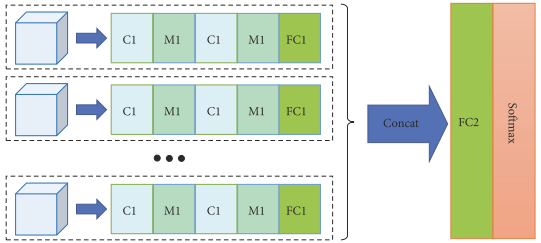
\includegraphics[width=0.7\linewidth]{images/Yang2019_Fig2}
	\caption{MCF-3DCNN architecture as detailed by \textbf{©Yang et al. \cite{Yang2019}}}
	\label{fig:Yang2019_Figure2_MCF-3DCNN}
\end{figure}


During the training process, they implemented a label-shuffling method
to overcome the problem of imbalanced data. Furthermore, to avoid the
effect of overfitting, they trained their network with augmented data
(original images were transposed, rotated, and flipped), a learning rate
reduction and the addition of dropout (rate = 0.5).
Using their architecture they were able to correctly classify the \ac{hcc}s
into the 3 differentiation groups with a mean accuracy of \textbf{74\%}.\\
Their study however suffers from a lot of limitations such as the
reduced size of the cohort, the imbalanced data and the fact that the
analysis was only performed in a manually drawn \ac{voi}.\\
We have decided to tackle the same issue, but we implemented a fully
automatic pipeline where both the segmentation and the grade prediction
steps were performed by \ac{dl} networks.

\section{Material}


To build an automatic histological grade prediction pipeline, we decided to extract relevant imaging features from our multiphase liver tumor semantic segmentation network. These features will then be processed by another neural network for the histological grade prediction. To build such an architecture we used 3 different datasets since none of the available datasets was consistent enough to be used alone (2 datasets were responsible for the training of the liver tumor segmentation through a 2-stages cascaded architecture and one for the training/testing of the histological grade prediction). The entire pipeline is described in the figure \ref{fig:DLR_pipeline_withDB}.
\begin{figure}[ht!]
	\centering
	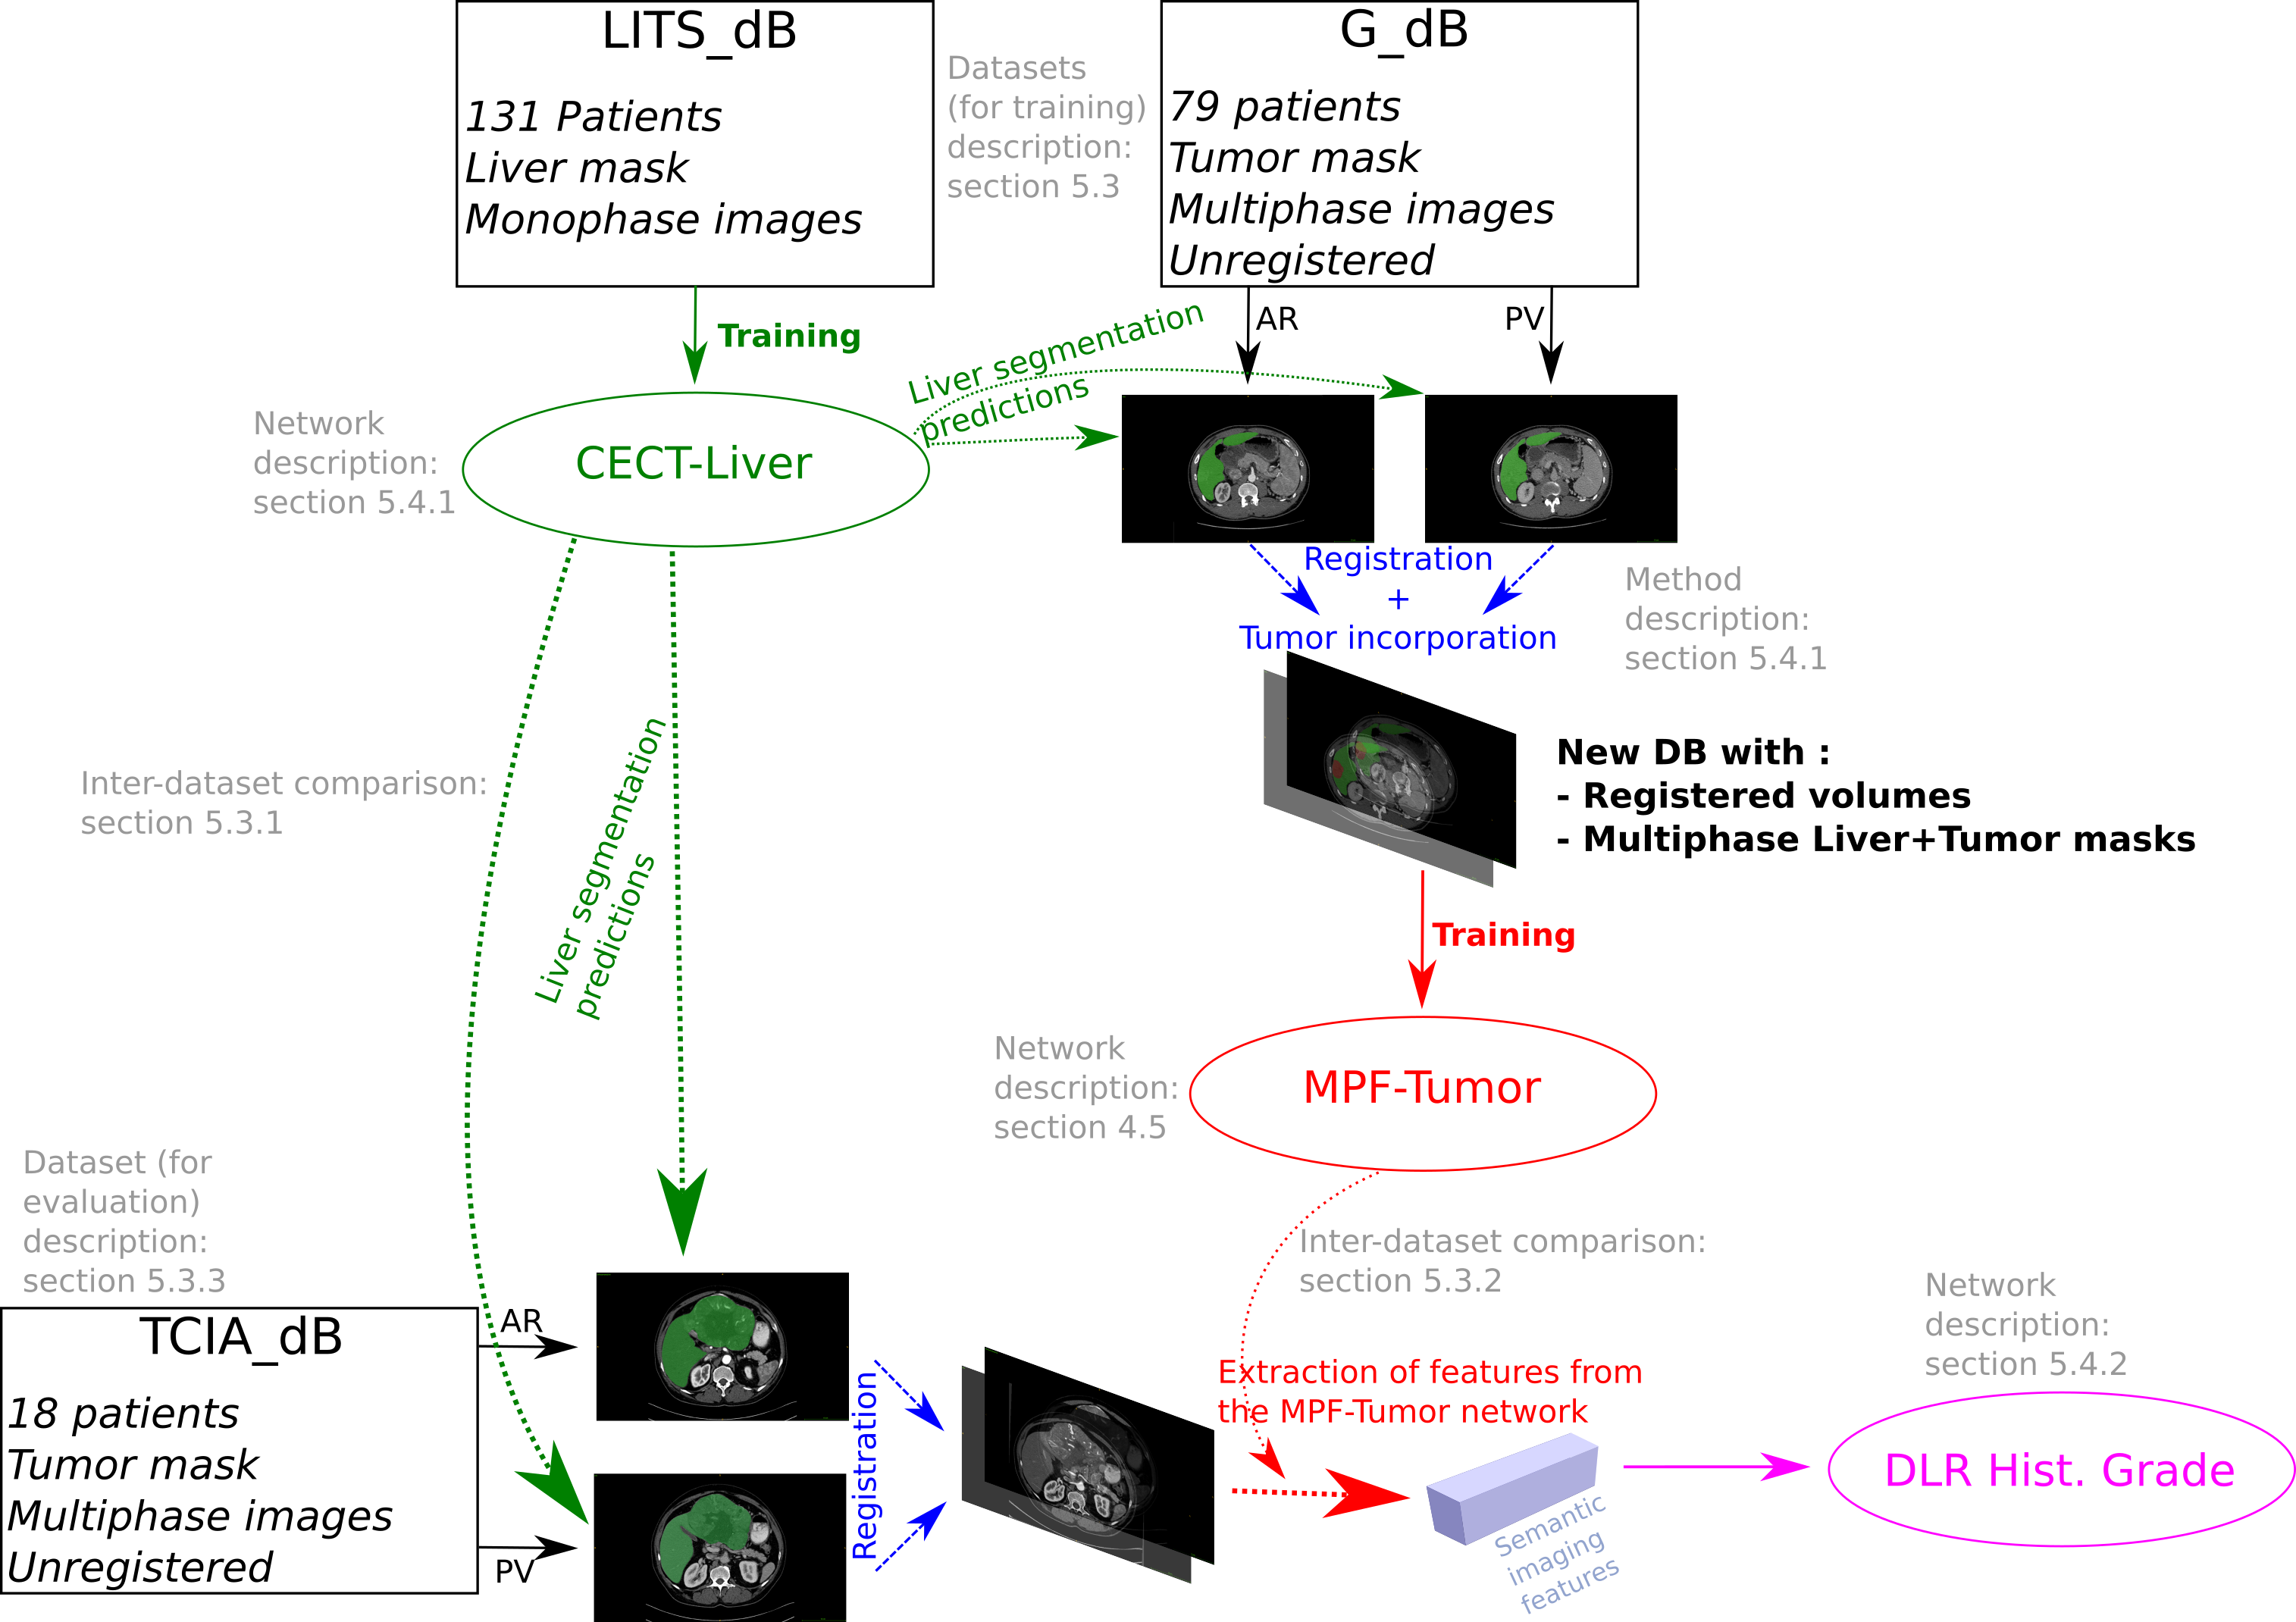
\includegraphics[width=0.9\linewidth]{../HistologicalGradePrediction/images/DLR_pipeline_withDB}
	\caption{Description of the entire workflow to build our DLR-based histological grade prediction. \textbf{\lmttfont{LITS-dB}} and \textbf{\lmttfont{G-dB}} are used to train respectively the liver (green arrows) and the liver tumor (red arrows) semantic segmentation network, whereas \textbf{\lmttfont{TCIA-dB}} is used to train the histological grade prediction using semantic imaging features extracted from the liver tumor segmentation network (pink arrow).}
	\label{fig:DLR_pipeline_withDB}
\end{figure}
%The only available dataset with histological grade expert ground truth is the \textbf{\lmttfont{TCIA-dB}} one, therefore, we first reimplemented a cascaded liver tumor semantic segmentation architecture before extracting imaging features to evaluate the histological grade prediction in a CV-manner on the \textbf{\lmttfont{TCIA-dB}} dataset. \\
We first trained a modified version of the automatic liver segmentation network (presented in the section \ref{subsect_auto_liver_tumor_seg}) using the 131 volumes of the \textbf{\lmttfont{LITS-dB}} dataset in order to segment the liver on both \ac{ar} and \ac{pv} phases independently. We then trained our \pplfont{MPF-Tumor} segmentation network using the 79 multiphase volumes of the \textbf{\lmttfont{G-dB}}. We subsequently evaluated the obtained tumor segmentation on the registered volumes of the \textbf{\lmttfont{TCIA-dB}} dataset. After the extraction of relevant imaging features, we performed a cross-validation training on the 18 multiphase volumes of the \textbf{\lmttfont{TCIA-dB}} to predict the histological grade. \\
Thereafter, we give more details about the inter-database differences, especially those between \textbf{\lmttfont{LITS-dB}} and \textbf{\lmttfont{TCIA-dB}} used respectively as training and testing datasets for the liver segmentation network, and those between \textbf{\lmttfont{G-dB}} and \textbf{\lmttfont{TCIA-dB}} used respectively as training and testing datasets for the liver tumor segmentation network.

\subsection{Liver segmentation inter-dataset comparison (\textbf{\lmttfont{LITS-dB}} vs \textbf{\lmttfont{TCIA-dB}})} \label{liver_interdb_comparison}

Our objective is to automatically segment the liver on both the \ac{ar} and the \ac{pv} phased volumes of the \textbf{\lmttfont{TCIA-dB}}. In the available datasets (as presented in the table \textbf{\textcolor{red}{ref table datasets}}), only \textbf{\lmttfont{TheraHCC-dB}} and \textbf{\lmttfont{LITS-dB}} contained expert liver delineation. \textbf{\lmttfont{TheraHCC-dB}} contains annotations only on sparse slices across the liver, whereas \textbf{\lmttfont{LITS-dB}} contains full 3D pixel-wise liver annotation but it only contains single-phase images, without any information regarding the
acquisition phase (\ac{ar}, \ac{pv} and potentially DELAY volumes are mixed in the dataset).
Regarding its design and the high number of segmented cases it contained, we decided to train our liver segmentation network using the \textbf{\lmttfont{LITS-dB}} volumes and test it on the \textbf{\lmttfont{TCIA-dB}} patients.\\
We inspected both datasets to assess if a liver segmentation network trained using the \textbf{\lmttfont{LITS-dB}} volumes could perform the wanted task. Therefore, a medical expert was asked to determine the differences between the two datasets with a visual examination of the CT volumes (inspection of the types of tumors present in both datasets, as long as the different artifacts that can affect the training, such as the presence of benign hepatic lesions, of fat accumulation or metallic artifacts) and through a quantitative analysis of the HU intensities after placement of ROIs (especially to prove the presence of cirrhotic patients in both datasets and for the comparison between AR and PV labeled volumes in both datasets). \\
For the visual examination, the medical expert observed that both datasets contained liver volumes affected by large solitary tumors (HCC-like lesions), but some other smaller solitary tumors have also been found in both datasets, as depicted in the figure \ref{fig:interdb_tumorExamples}. It is worth noting that only the \textbf{\lmttfont{LITS-dB}} contained volumes with multiple lesions suspected to be metastases, as illustrated in the figure \ref{fig:litsDb_meta}. Both datasets presented livers with benign lesions, track of fat deposit, or other metallic artifacts, as illustrated in the figure \ref{fig:InterDb_artifacts}. Diseased livers were also present in both datasets, where severe signs of cirrhosis were noticed, as exposed in the figure \ref{fig:InterDb_diseasedLivers}.

\begin{figure}[!ht]
	\centering
	\begin{minipage}{0.45\linewidth}
		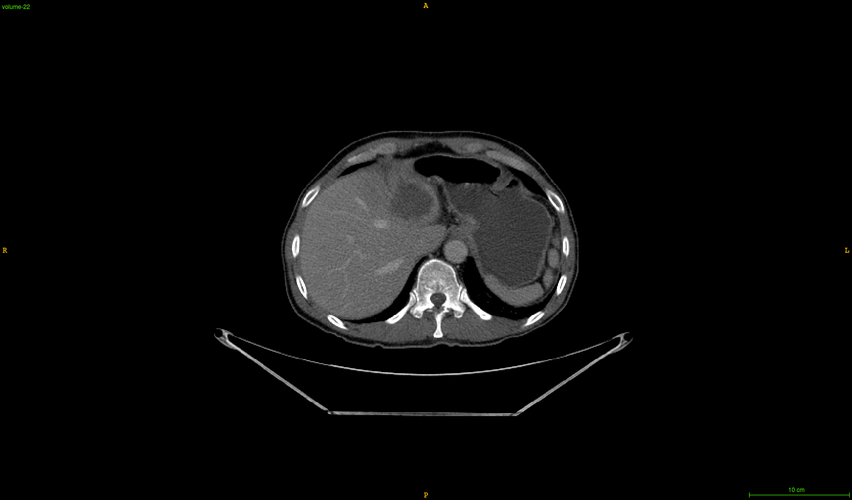
\includegraphics[width=\linewidth]{../Contributions/images/ResizeLITS_examplePatientSmallTumor_2}
	\end{minipage} \hspace{-0.1cm}
	\begin{minipage}{0.45\linewidth}
		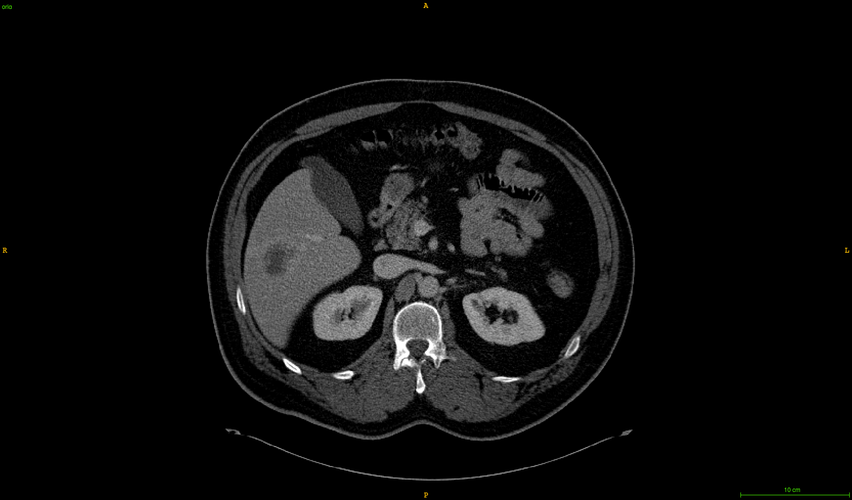
\includegraphics[width=\linewidth]{../Contributions/images/ResizeTCIA_examplePatientSmallTumor}
	\end{minipage} \\
	\begin{minipage}{0.45\linewidth}
		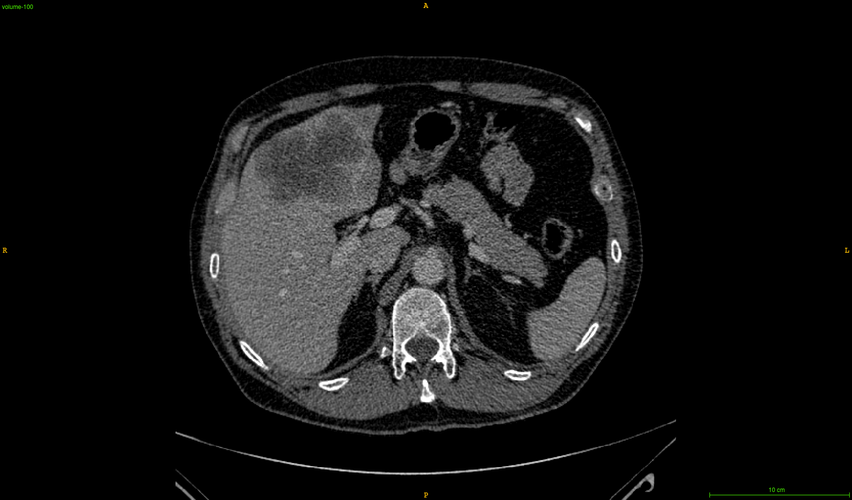
\includegraphics[width=\linewidth]{../Contributions/images/ResizeLITS_examplePatientLargeTumor}
	\end{minipage} \hspace{-0.1cm}
	\begin{minipage}{0.45\linewidth}
		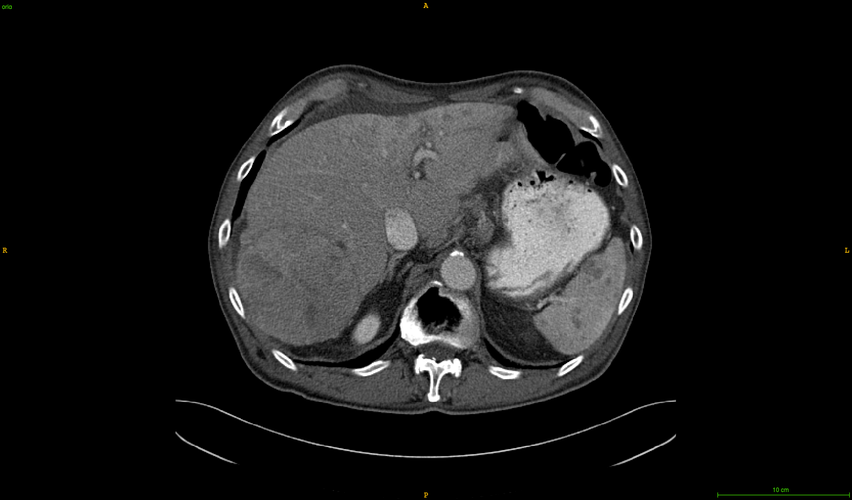
\includegraphics[width=\linewidth]{../Contributions/images/ResizeTCIA_examplePatientLargeTumor}
	\end{minipage}
	\caption{Example of small and large tumors from both the training and the testing datasets. Left: \textbf{\lmttfont{LITS-dB}} images, right: \textbf{\lmttfont{TCIA-dB}} images, top: small tumors, bottom: large tumors.}
	\label{fig:interdb_tumorExamples}
\end{figure}
\begin{figure}[!ht]
	\centering
	\begin{minipage}{0.45\linewidth}
		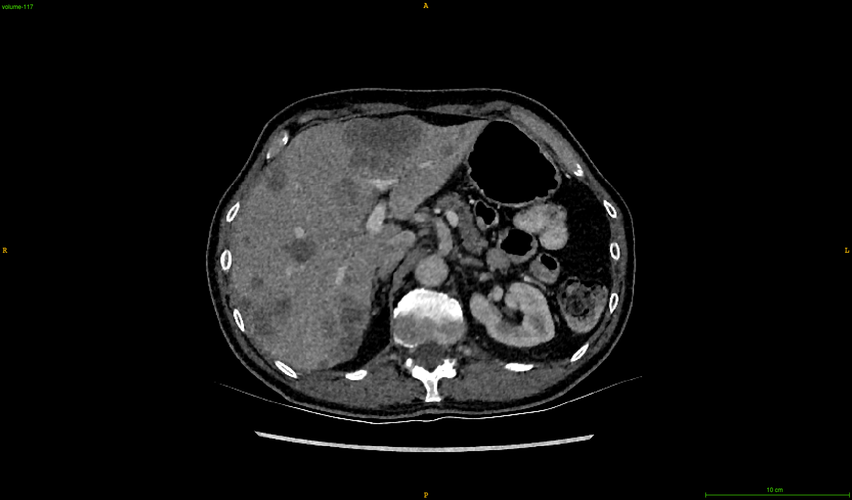
\includegraphics[width=\linewidth]{../Contributions/images/ResizeLITS_examplePatientMeta}
	\end{minipage} \hspace{-0.1cm}
	\begin{minipage}{0.45\linewidth}
		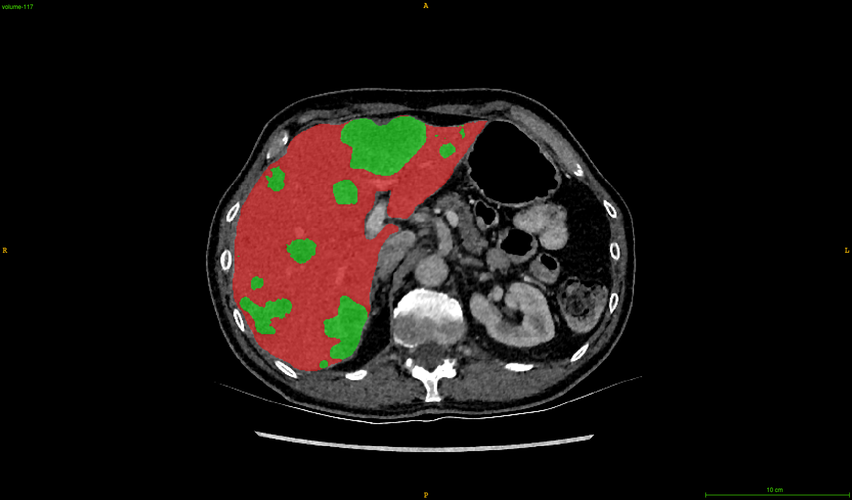
\includegraphics[width=\linewidth]{../Contributions/images/ResizeLITS_examplePatientMeta_seg}
	\end{minipage}
	\caption{Example of patient from the \textbf{\lmttfont{LITS-dB}} with a high number of tumors susceptible of being metastases. Right : raw image, left: expert segmentation where red represents liver parenchyma and green represents tumors.}
	\label{fig:litsDb_meta}
\end{figure}
\begin{figure}[!ht]
	\centering
	\begin{minipage}{0.45\linewidth}
		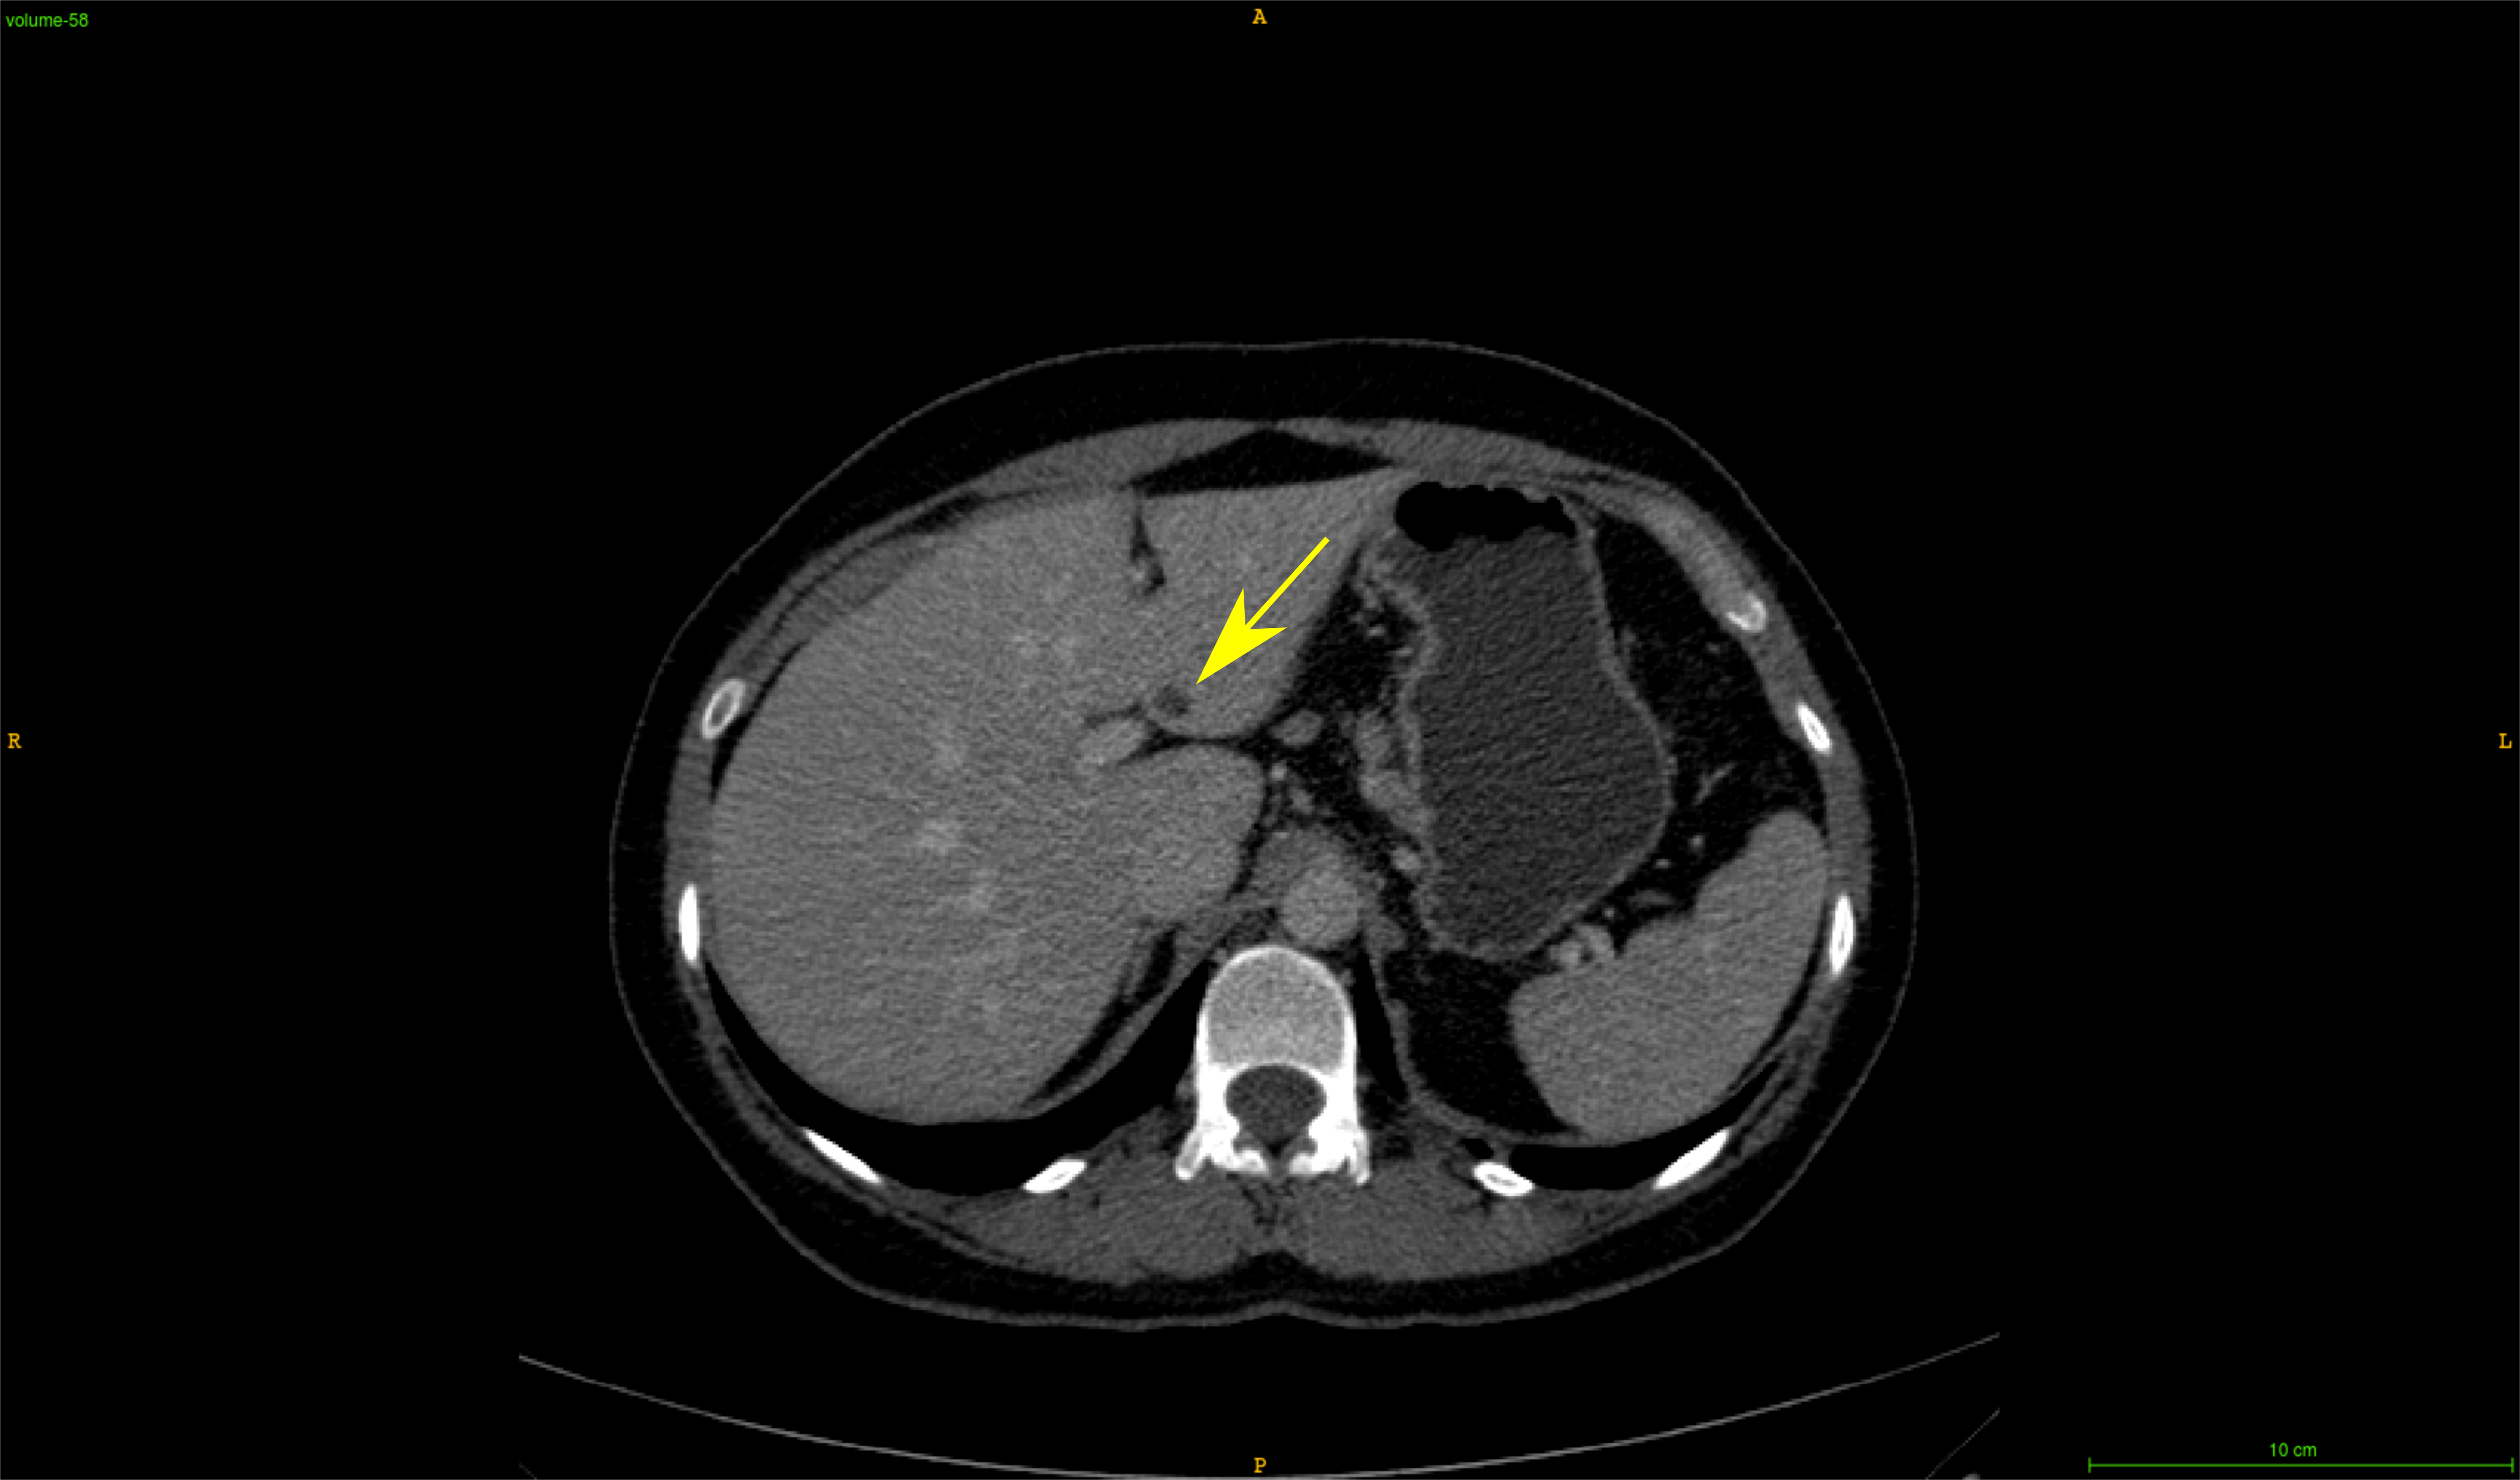
\includegraphics[width=\linewidth]{../Contributions/images/Artifacts/ResizeLITS_cyst}
	\end{minipage} \hspace{-0.1cm}
	\begin{minipage}{0.45\linewidth}
		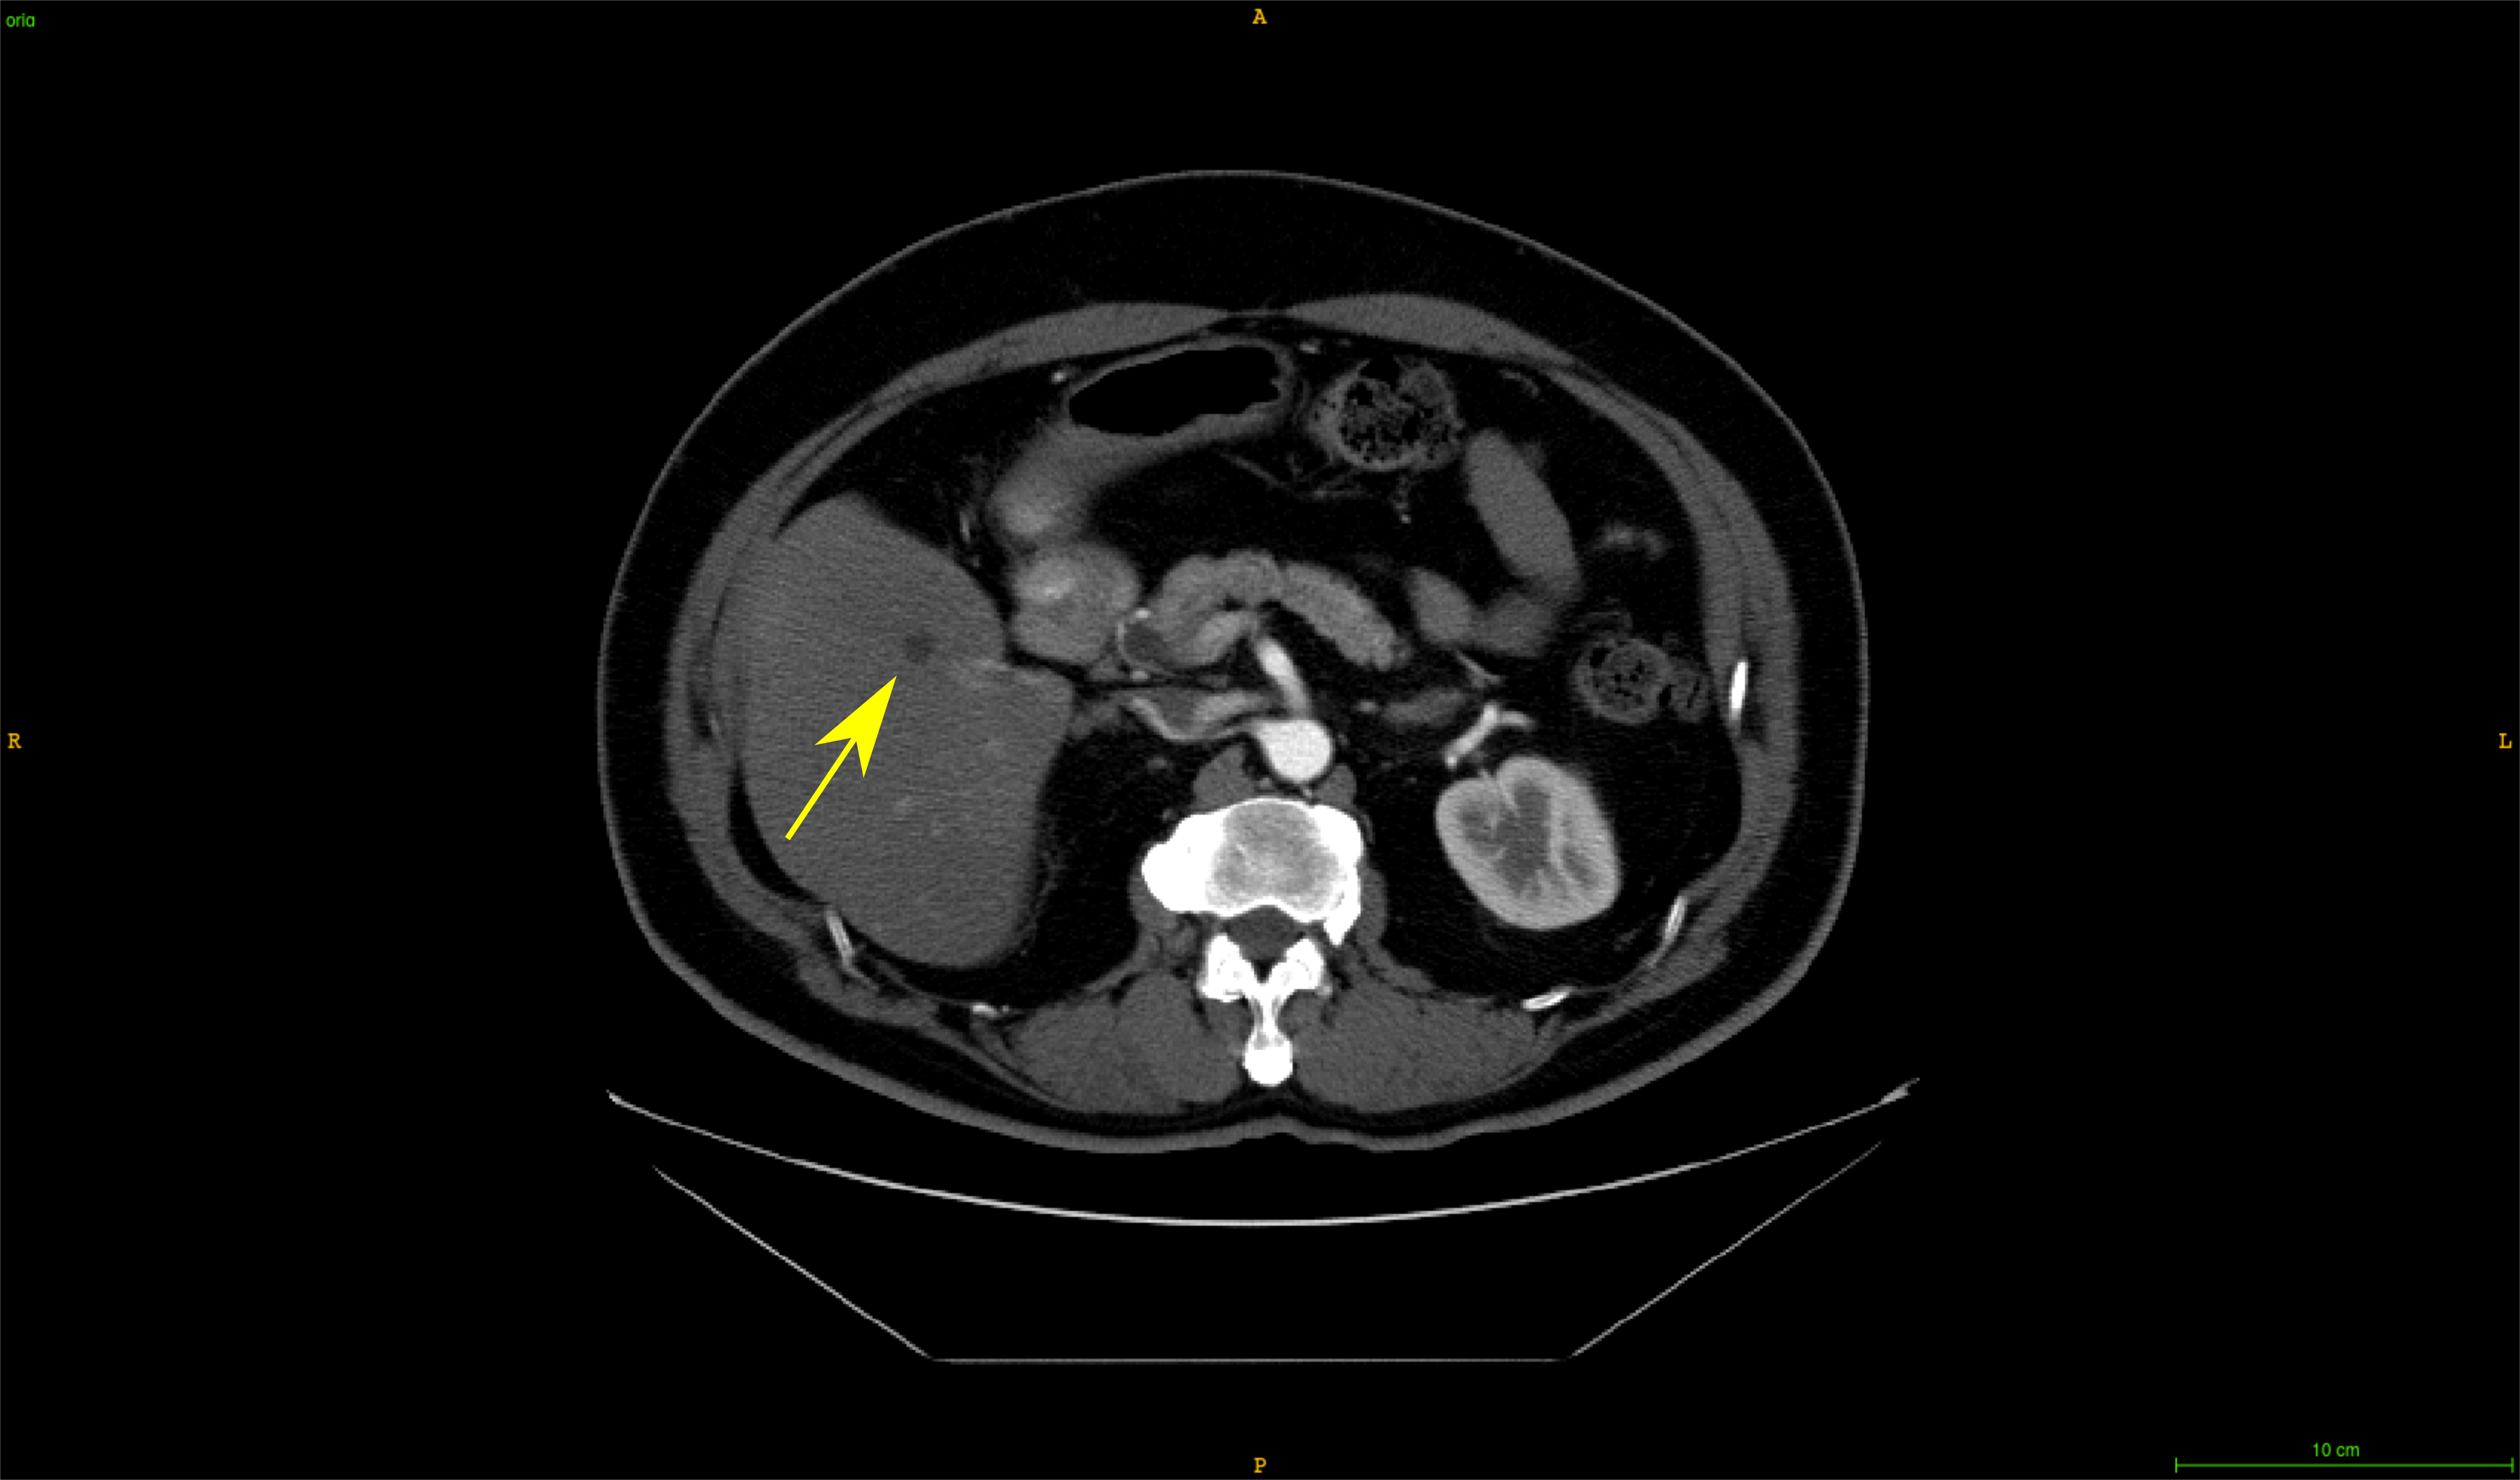
\includegraphics[width=\linewidth]{../Contributions/images/Artifacts/ResizeTCIA_cyst}
	\end{minipage} \\
	\begin{minipage}{0.45\linewidth}
		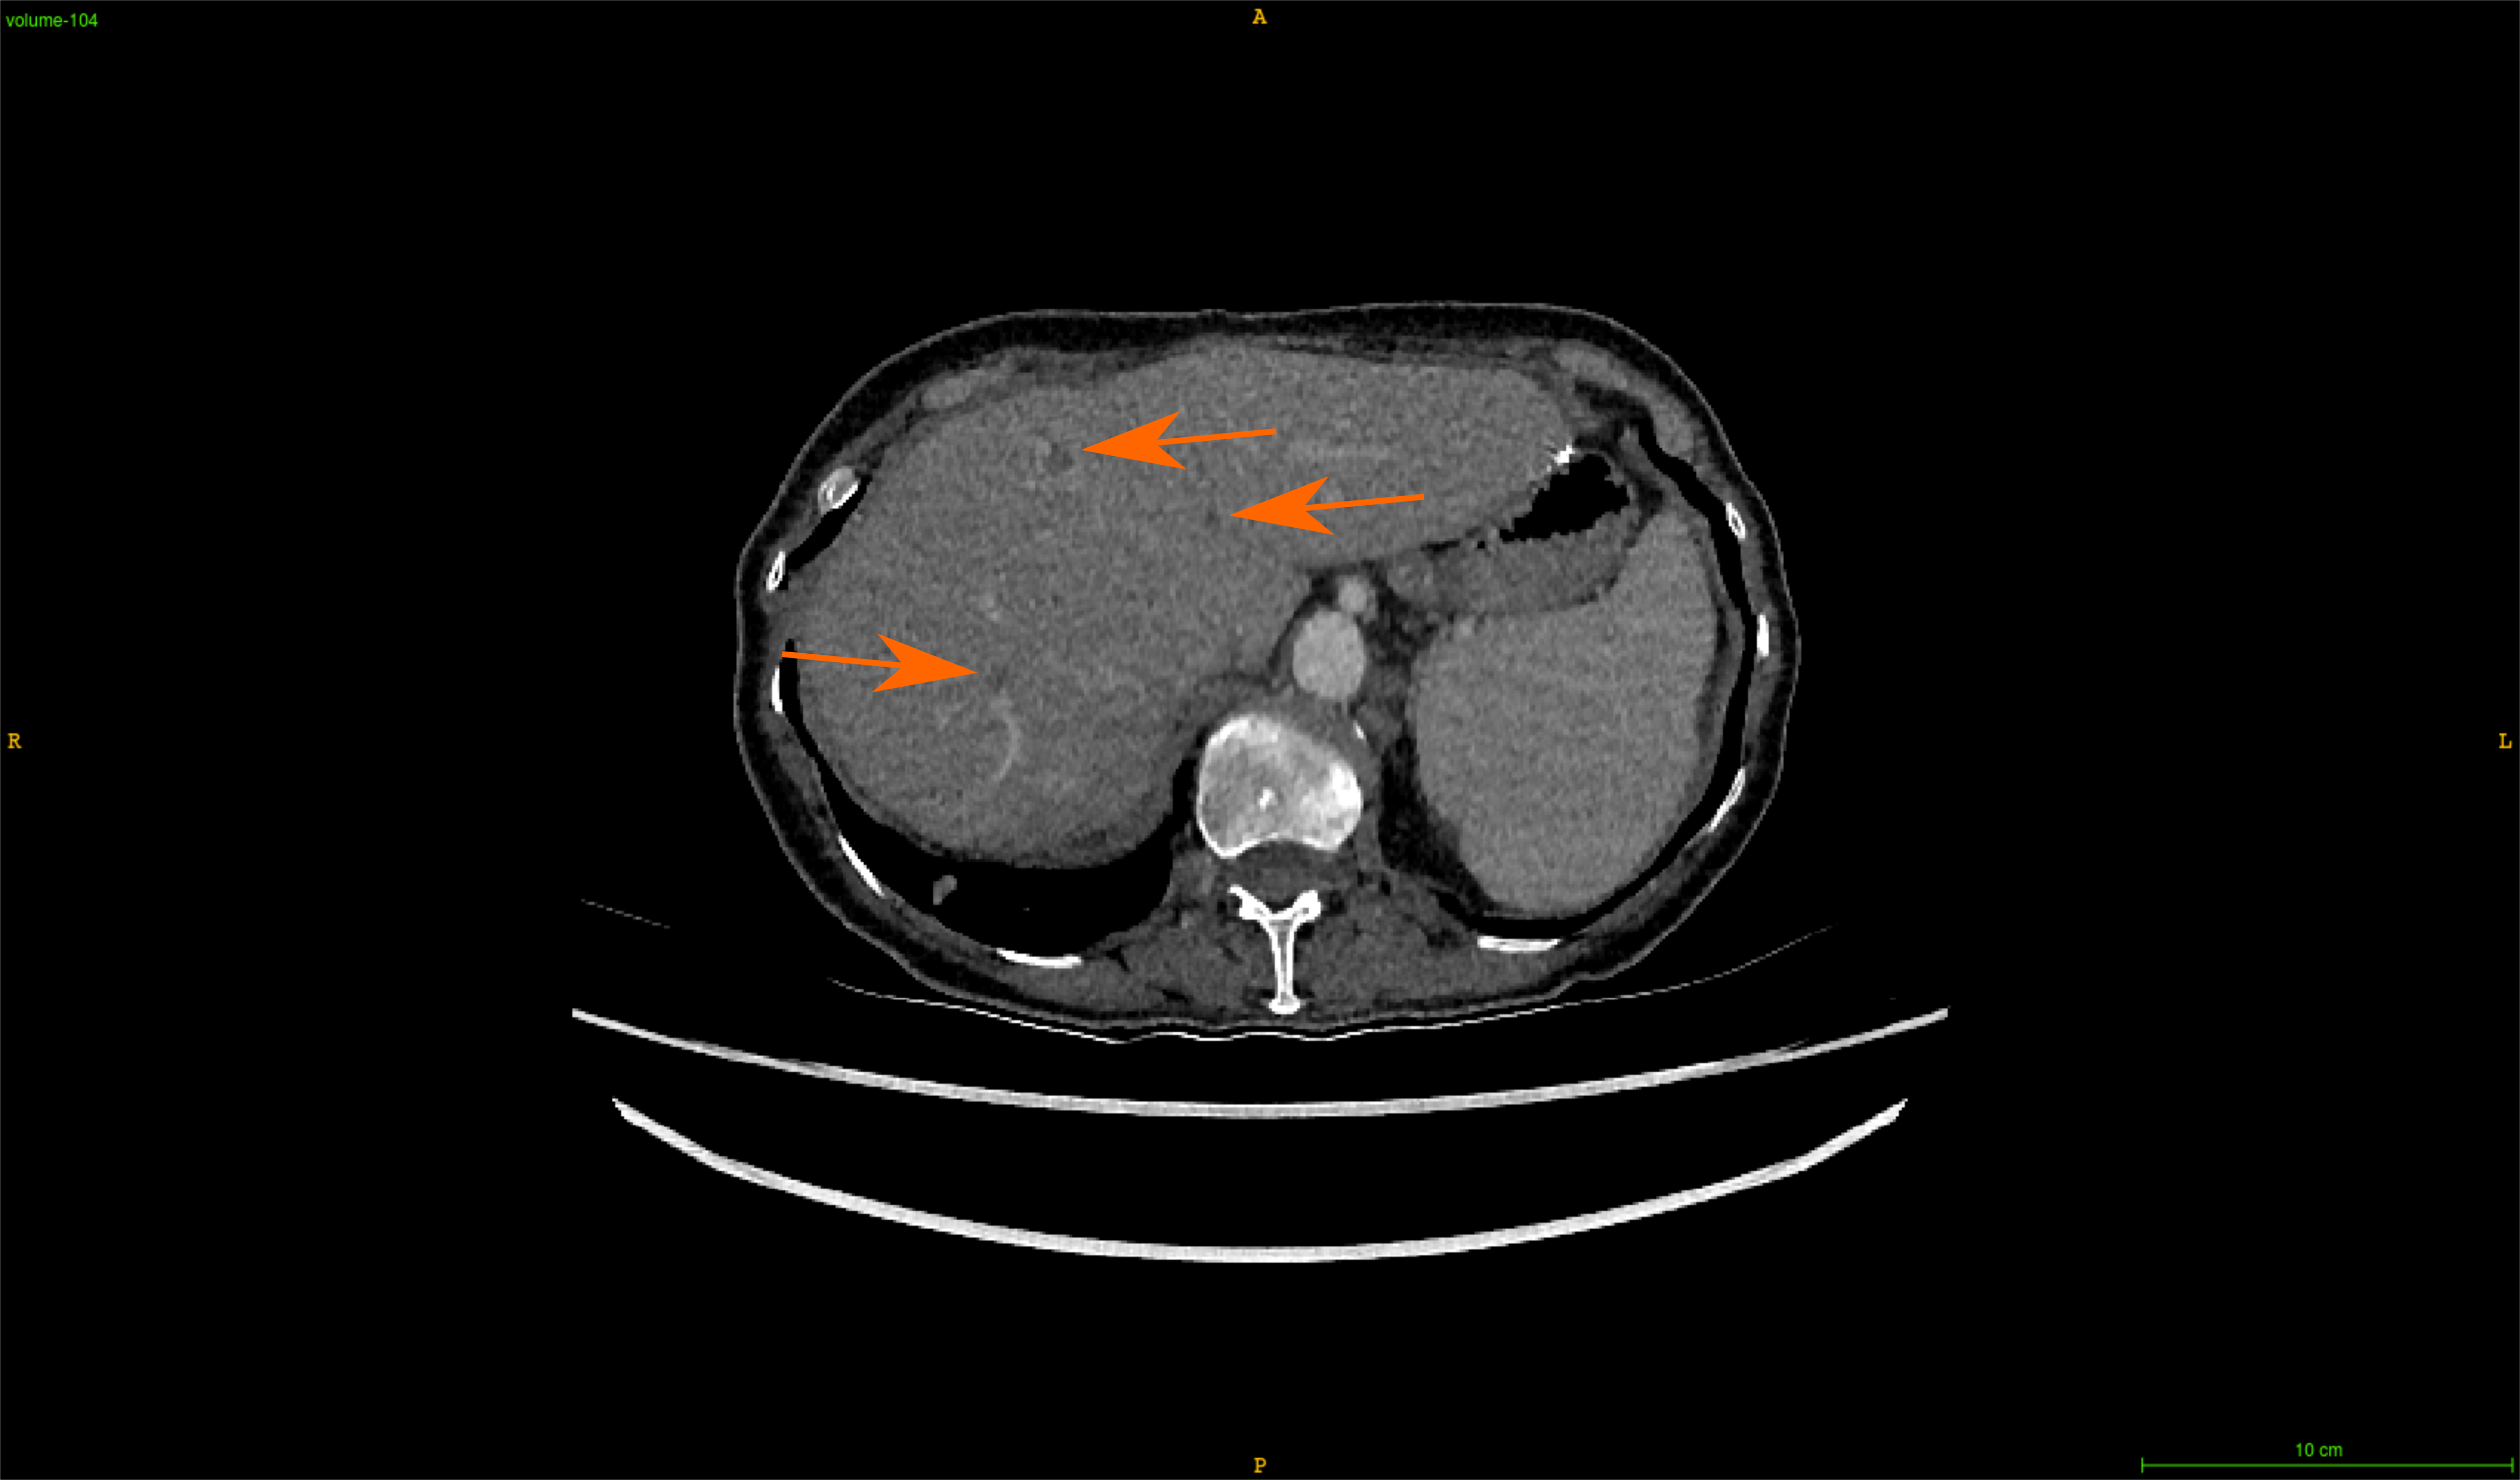
\includegraphics[width=\linewidth]{../Contributions/images/Artifacts/ResizeLITS_fat}
	\end{minipage} \hspace{-0.1cm}
	\begin{minipage}{0.45\linewidth}
		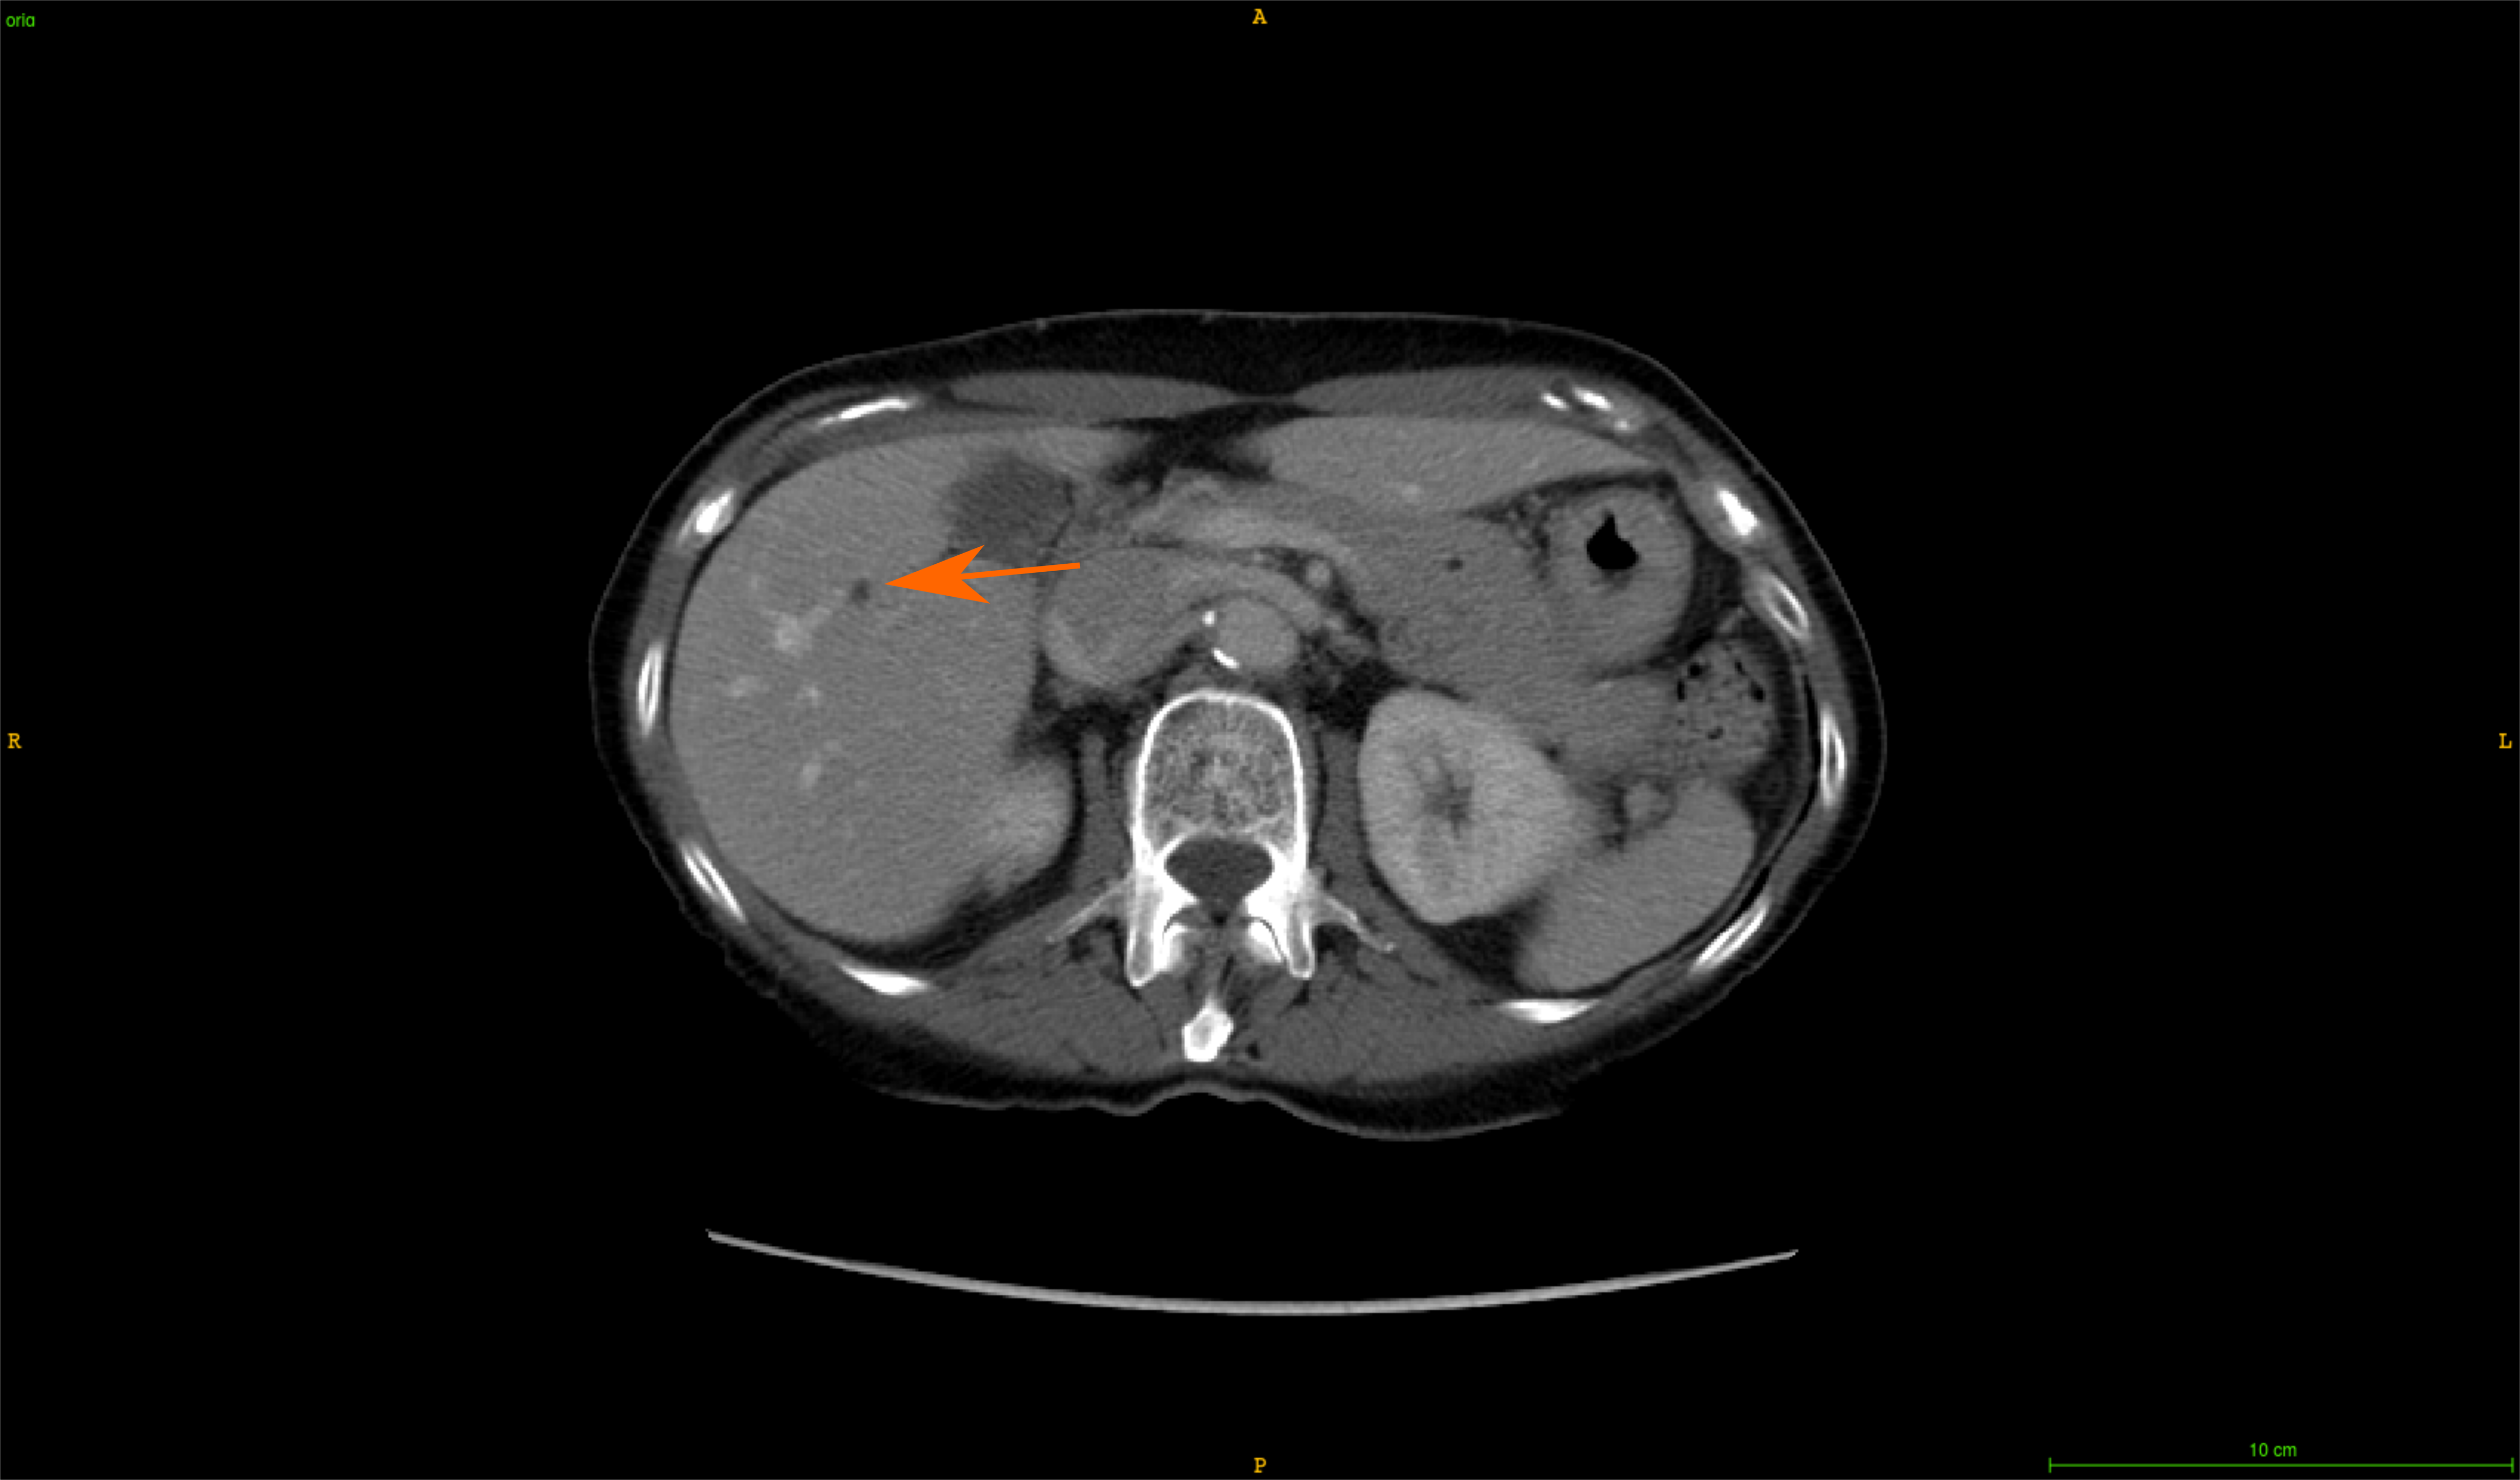
\includegraphics[width=\linewidth]{../Contributions/images/Artifacts/ResizeTCIA_fat}
	\end{minipage} \\
	\begin{minipage}{0.45\linewidth}
		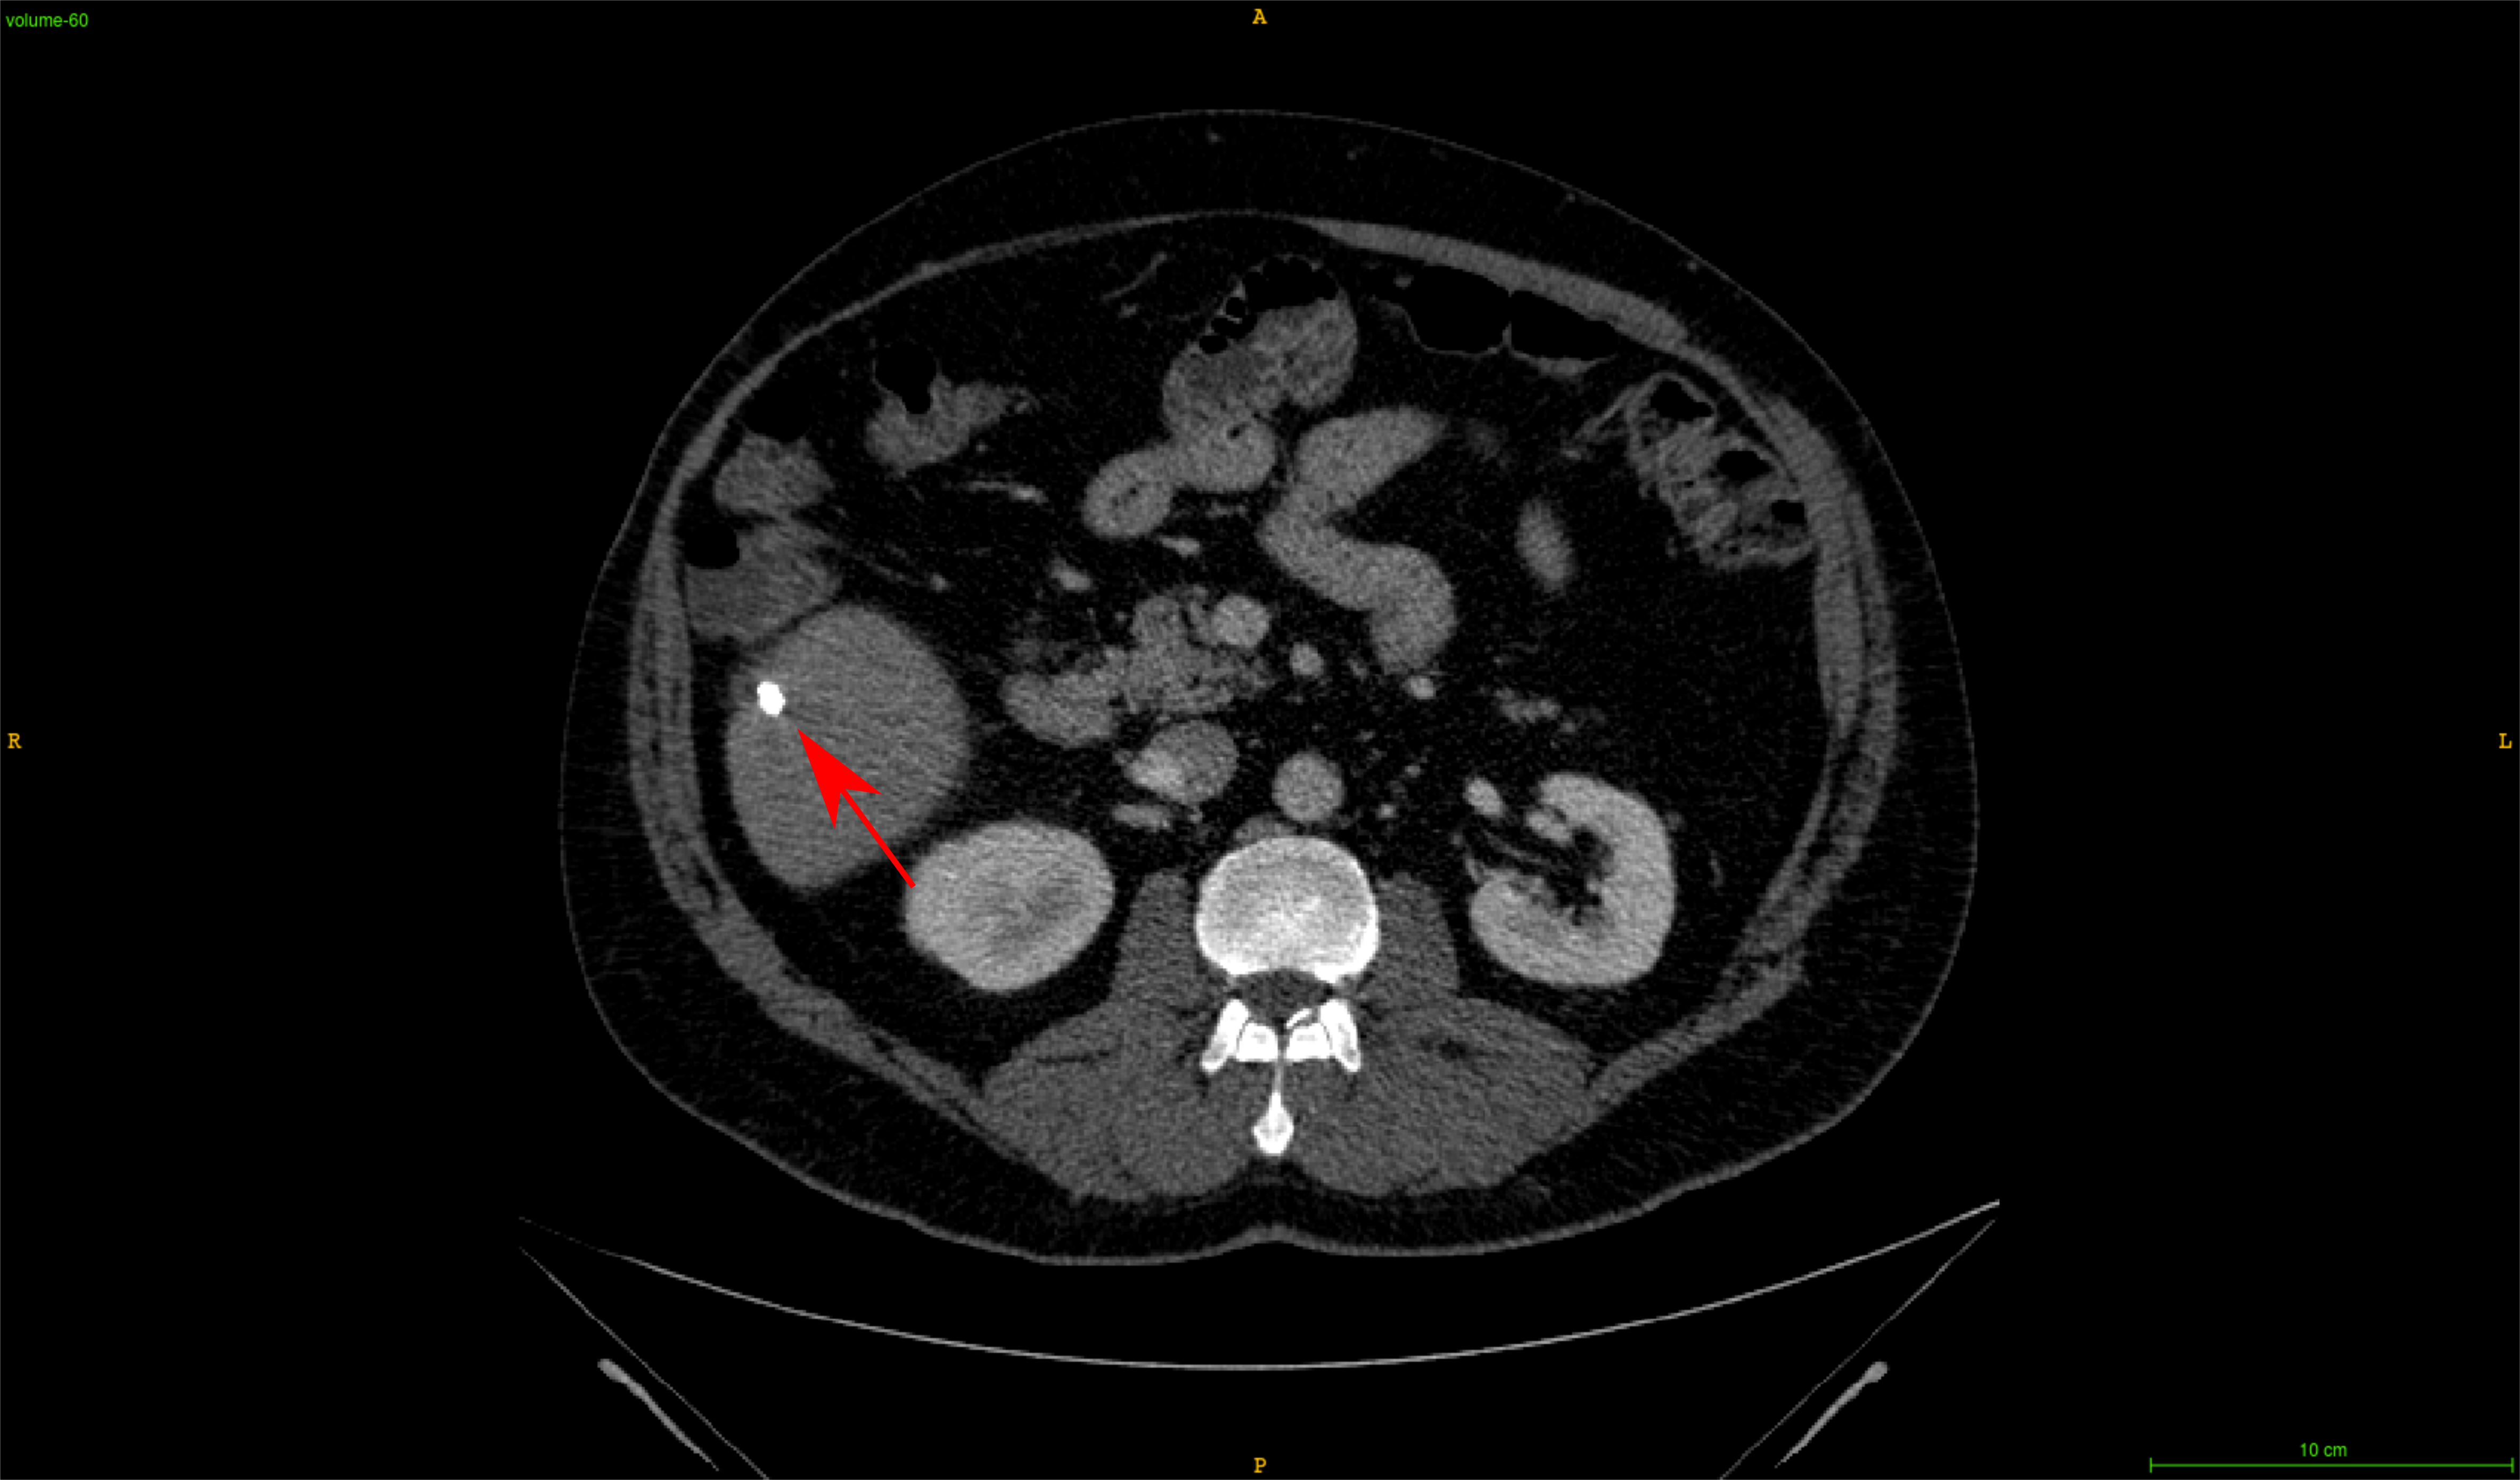
\includegraphics[width=\linewidth]{../Contributions/images/Artifacts/ResizeLITS_metallic_artifacts}
	\end{minipage} \hspace{-0.1cm}
	\begin{minipage}{0.45\linewidth}
		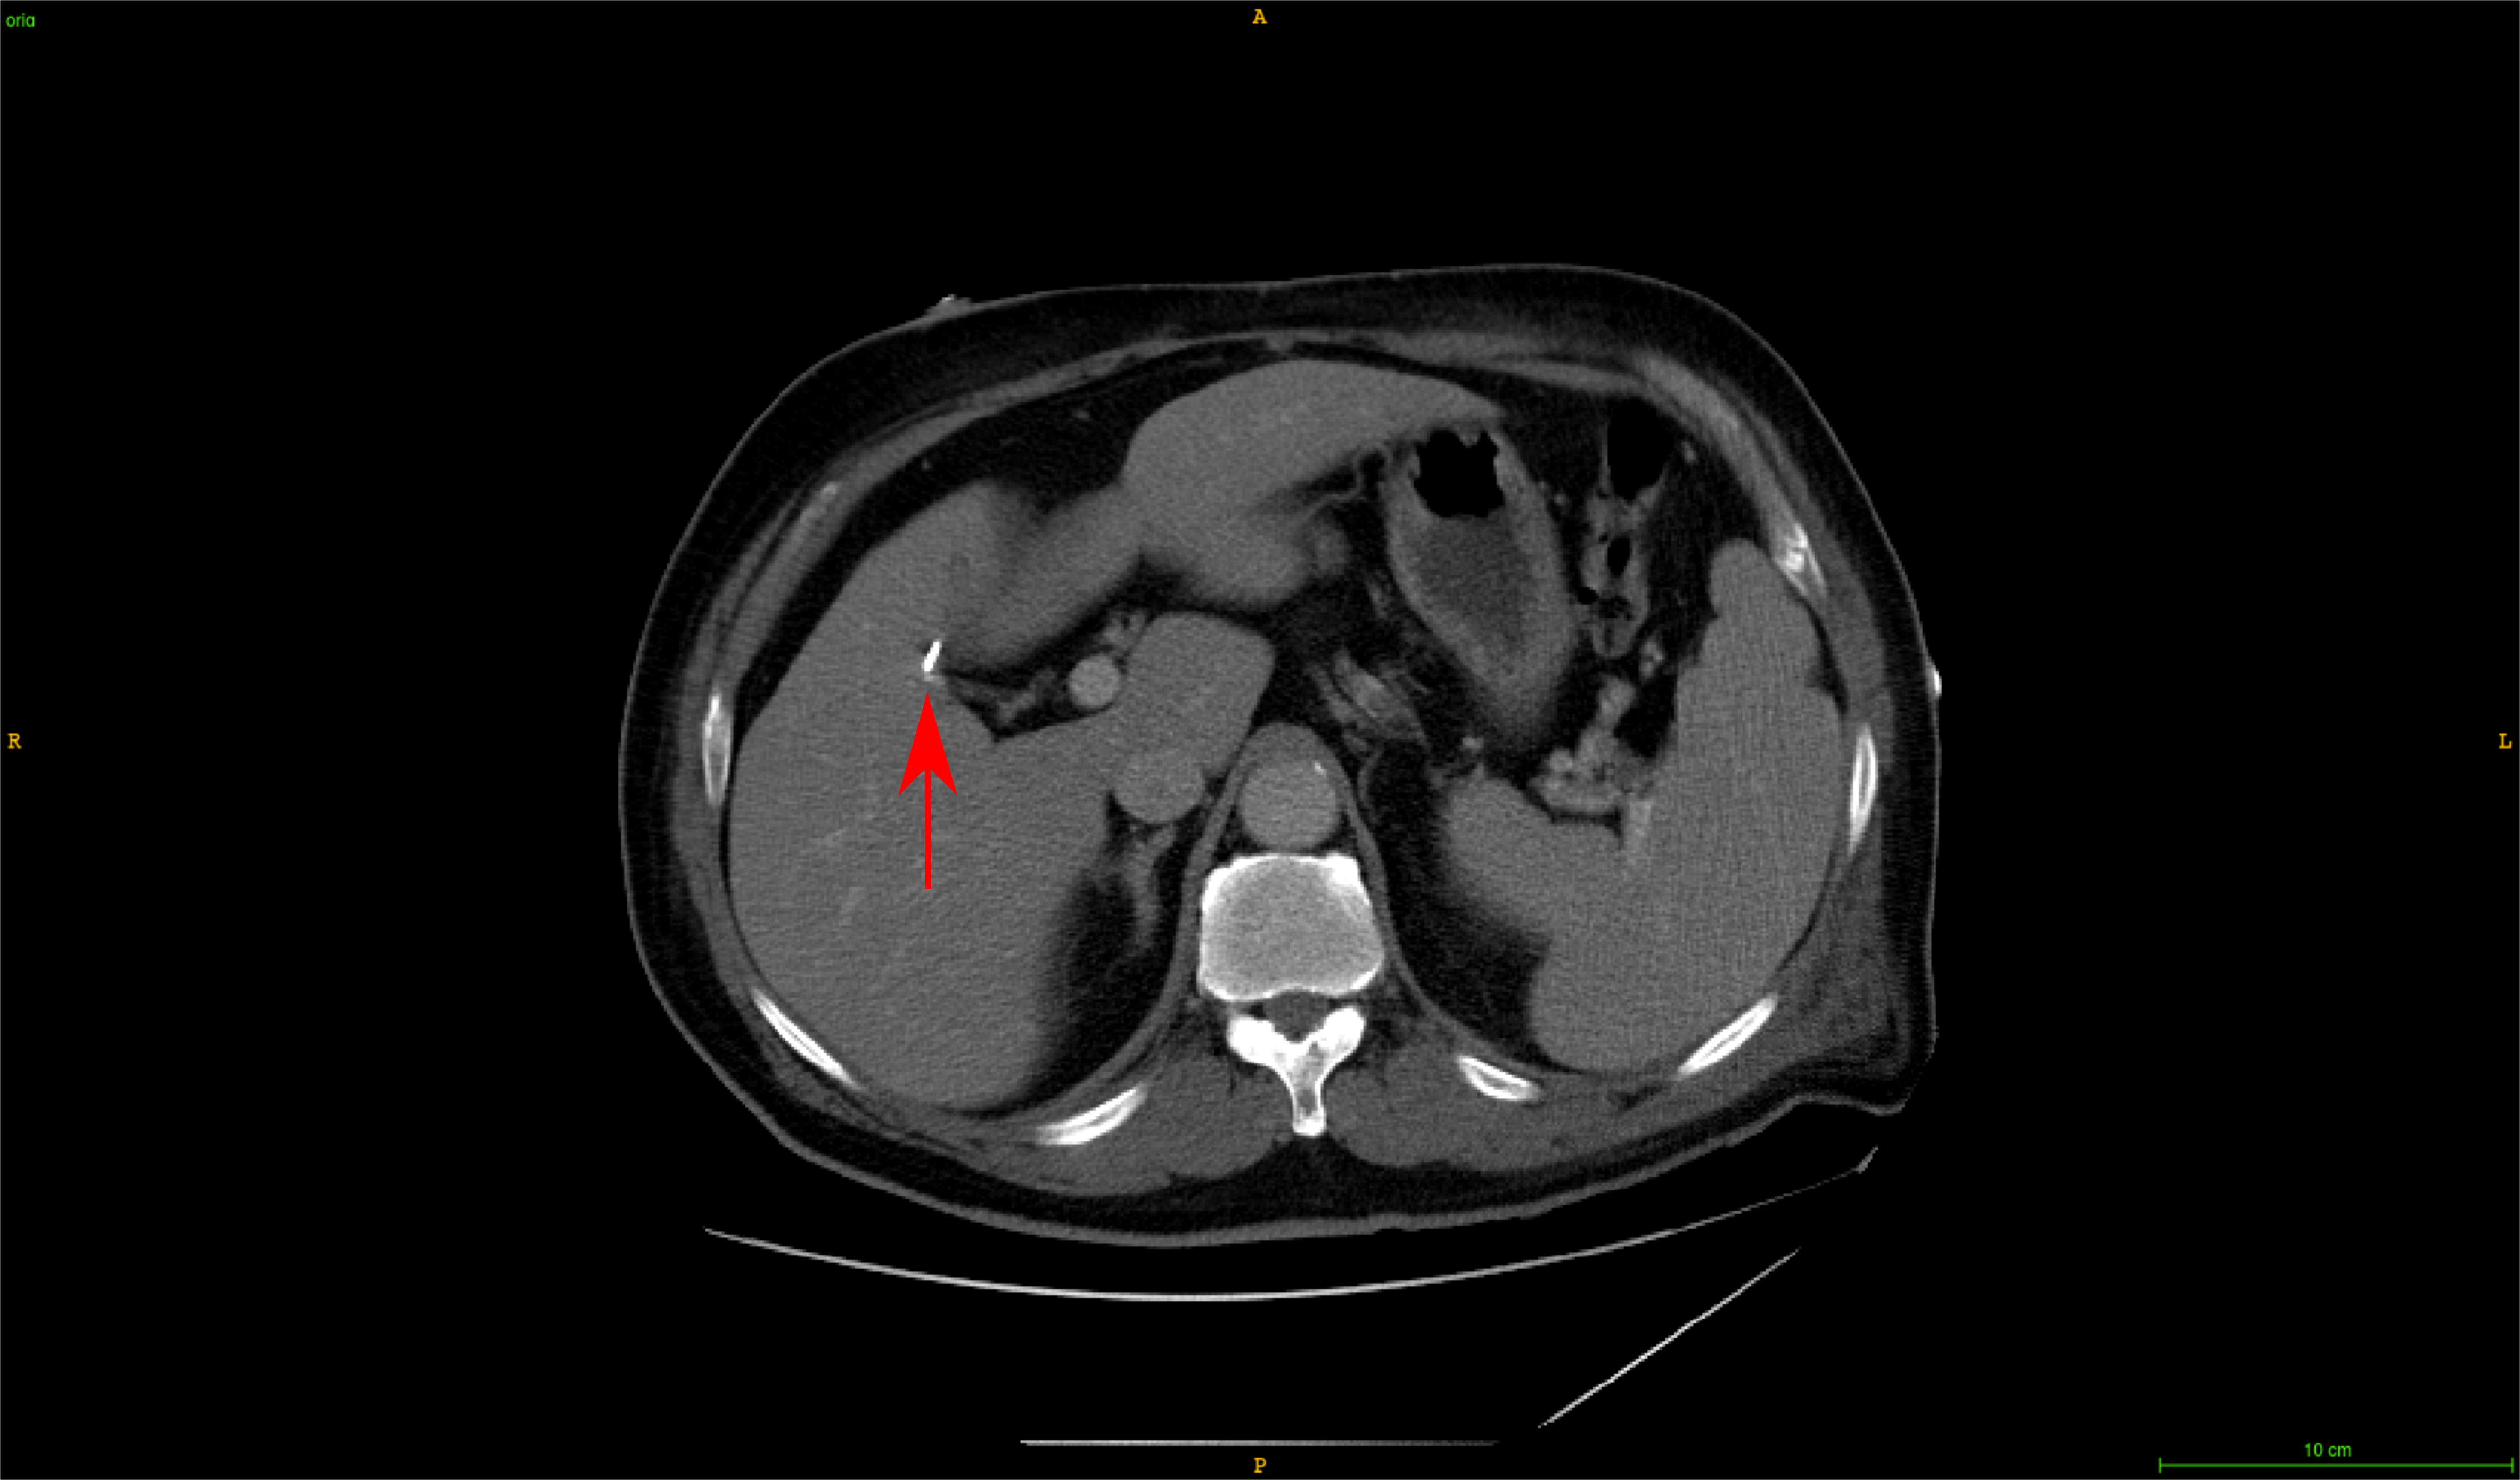
\includegraphics[width=\linewidth]{../Contributions/images/Artifacts/ResizeTCIA_metallic_artifacts}
	\end{minipage}
	\caption{Example of artifacts present in both training and test datasets. Left: \textbf{\lmttfont{LITS-dB}} images, right: \textbf{\lmttfont{TCIA-dB}} images. First row presents patients with benign hepatic lesions (yellow arrows), the second row presents liver with tracks of fat accumulation (orange arrows), whereas the last row gives examples of images with presence of metallic artifacts (red arrows).}
	\label{fig:InterDb_artifacts}
\end{figure}
\begin{figure}[!ht]
	\centering
	\begin{minipage}{0.45\linewidth}
		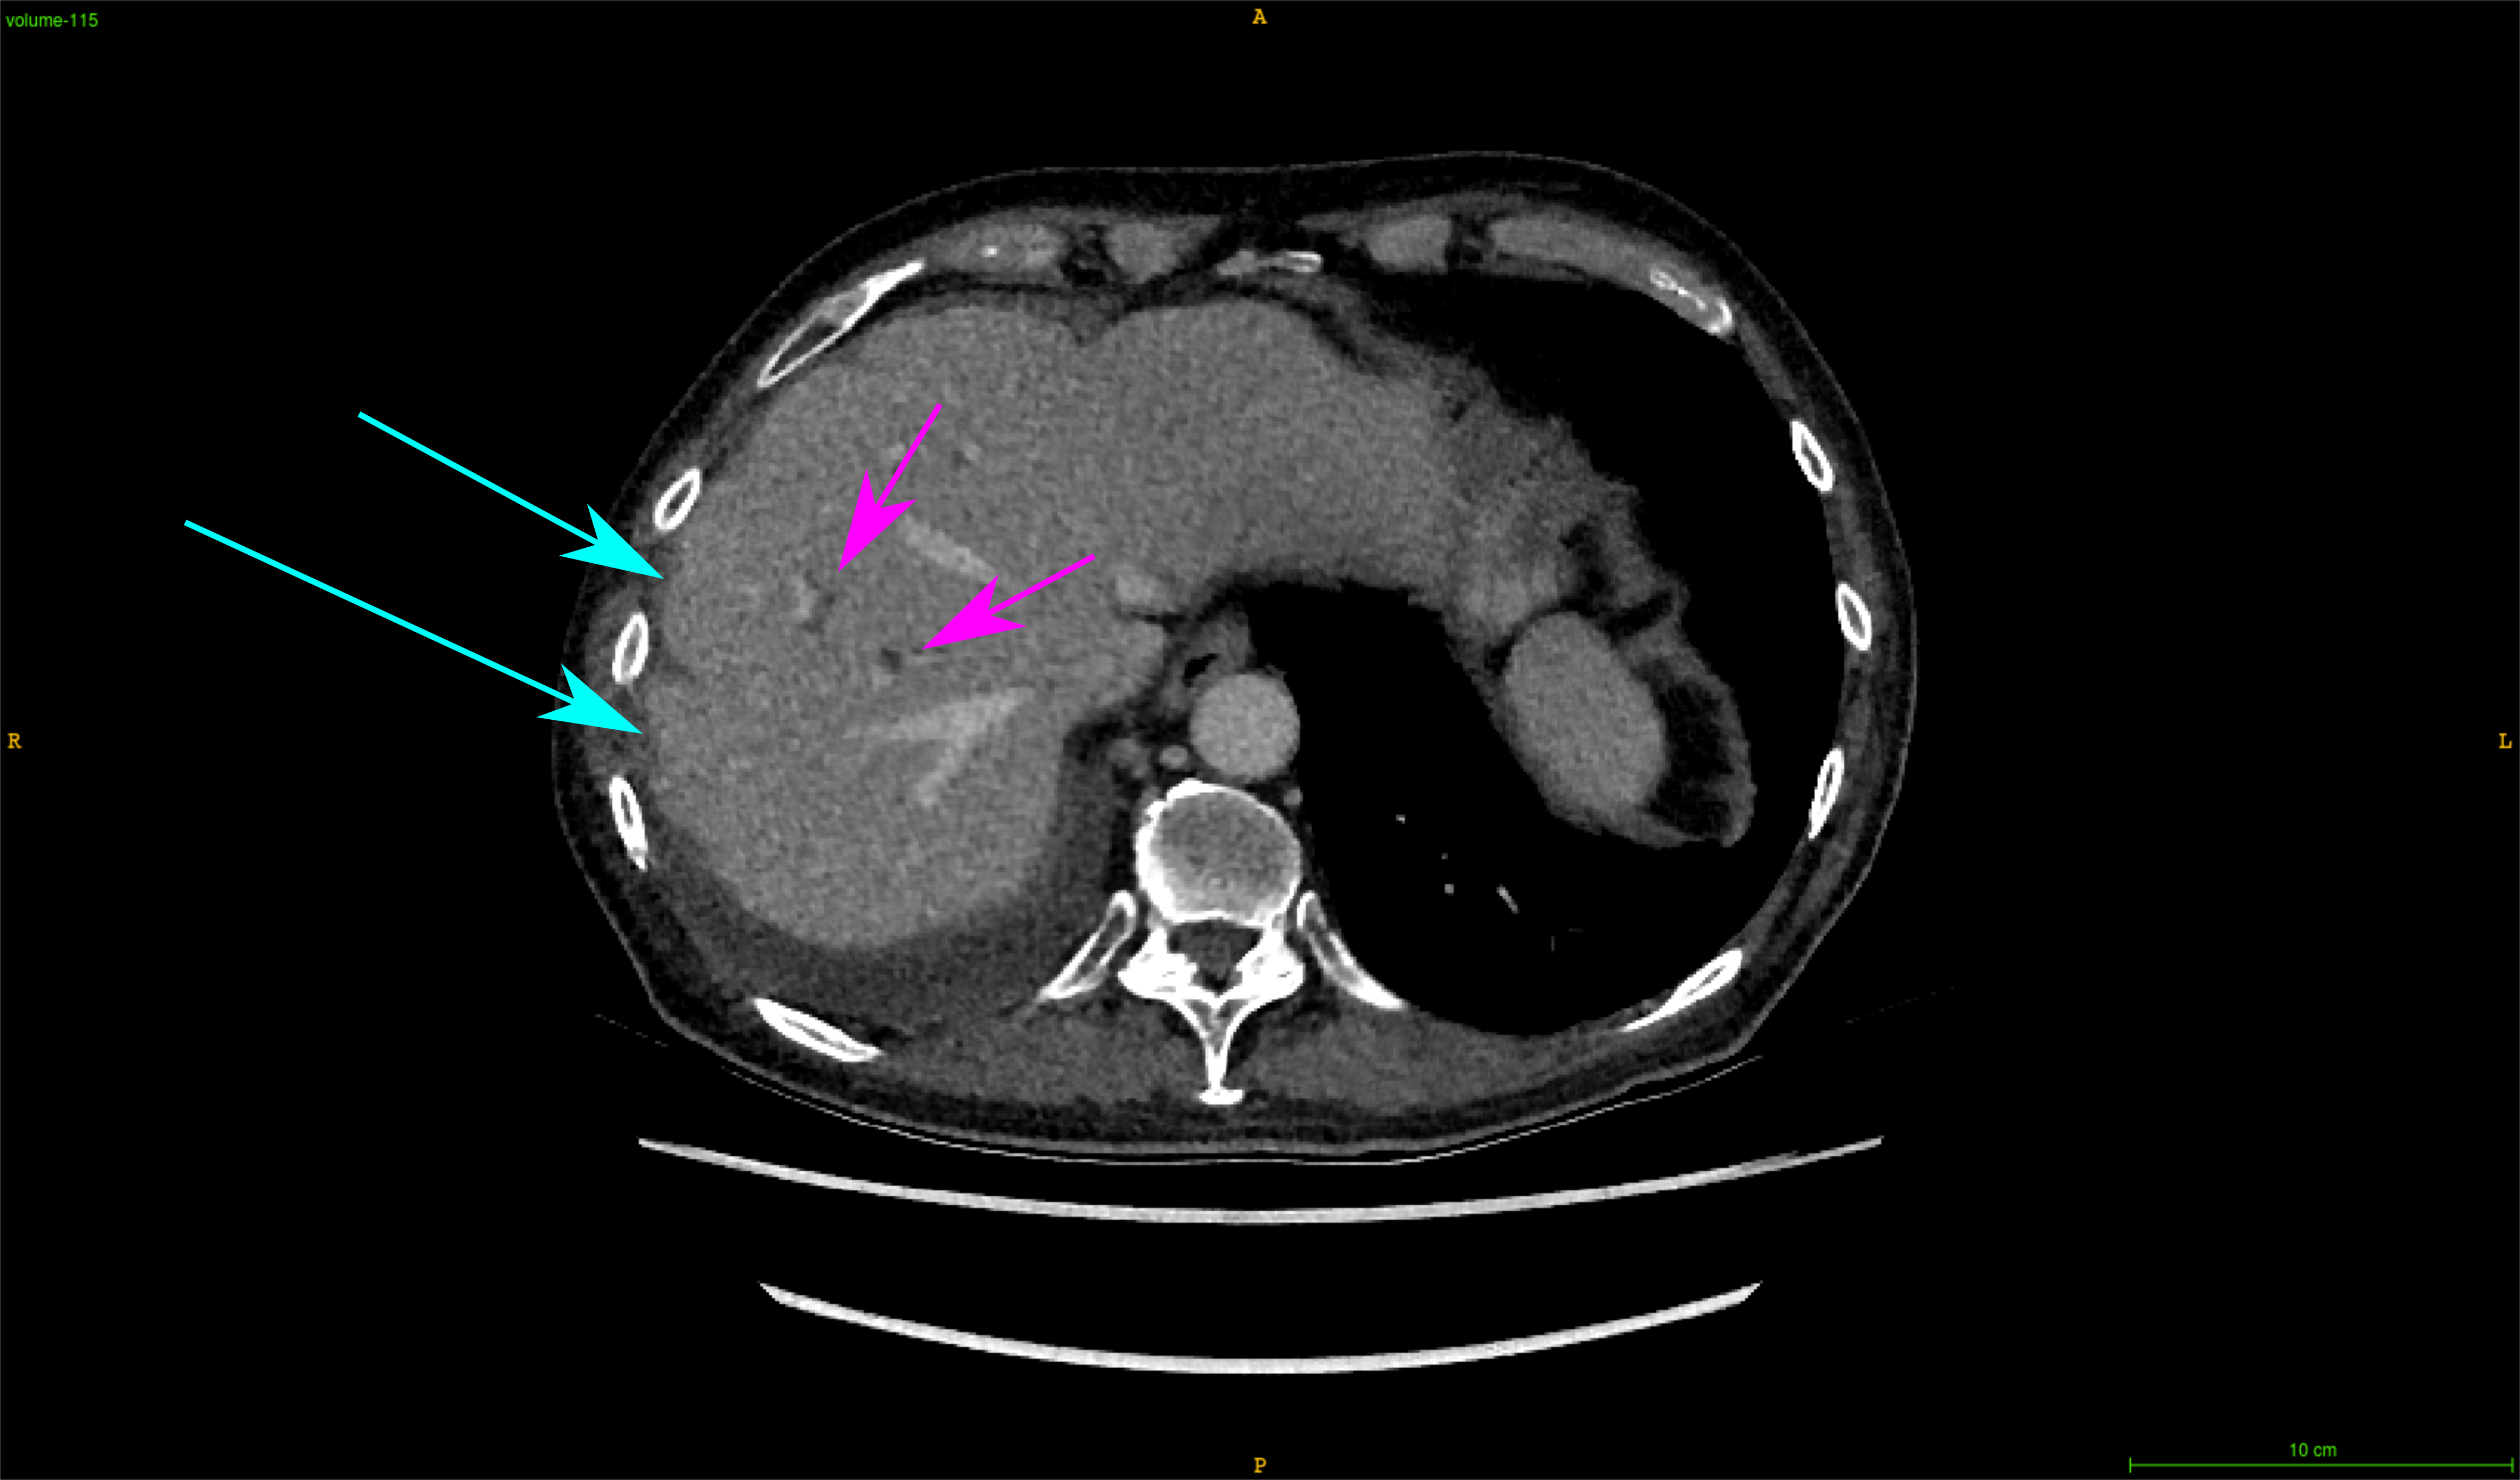
\includegraphics[width=\linewidth]{../Contributions/images/ResizeLITS_cirrhoticPatientArrows}
	\end{minipage} \hspace{-0.1cm}
	\begin{minipage}{0.45\linewidth}
		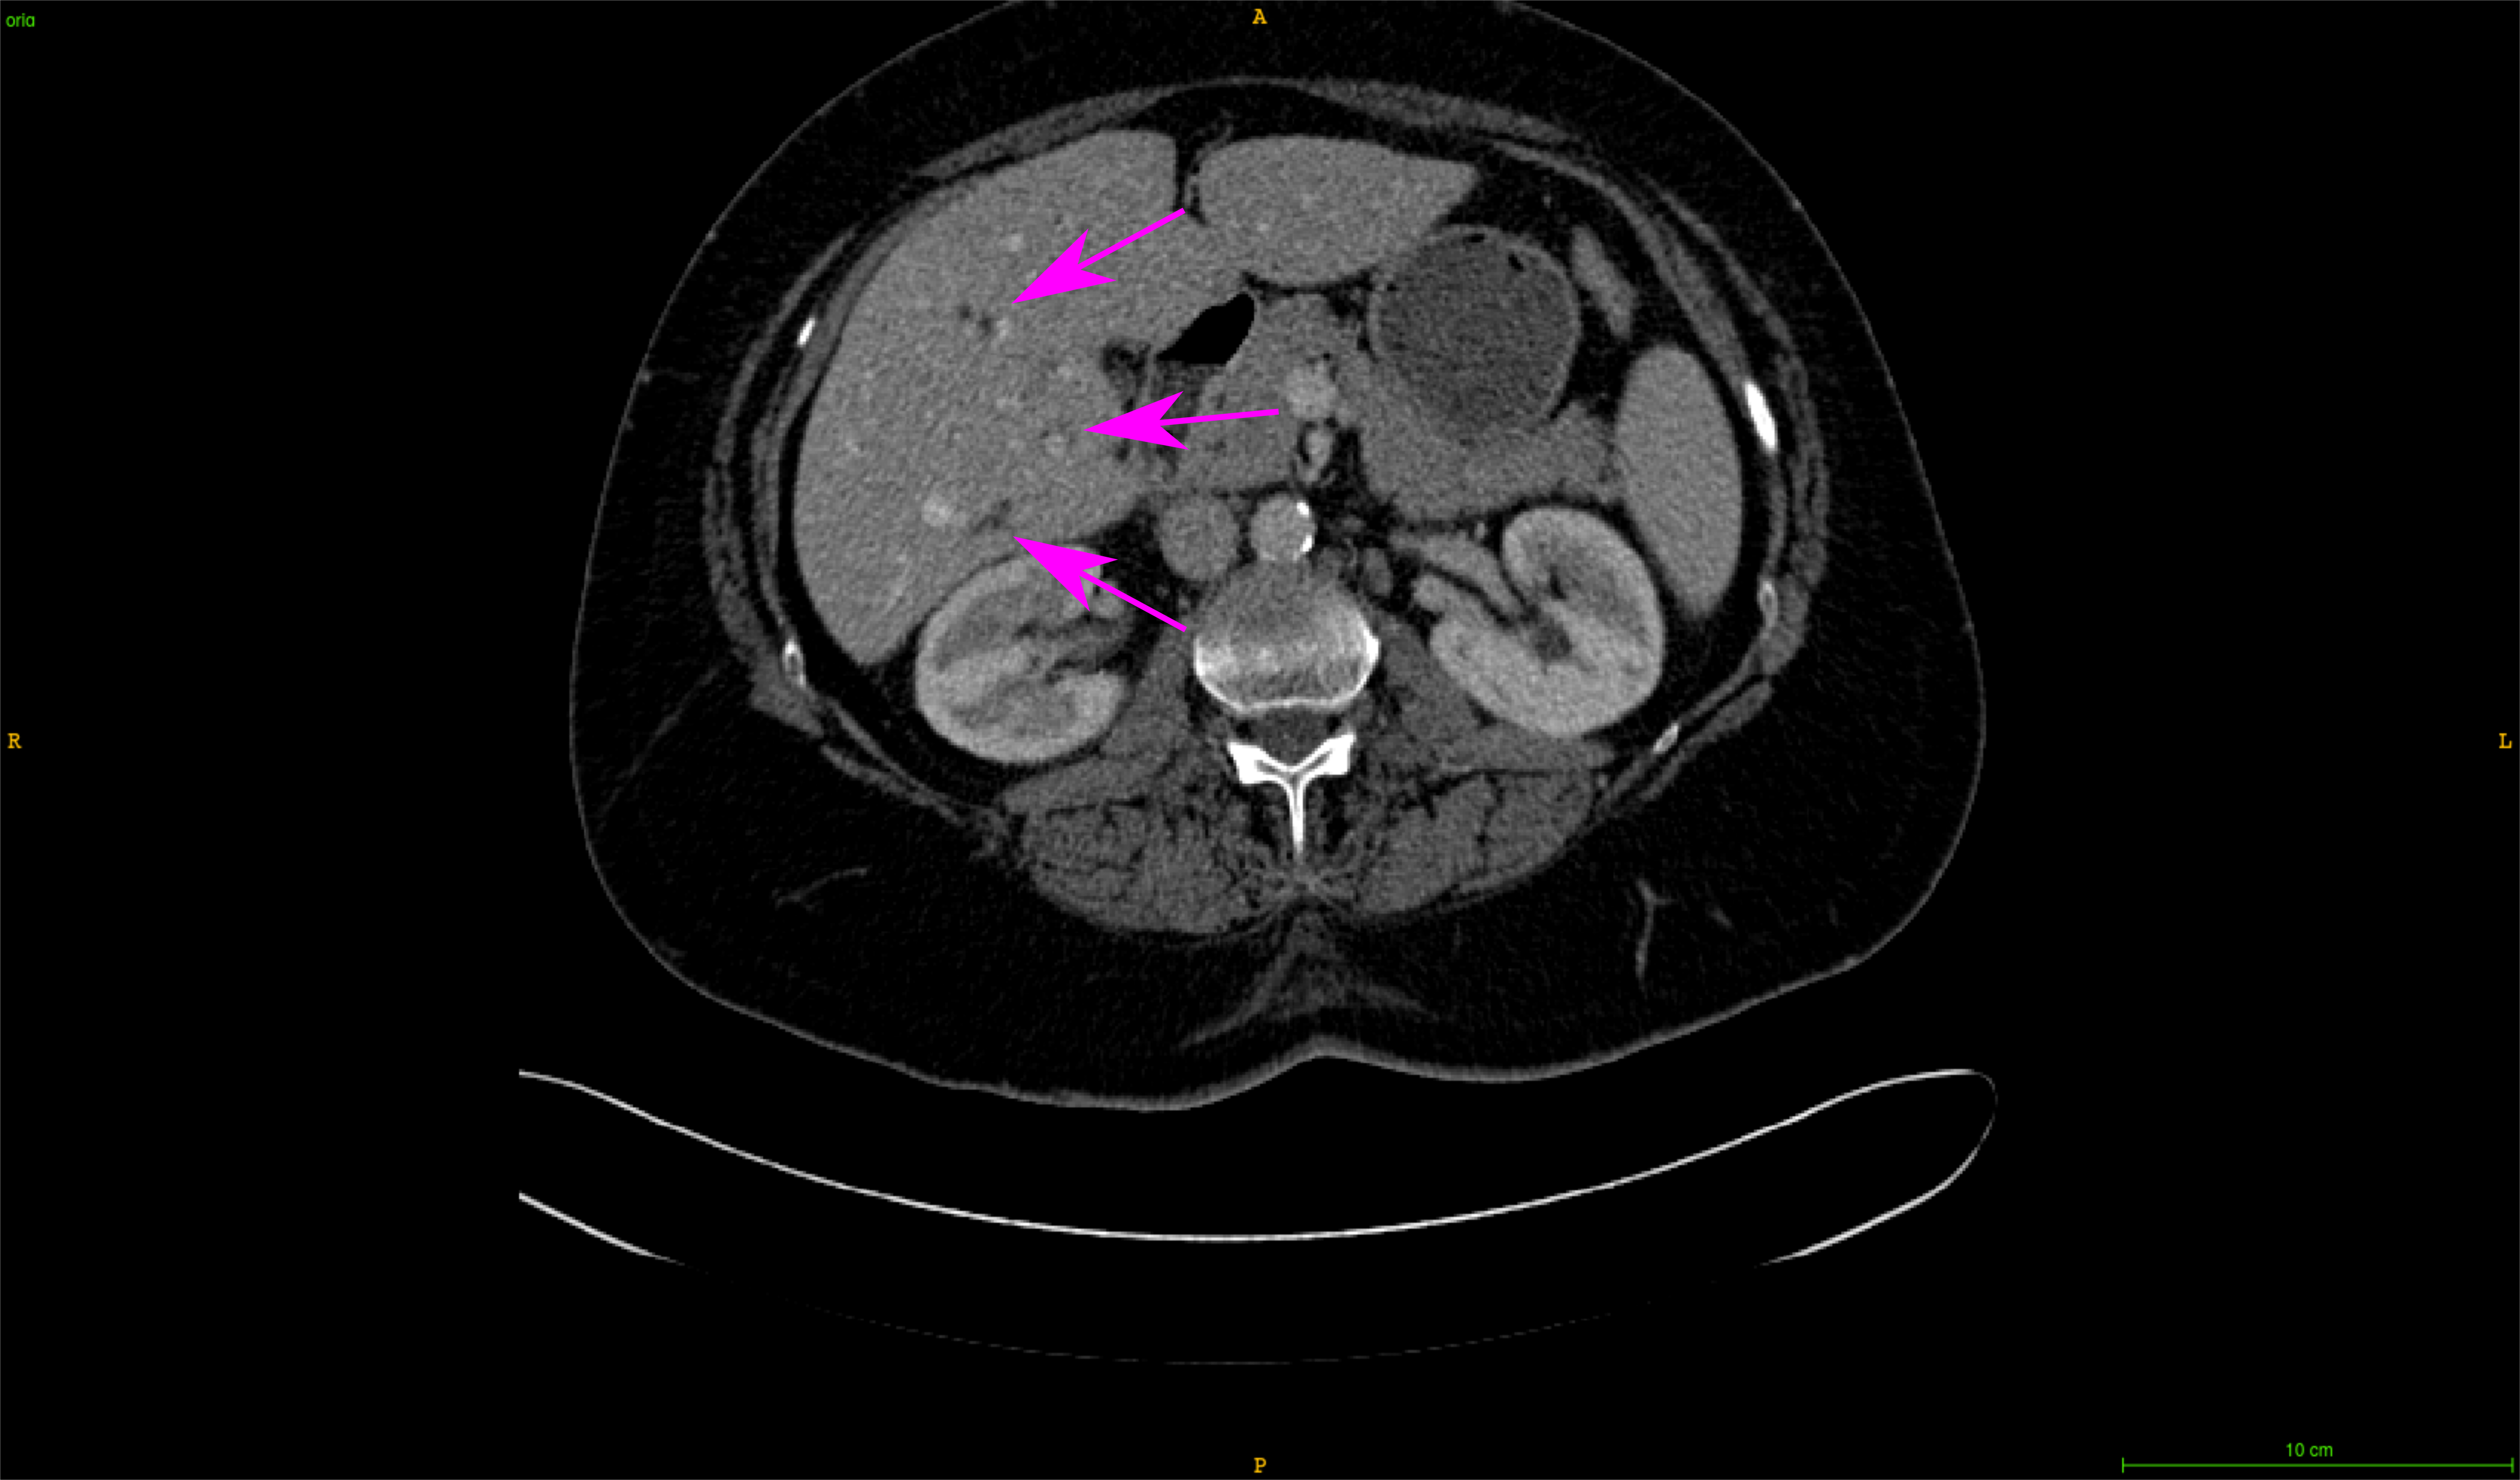
\includegraphics[width=\linewidth]{../Contributions/images/ResizeTCIA_cirrhoticPatientArrows}
	\end{minipage}
	\caption{Example of cirrhotic patients present in both datasets.  Left: \textbf{\lmttfont{LITS-dB}} images, right: \textbf{\lmttfont{TCIA-dB}} images. We can see the irregular shape (cyan arrows) of the liver with signs of atrophy (pink arrows) in both cases.}
	\label{fig:InterDb_diseasedLivers}
\end{figure}

The quantitative analysis aims to prove the existence of cirrhotic patients in both datasets, and allows an inter and intra-phase evaluation, essentially to prove that a liver segmentation network trained using the \textbf{\lmttfont{LITS-dB}} volumes can perform the liver segmentation on both AR and PV volumes. \\
The quantitative analysis has been performed on randomly chosen patients and consisted on the placement of 5 ROIs by the medical expert in the liver parenchyma, the air, the spleen, the bone and the aorta. The aorta was chosen to analyze the changes in terms of contrast agent concentration\footnote{Assuming that the aorta is the best area to measure the concentration of contrast agent}. The liver parenchyma and the spleen were also affected by the contrast agent diffusion, but they were mainly used to diagnose diseased patients since a difference of more than 18.5 HU \footnote{In cirrhotic livers, the portal system is the most affected, to such an extent that the arterial inflow increases, hence the contrast inflow, whereas the spleen is less affected.} between both areas at portal venous phase could be a sign of cirrhosis \cite{Wells2016}. It is worth noting that the ROIs in the liver parenchyma were placed in the peripheral parts of the liver to avoid vessels. The bone and the air ROIs served as control since the air is supposed to have always the same intensity (-1000 HU independently of the acquisition parameters), while the calcium present in the bone renders the circulation of the contrast agent difficult, and this ROI can be used as a way to compare the different phases. An example of annotation is given in the figure \ref{fig:roiPlacement}. \\
The quantitative analysis proved the probable presence of cirrhotic patients in both datasets, as depicted in the figure \ref{fig:cirrhosisPlot}.
\begin{figure}[!ht]
	\centering
	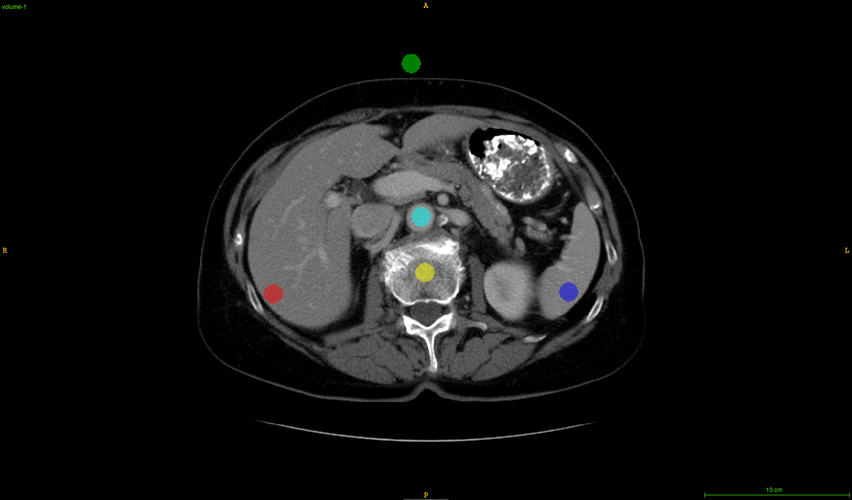
\includegraphics[width=0.6\linewidth]{../Contributions/images/Resizejuan_Roi_Example}
	\caption{Example of ROI placement for the quantitative evaluation of differences between the \textbf{\lmttfont{LITS-dB}} and the \textbf{\lmttfont{TCIA-dB}}. Red: liver parenchyma, green: air, blue: spleen, yellow: bone, cyan: aorta.}
	\label{fig:roiPlacement}
\end{figure}
\begin{figure}[!ht]
	\centering
	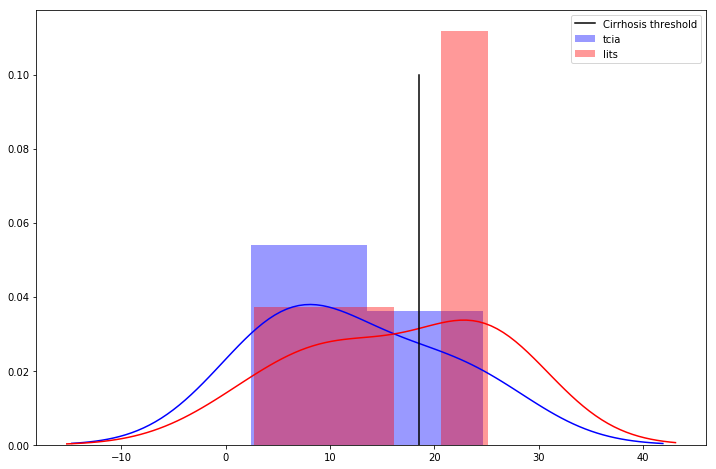
\includegraphics[width=0.6\linewidth]{../Contributions/images/LITS_TCIA_cirrhosisPlot}
	\caption{Histogram representing the distribution of the difference between parenchyma and spleen intensities, where a difference higher than 18.5 HU (black vertical line) can be a sign of cirrhosis.}
	\label{fig:cirrhosisPlot}
\end{figure}


Finally, regarding the available contrast-enhanced phases per dataset, it has been proved that \textbf{\lmttfont{LITS-dB}} contains volumes that can be labeled as arterial and some other that can be labeled as portal venous (see figure \ref{fig:LitsTciaPhasePlot}).
\begin{figure}[!ht]
	\centering
	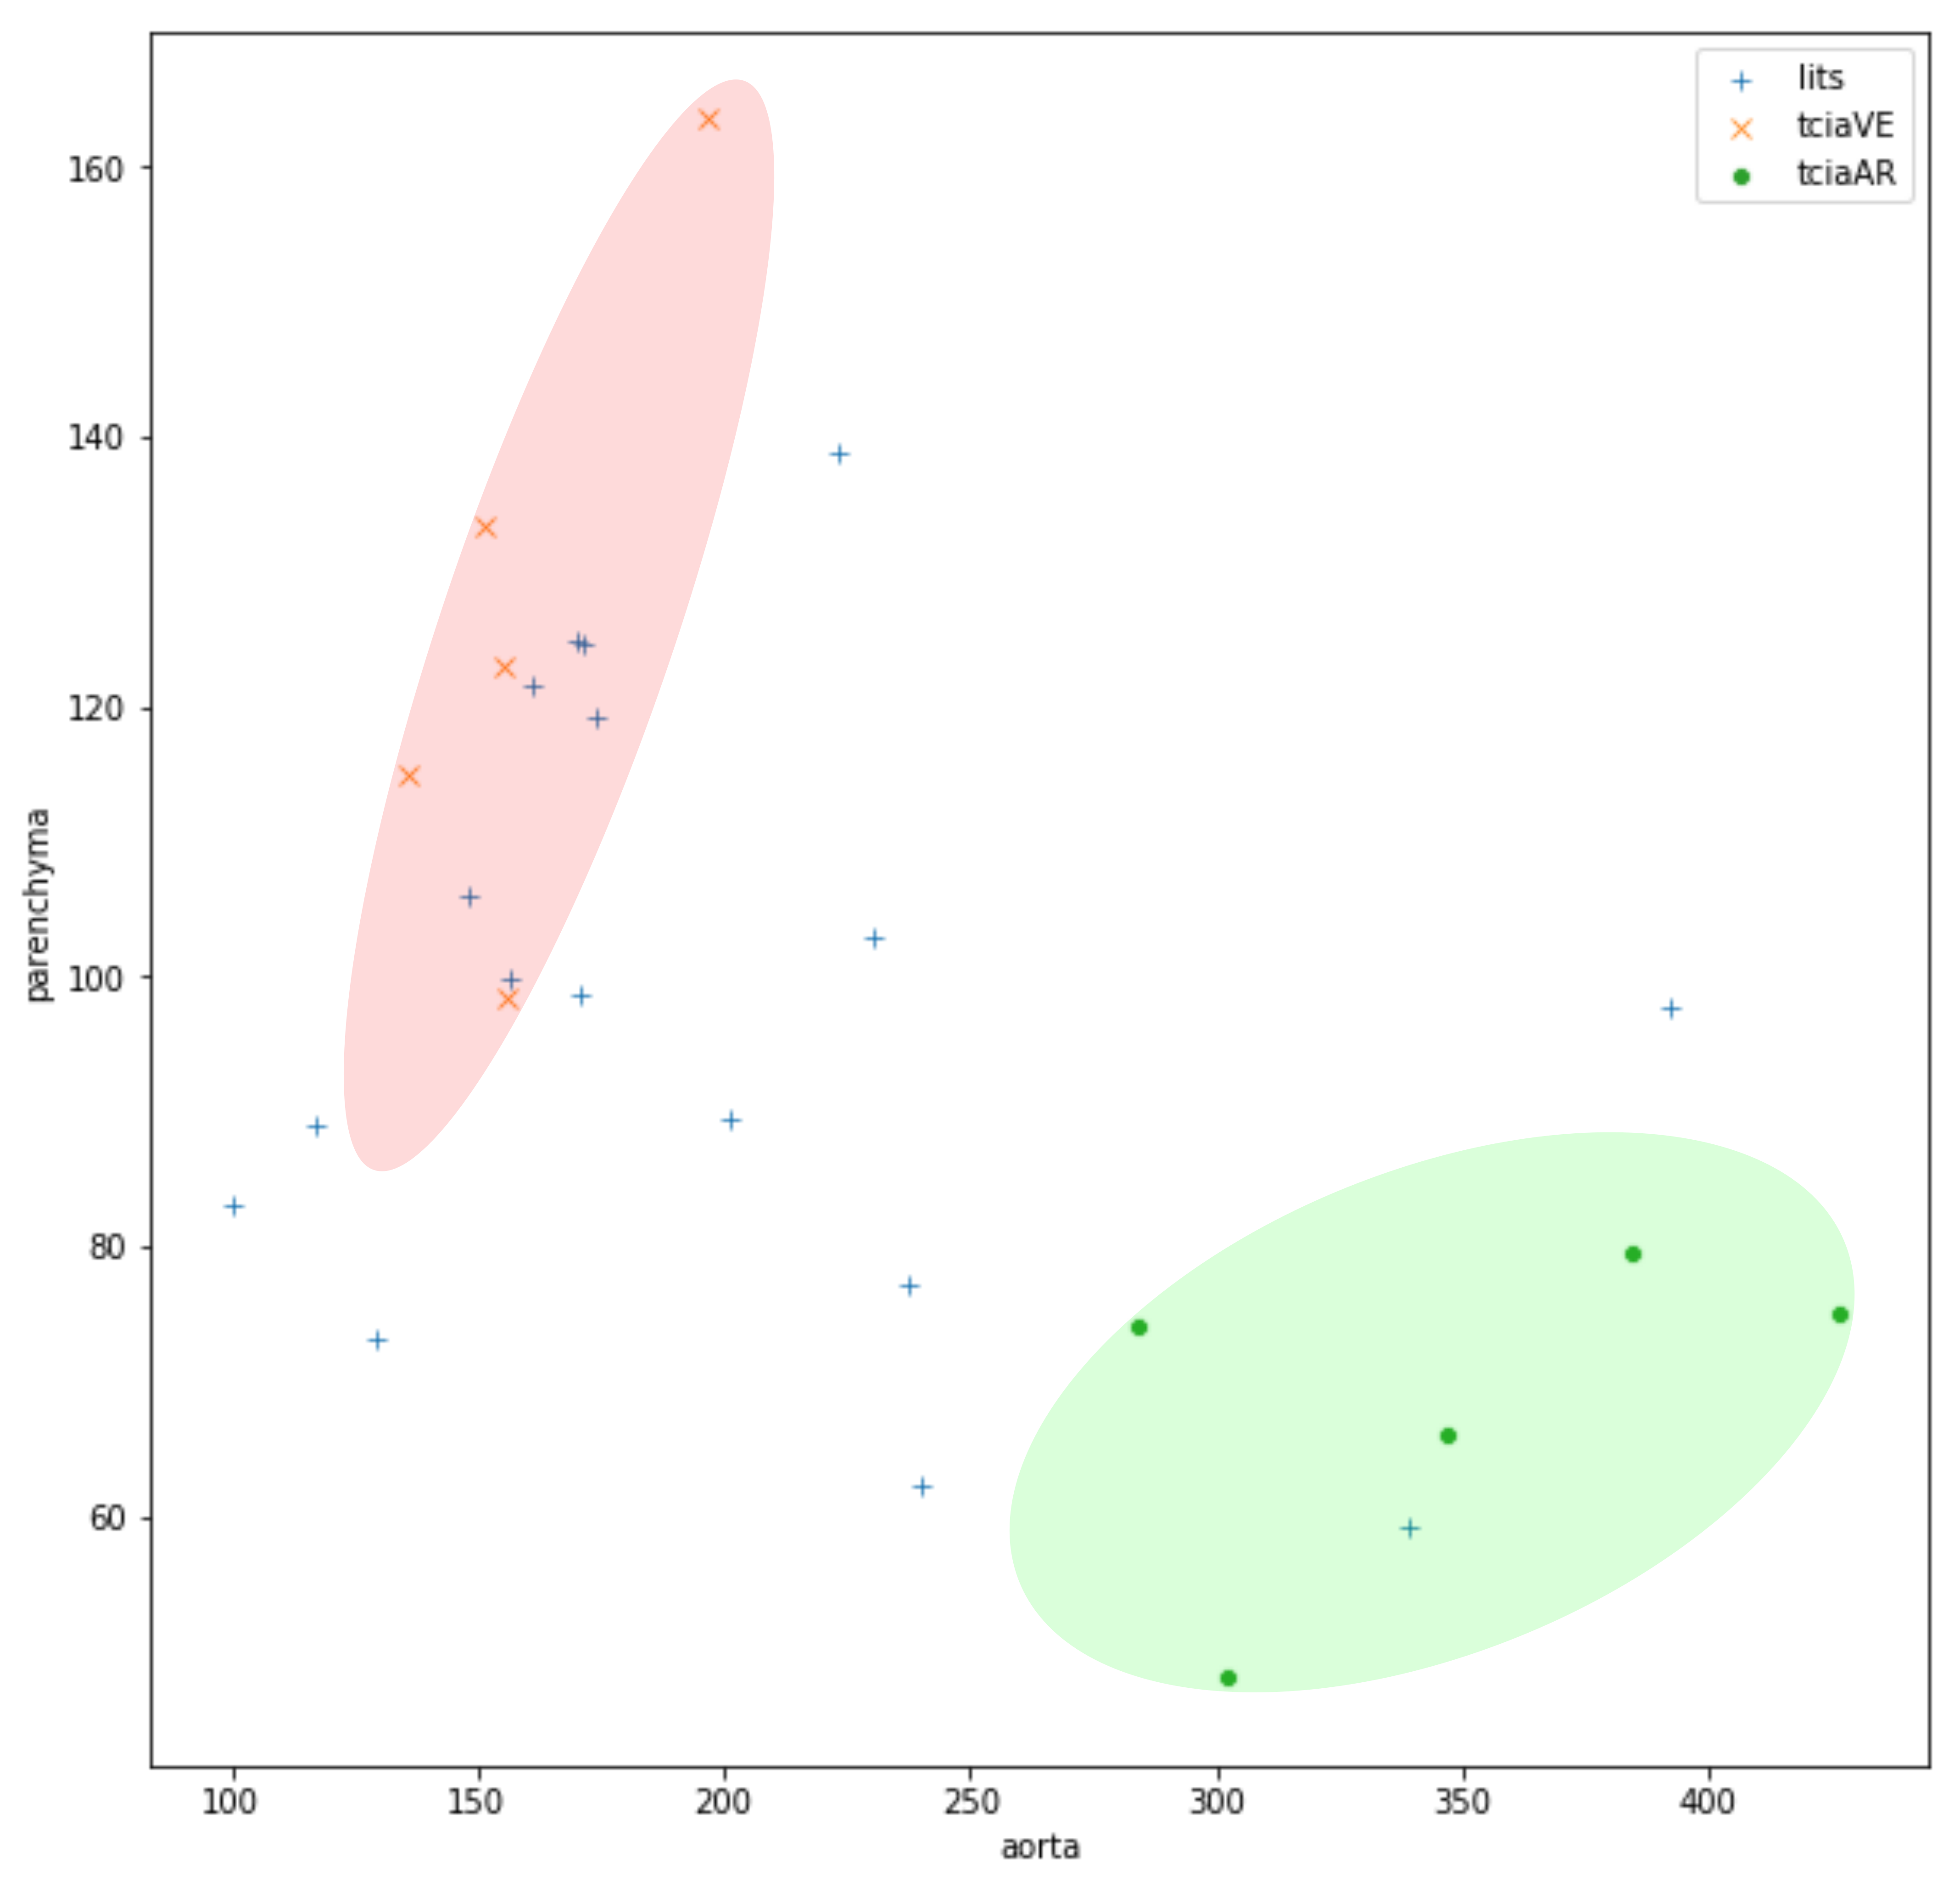
\includegraphics[width=0.6\linewidth]{../Contributions/images/AortaParPlot}
	\caption{Mean aorta intensity vs mean liver parenchyma intensity. Each point represents one volume. We can see a clear separation between arterial (green dots) and portal venous (red crosses) volumes among the \textbf{\lmttfont{TCIA-dB}} patients. Portal venous volumes present a higher variance for their liver parenchyma intensities, which can be explained by the differences in terms of duration between the injection of contrast medium and the acquisition of the images. It seems clear that the majority of volumes from the \textbf{\lmttfont{LITS-dB}} were acquired during the portal venous phase whereas some of them were acquired during the arterial phase. The rest of the volumes can be classified as belonging to the late arterial or the early portal venous phase.
	}
	\label{fig:LitsTciaPhasePlot}
\end{figure}
Since all the patients of the \textbf{\lmttfont{TCIA-dB}} were supposed to be affected by HCC, it would have been ideal to train our liver segmentation network with a dataset only composed of patients suffering from HCC (or by a large solitary tumor), but only 20 patients of the 131 from the \textbf{\lmttfont{LITS-dB}} were affected by a single lesion larger than $ 2cm^3 $.
Since we considered that the type of lesions will only slightly affect the liver segmentation, we decided to keep all the patients of the \textbf{\lmttfont{LITS-dB}} (independently of the number of lesions present in the liver) to train our liver segmentation network.
Moreover, it would have been optimal to train one network per injected phase, or a single network with multiphase images as input.
However \textbf{\lmttfont{LITS-dB}} being composed of both \ac{ar} and \ac{pv} volumes (with in-between phase volumes as depicted in the figure \ref{fig:LitsTciaPhasePlot}), we used the entire dataset to train a single network, allowing us to segment the liver on both \ac{ar} and \ac{pv} volumes independently.


\subsection{Liver tumor segmentation inter-dataset comparison (\textbf{\lmttfont{G-dB}} vs \textbf{\lmttfont{TCIA-dB}})} \label{liver_tumor_interdb_comparison}


We also compared both the training (\textbf{\lmttfont{G-dB}}) and the testing (\textbf{\lmttfont{TCIA-dB}}) datasets used for the liver tumor segmentation task using the same analysis as the one performed previously (see section \ref{liver_interdb_comparison}).
Therefore, a medical expert was asked to evaluate both visually and quantitatively the differences between the two datasets.
To perform the visual examination, he was asked to evaluate the type of characteristics present in both datasets, not only in the liver but also by comparing the tumors using imaging features. 
As exposed previously, \textbf{\lmttfont{TCIA-dB}} contains both large and small tumors. The same panel of tumor sizes was present in the \textbf{\lmttfont{G-dB}} dataset, as illustrated in the figure \ref{fig:interdb_tumorSeg_tumorExamples}.

Some artifacts were also found in the \textbf{\lmttfont{G-dB}} dataset, such as the presence of benign lesions, fat accumulation or other metallic artifacts in the hepatic region (see figure \ref{fig:GDb_artifacts}).
As it was the case in the \textbf{\lmttfont{TCIA-dB}} dataset, diseased livers were also present among the \textbf{\lmttfont{G-dB}} patients, as illustrated in the figure \ref{fig:GDb_diseasedLivers}.
Regarding the tumor specific area, several imaging features were found in both datasets:
\begin{itemize}
\item the presence of internal arteries
\item a peritumoral enhancement
\item the presence of either smooth or non-smooth margins
\item an hypoattenuating halo surrounding the tumor
\item a high textural heterogeneity
\item a wash-in/wash-out pattern 
\end{itemize}
Images illustrated each of the above mentioned features were given in the figure \ref{fig:InterDb_imagingTraits}.

\begin{figure}[!ht]
	\centering
	\begin{minipage}{0.45\linewidth}
		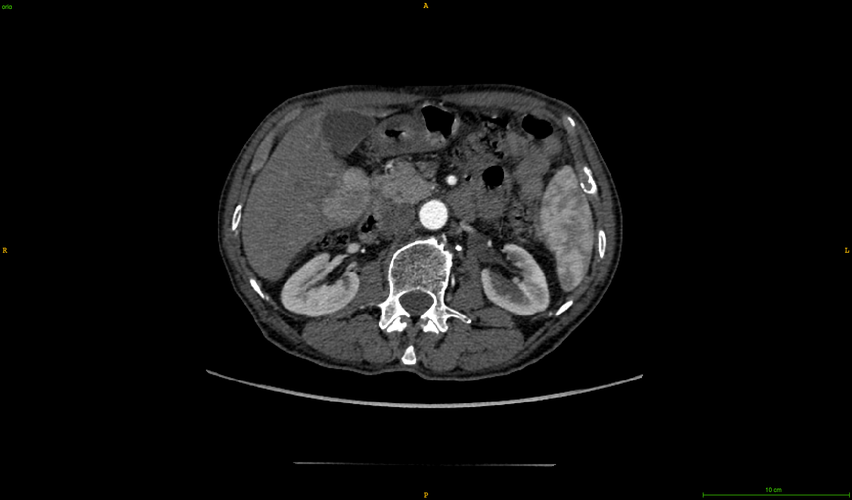
\includegraphics[width=\linewidth]{../Contributions/images/ResizeGDB_examplePatientSmallTumor}
	\end{minipage} \hspace{-0.1cm}
	\begin{minipage}{0.45\linewidth}
		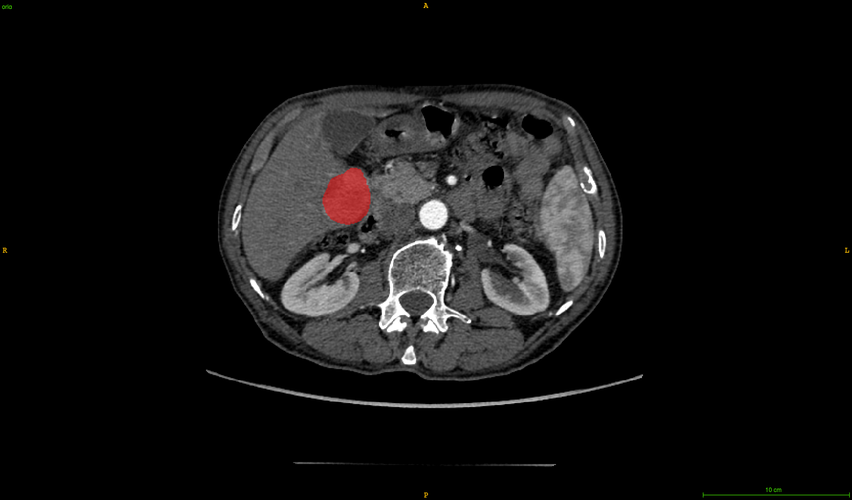
\includegraphics[width=\linewidth]{../Contributions/images/ResizeGDB_examplePatientSmallTumor_seg}
	\end{minipage} \\
	\begin{minipage}{0.45\linewidth}
		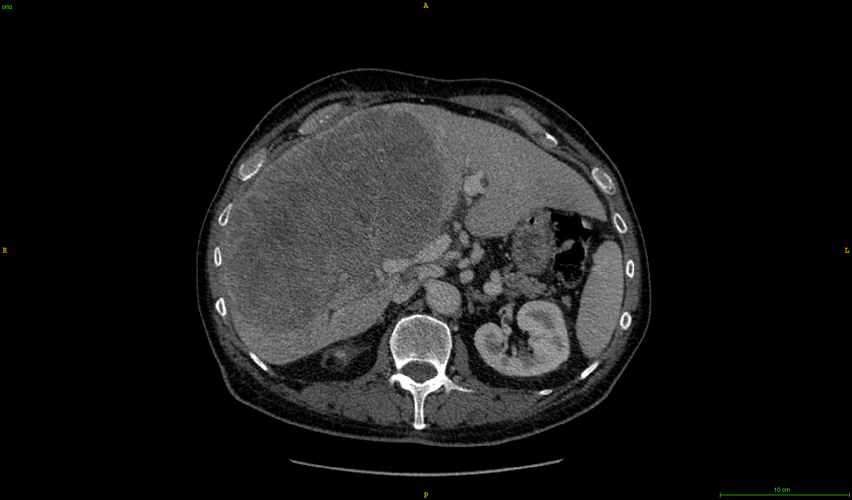
\includegraphics[width=\linewidth]{../Contributions/images/ResizeGDB_examplePatientLargeTumor}
	\end{minipage} \hspace{-0.1cm}
	\begin{minipage}{0.45\linewidth}
		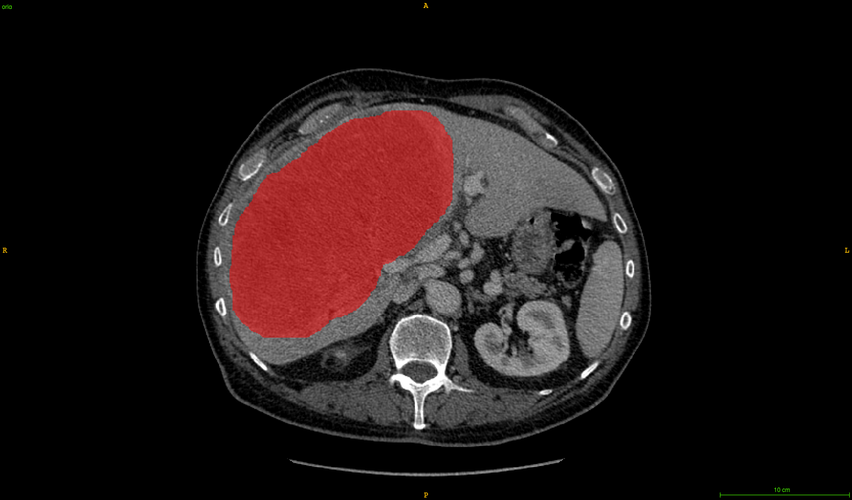
\includegraphics[width=\linewidth]{../Contributions/images/ResizeGDB_examplePatientLargeTumor_seg}
	\end{minipage}
	\caption{Example of small and large tumors from the \textbf{\lmttfont{G-dB}} images, top: small tumors, bottom: large tumors, left: raw image, left: expert segmentation.}
	\label{fig:interdb_tumorSeg_tumorExamples}
\end{figure}
\begin{figure}[!ht]
	\centering
	\begin{minipage}{0.45\linewidth}
		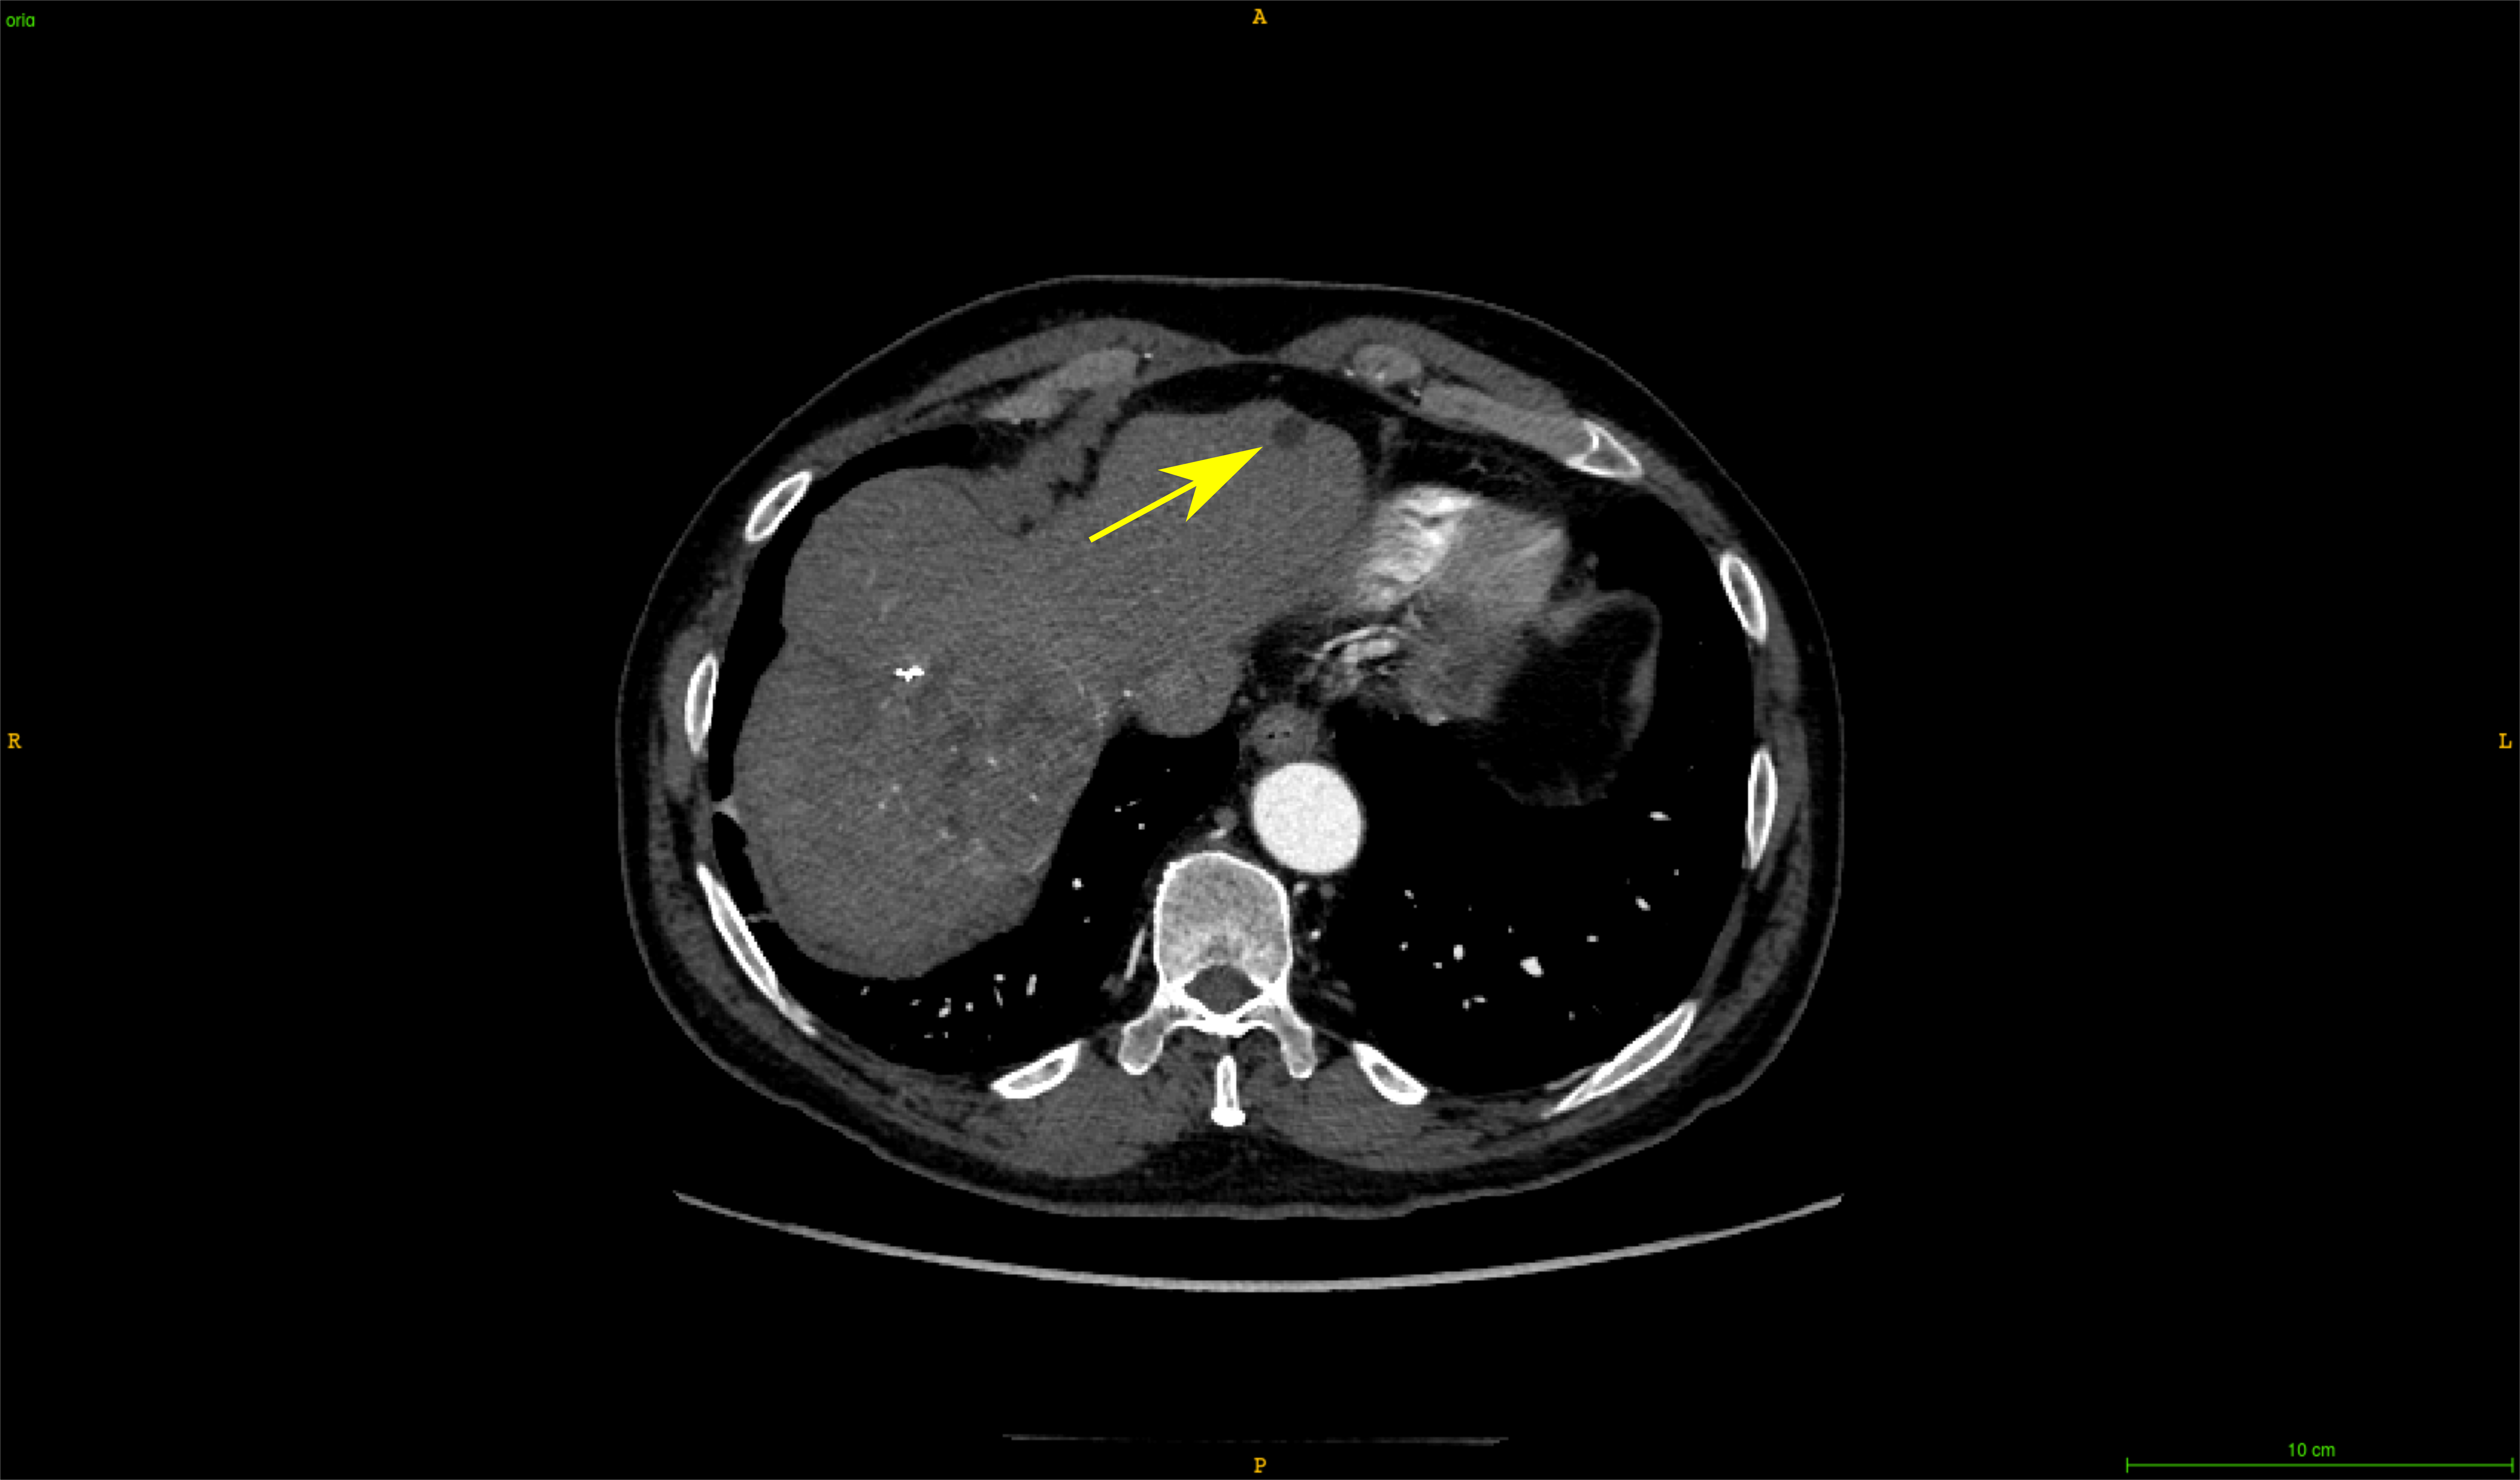
\includegraphics[width=\linewidth]{../Contributions/images/Artifacts/ResizeGDB_cyst}
	\end{minipage} \\
	\begin{minipage}{0.45\linewidth}
		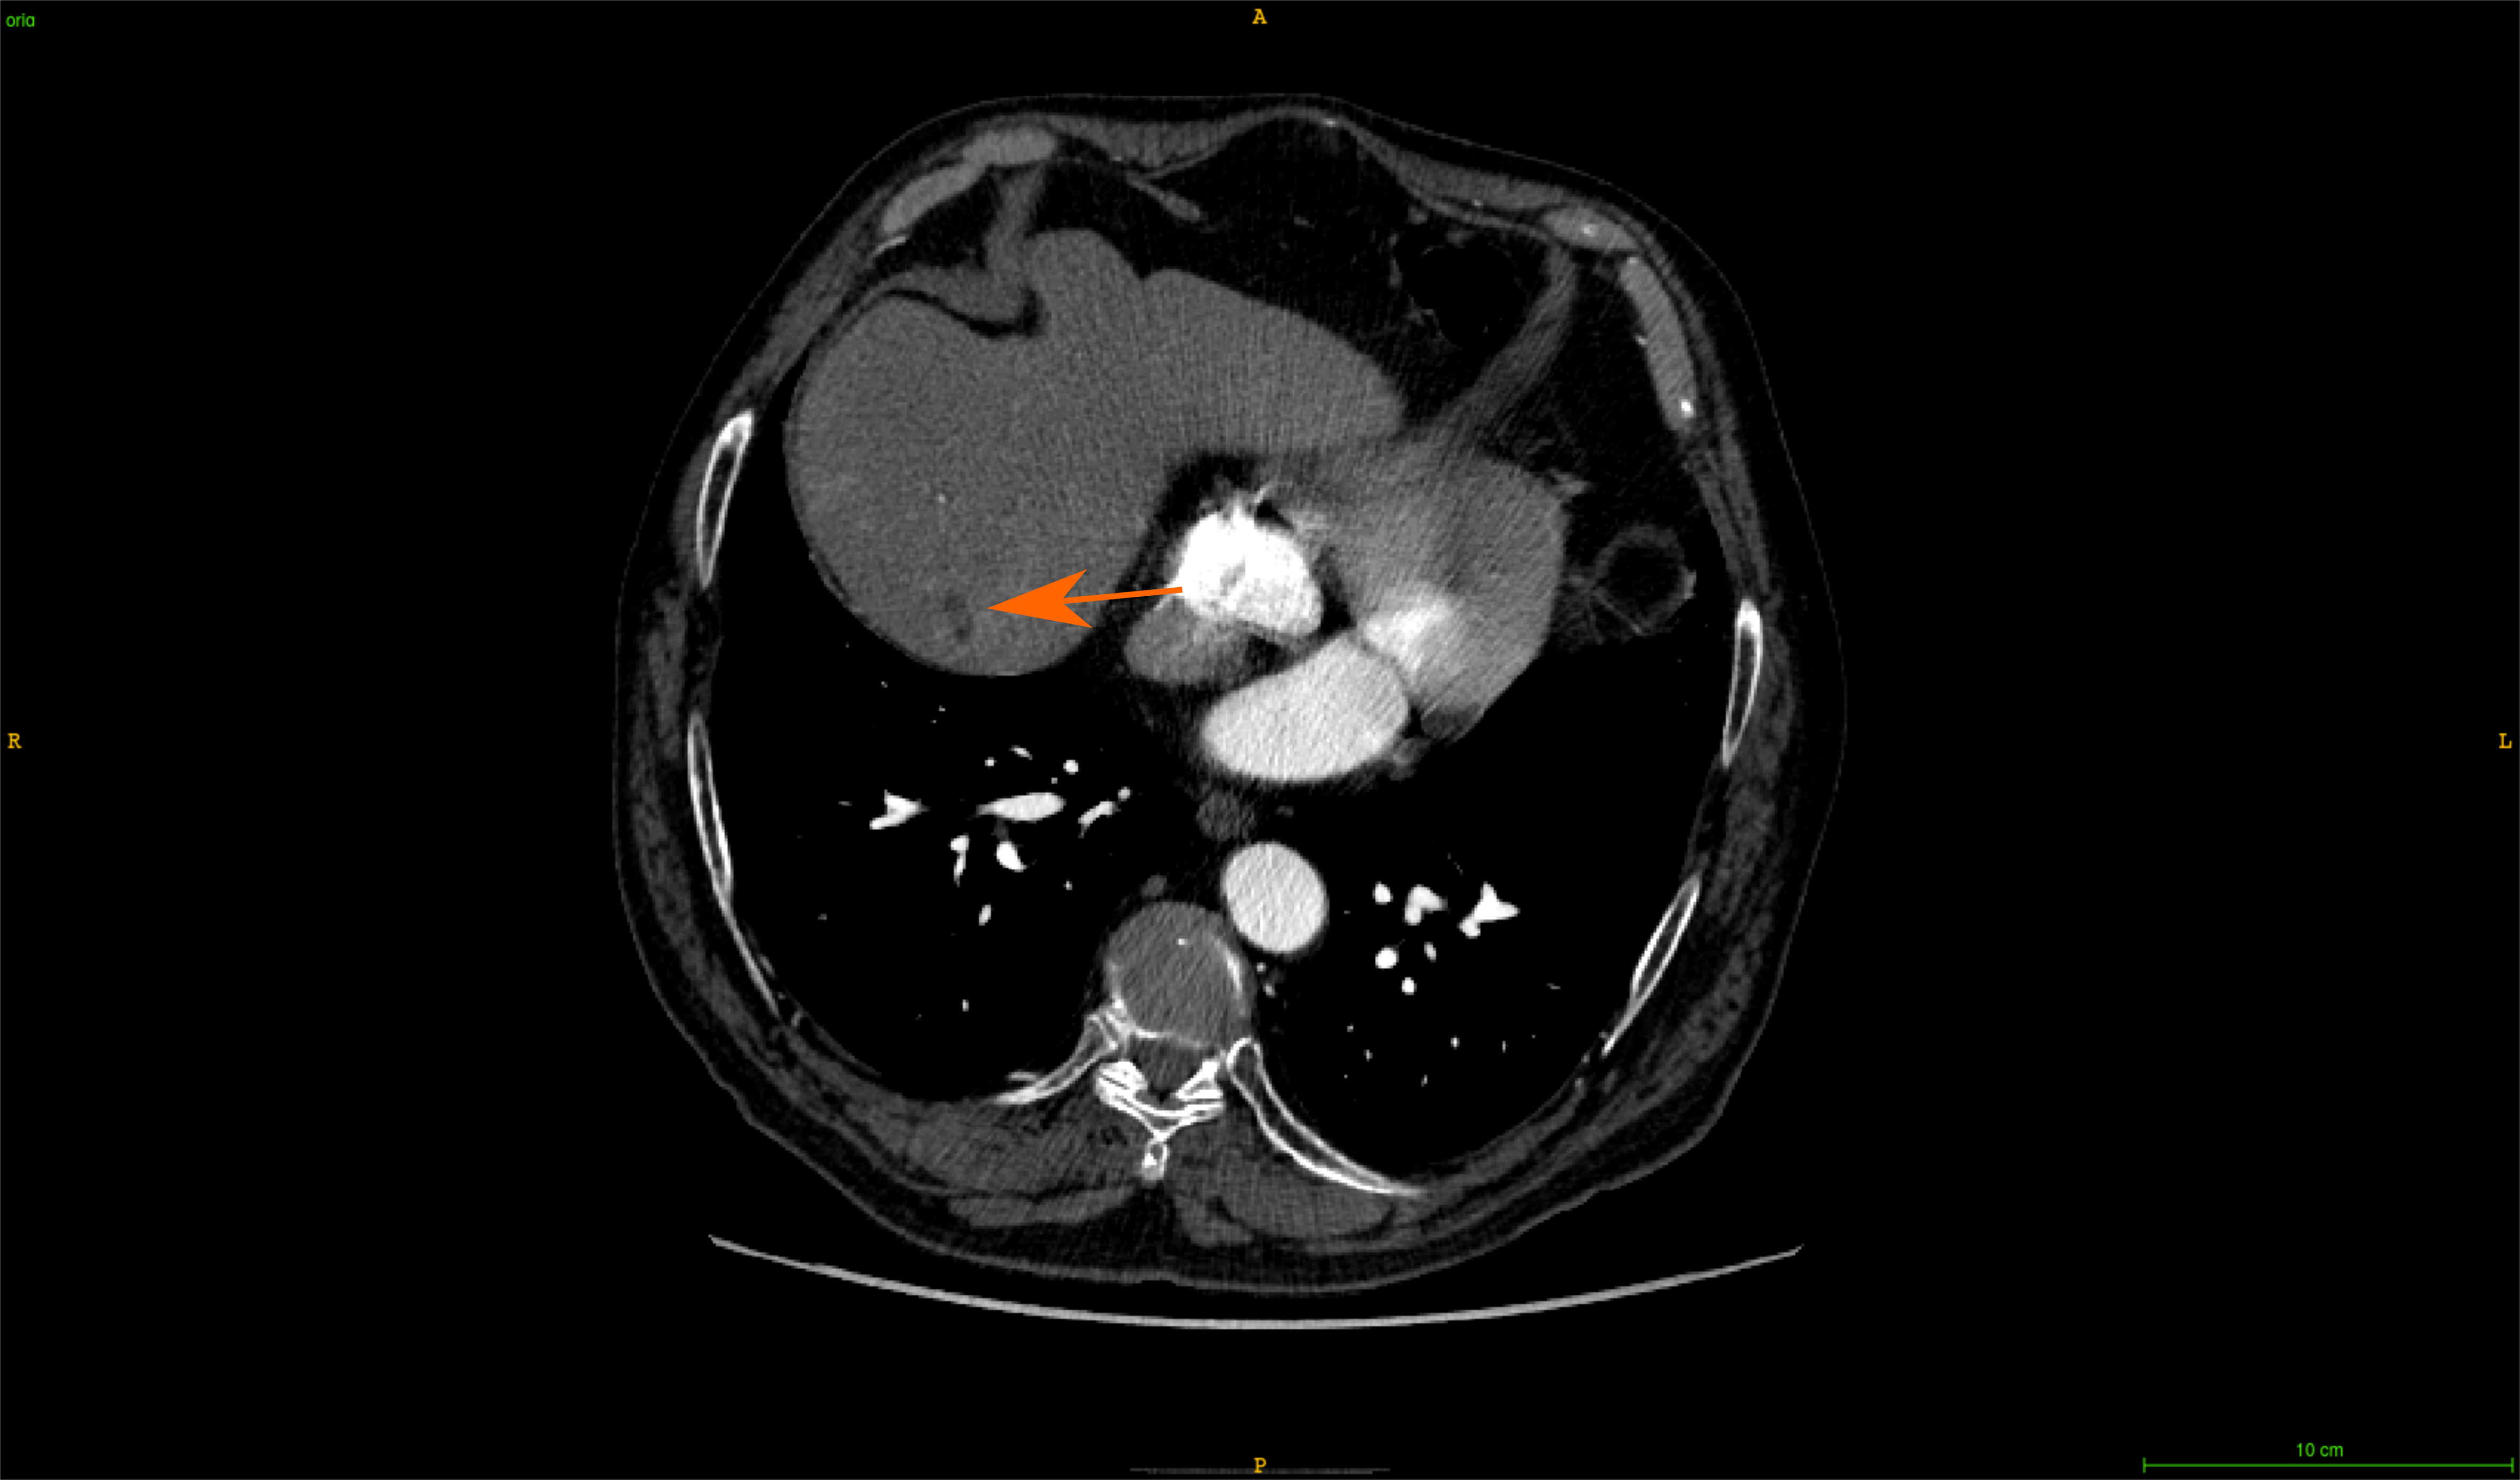
\includegraphics[width=\linewidth]{../Contributions/images/Artifacts/ResizeGDB_fat}
	\end{minipage} \\
	\begin{minipage}{0.45\linewidth}
		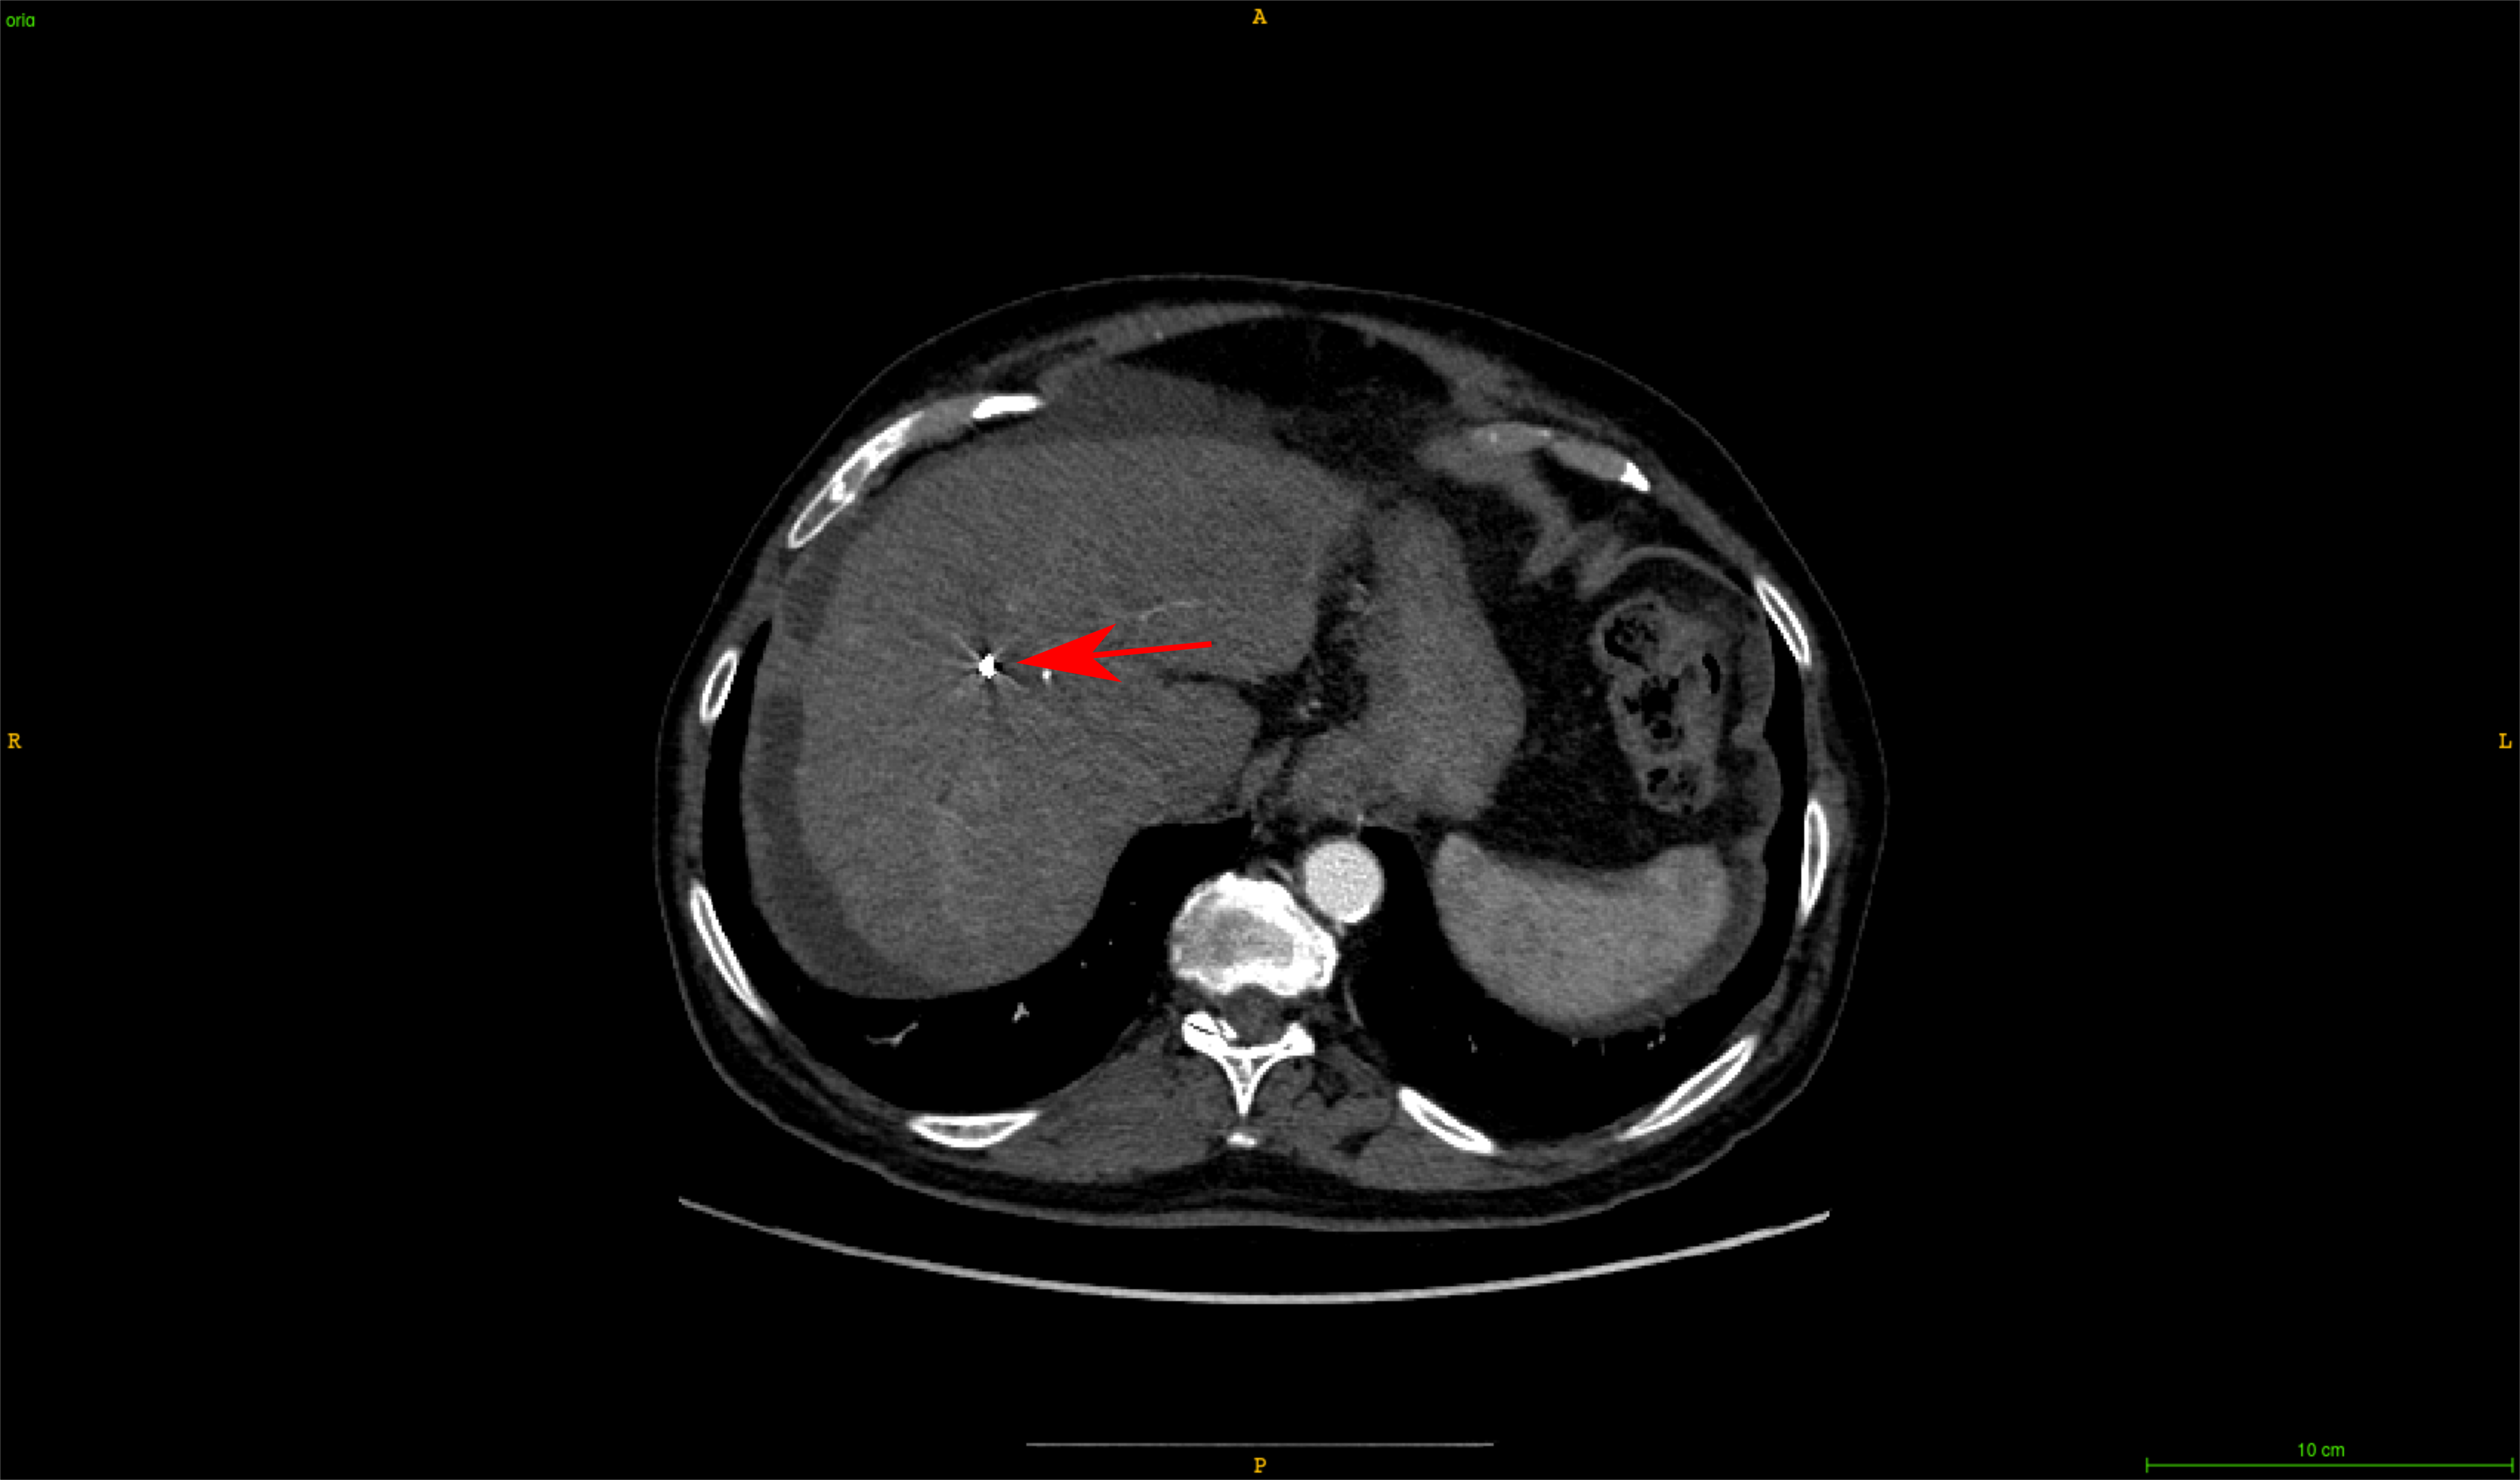
\includegraphics[width=\linewidth]{../Contributions/images/Artifacts/ResizeGDB_metallic_artifacts}
	\end{minipage}
	\caption{Example of artifacts present in the \textbf{\lmttfont{G-dB}} dataset. First row depicts a patient with benign hepatic lesion (yellow arrow), the second row presents liver with tracks of fat accumulation (orange arrow), whereas the last row gives examples of images with presence of metallic artifacts (red arrow).}
	\label{fig:GDb_artifacts}
\end{figure}
\begin{figure}[!ht]
	\centering
	\begin{minipage}{0.45\linewidth}
		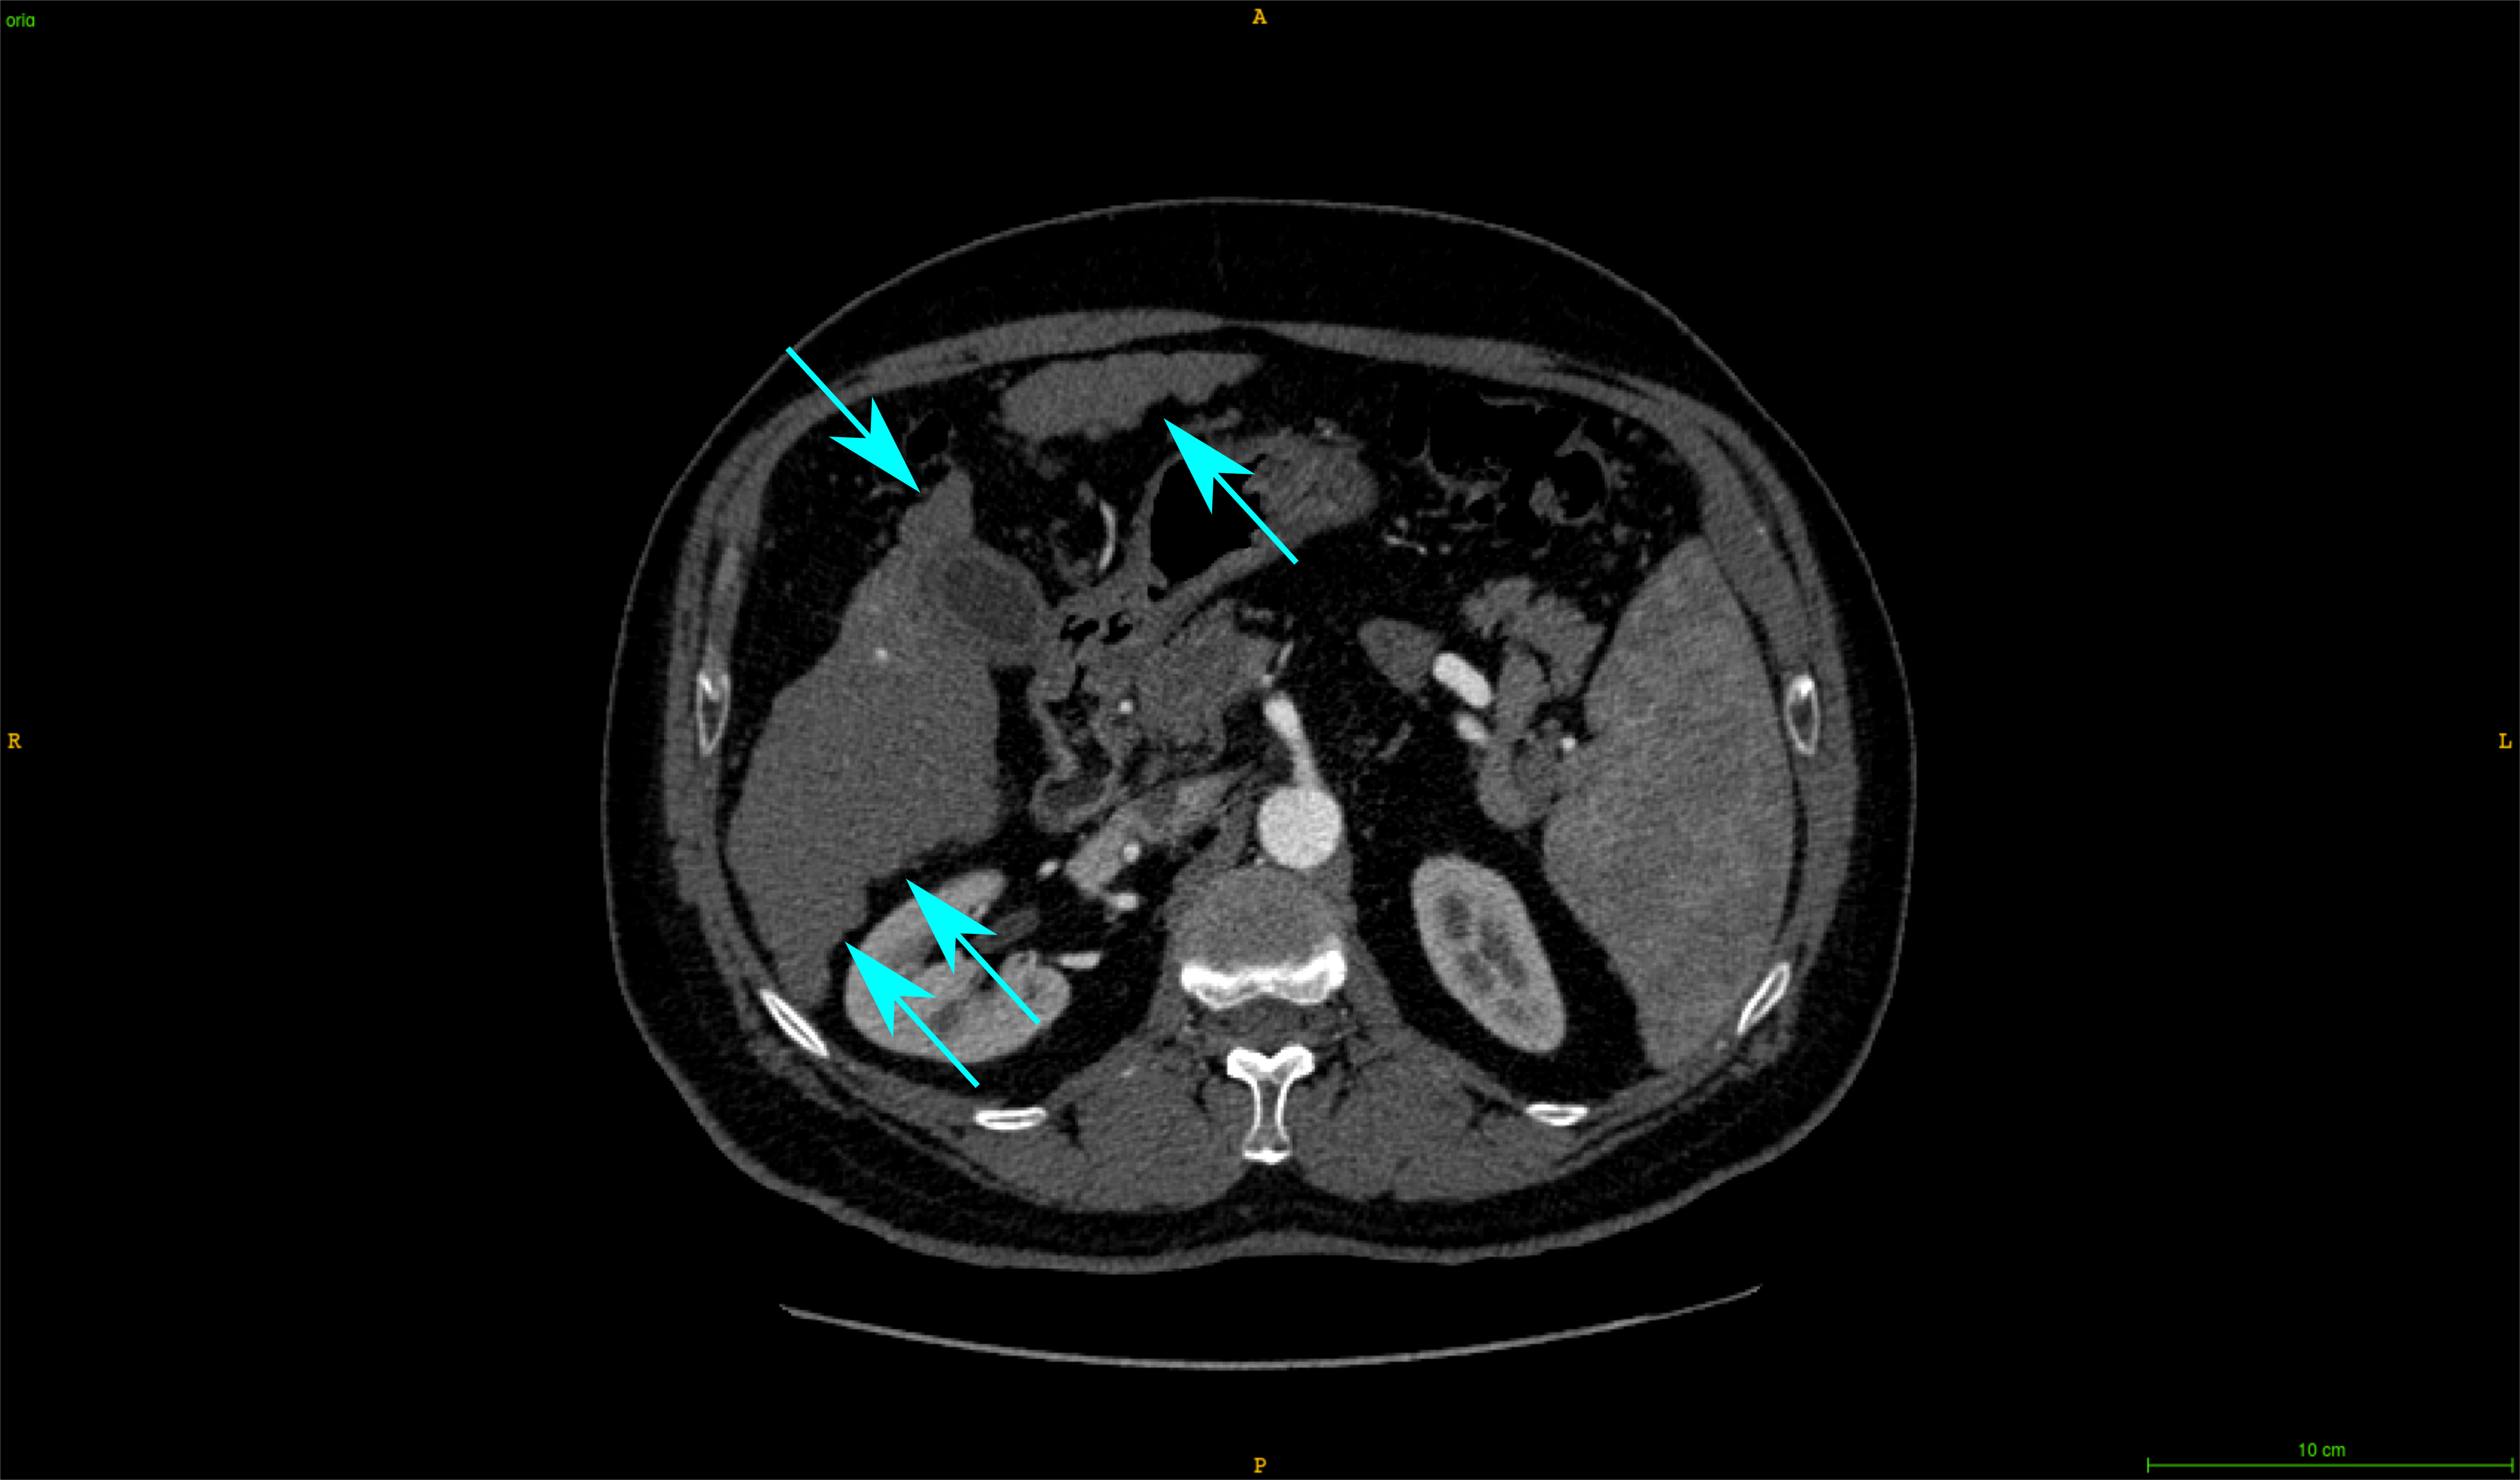
\includegraphics[width=\linewidth]{../Contributions/images/ResizeGDB_cirrhoticPatientArrows}
	\end{minipage} \hspace{-0.1cm}
	\begin{minipage}{0.45\linewidth}
		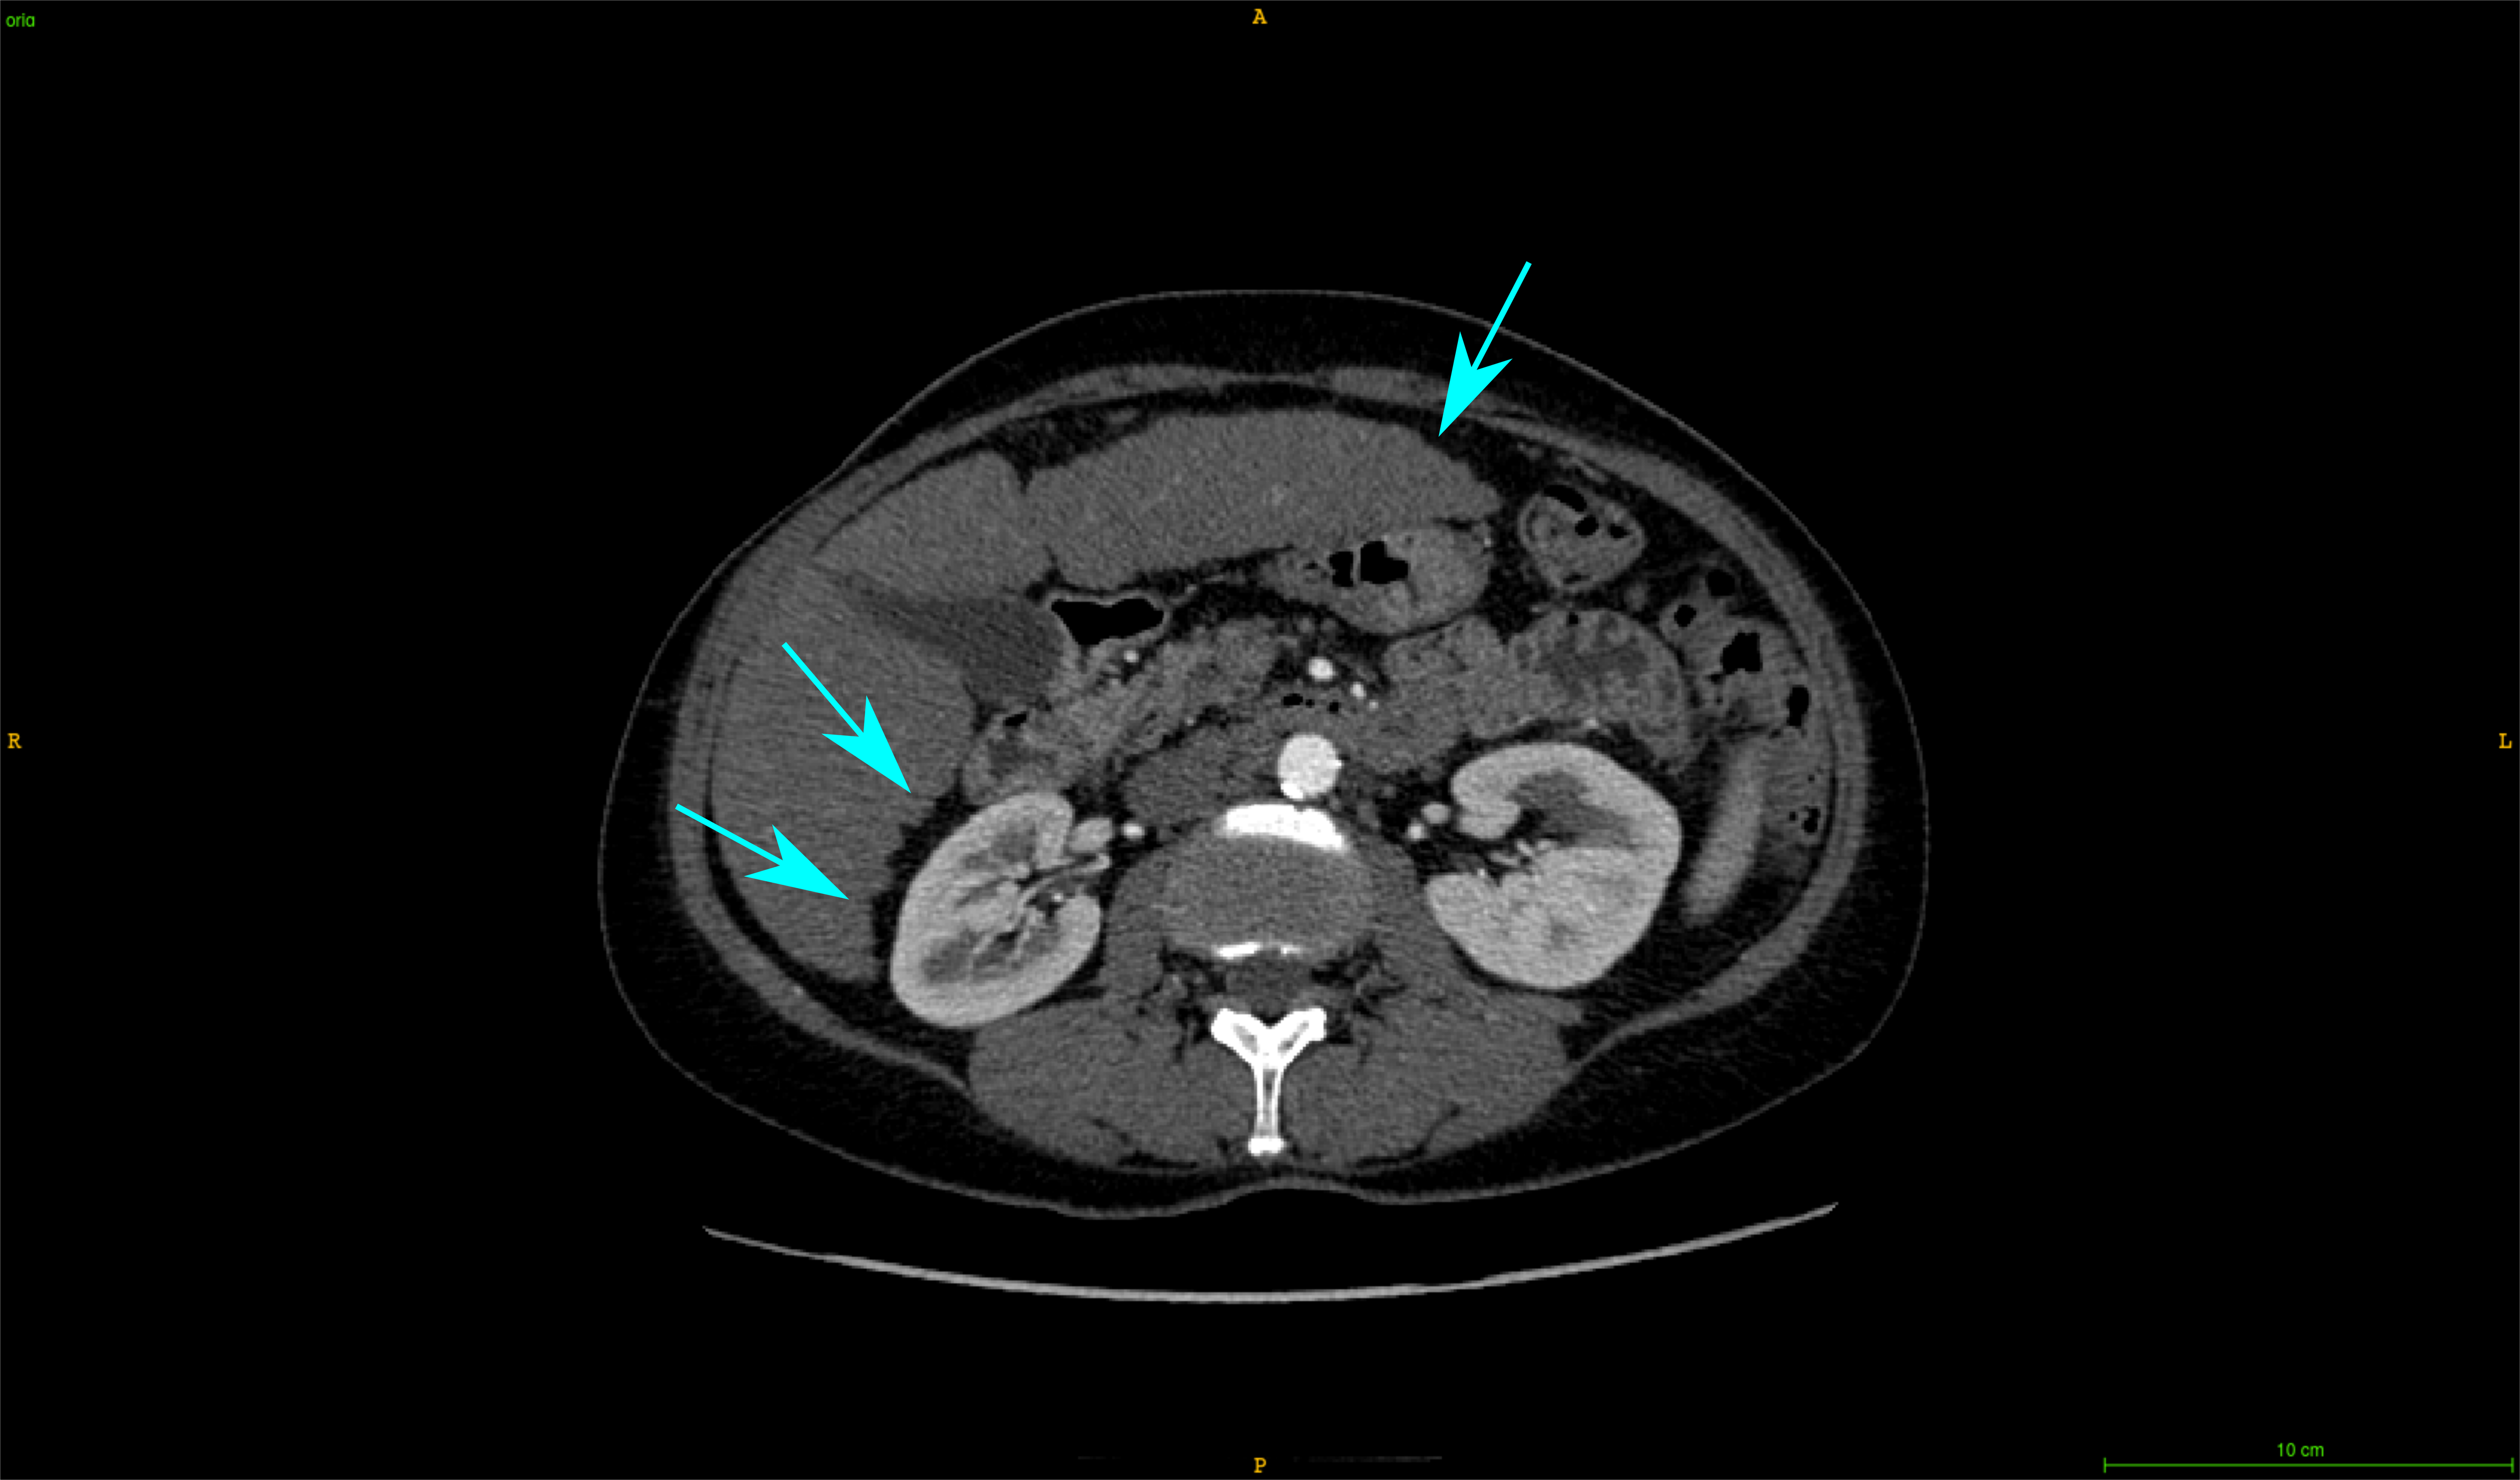
\includegraphics[width=\linewidth]{../Contributions/images/ResizeGDB_cirrhoticPatientArrows_2}
	\end{minipage}
	\caption{Example of cirrhotic patients present in the \textbf{\lmttfont{LITS-dB}} dataset. In both images, we can see the irregular shape (cyan arrows) of the liver.}
	\label{fig:GDb_diseasedLivers}
\end{figure}
\begin{figure}[!ht]
	\centering
	\begin{minipage}{0.45\linewidth}
		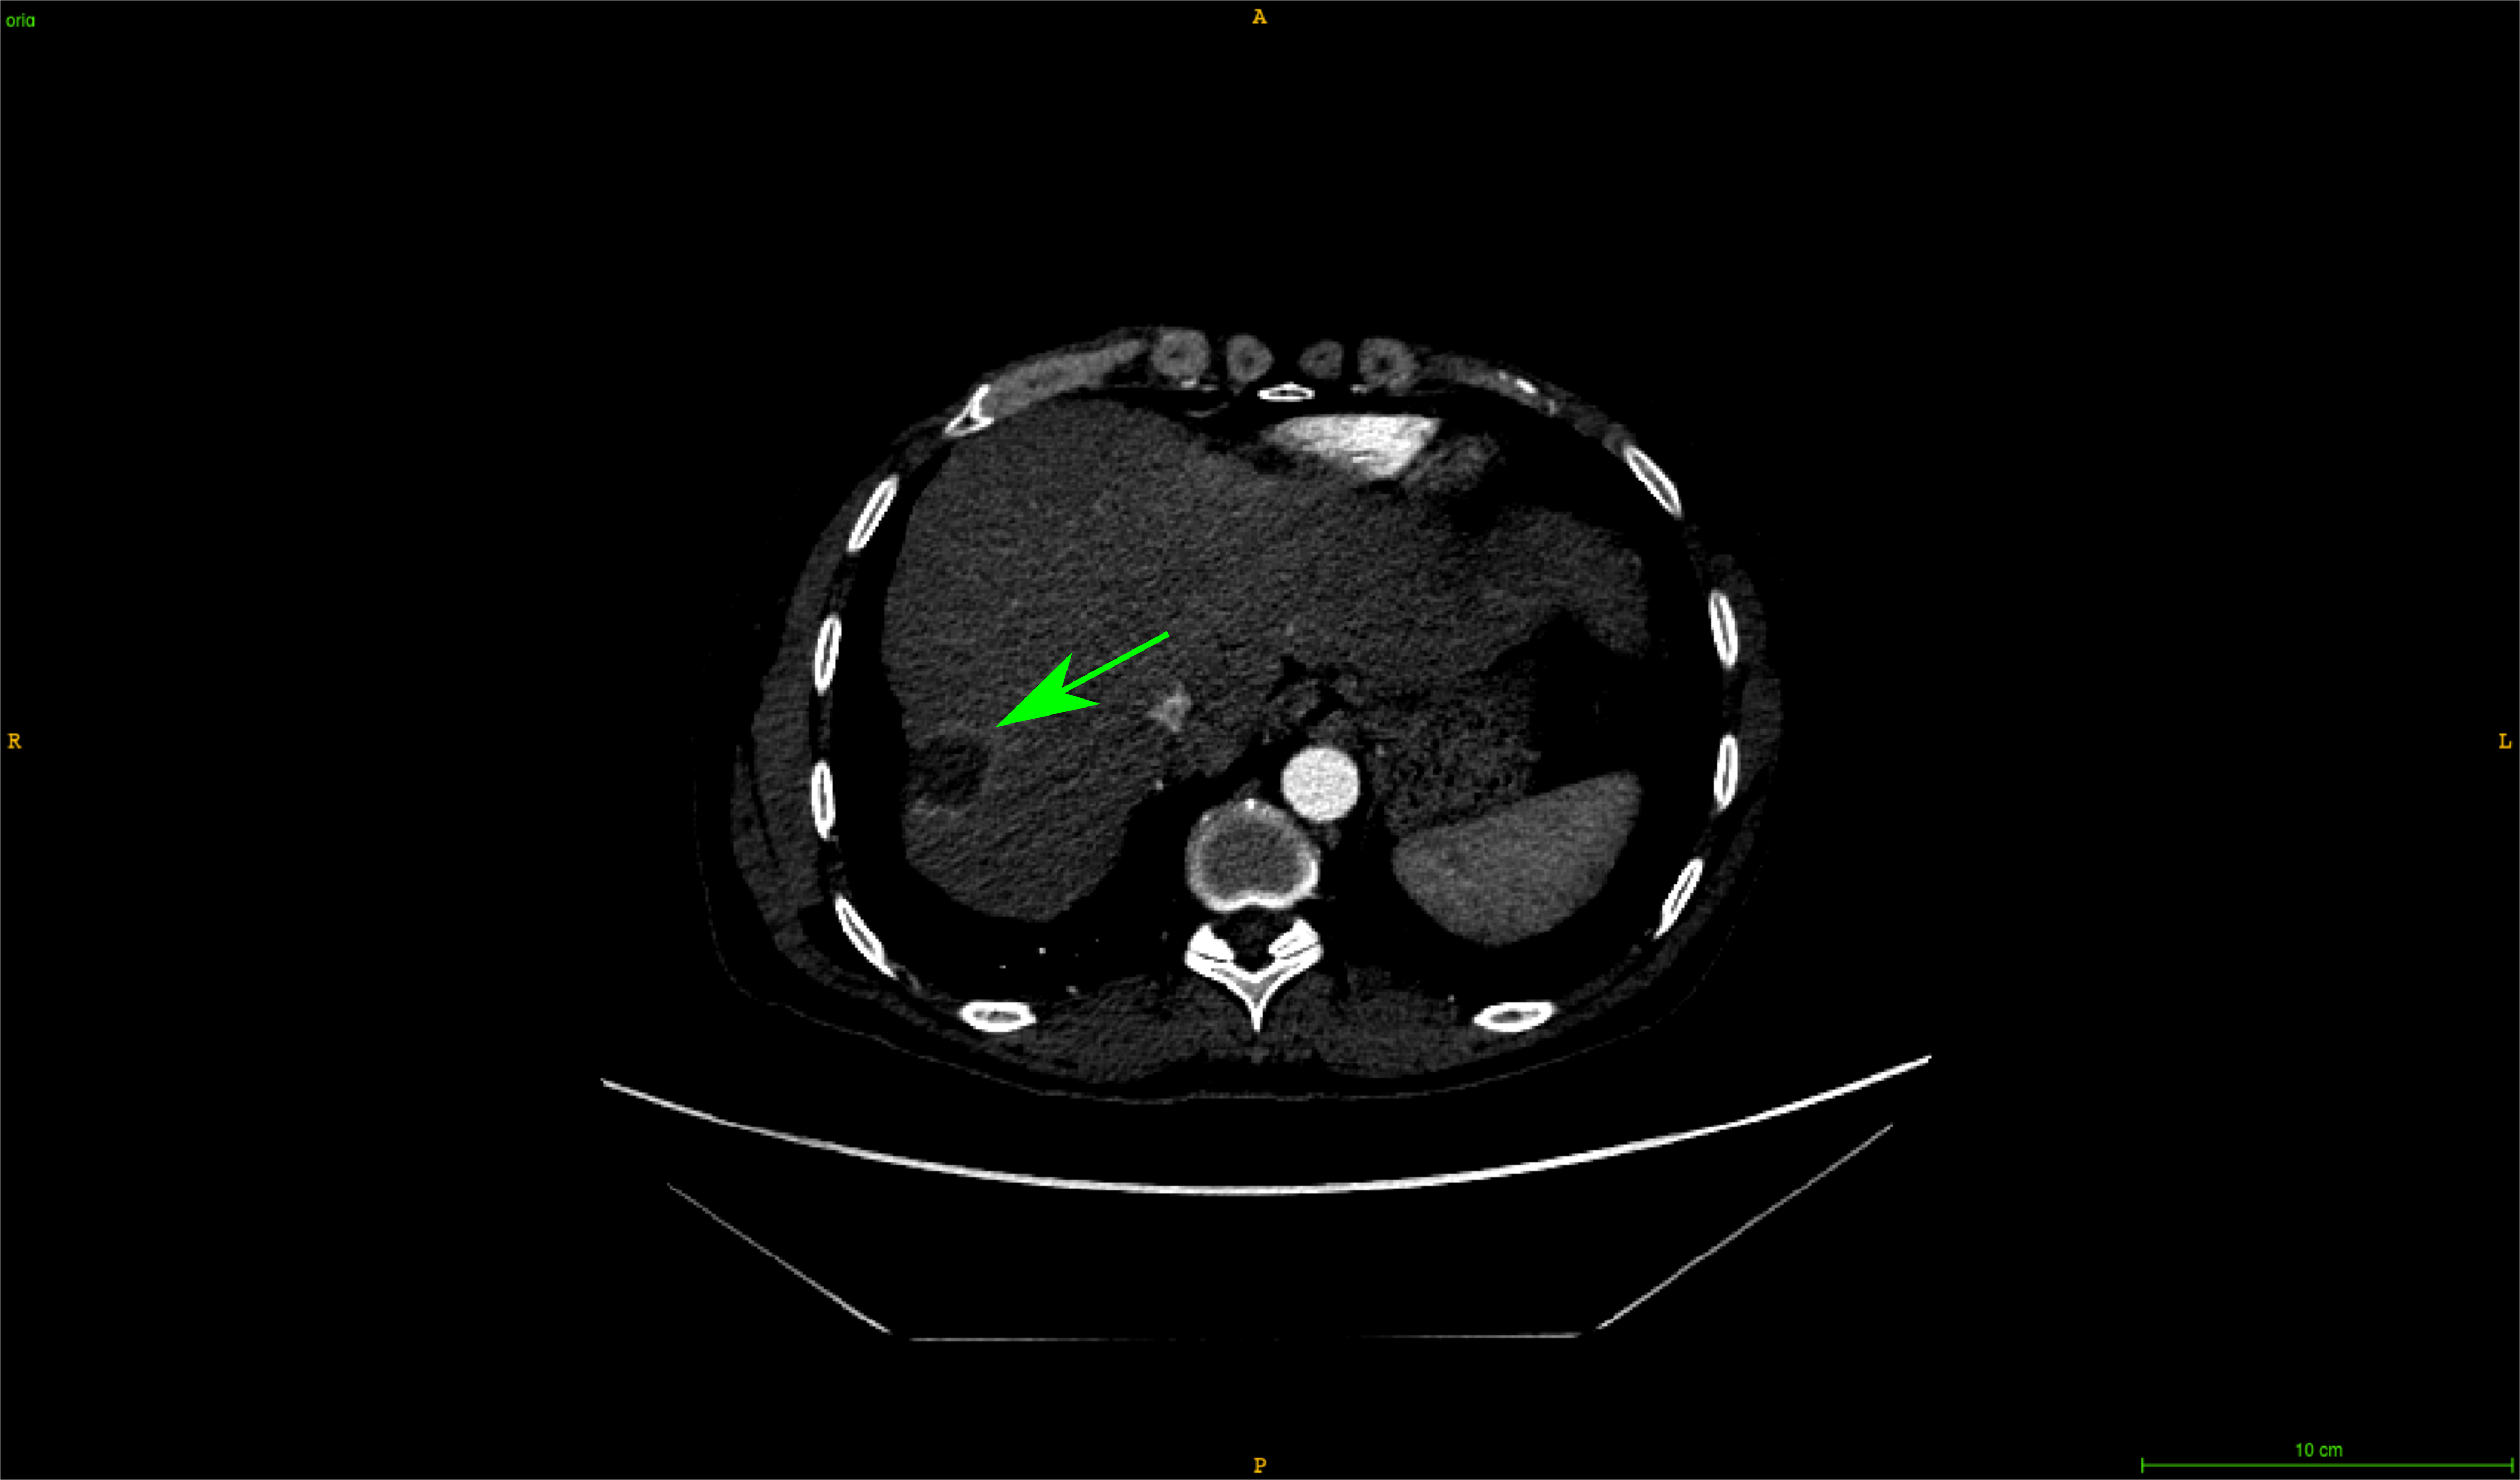
\includegraphics[width=\linewidth]{../Contributions/images/ImagingTraits/ResizeGDB_peritumoralEnhancement}
	\end{minipage} \hspace{-0.1cm}
	\begin{minipage}{0.45\linewidth}
		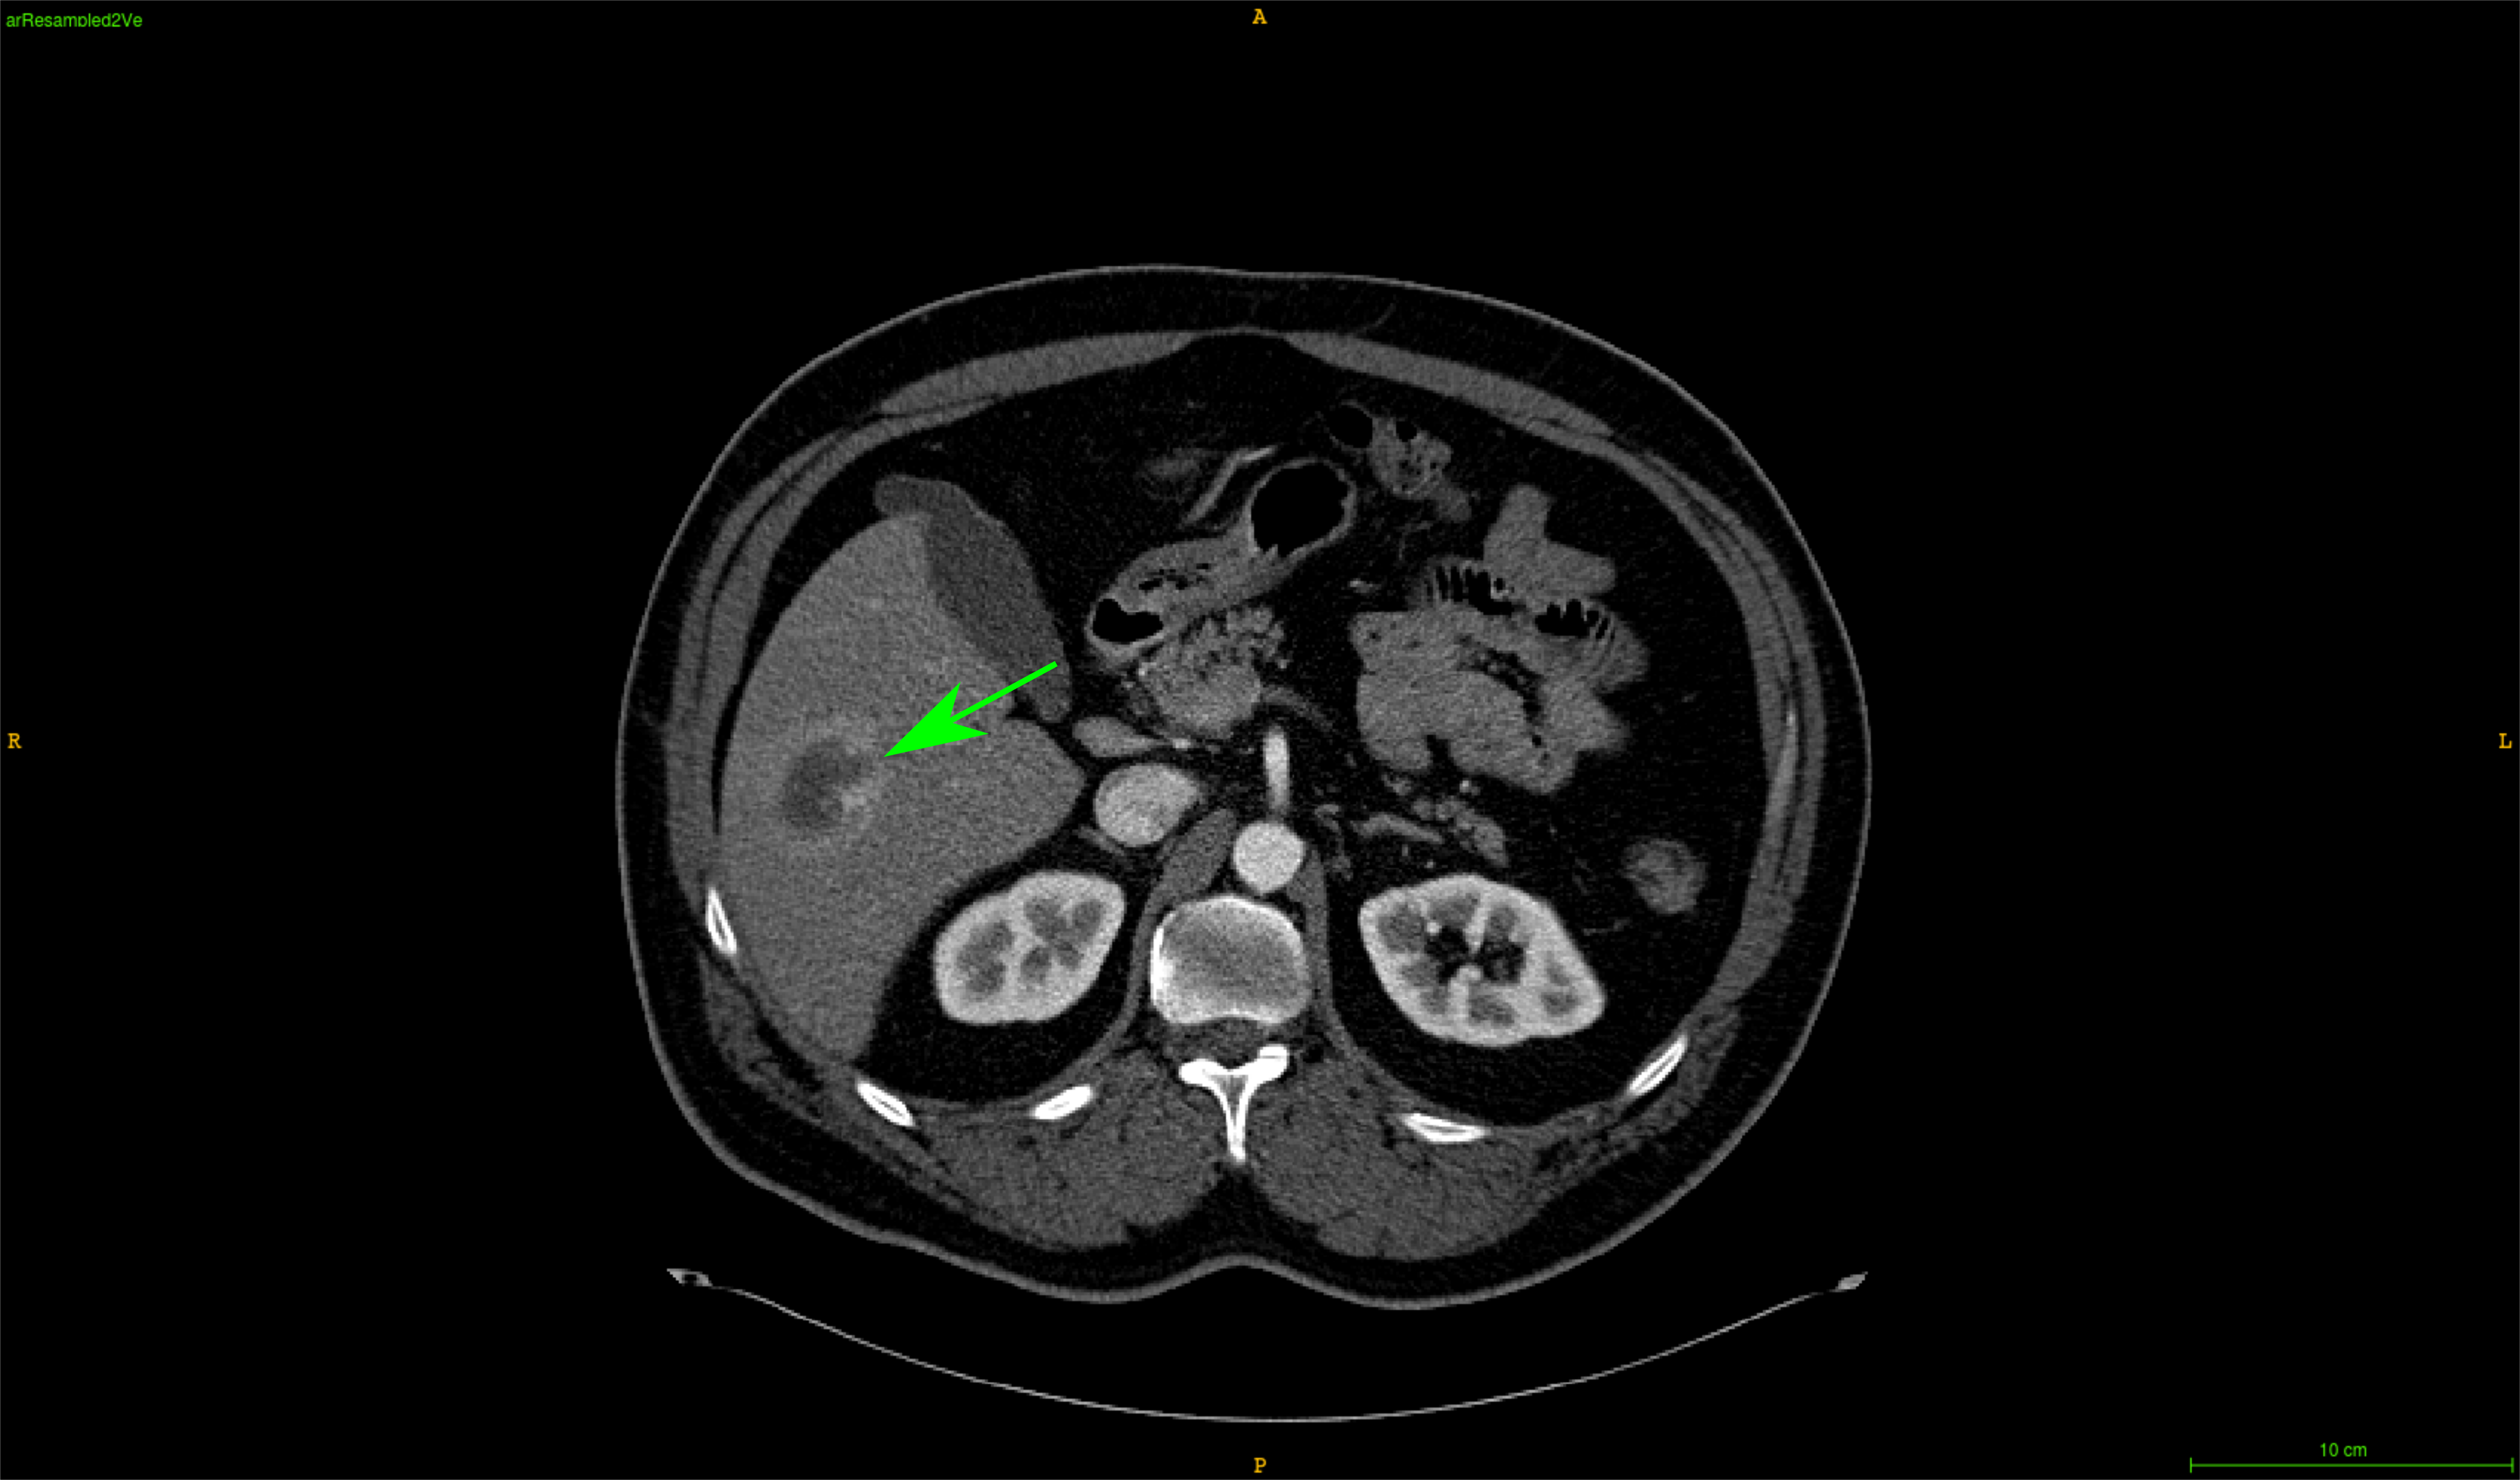
\includegraphics[width=\linewidth]{../Contributions/images/ImagingTraits/ResizeTCIA_peritumoralEnhancement}
	\end{minipage} \\
	\begin{minipage}{0.45\linewidth}
		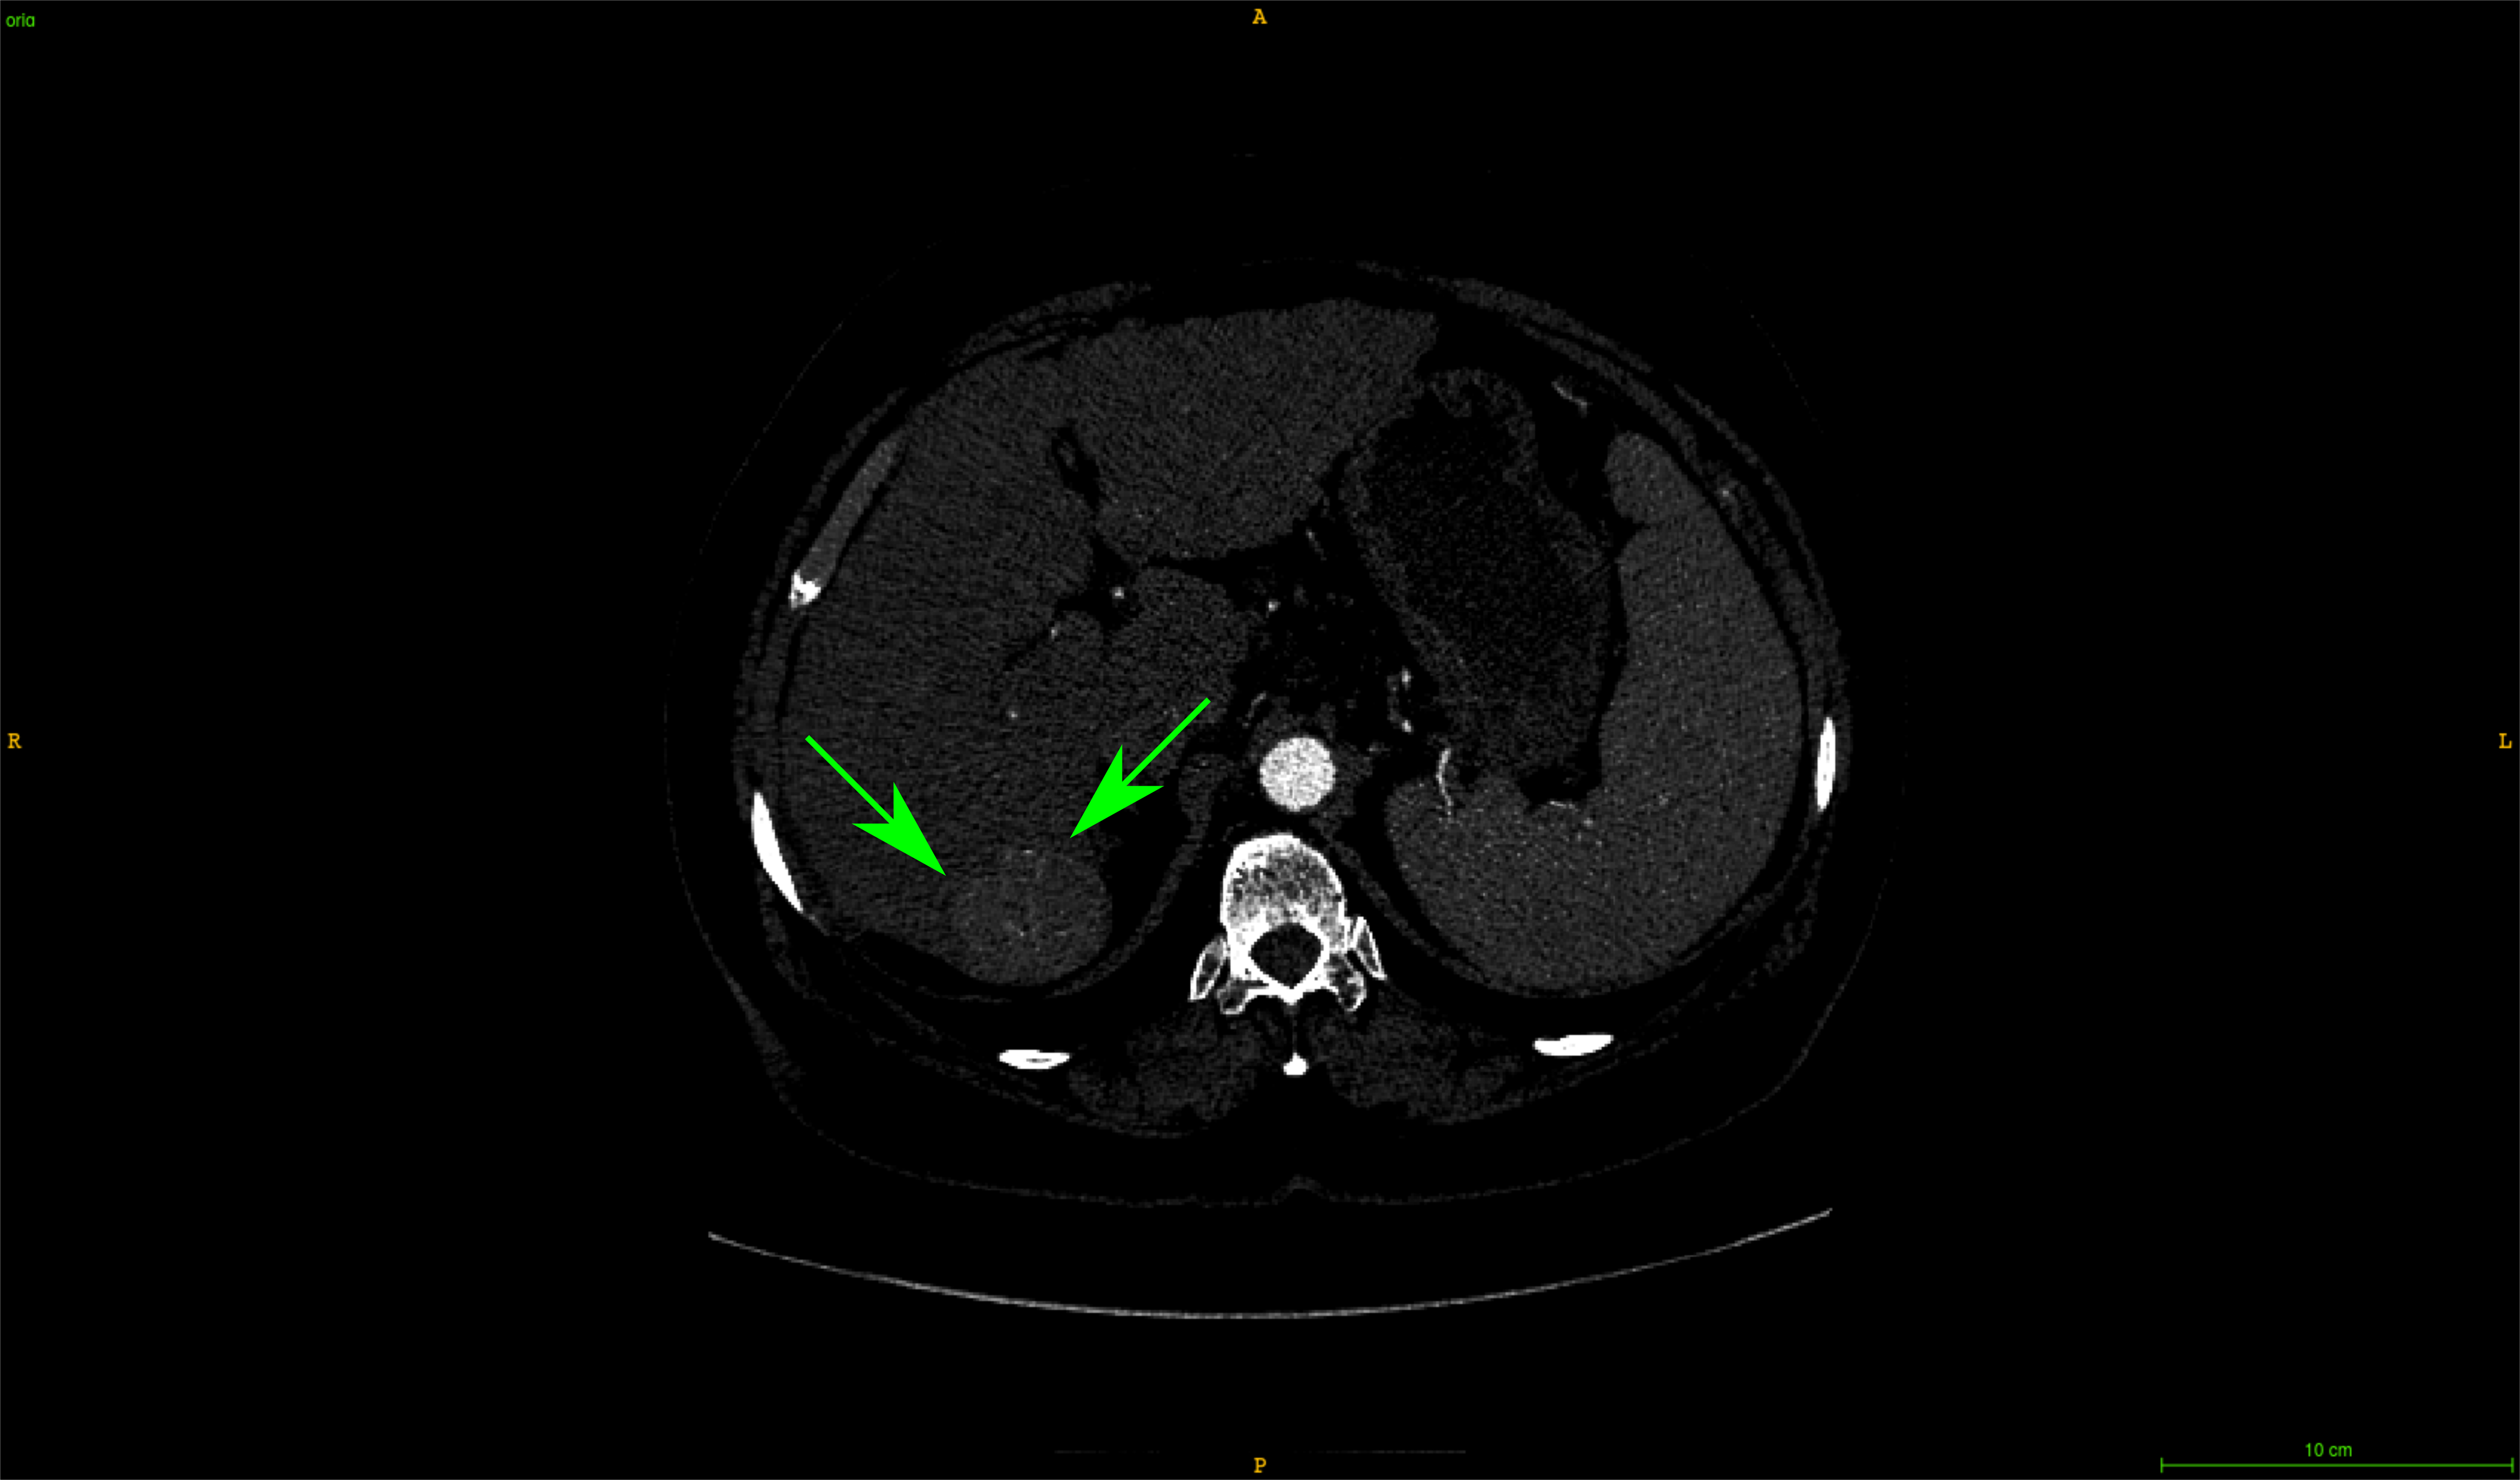
\includegraphics[width=\linewidth]{../Contributions/images/ImagingTraits/ResizeGDB_smoothMargins}
	\end{minipage} \hspace{-0.1cm}
	\begin{minipage}{0.45\linewidth}
		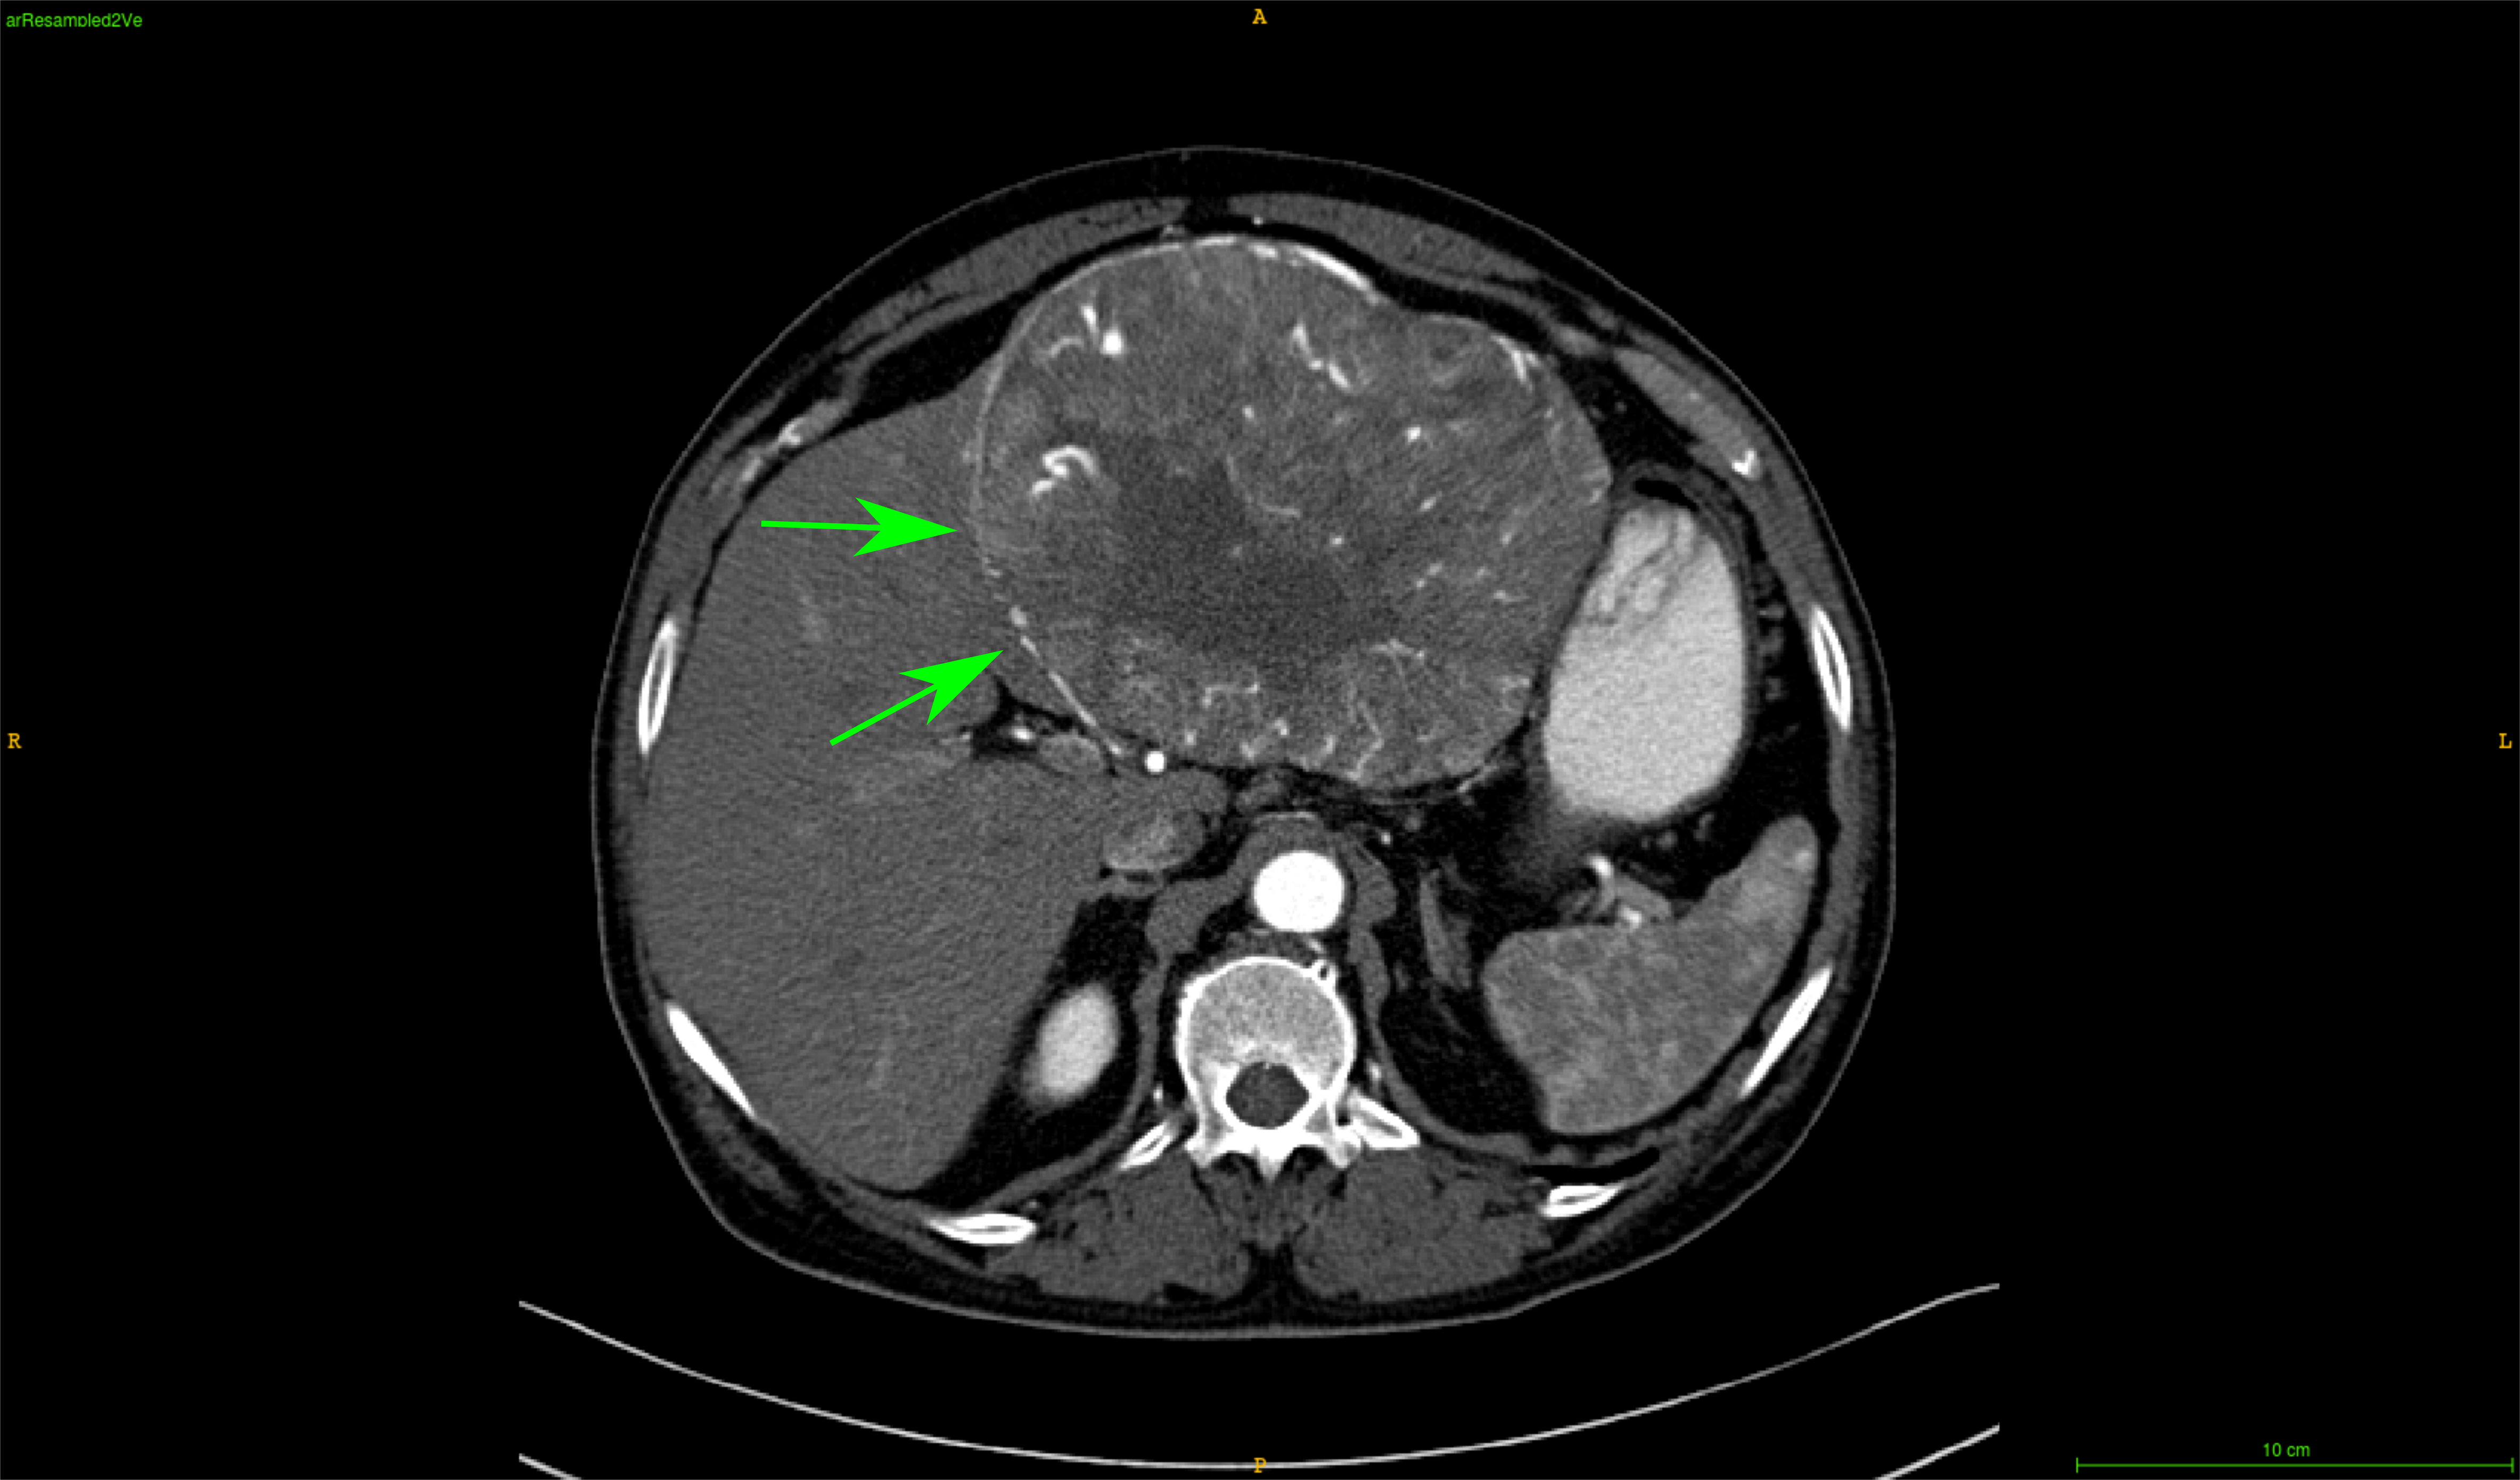
\includegraphics[width=\linewidth]{../Contributions/images/ImagingTraits/ResizeTCIA_smoothMargins}
	\end{minipage} \\
	\begin{minipage}{0.45\linewidth}
		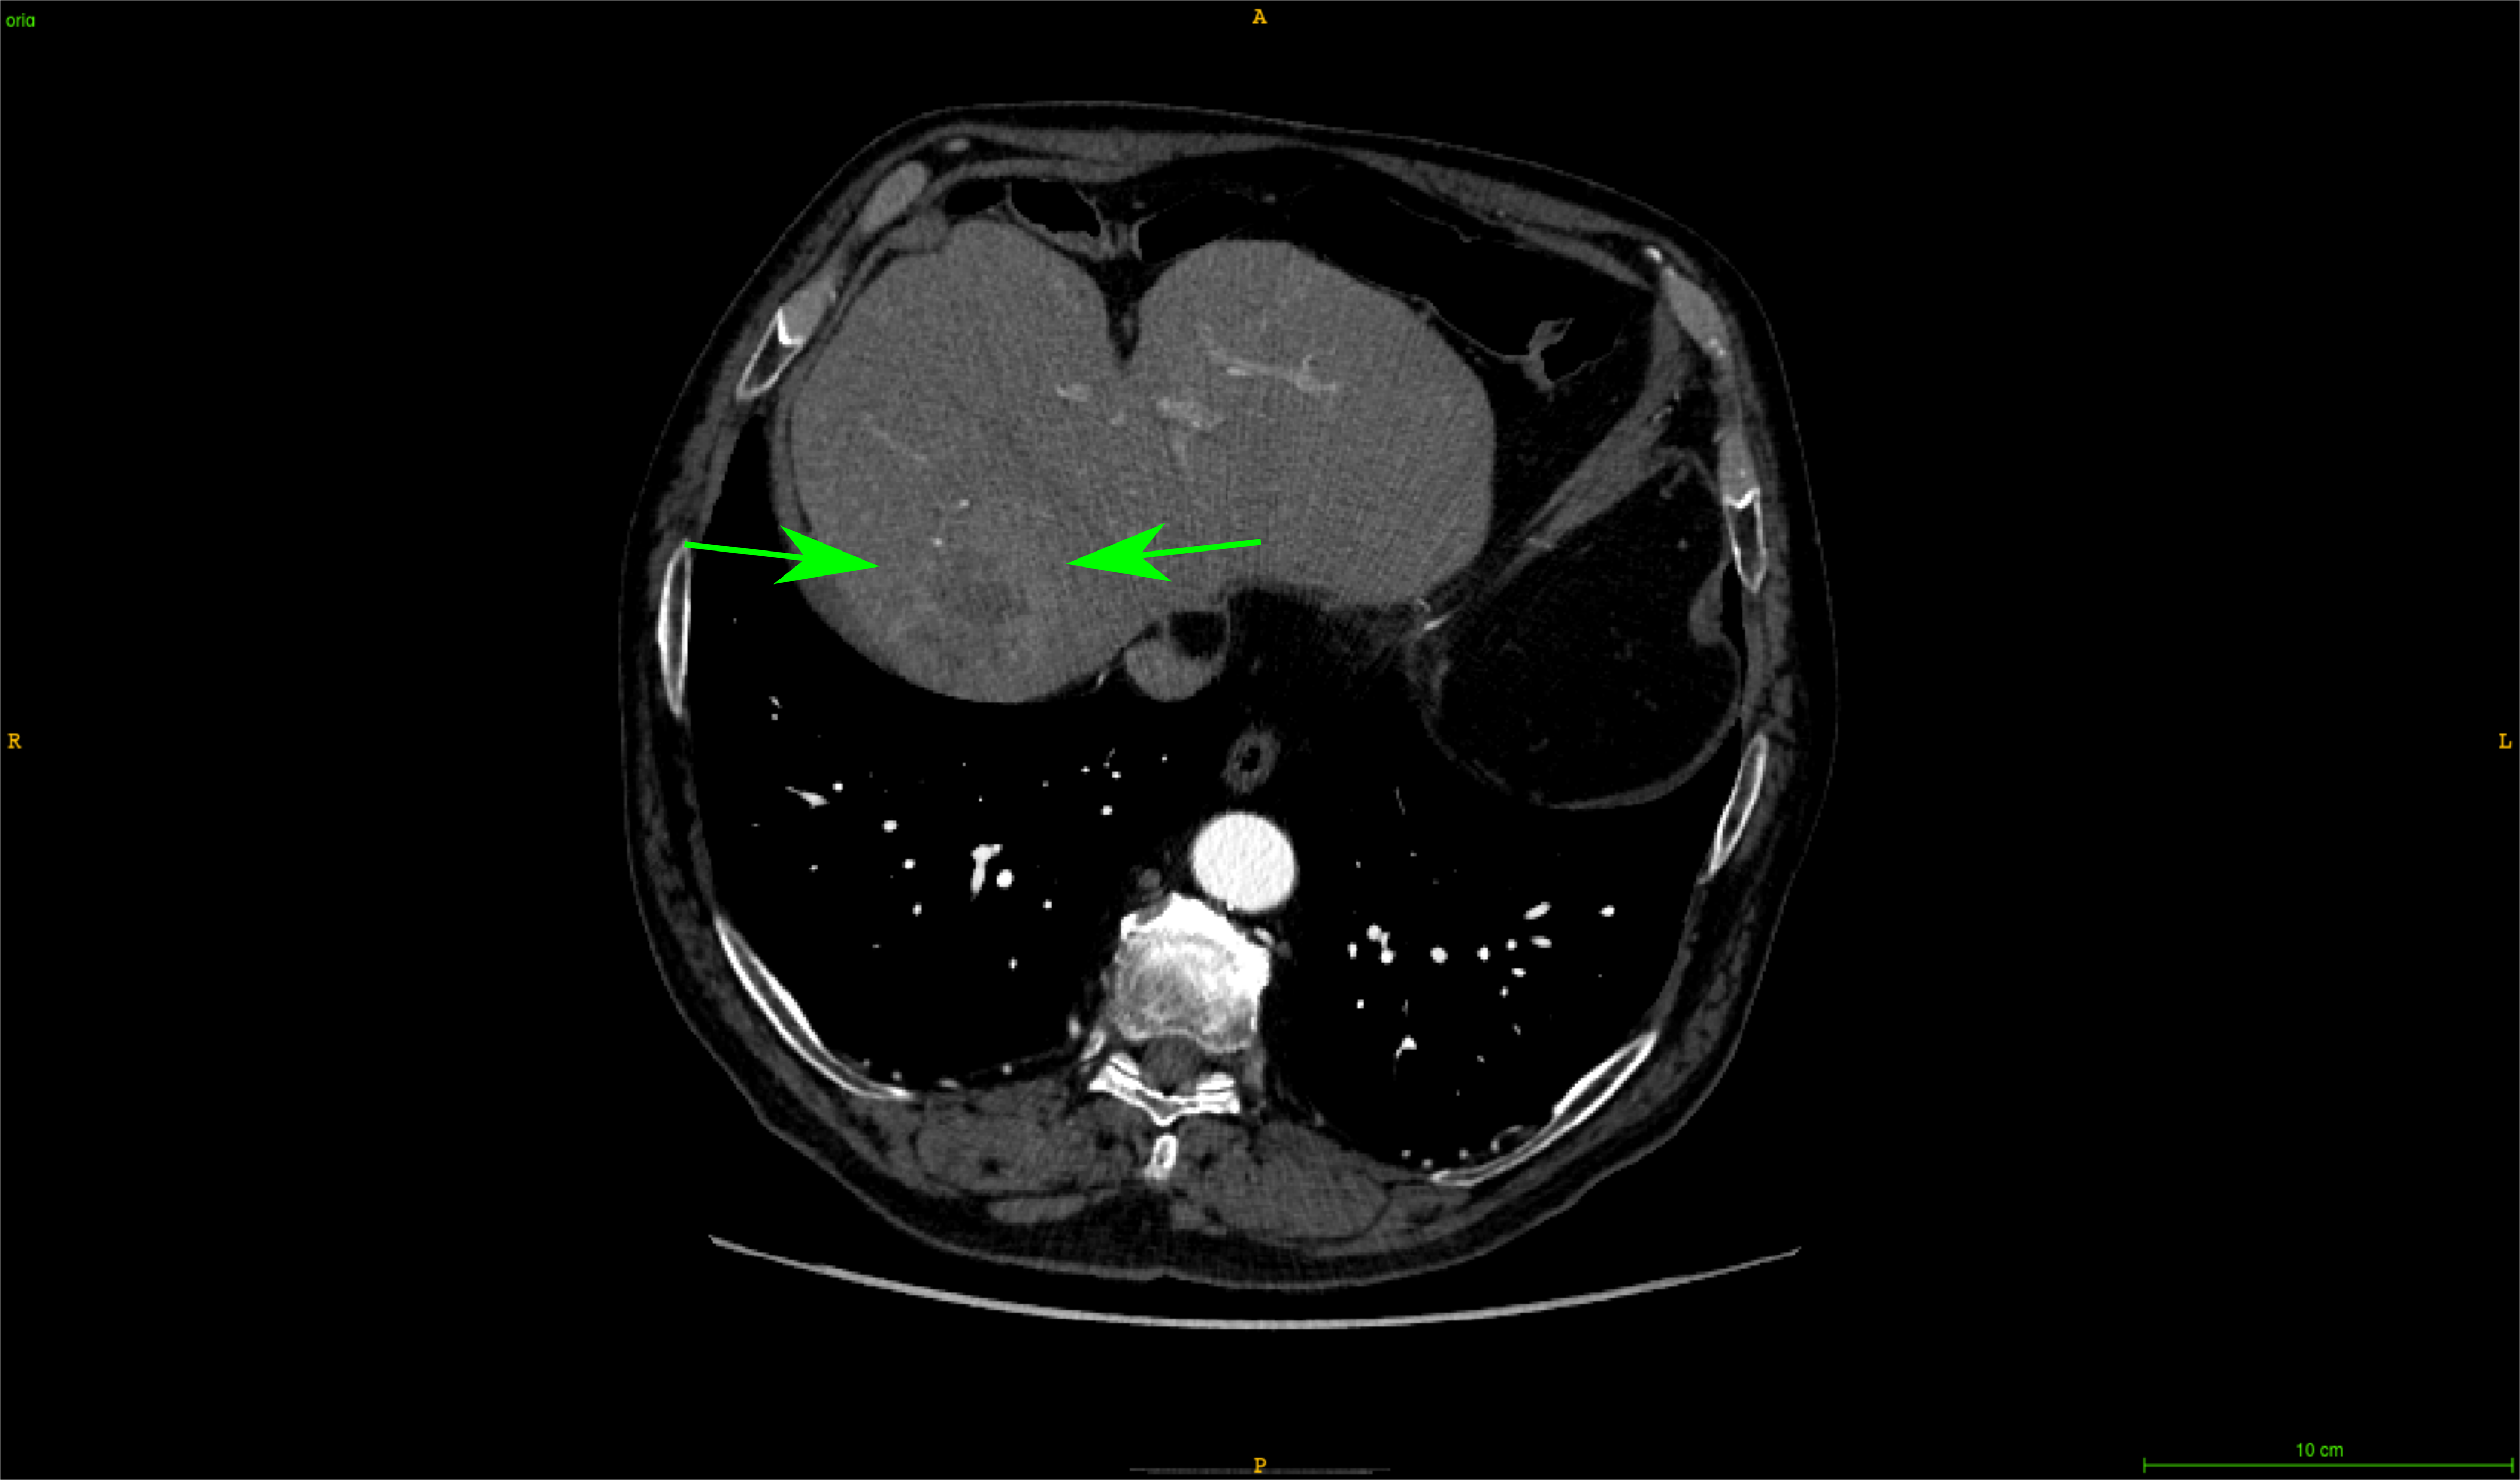
\includegraphics[width=\linewidth]{../Contributions/images/ImagingTraits/ResizeGDB_nonSmoothMargins}
	\end{minipage} \hspace{-0.1cm}
	\begin{minipage}{0.45\linewidth}
		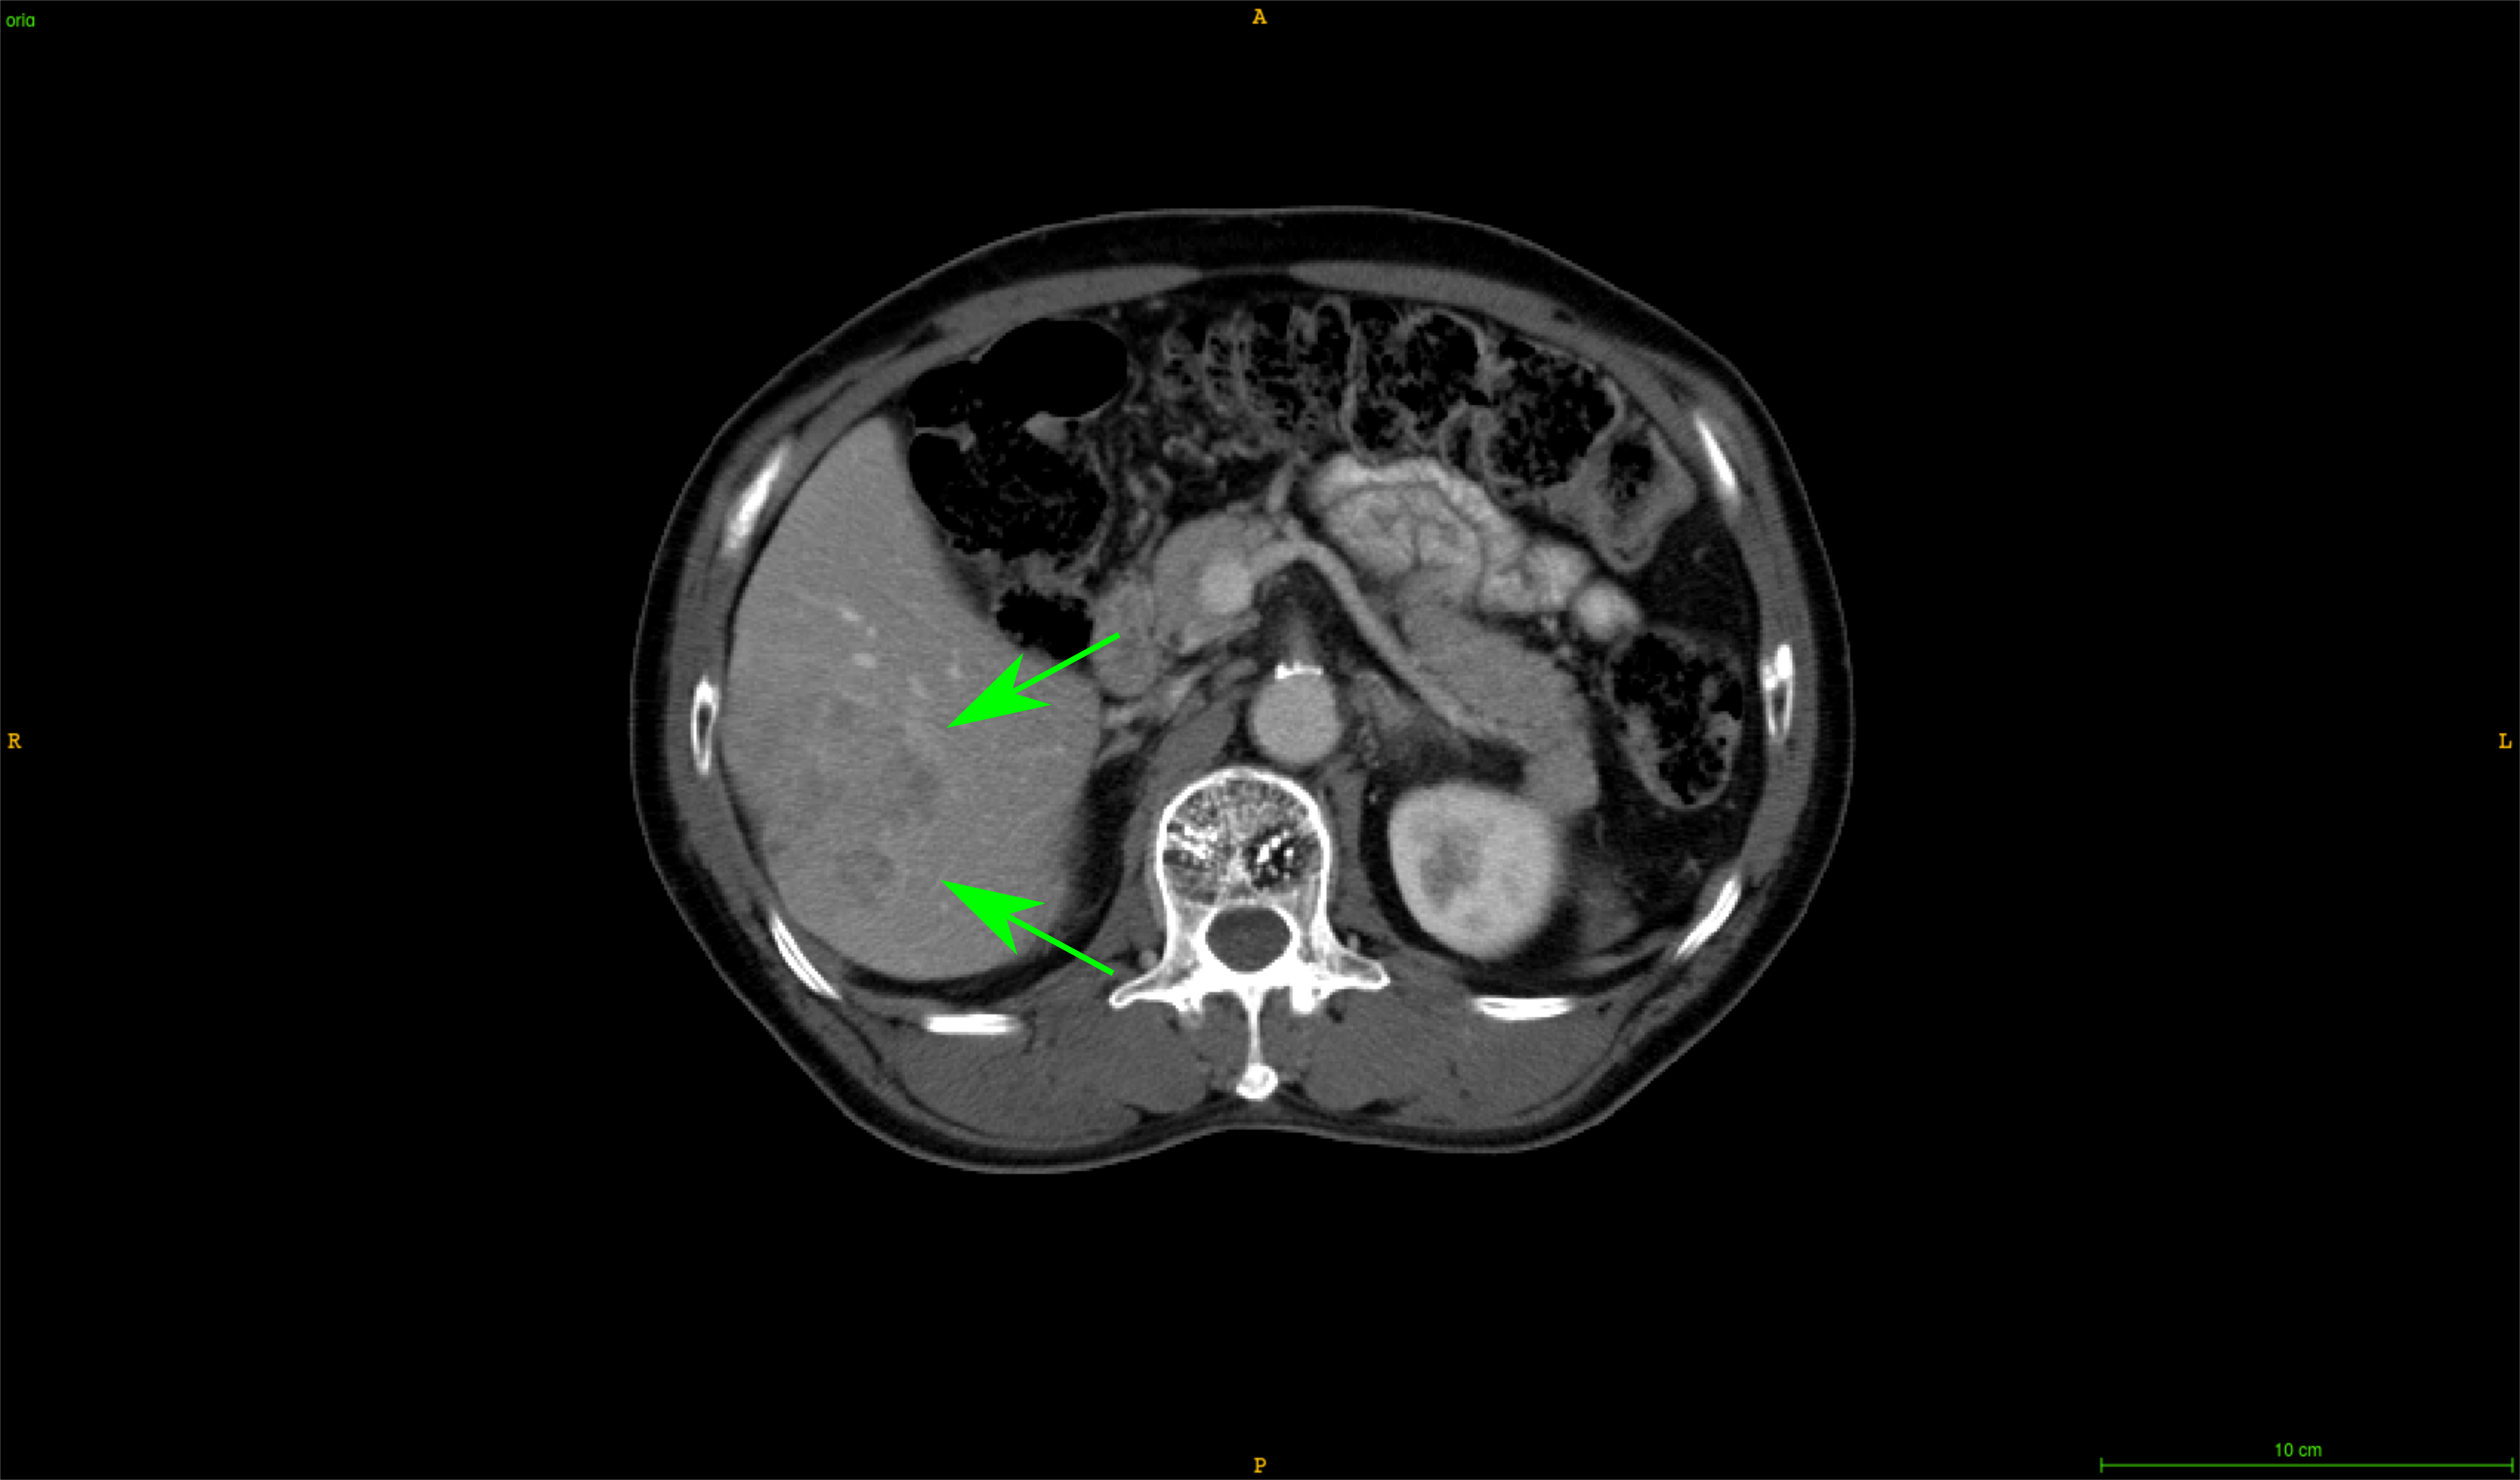
\includegraphics[width=\linewidth]{../Contributions/images/ImagingTraits/ResizeTCIA_nonSmoothMargins}
	\end{minipage} \\
	\begin{minipage}{0.45\linewidth}
		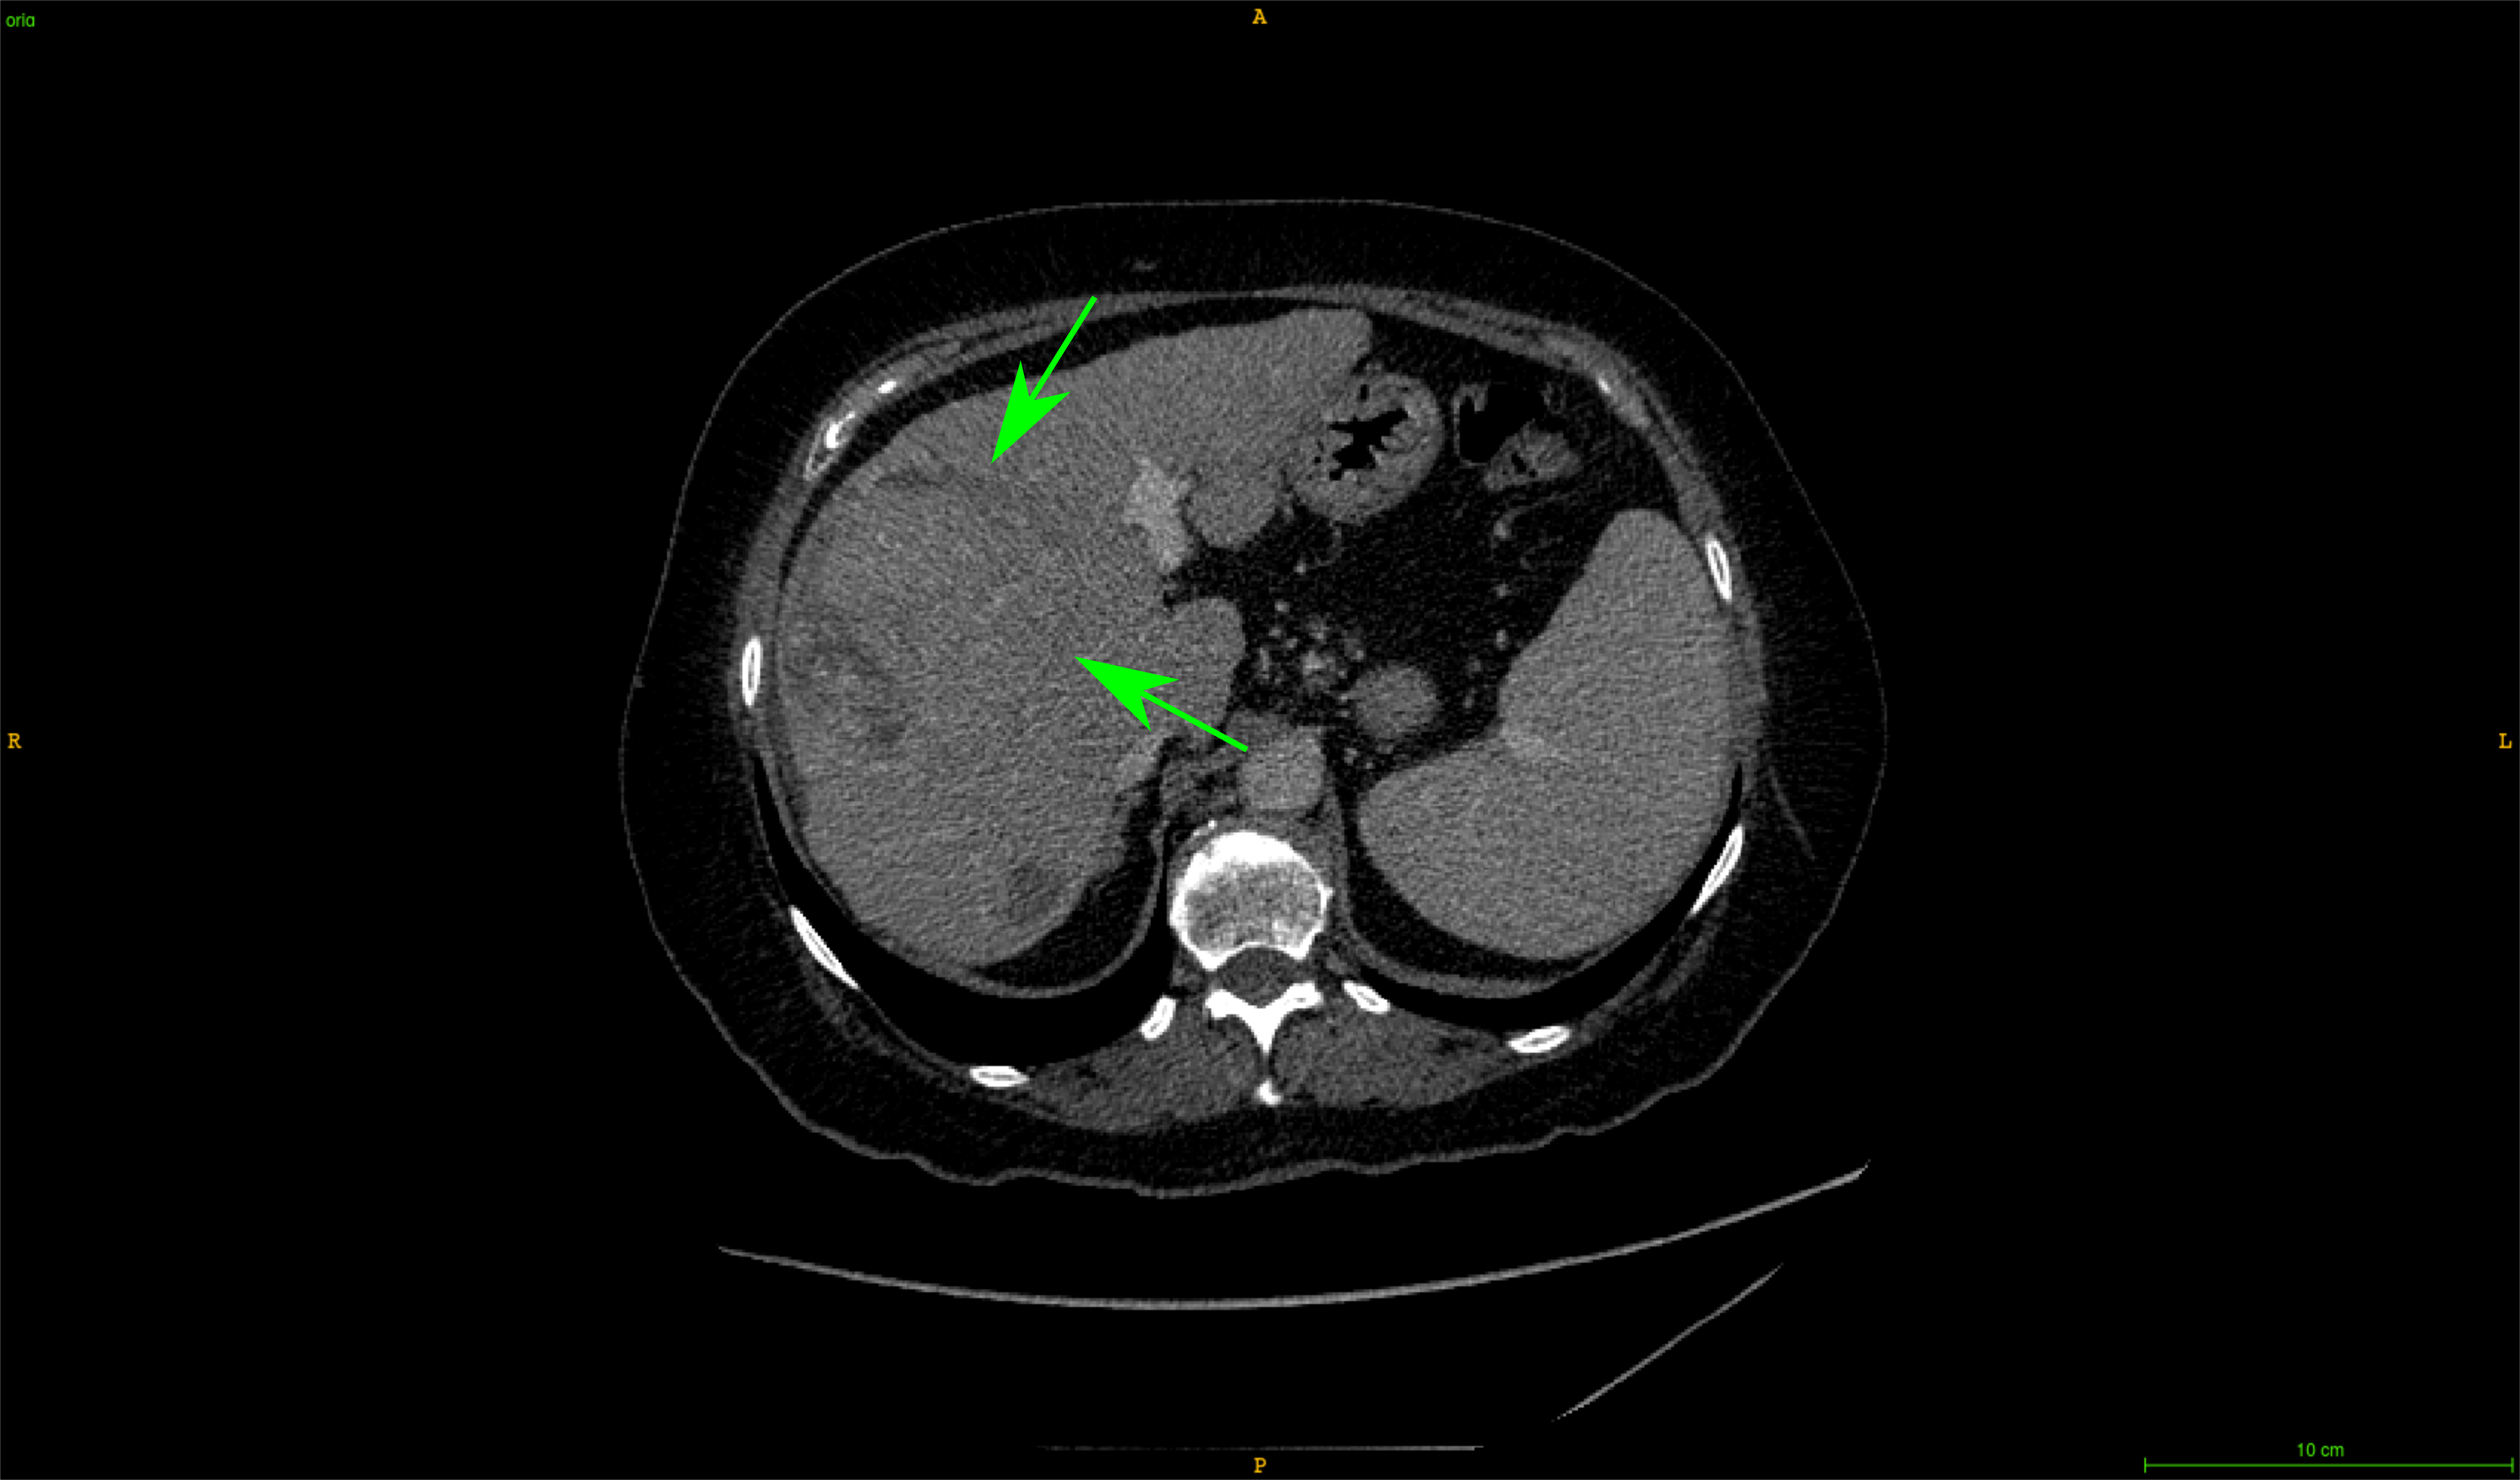
\includegraphics[width=\linewidth]{../Contributions/images/ImagingTraits/ResizeGDB_halo}
	\end{minipage} \hspace{-0.1cm}
	\begin{minipage}{0.45\linewidth}
		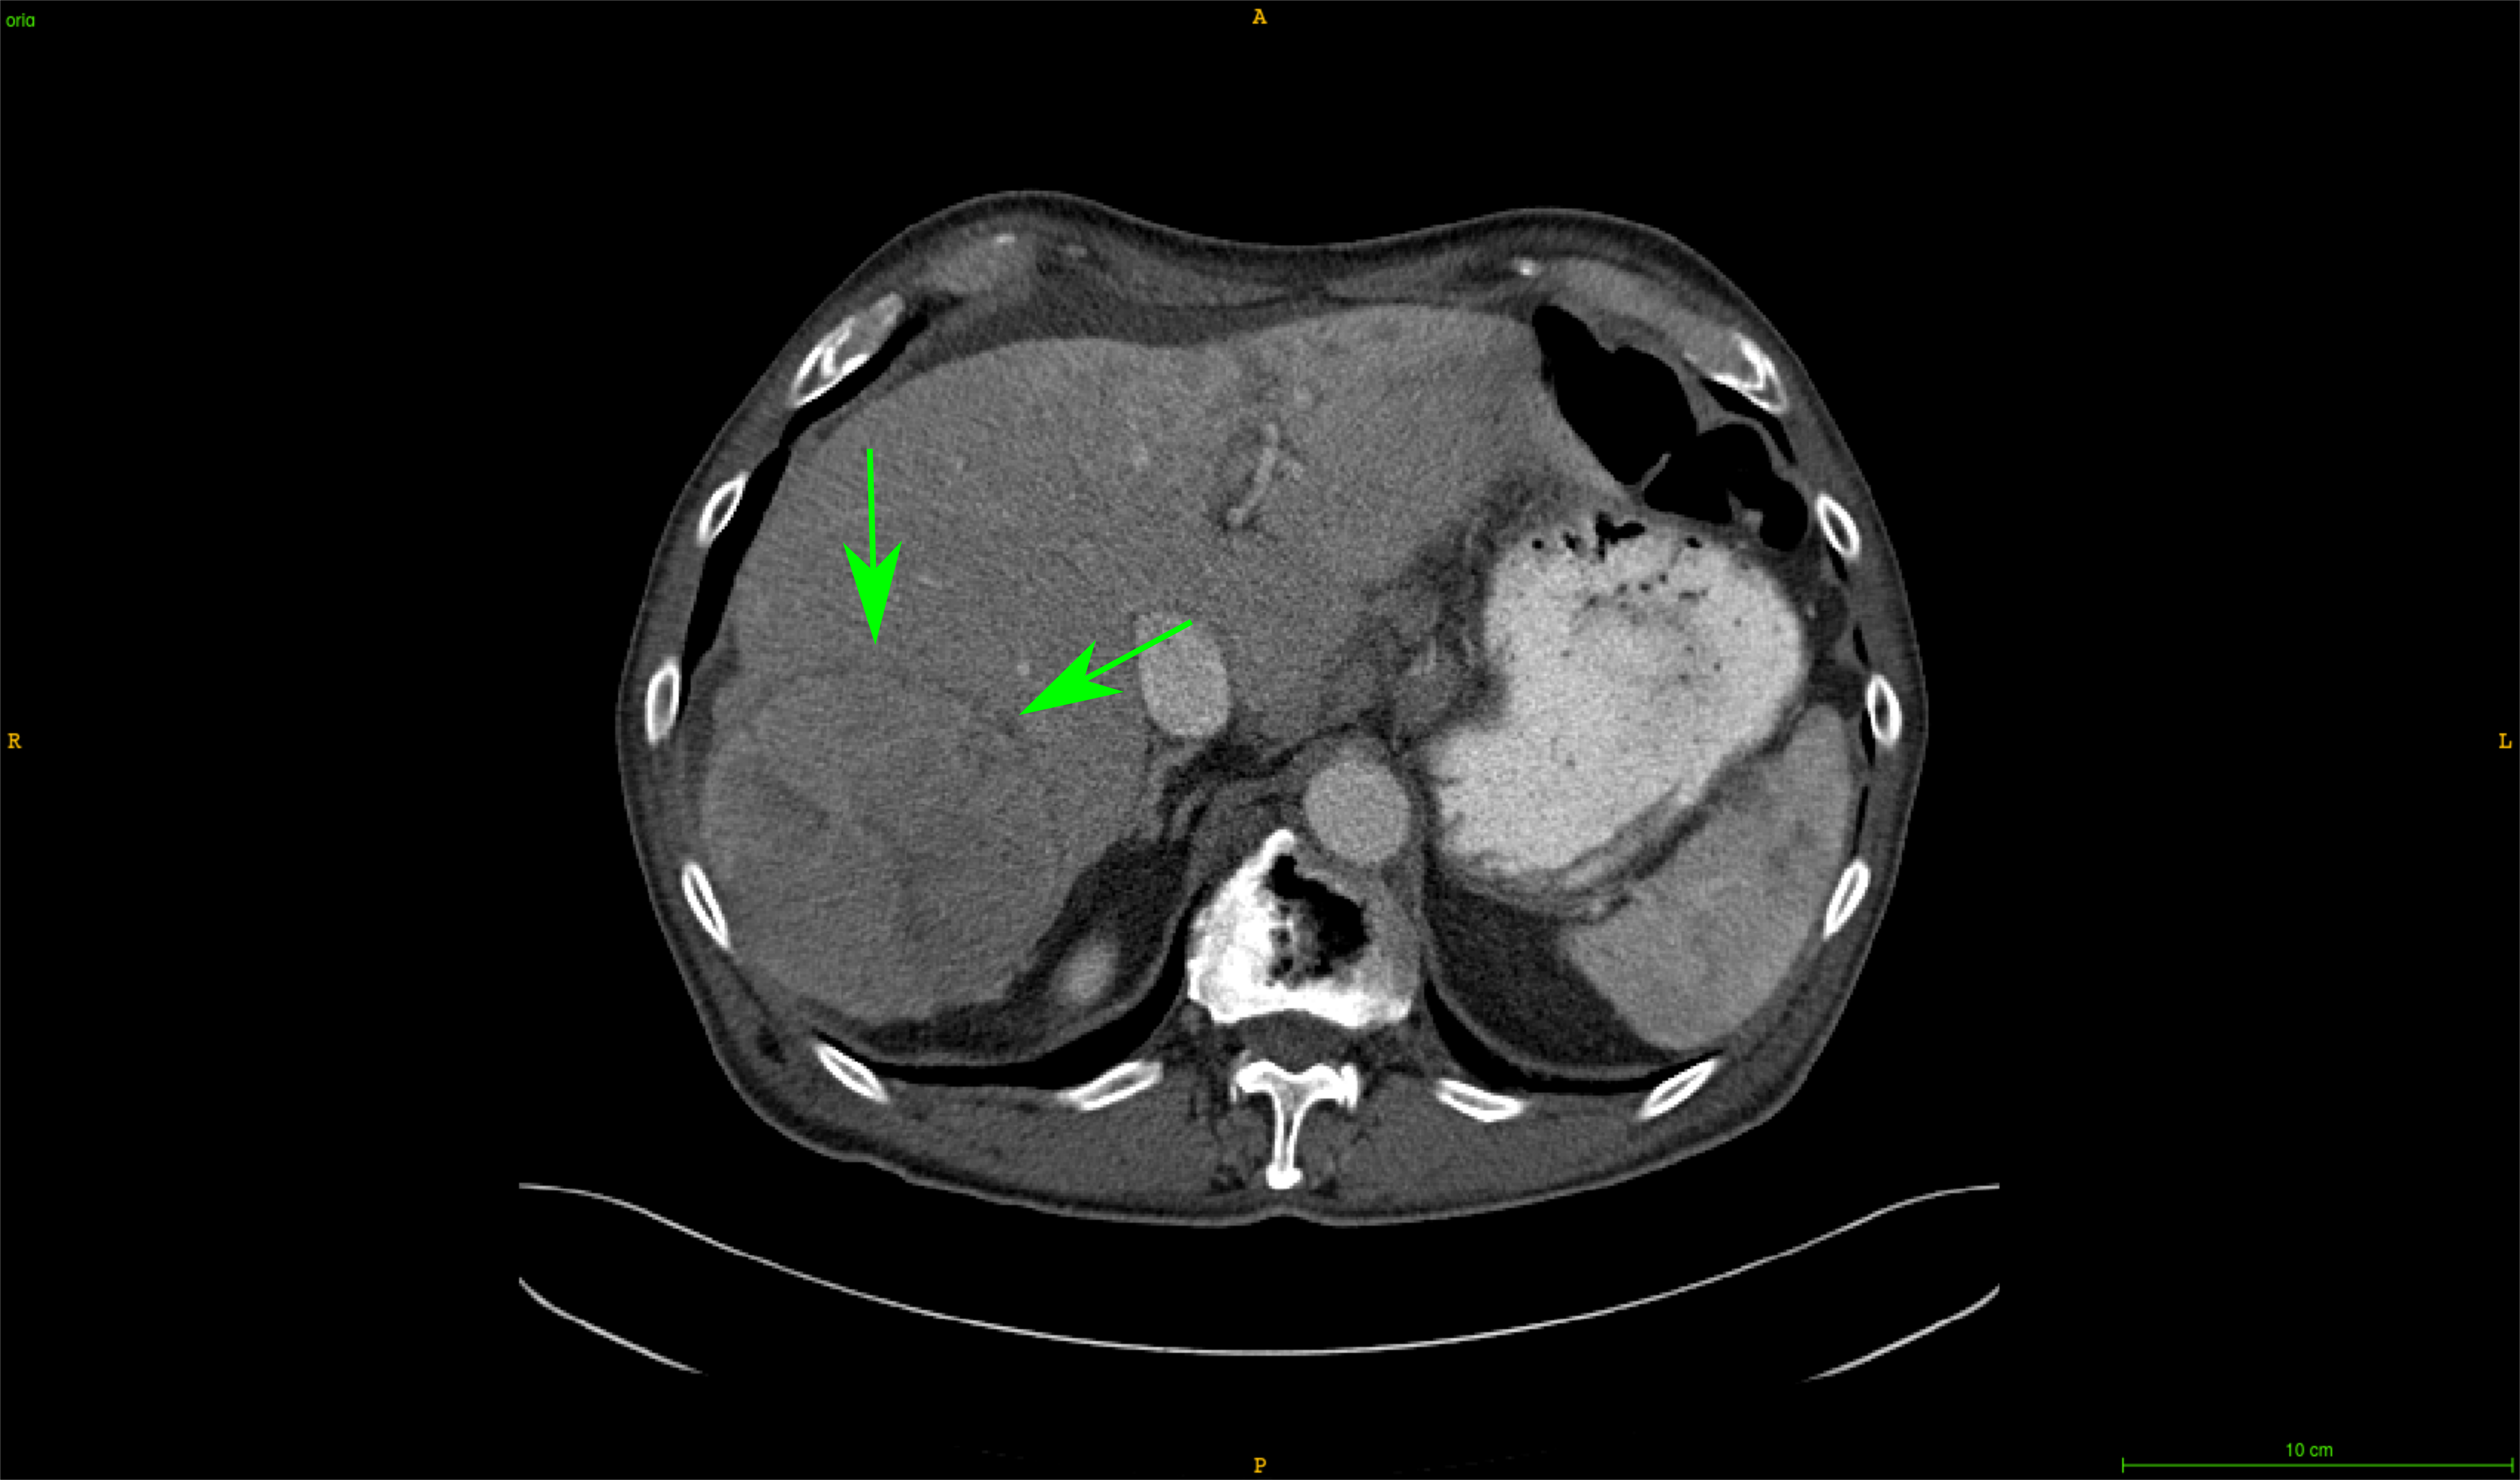
\includegraphics[width=\linewidth]{../Contributions/images/ImagingTraits/ResizeTCIA_halo}
	\end{minipage}
	\caption{Examples of tumor characteristic imaging traits relative to the tumor border present in both training and test datasets. Left: \textbf{\lmttfont{G-dB}} images, right: \textbf{\lmttfont{TCIA-dB}} images. First row: peritumoral enhancement, which can be defined by the presence of a detectable region of enhancement adjacent to the tumor border in the arterial phase. Second and third rows: illustration of the tumor margin, that can be categorized as a smooth margin (second row) when facing nodular tumors with smooth contours or as non-smooth margin (third row) when facing non-nodular tumors with an irregular margin with budding portions at the periphery in both \ac{ar} and \ac{pv} images. Bottom row: hypoattenuating halo, defined as a rim of hypoattenuation partially or completely circumscribing the tumor on peritumoral \ac{pv} images. }
	\label{fig:InterDb_imagingTraits}
\end{figure}
\begin{figure}[!ht]
	\centering
	\begin{minipage}{0.45\linewidth}
		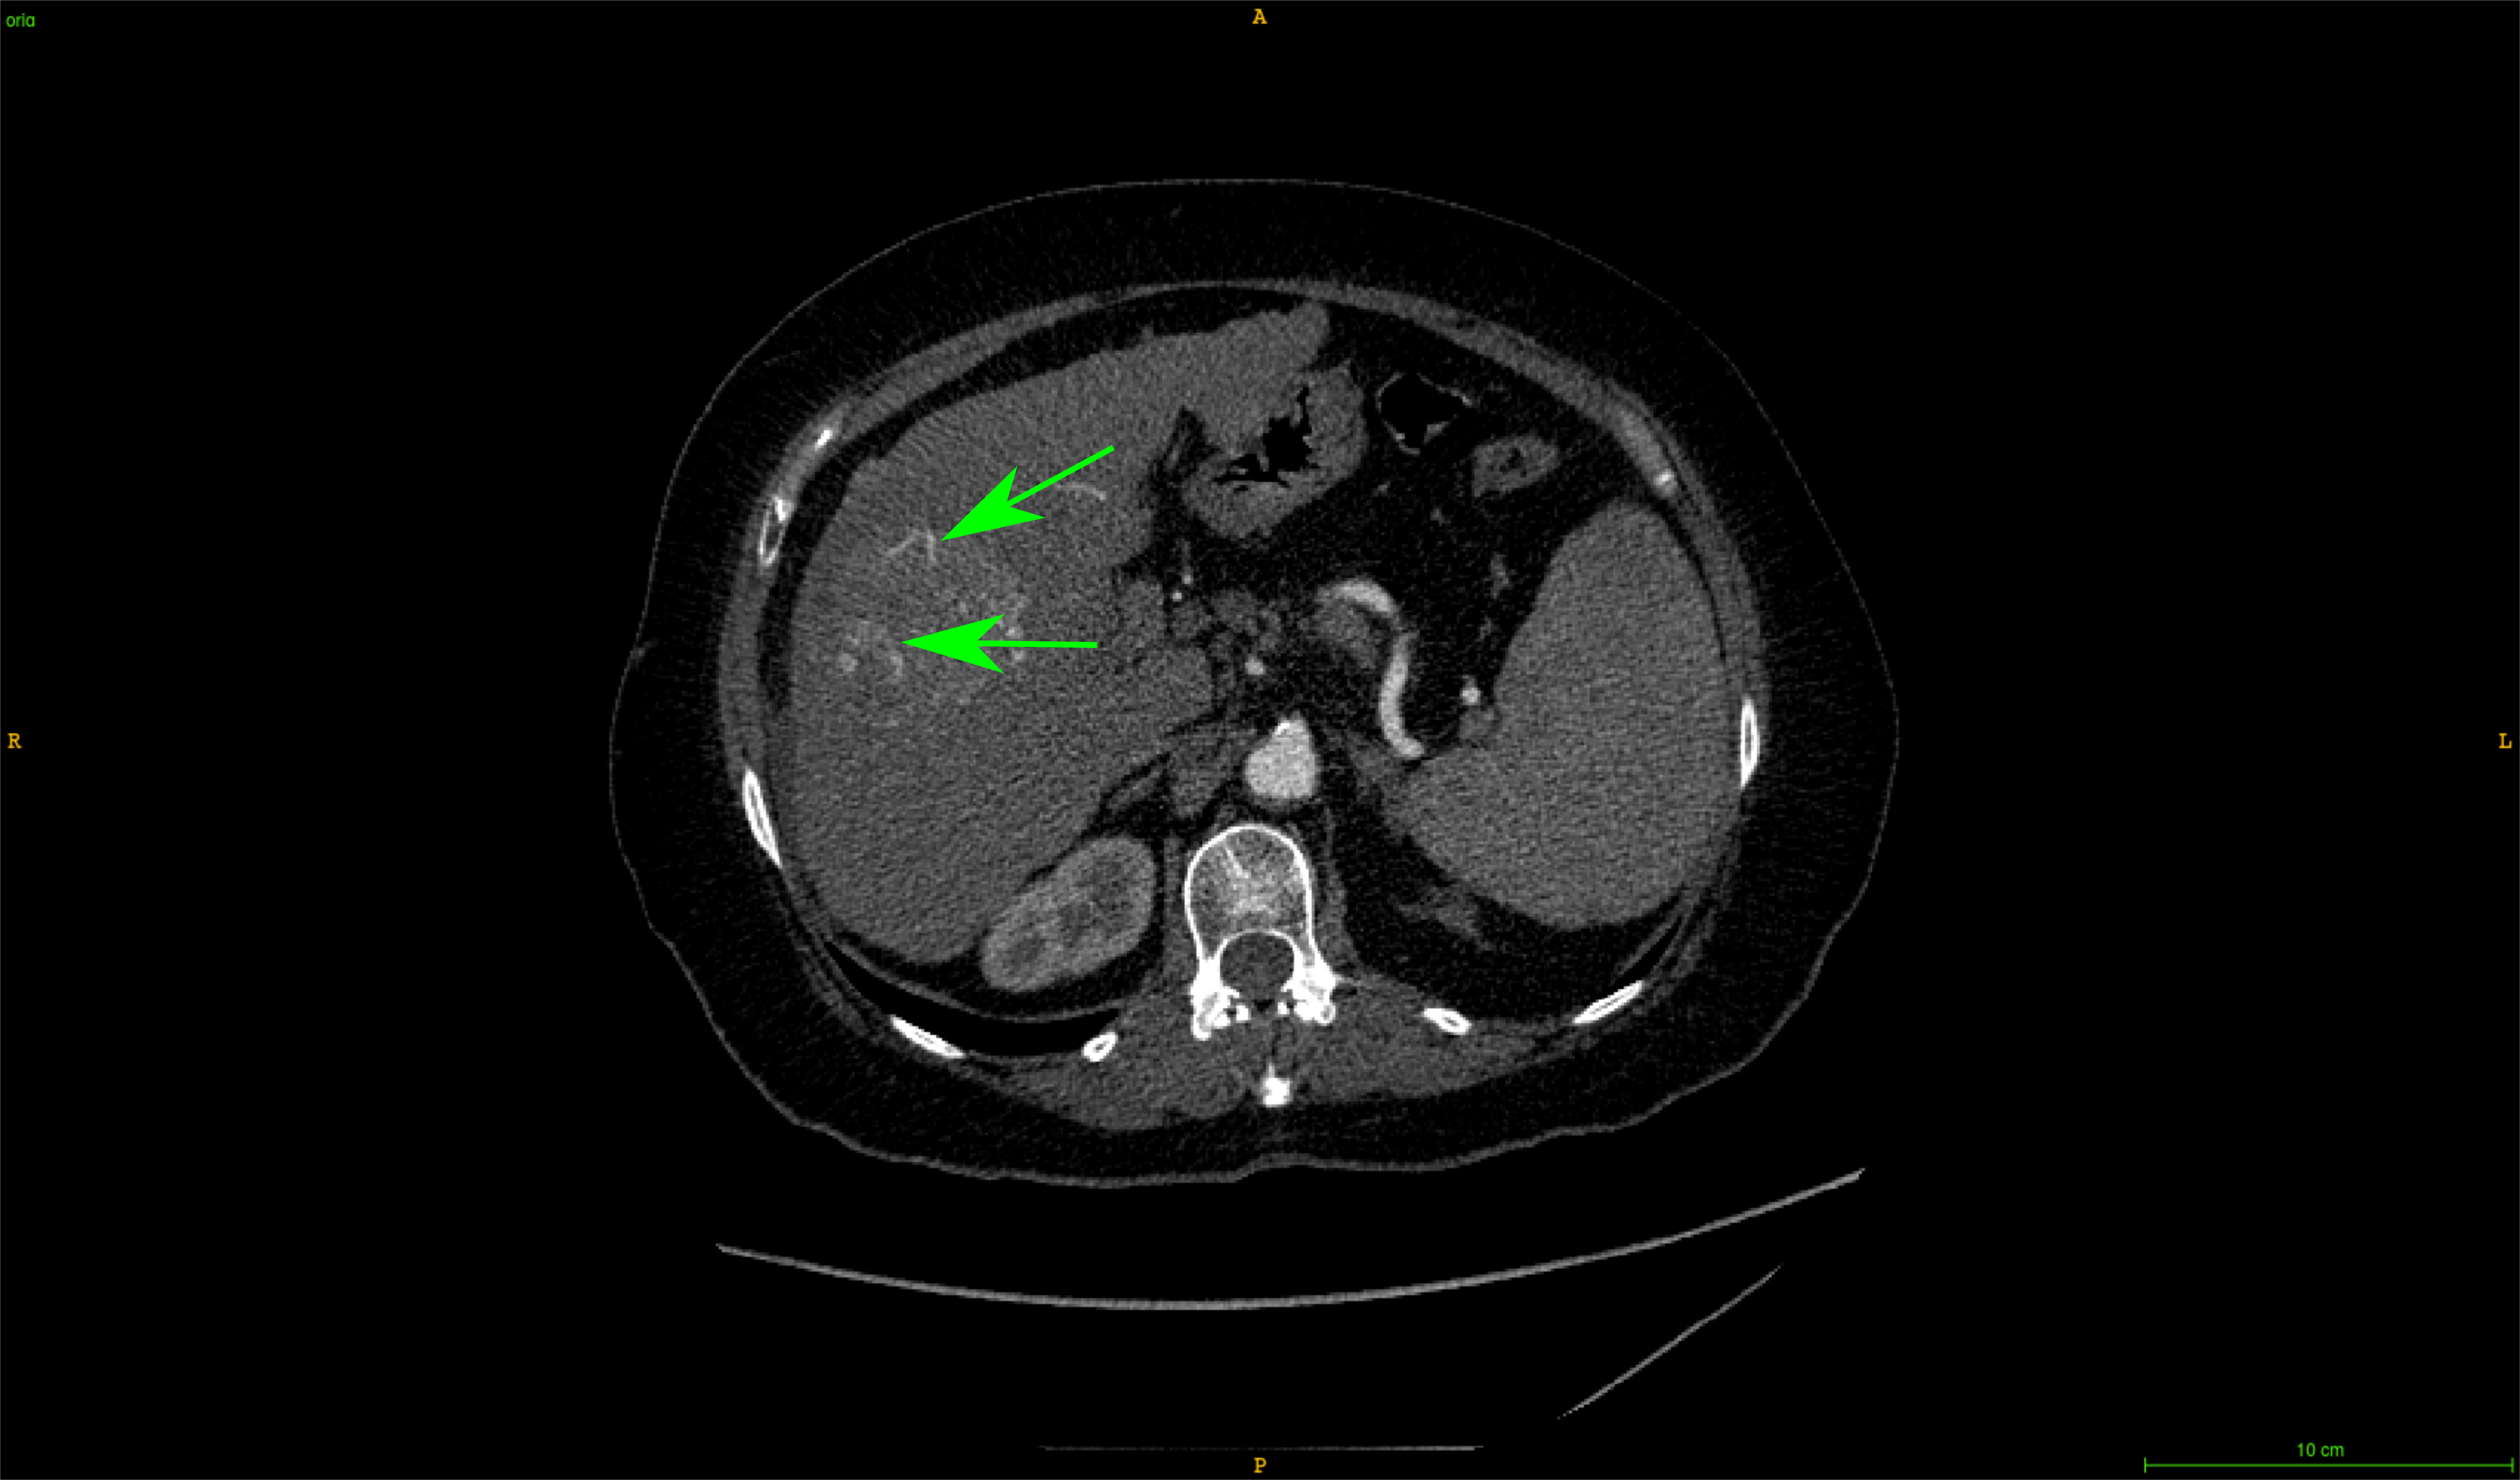
\includegraphics[width=\linewidth]{../Contributions/images/ImagingTraits/ResizeGDB_internalArteries}
	\end{minipage} \hspace{-0.1cm}
	\begin{minipage}{0.45\linewidth}
		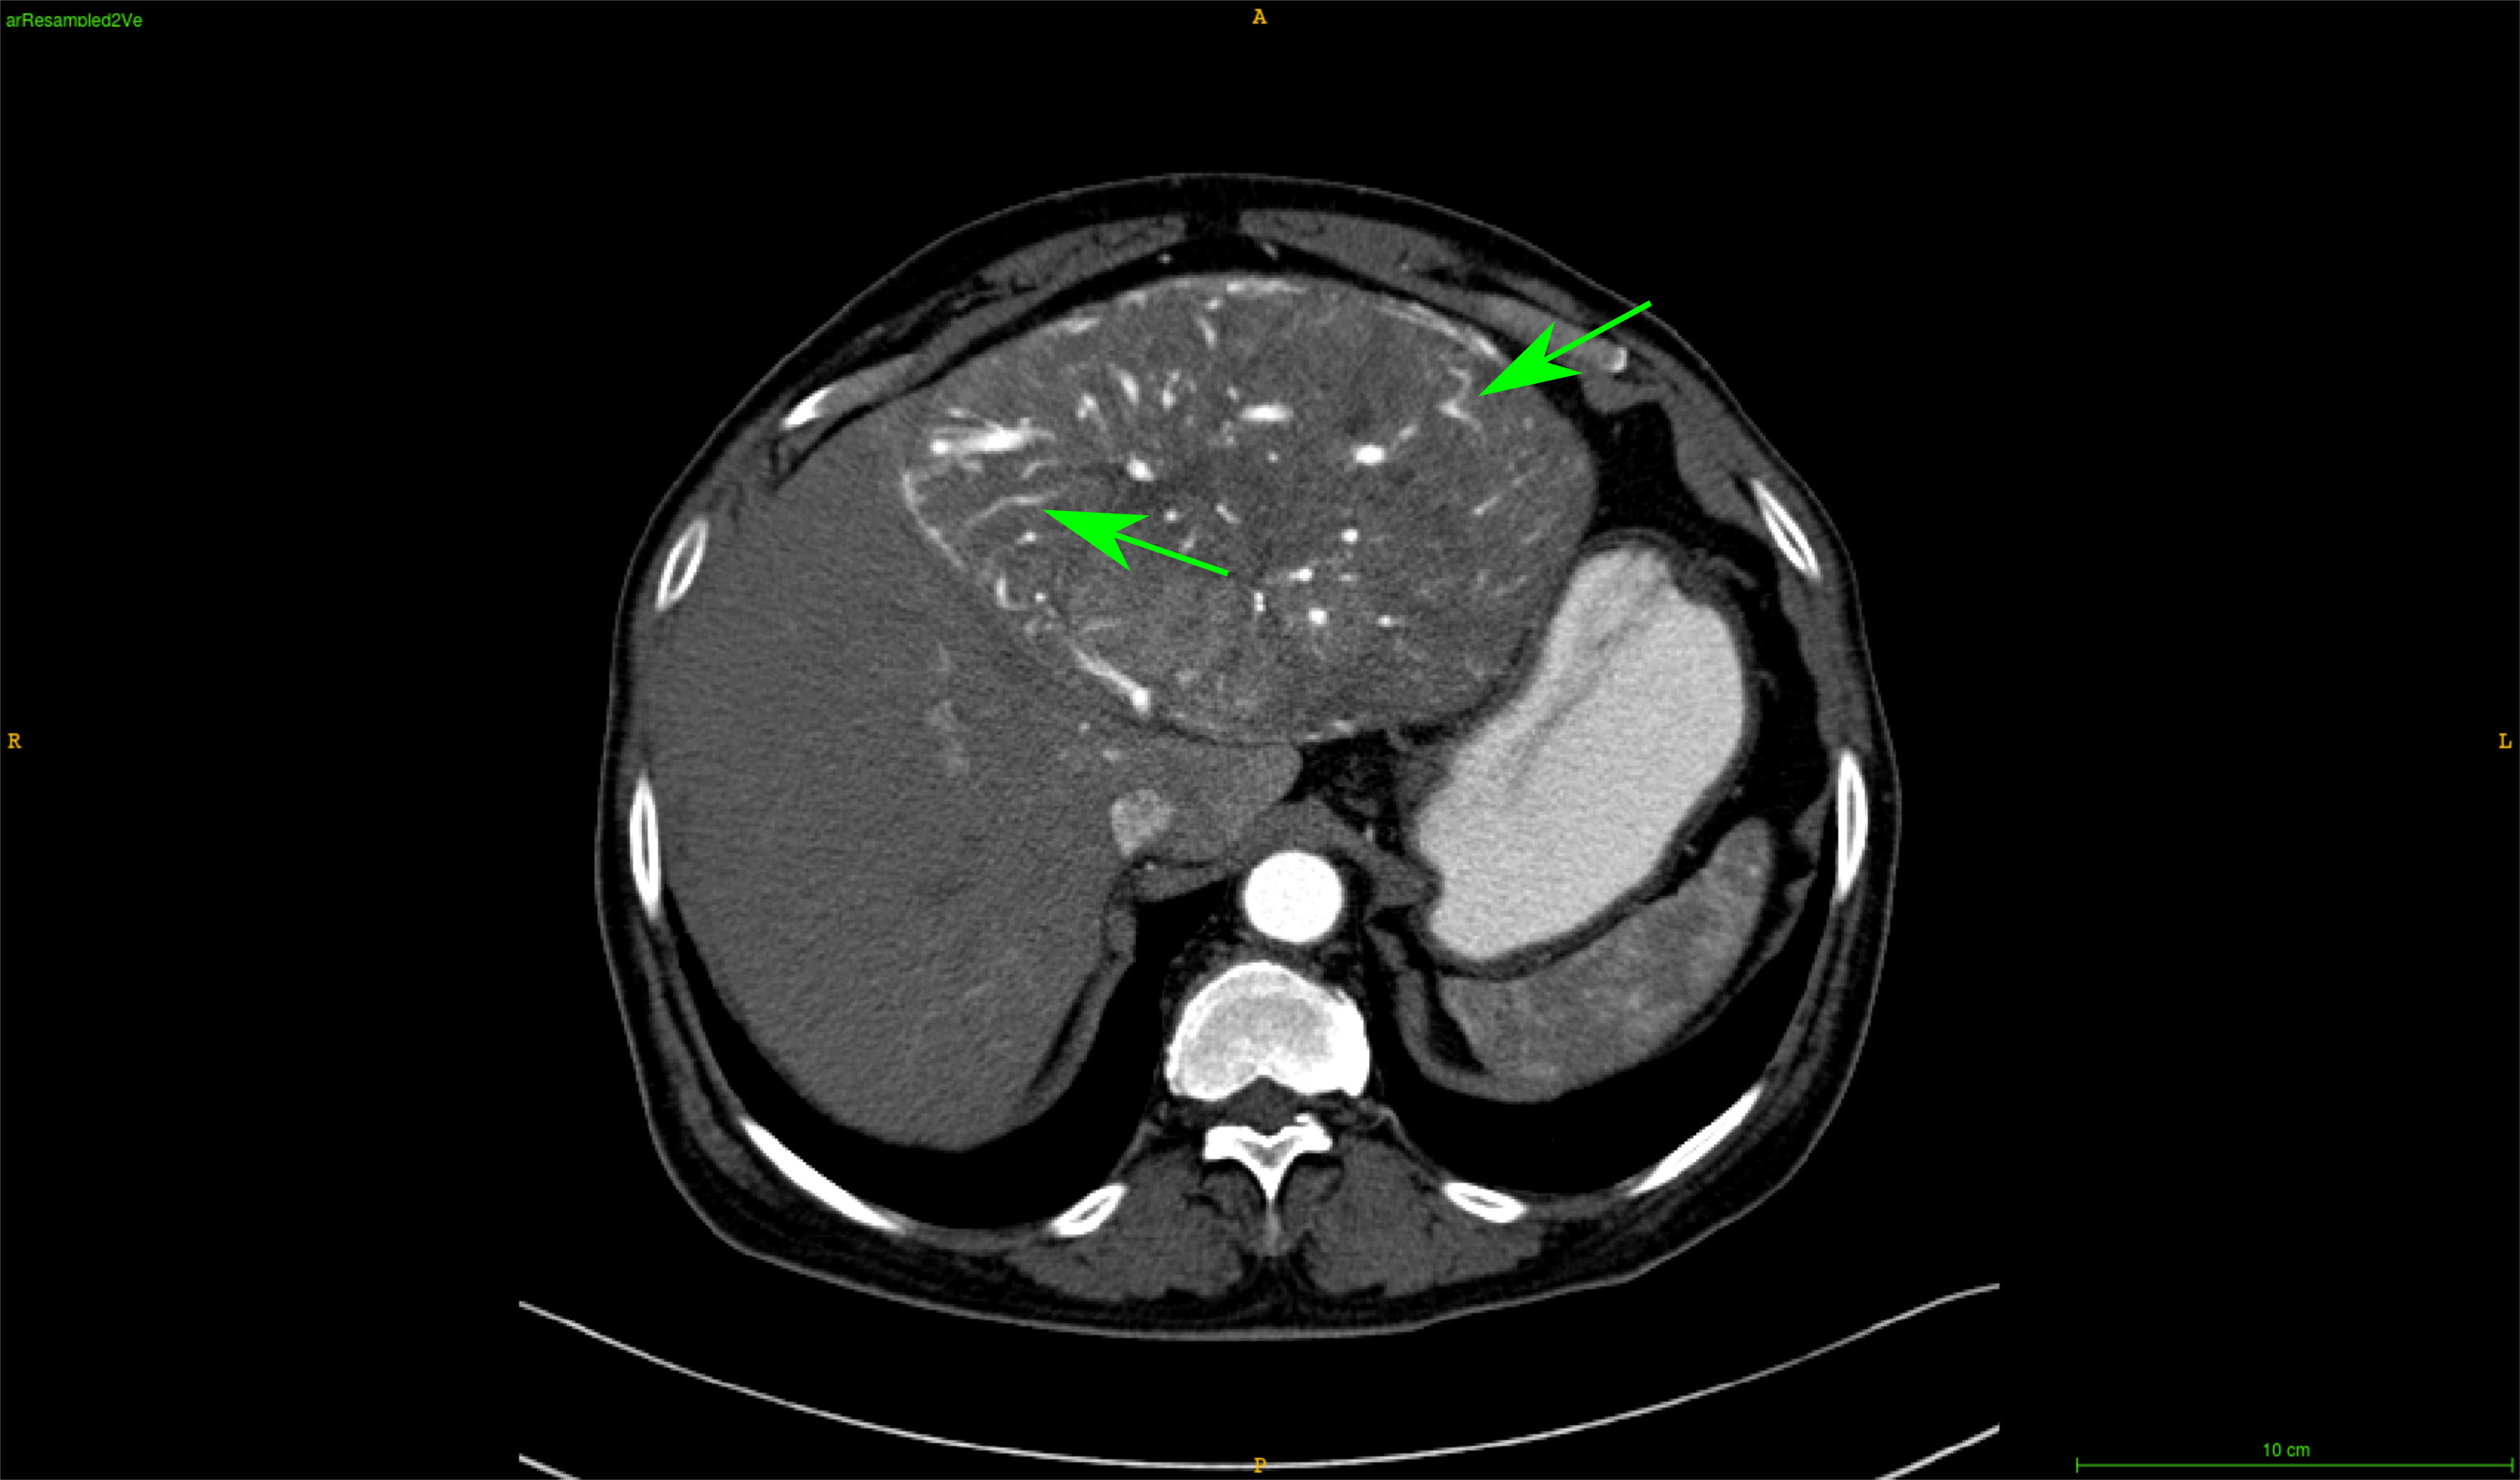
\includegraphics[width=\linewidth]{../Contributions/images/ImagingTraits/ResizeTCIA_internalArteries}
	\end{minipage} \\
	\begin{minipage}{0.45\linewidth}
		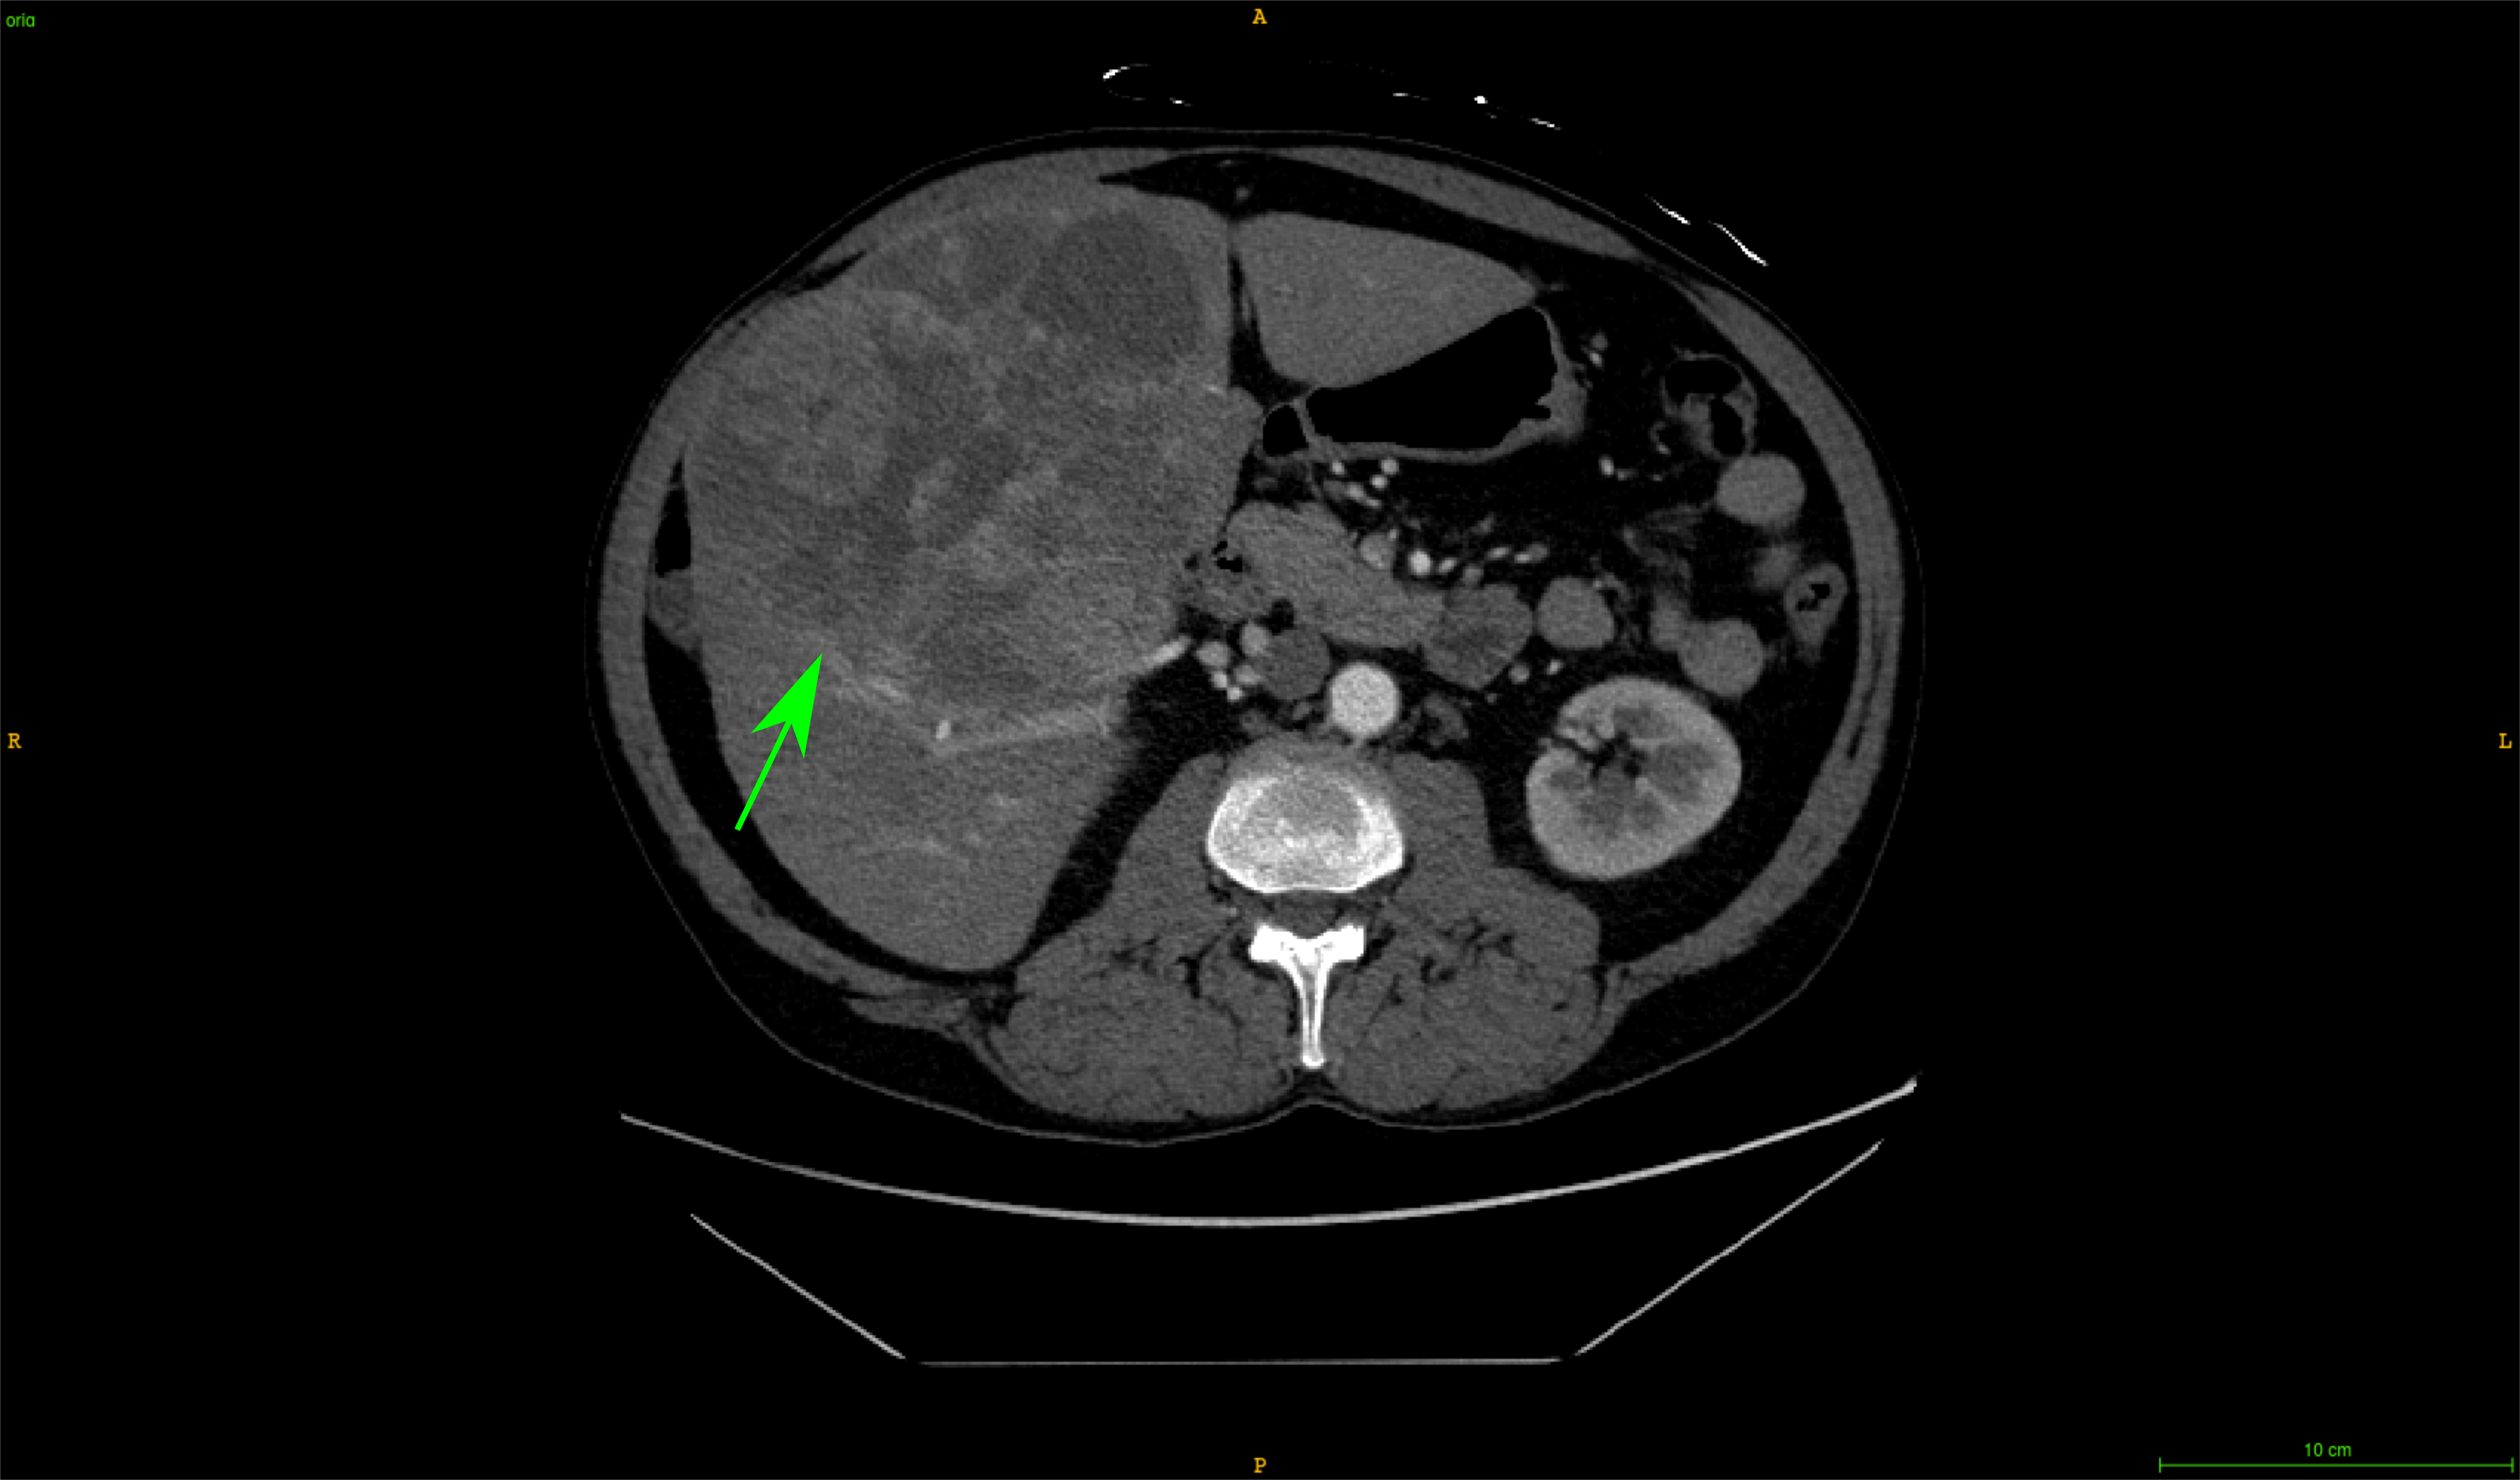
\includegraphics[width=\linewidth]{../Contributions/images/ImagingTraits/ResizeGDB_texturalHeterogeneity}
	\end{minipage} \hspace{-0.1cm}
	\begin{minipage}{0.45\linewidth}
		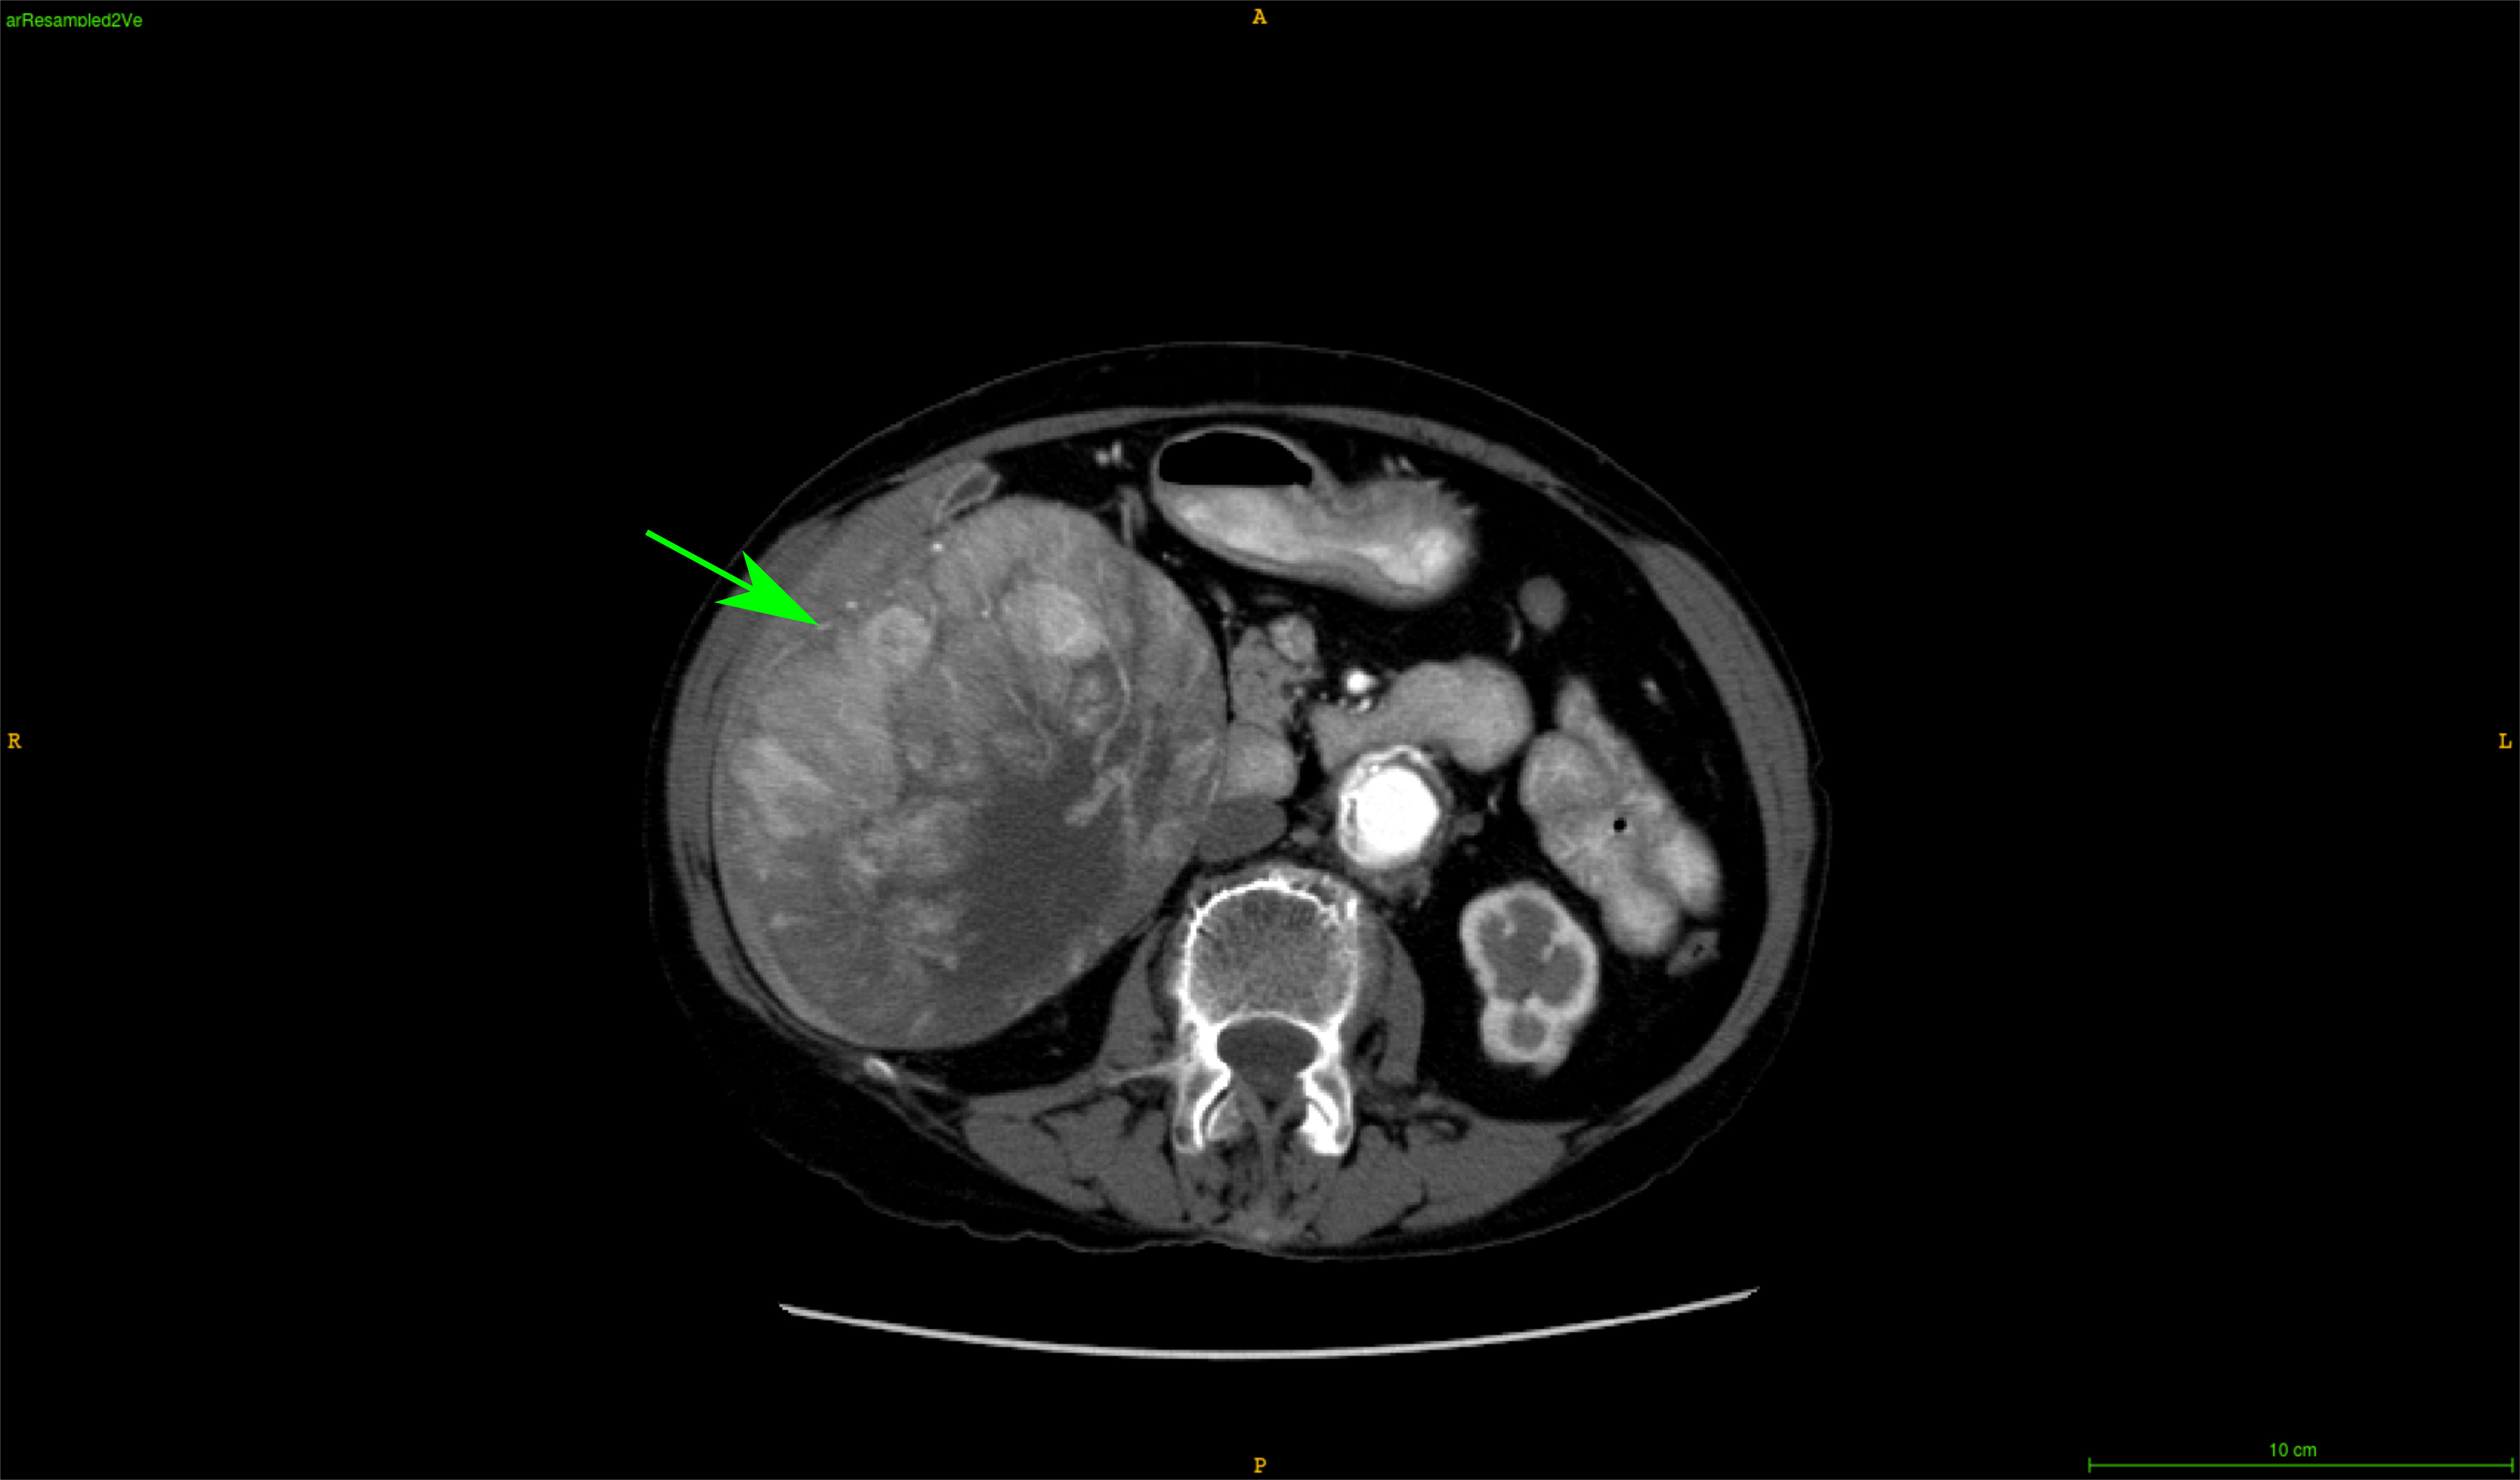
\includegraphics[width=\linewidth]{../Contributions/images/ImagingTraits/ResizeTCIA_texturalHeterogeneity}
	\end{minipage}
	\caption{Example of tumor characteristic imaging traits, relative to the inner part of the tumor, present in both training and test datasets. Left: \textbf{\lmttfont{G-dB}} images, right: \textbf{\lmttfont{TCIA-dB}} images. Top row: internal arteries, defined by the persistence of discrete arterial enhancement within the tumor in the \ac{ar} phase. Bottom row: high textural heterogeneity.}
	\label{fig:InterDb_imagingTraits2}
\end{figure}
\begin{figure}[!ht]
	\centering
	\begin{minipage}{0.45\linewidth}
		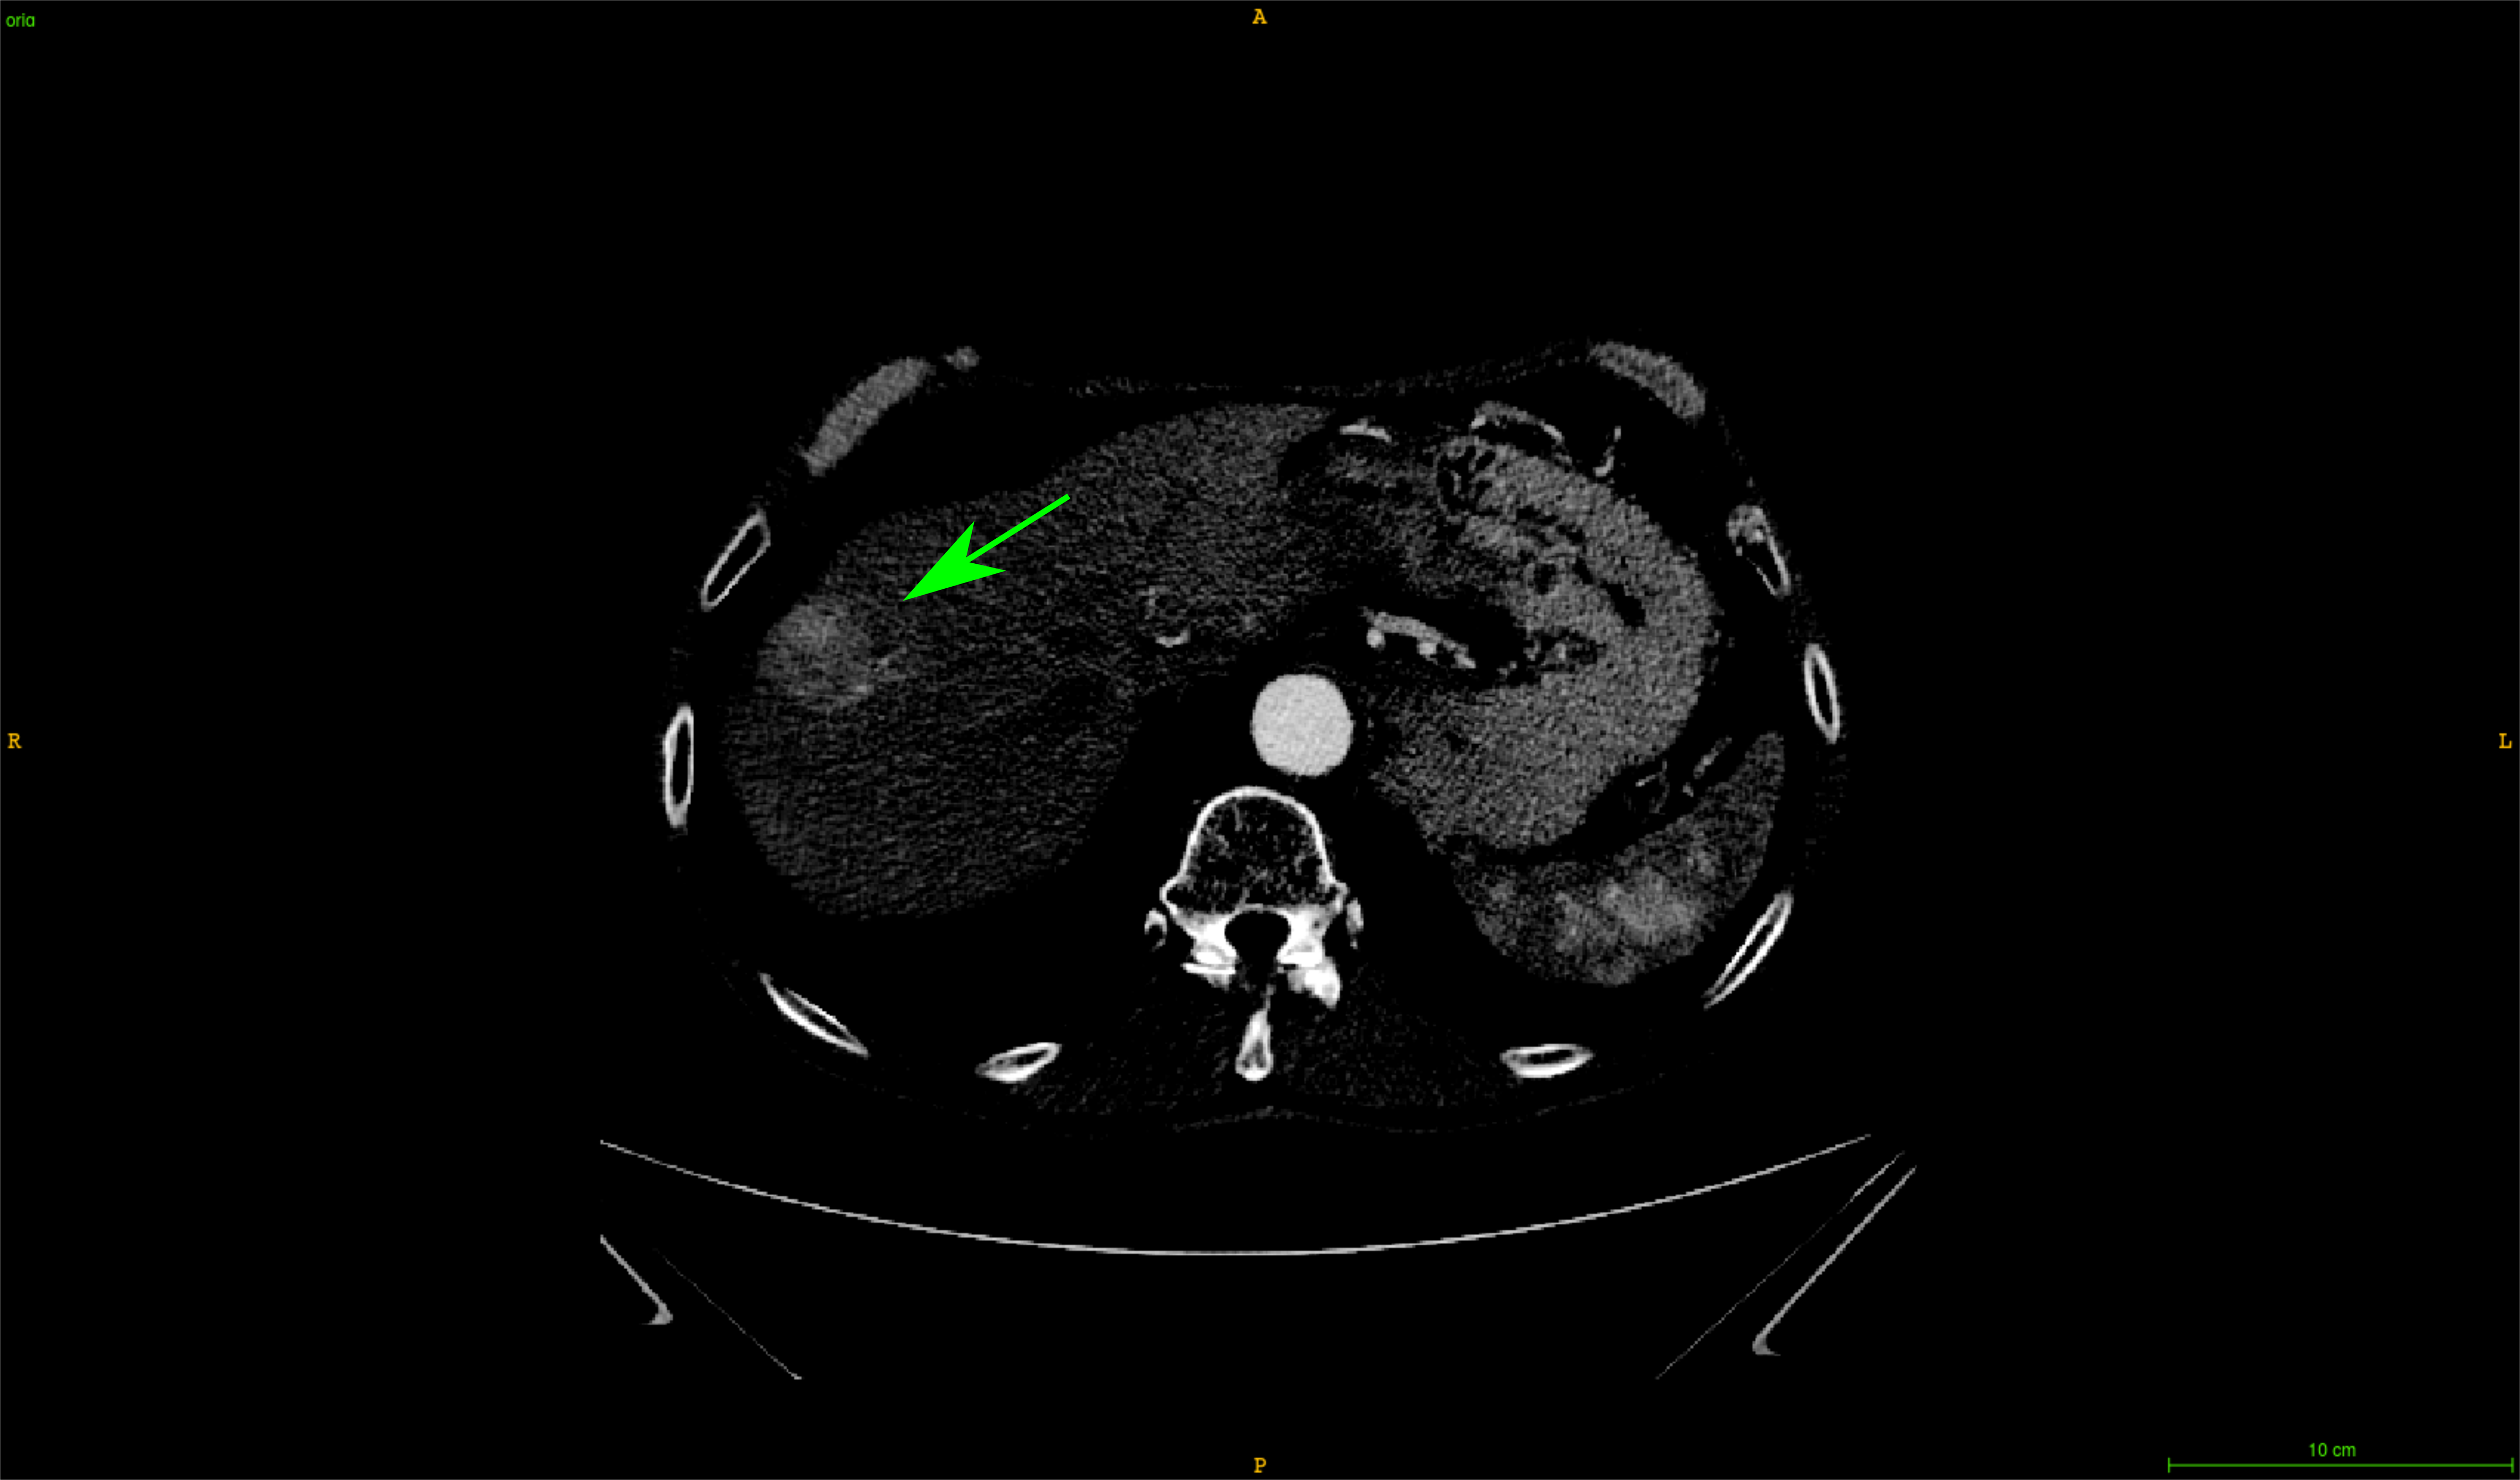
\includegraphics[width=\linewidth]{../Contributions/images/ImagingTraits/ResizeGDB_washin}
	\end{minipage} \hspace{-0.1cm}
	\begin{minipage}{0.45\linewidth}
		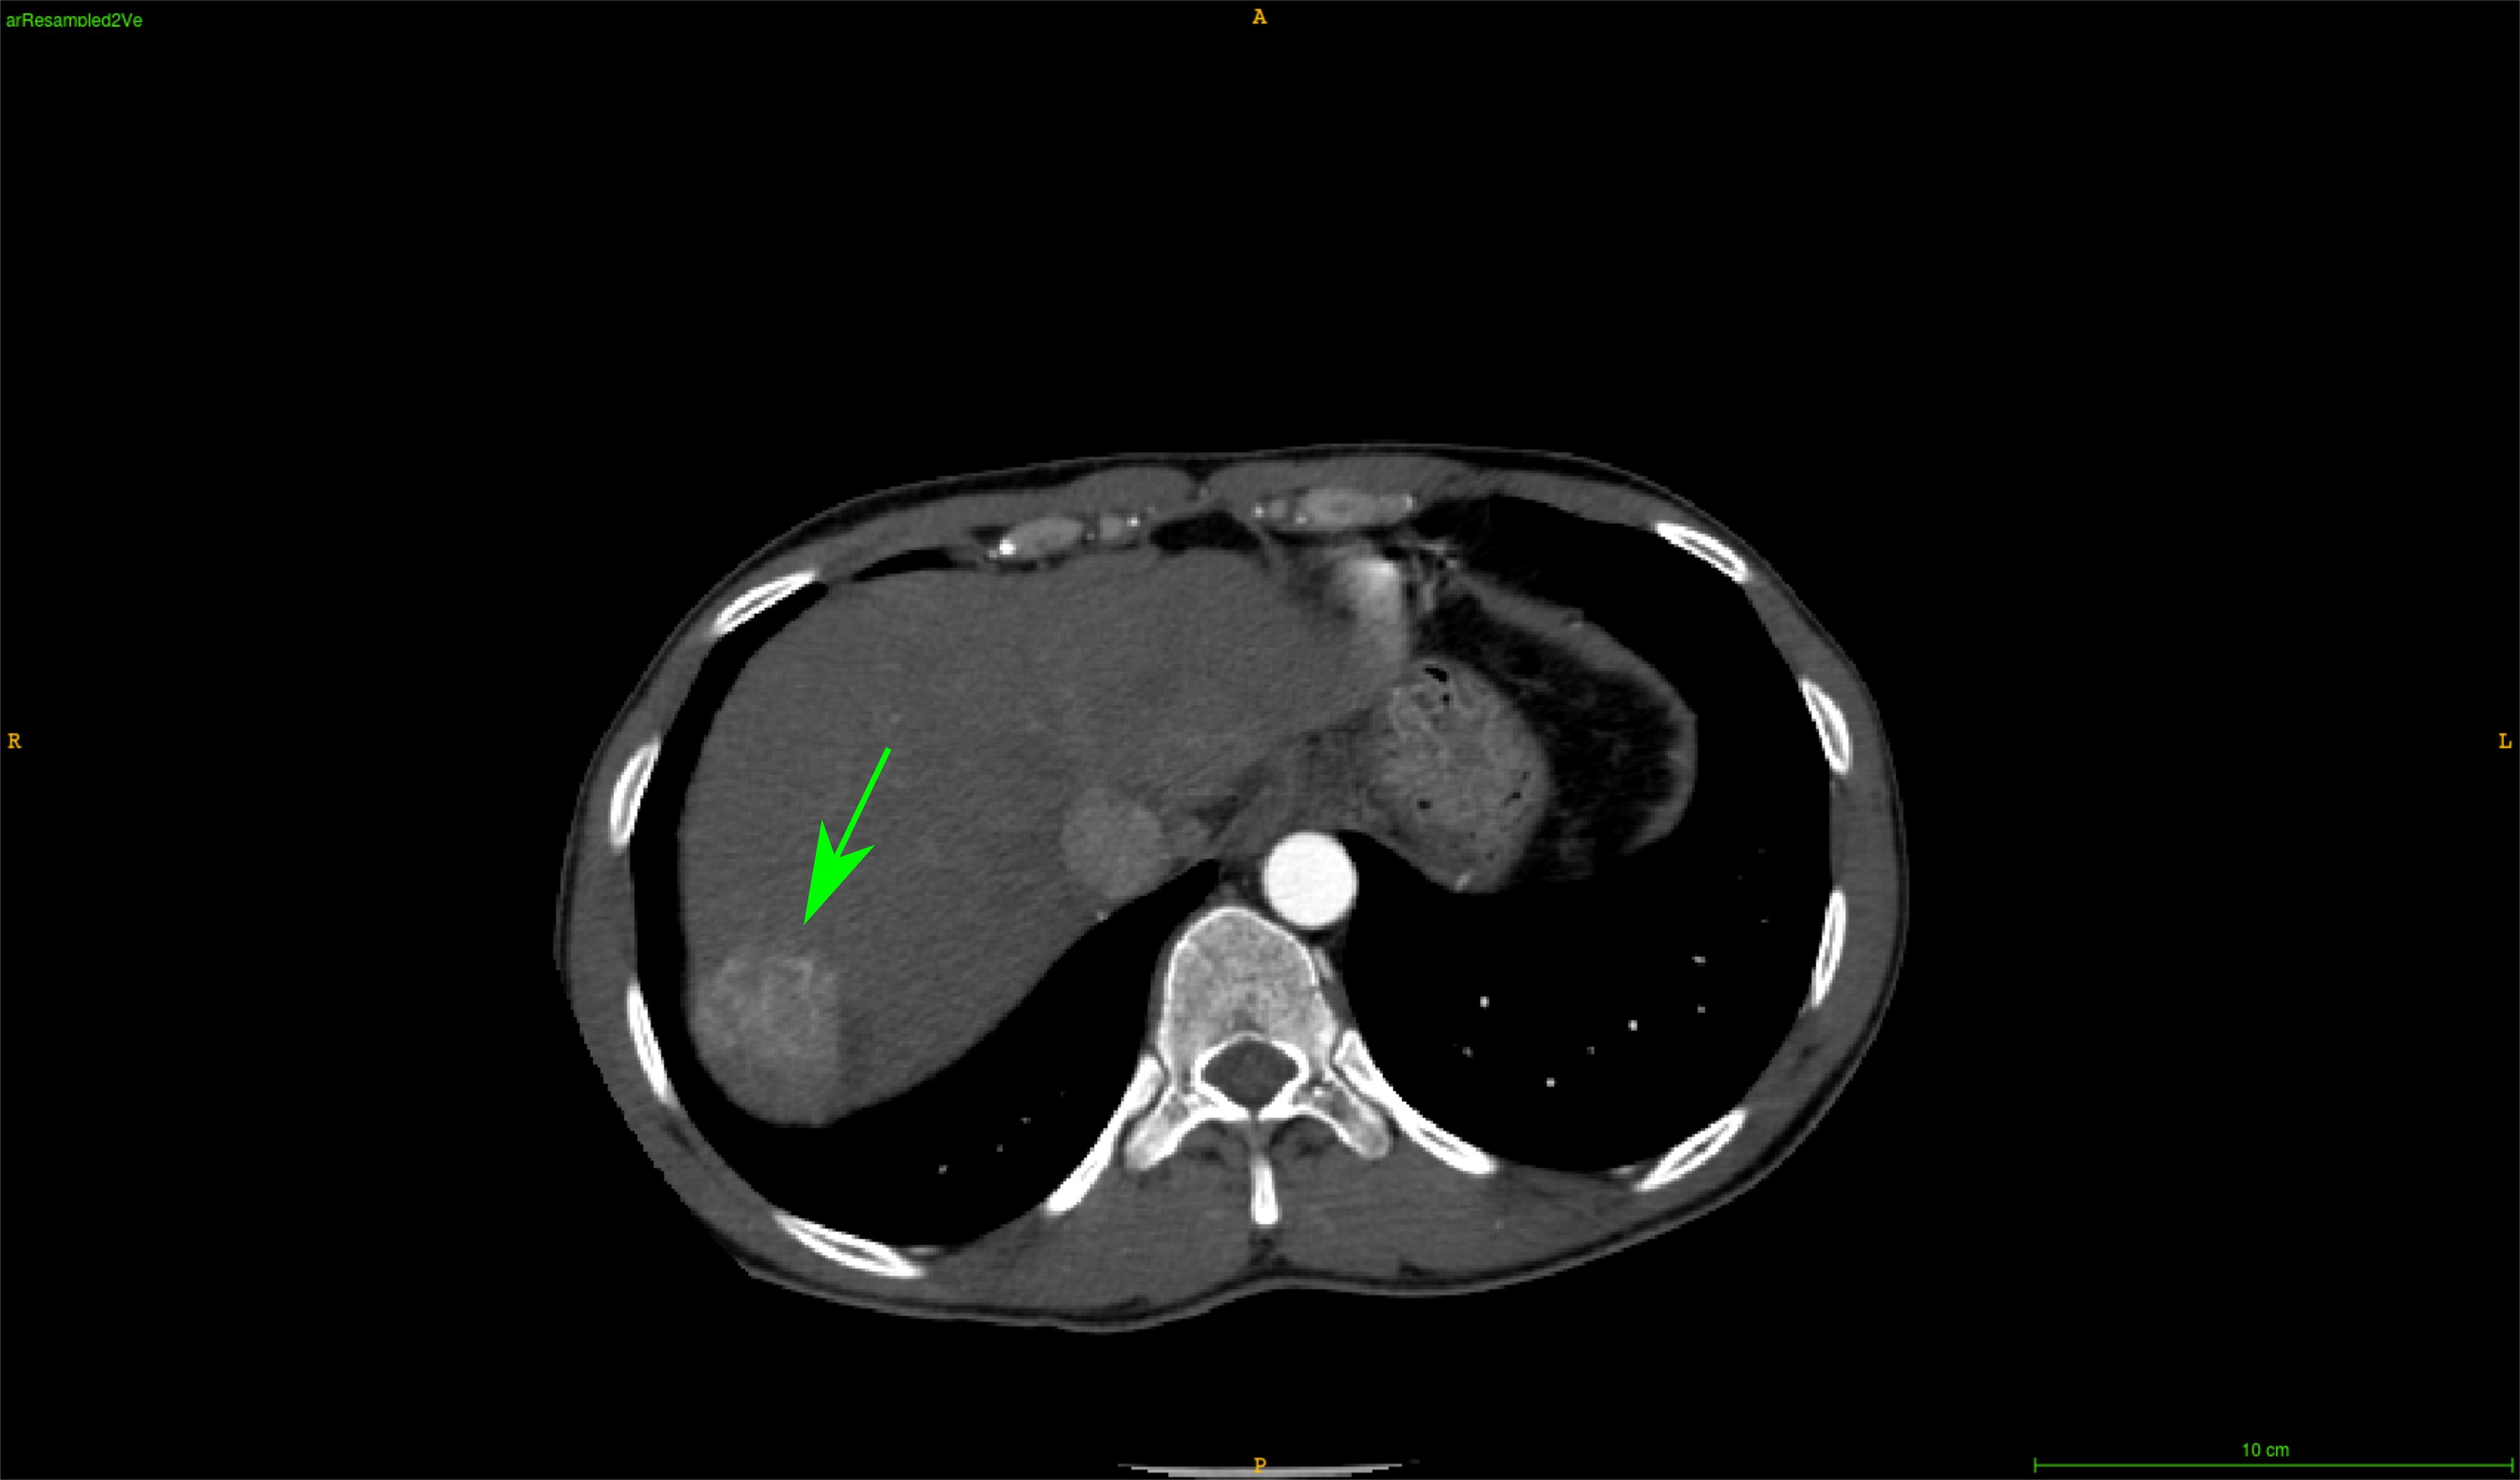
\includegraphics[width=\linewidth]{../Contributions/images/ImagingTraits/ResizeTCIA_washin}
	\end{minipage} \\
	\begin{minipage}{0.45\linewidth}
		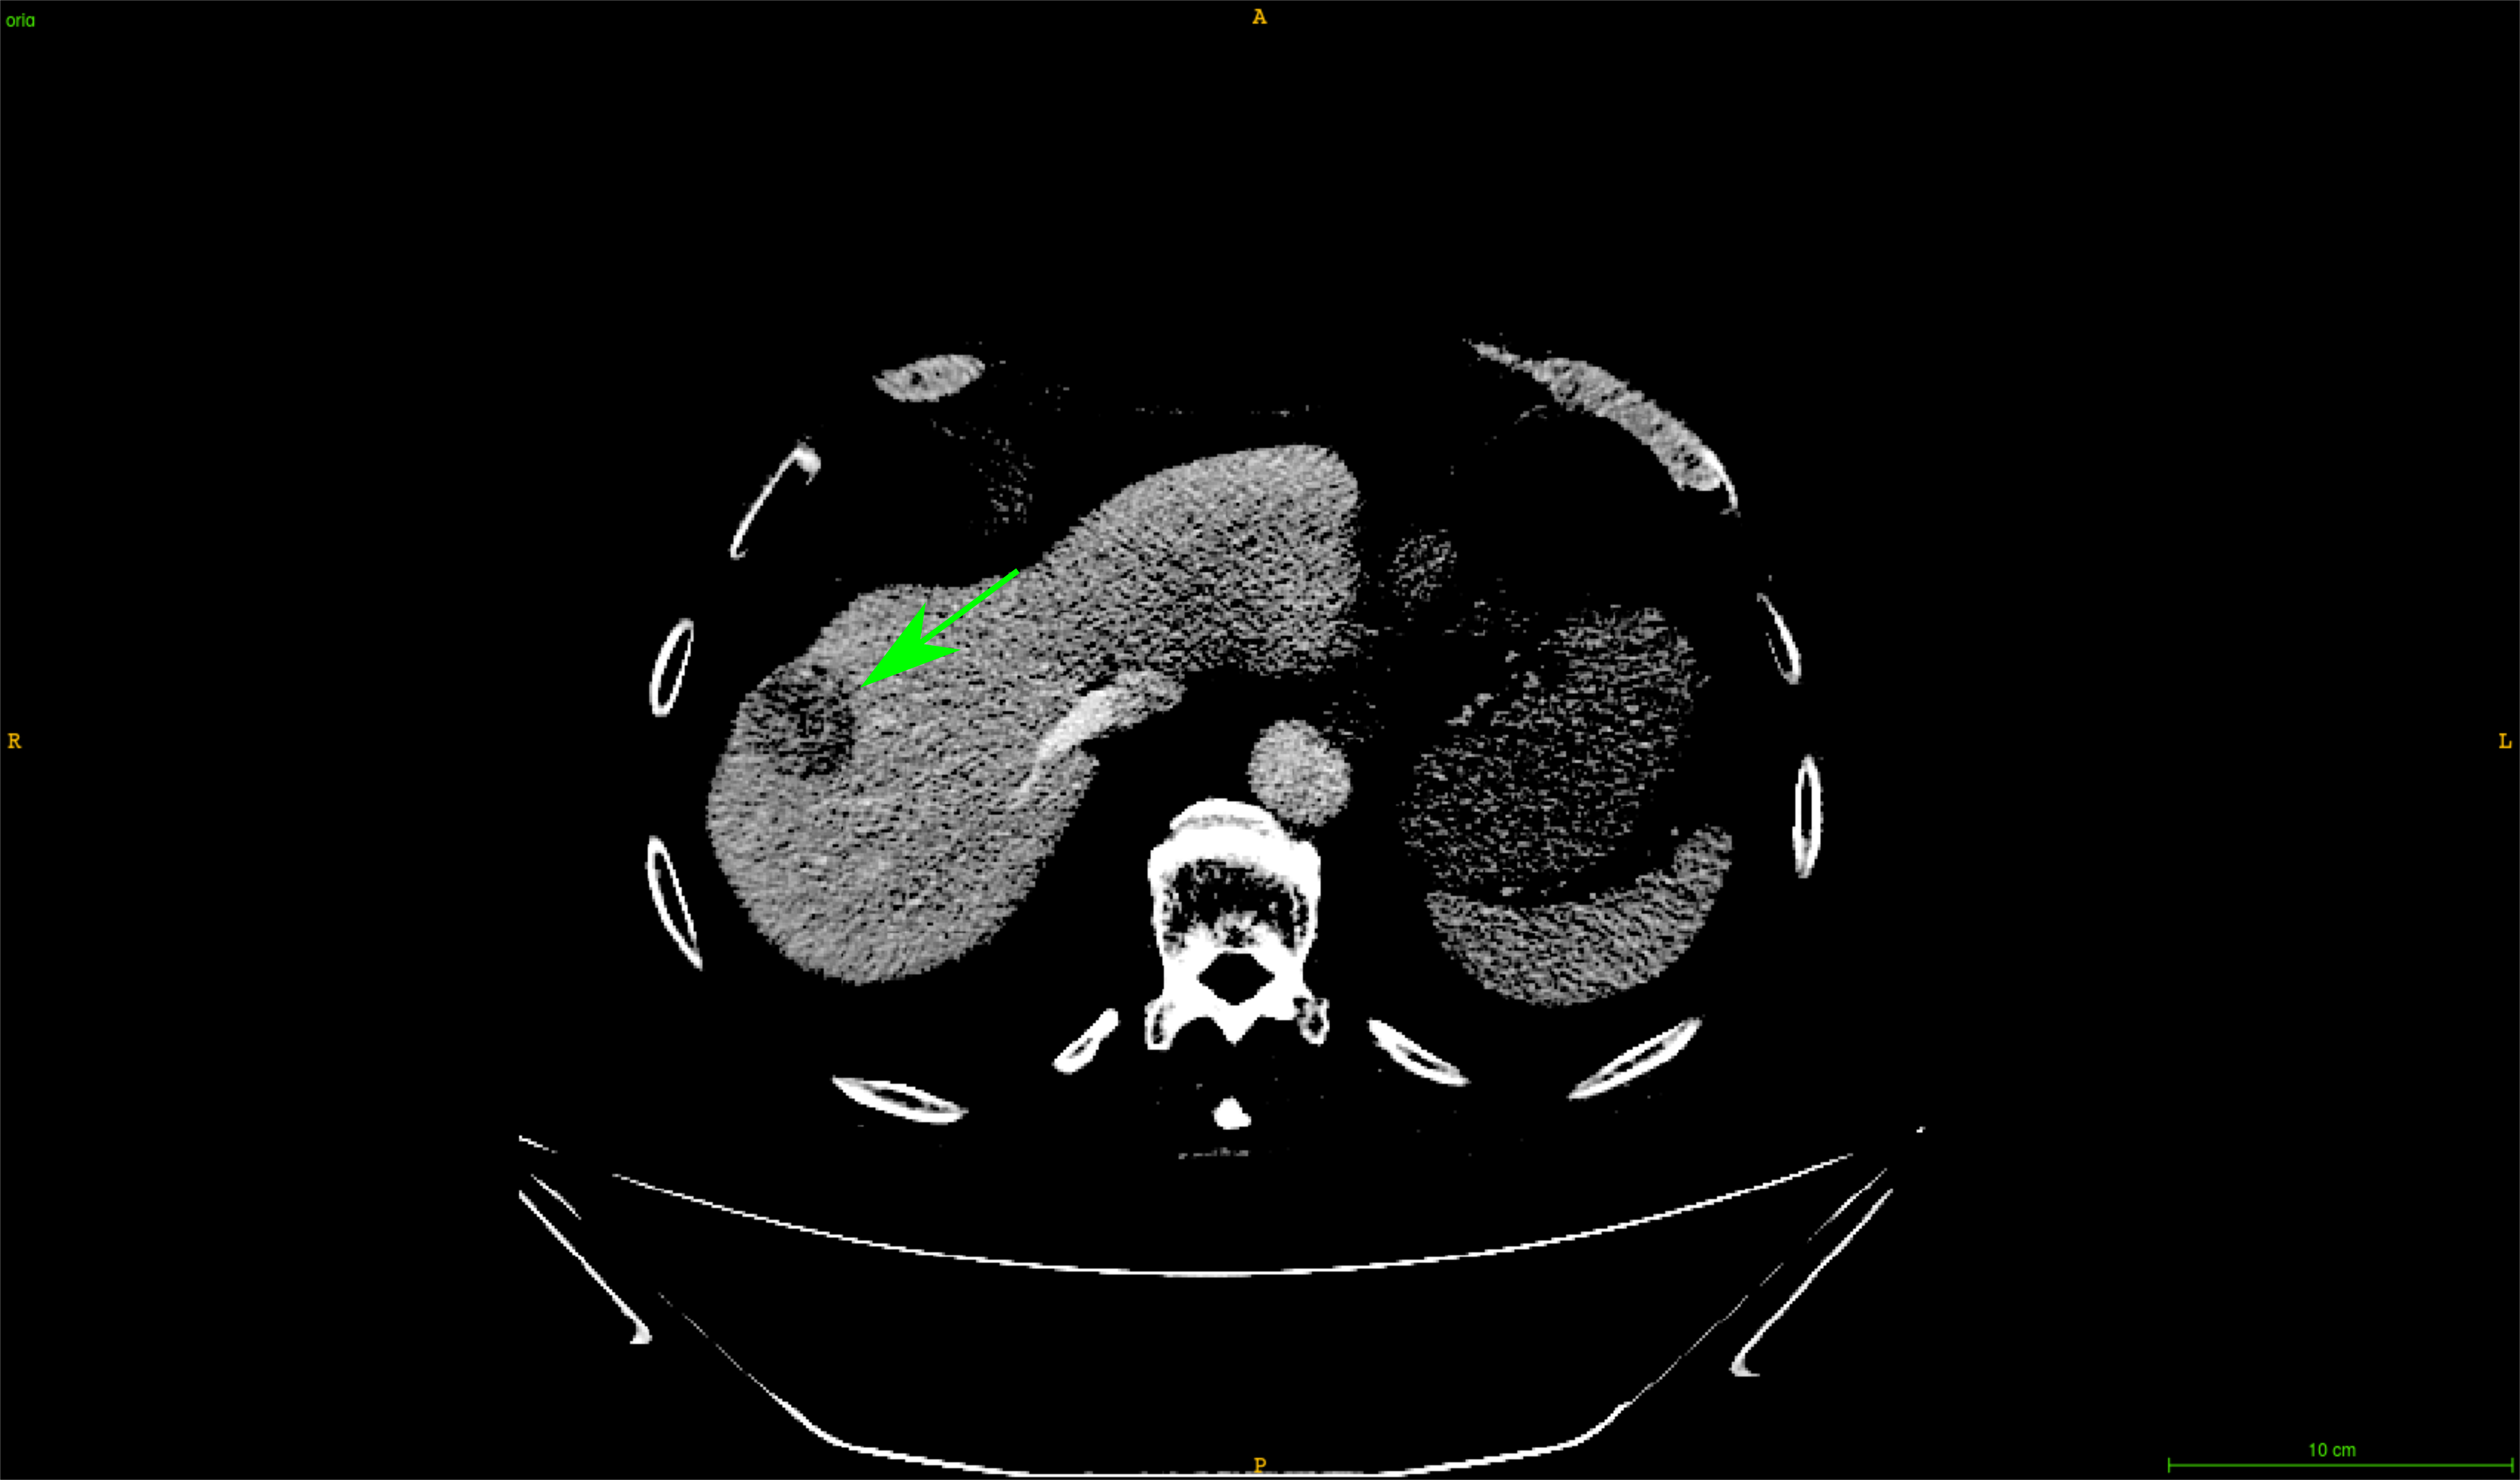
\includegraphics[width=\linewidth]{../Contributions/images/ImagingTraits/ResizeGDB_washout}
	\end{minipage} \hspace{-0.1cm}
	\begin{minipage}{0.45\linewidth}
		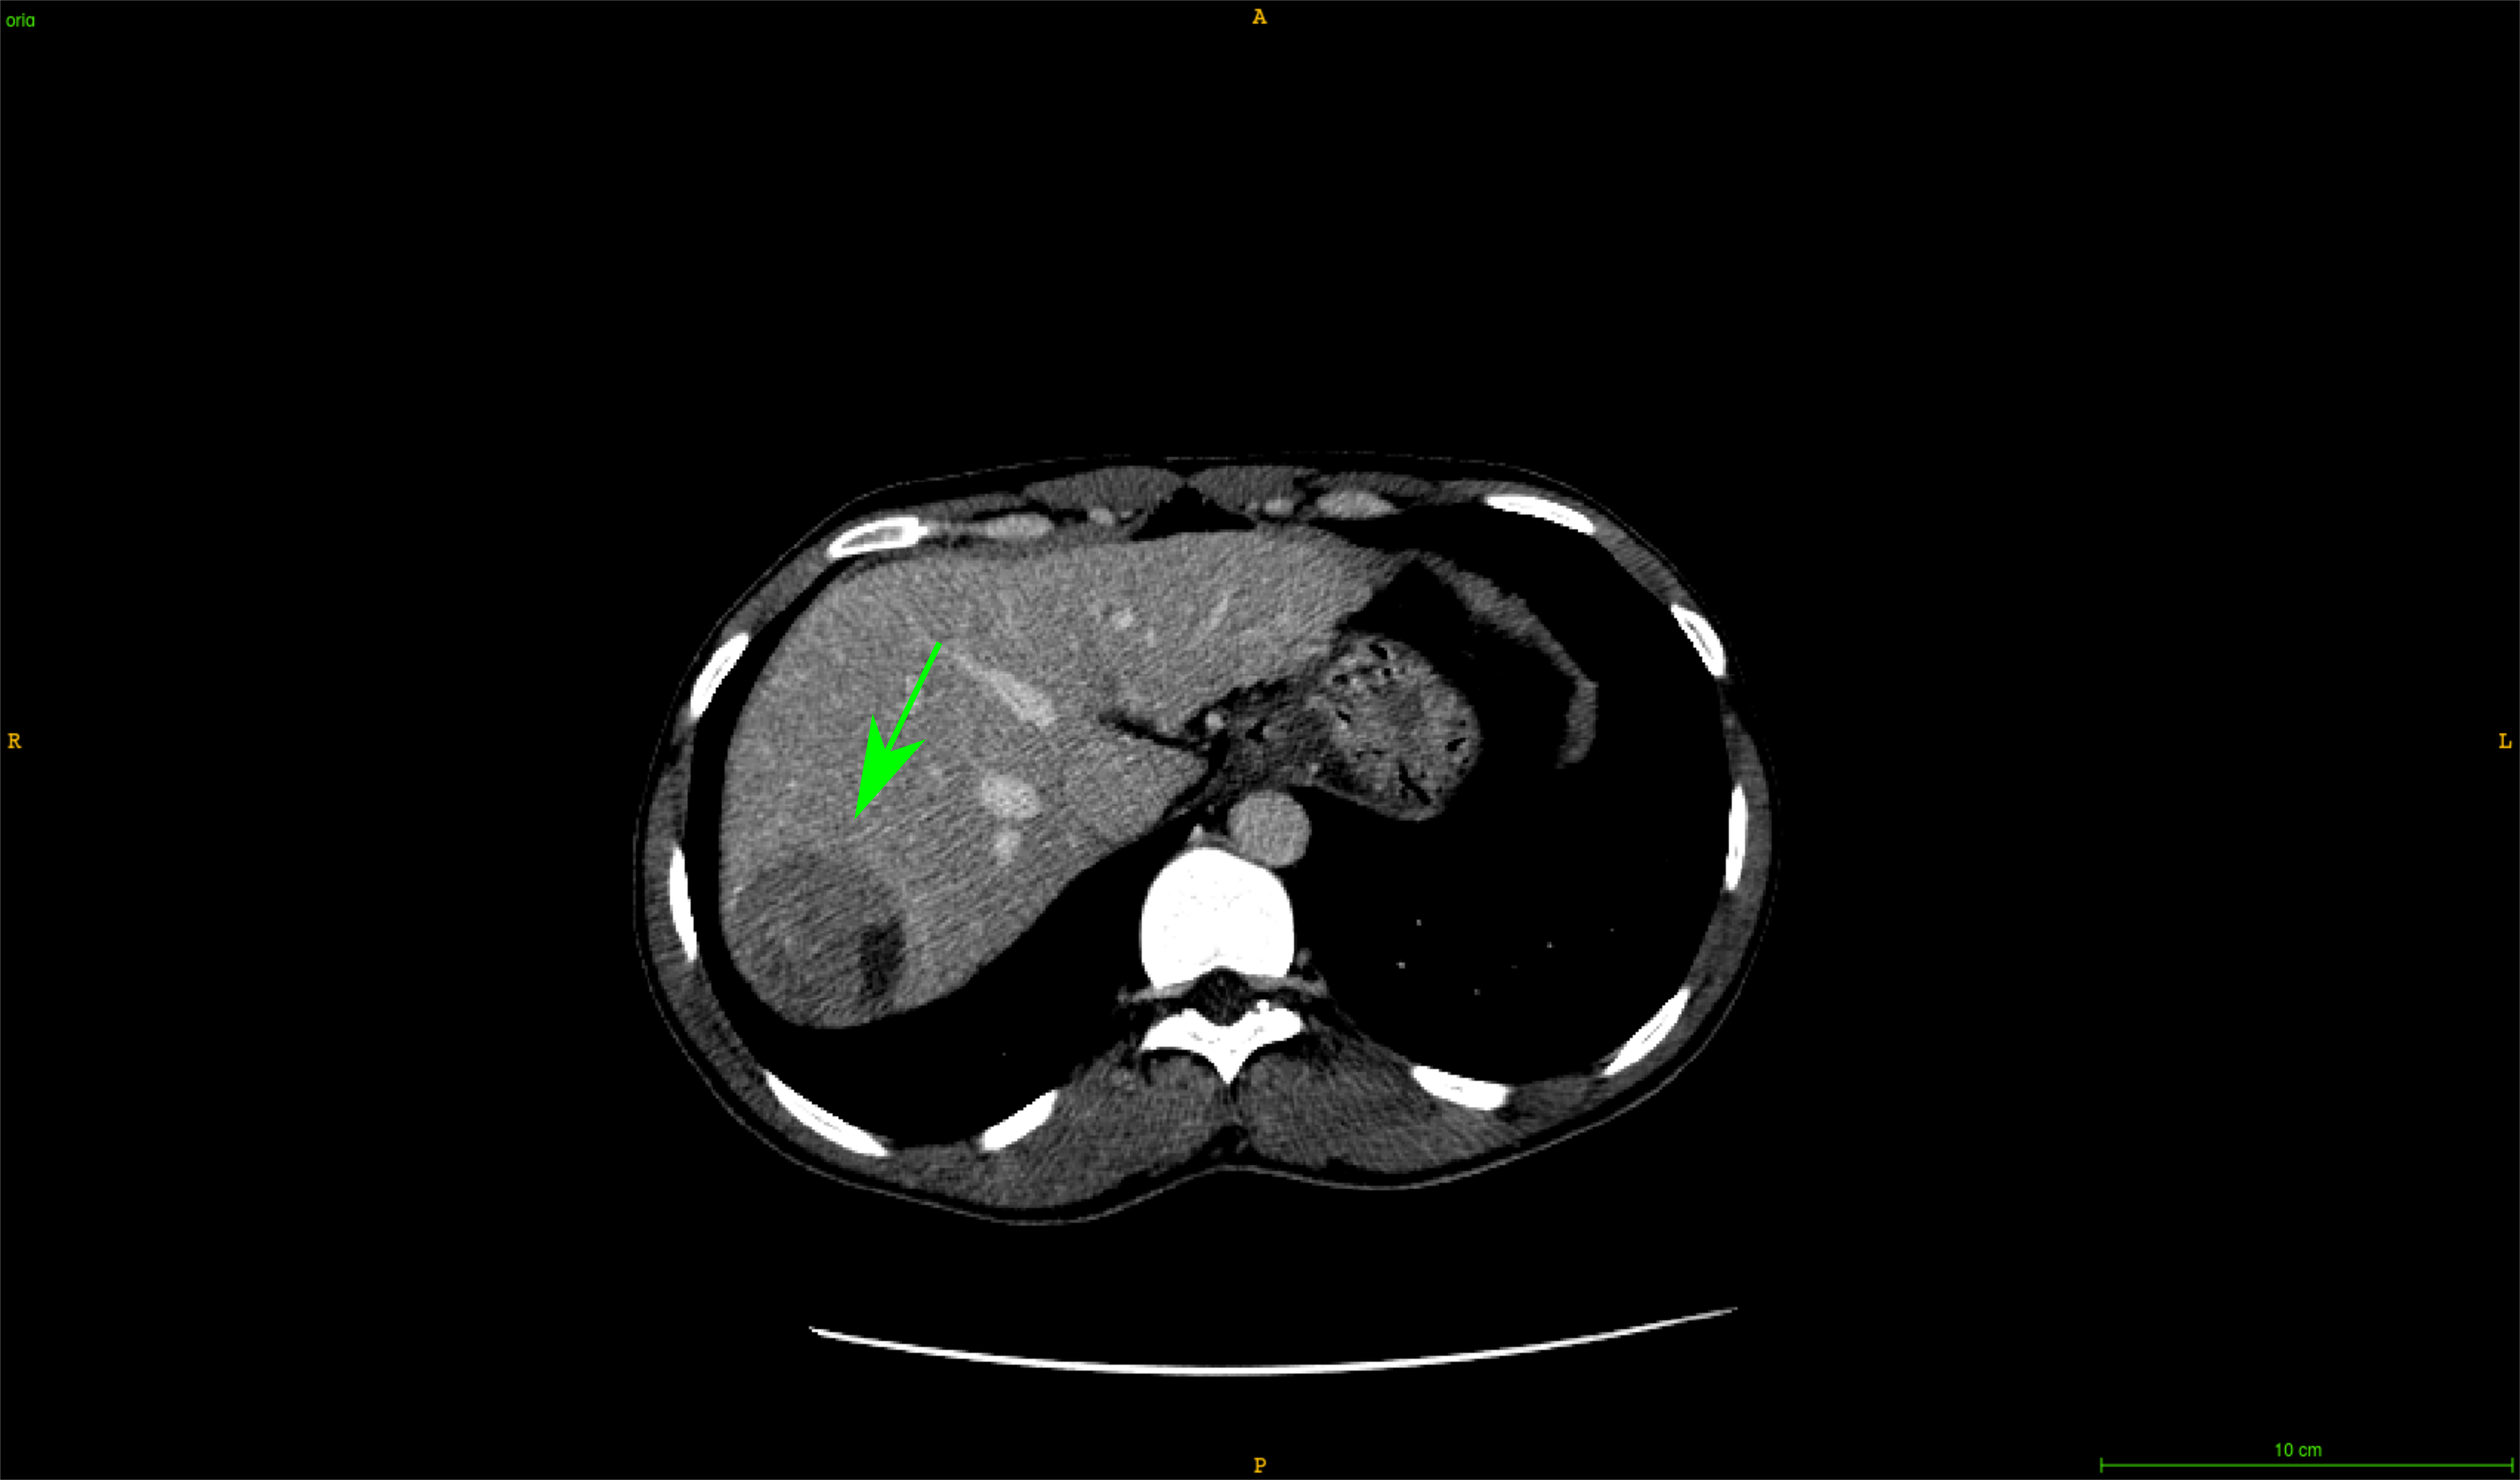
\includegraphics[width=\linewidth]{../Contributions/images/ImagingTraits/ResizeTCIA_washout}
	\end{minipage}
	\caption{Example of specific wash-in/wash-out trait present in both training and test datasets. Left: \textbf{\lmttfont{G-dB}} images, right: \textbf{\lmttfont{TCIA-dB}} images.
	Wash-in is defined as an enhancement of the lesion of the arterial phase higher than the one of the liver parenchyma, whereas the wash-out is defined as a lesion hypodense/hypointense compared to the liver parenchyma on the portal venous and/or delayed phases.}
	\label{fig:InterDb_imagingTraits3}
\end{figure}


The same quantitative analysis as previously was performed (see section \textcolor{red}{\textbf{ref above section}}), with the placement of 5 ROIs in randomly chosen patients of both the training (\textbf{\lmttfont{G-dB}}) and the testing (\textbf{\lmttfont{TCIA-dB}}) datasets. ROIs were placed in the liver parenchyma, the air, the spleen, the bone and the aorta. These areas were chosen mainly to detect potential cirrhotic patients in both datasets, as illustrated in the figure \ref{fig:cirrhoticPatPlot}, and to assess the homogeneity for the given phases among the different datasets, as depicted in the figure \ref{fig:gdbAortaPlot}. 
\begin{figure}[!ht]
	\centering
	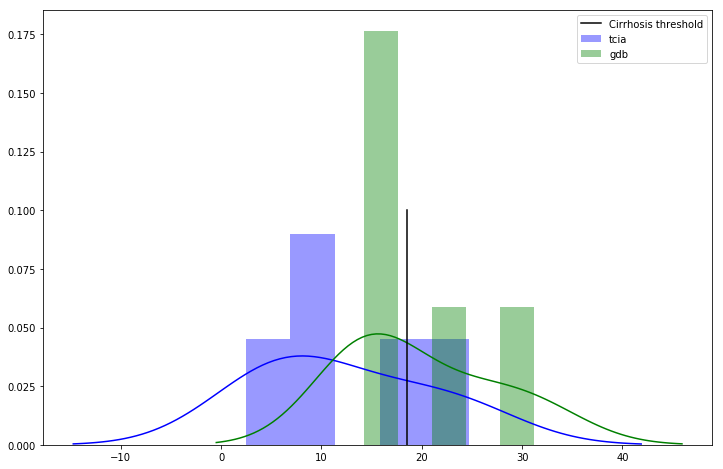
\includegraphics[width=0.6\linewidth]{../Contributions/images/Gdb_TCIA_cirrhosisPlot_bins5}
	\caption{Histogram representing the distribution of the difference between parenchyma and spleen intensities for the patients of  \textbf{\lmttfont{G-dB}} dataset (green) and the  \textbf{\lmttfont{TCIA-dB}} dataset (blue). A difference higher than 18.5 HU (black vertical line) can be a sign of cirrhosis.
	}
	\label{fig:cirrhoticPatPlot}
\end{figure}
\begin{figure}[!ht]
	\centering
	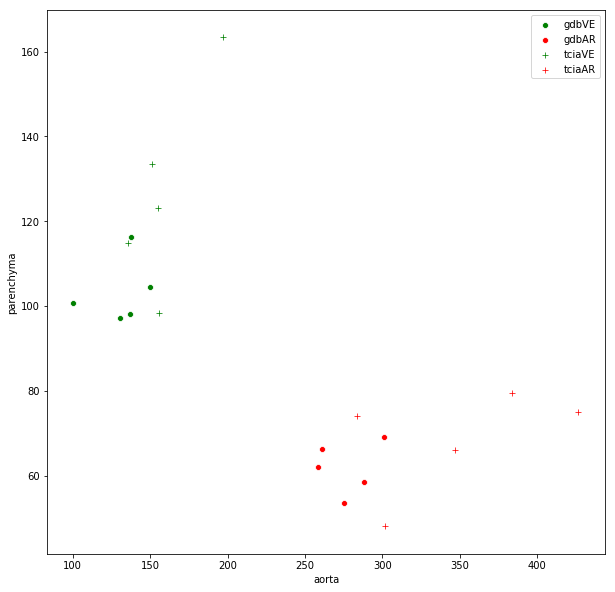
\includegraphics[width=0.6\linewidth]{../Contributions/images/AortaParPlot_Gdb_2}
	\caption{Mean aorta intensity vs mean liver parenchyma intensity. Each point represents one volume. We can see a clear separation between arterial (red) and portal venous (green) volumes for both the \textbf{\lmttfont{G-dB}} and the \textbf{\lmttfont{TCIA-dB}} patients. We can however notice a higher heterogeneity among the mean parenchyma intensity in the \textbf{\lmttfont{TCIA-dB}} dataset, which could be a sign of standardize acquisition settings within the \textbf{\lmttfont{G-dB}}.
	}
	\label{fig:gdbAortaPlot}
\end{figure}


\subsection{Histological grade dataset}

Regarding the histological grade prediction, both the training and the testing steps have been performed on the \textbf{\lmttfont{TCIA-dB}} dataset in a cross-validation manner.
This dataset contains images from 18 patients, where 9 were diagnosed 
with a grade 3 (G3), 7 with a grade 2 (G2) and 2 with a grade 1 (G1). In order
to obtain a balanced dataset, it has been decided to split them
into two groups, the first containing G1 and G2 patients, and the second containing G3 patients, as it has been done previously in the literature since G2
was considered as being closer to G1 than to G3 \cite{Han2013,Zucman-Rossi2015}. Patients from the first group (G1 and G2) were considered as
having a low grade (LG), whereas those from the second group have a high
grade (HG).


\section{Methods}

In this section, we present our cascaded automatic liver tumor segmentation architecture, inspired from the one implemented in the section \todo{Add ref IJCARS section}, especially our so-called \pplfont{\ac{cect}-Liver}, responsible for the automatic segmentation of liver on both \ac{ar} and \ac{pv} volumes. We then present both the \ac{hcr}-based and the \ac{dlr}-based histological grade prediction networks.


\subsection{Automatic liver tumor segmentation} \label{subsect_auto_liver_tumor_seg}

Our cascaded liver tumor segmentation architecture is composed of one \pplfont{\ac{cect}-Liver} network, presented hereafter, followed by a multiphase tumor segmentation network (both the \pplfont{MPF-Tumor} and the \pplfont{DMP-Tumor} networks were trained and their accuracy compared), already presented in the section \todo{add ref}. \\
We trained our network called \pplfont{\ac{cect}-Liver} on the 131 volumes of the
\textbf{\lmttfont{LITS-dB}} using the same hyperparameters as the ones detailed
previously. The network shares the same settings as the previously defined \pplfont{\ac{pv}-Liver} and \pplfont{\ac{ar}-Liver} networks (see figure \ref{fig:CECTliverDetails}). In this case we used the architecture with 1024 filters at bottleneck, corresponding to about 32M parameters. Once the segmentation is performed on each of the axial slices of a given patient, we implemented 2 post-processing steps by first extracting the biggest connected component in the entire 3D volume before applying a binary opening operation to the retained mask.
\begin{figure}[!ht]
	\centering
	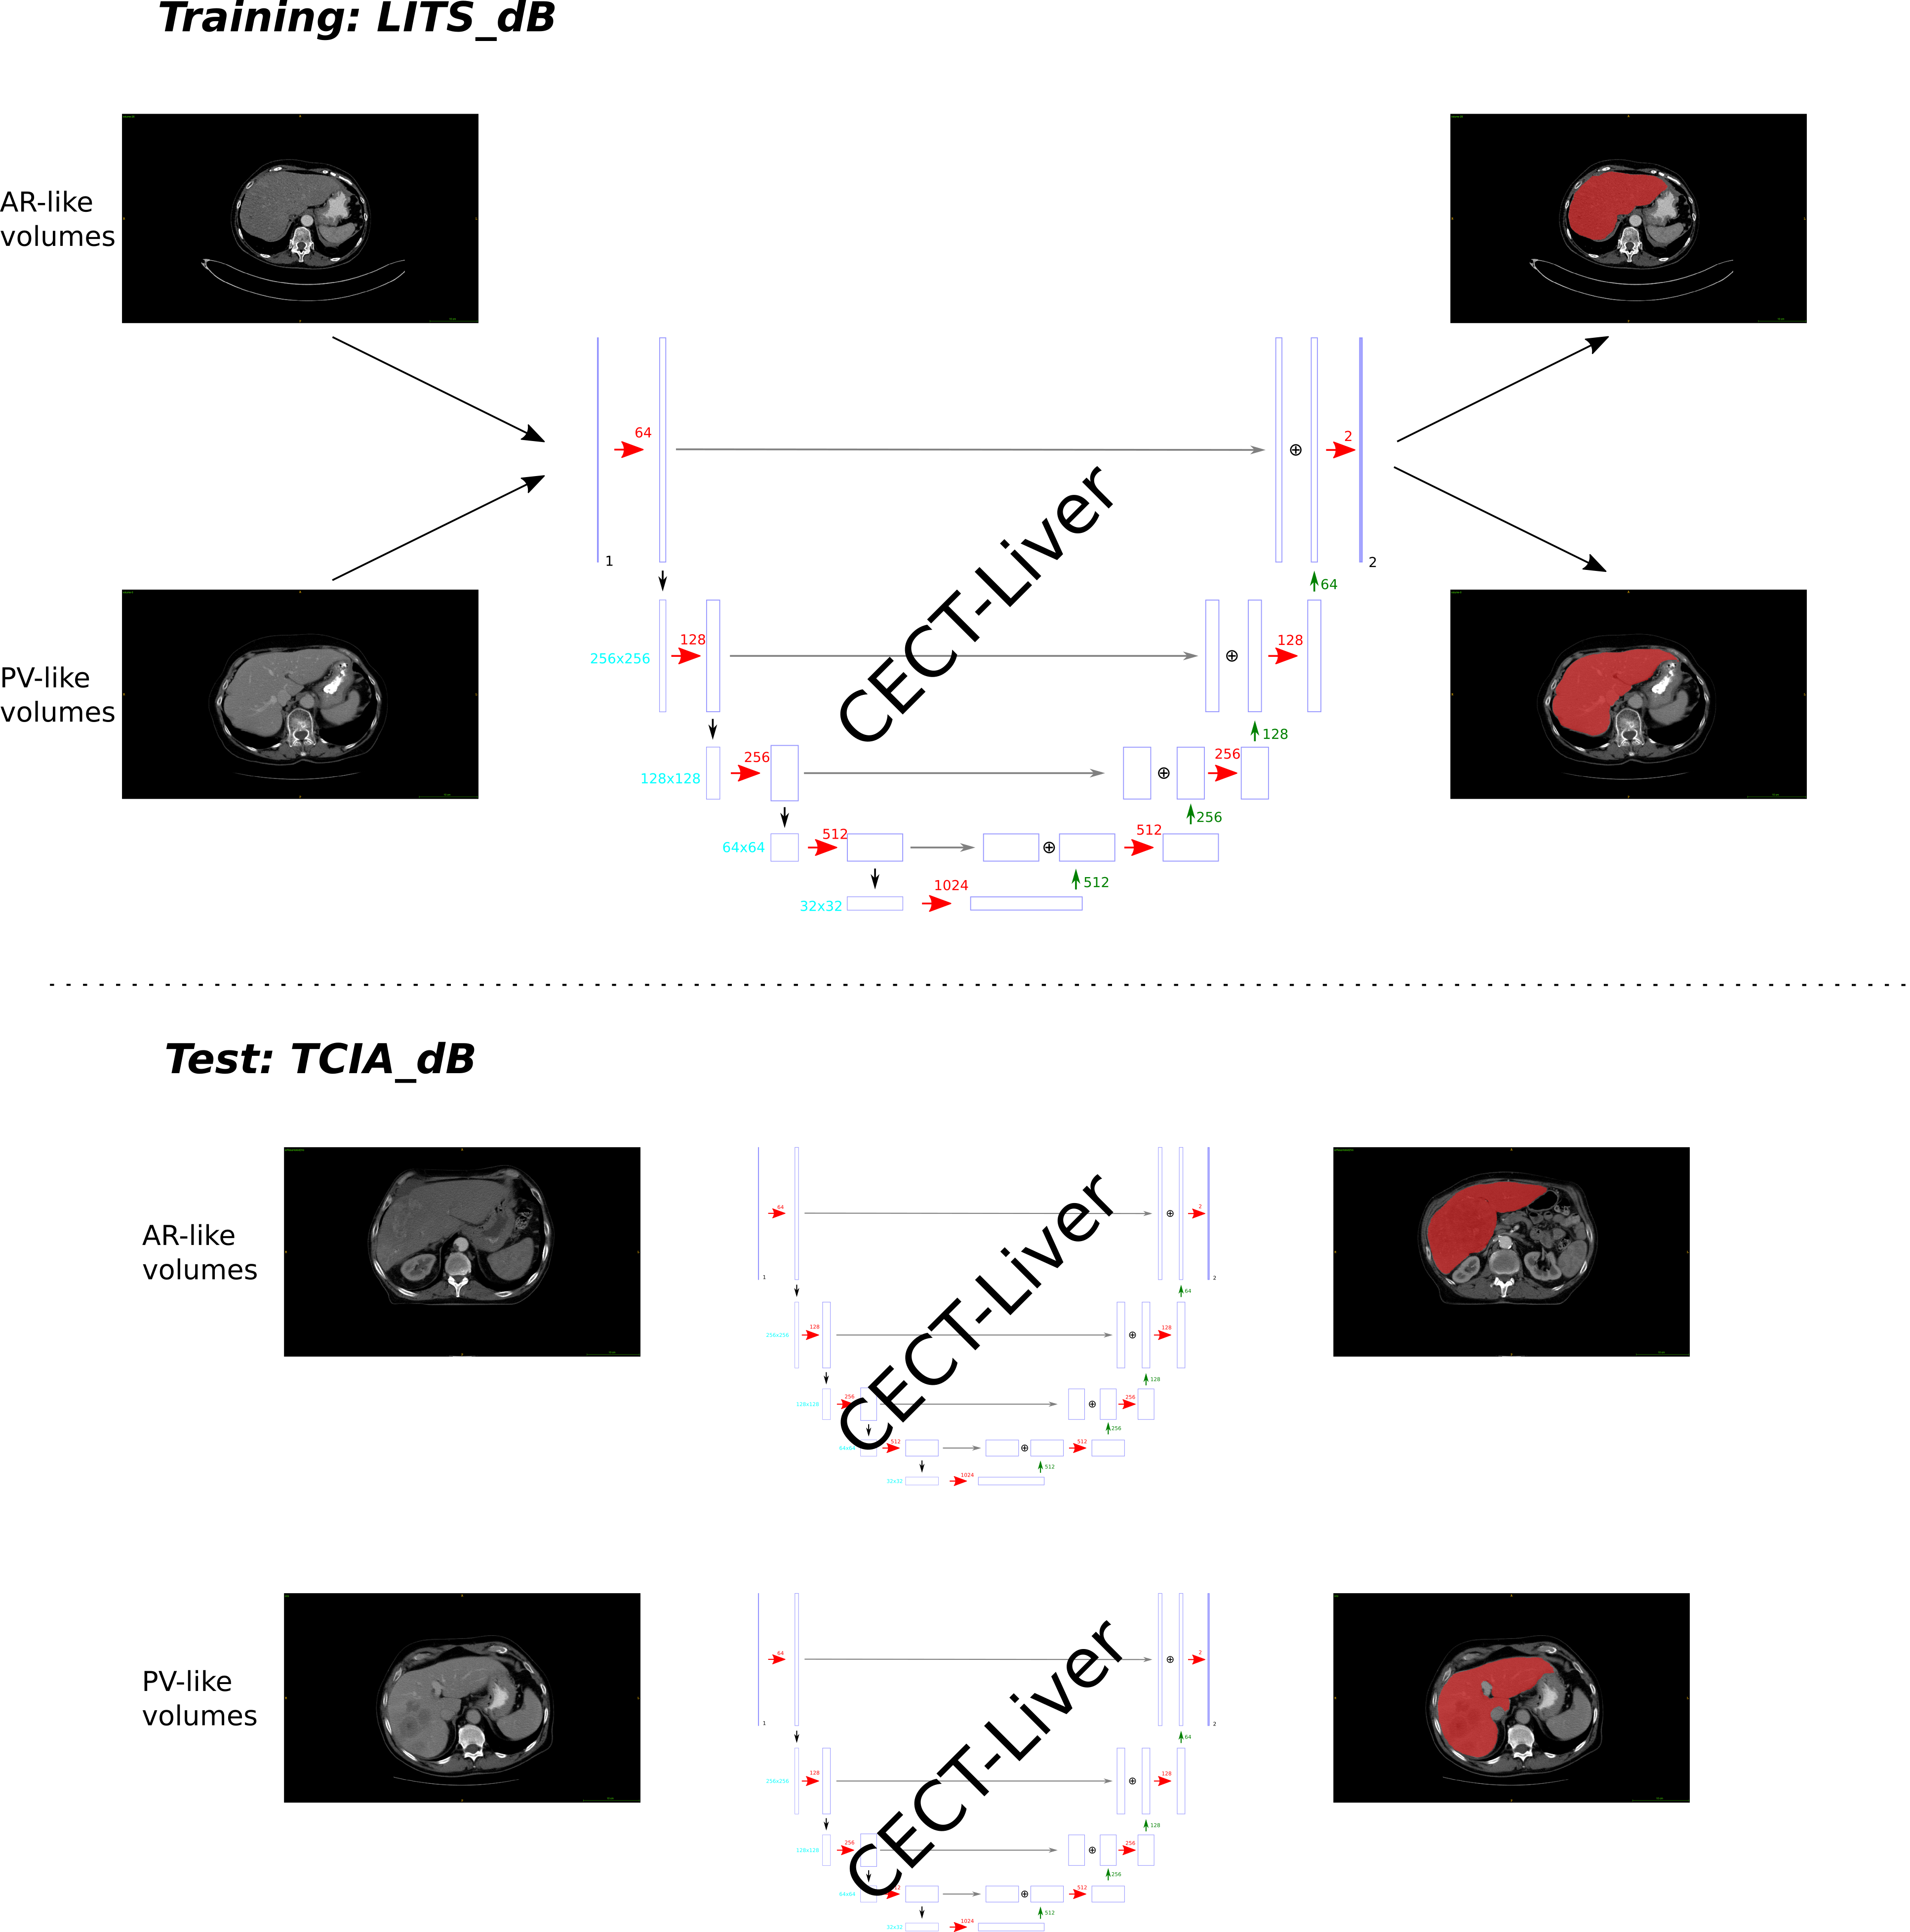
\includegraphics[width=\linewidth]{../Contributions/images/CECT_liver_details}
	\caption{We trained our network using each one of the 131 volumes of the \textbf{\lmttfont{LITS-dB}}, and tested the obtained architecture on both \ac{ar} and \ac{pv} \textbf{\lmttfont{TCIA-dB}} volumes. 
	}
	\label{fig:CECTliverDetails}
\end{figure}

Before training our multiphase tumor segmentation network, we have to ensure that both the liver and its internal structures such as the potential tumors are located at the same spatial position between
the different \ac{cect} volumes (both AR and PV volumes in our case). We therefore decided to register AR and PV volumes of the \textbf{\lmttfont{G-dB}} (training dataset) and the \textbf{\lmttfont{TCIA-dB}} (testing dataset) datasets.
We have decided to implement the registration pipeline using ANTs \cite{avants2009advanced}, since it has already been used for liver
CT scans registration \cite{Zhao2019,Zhao2020}.
During the registration process, the liver segmentation was used as
registration mask, and we decided to set the \ac{pv} volume as target (fixed)
volume since it usually presents the finer voxel resolution when
compared to \ac{ar} (or DELAY) volume. The registration pipeline described in the figure \ref{fig:RegistrationTCIA_pipeline_vertical2} was implemented as follows: we initially resampled the \ac{ar} volume so it has the same resolution as the corresponding \ac{pv} volume. We then performed the liver segmentation using \pplfont{\ac{cect}-Liver} on both the \ac{pv} and the resampled \ac{ar} volumes in a slice-wise manner with a classical post-processing consisting in applying a binary opening operation to the mask and conserving the big connected component (see green arrows in the figure \ref{fig:RegistrationTCIA_pipeline_vertical2}). We obtained a liver mask for both the \ac{pv} and the resampled \ac{ar} volumes. We finally applied the registration using a dilated version of the two masks obtained as registration masks (as depicted by the dashed blue arrows in the figure \ref{fig:RegistrationTCIA_pipeline_vertical2}; we dilated the liver mask with a SSE of 5cm when setting the registration mask in order to counter any error in the segmentation process, and to always have both the liver and its border included in the registration mask).

\begin{figure}[th!]
\centering
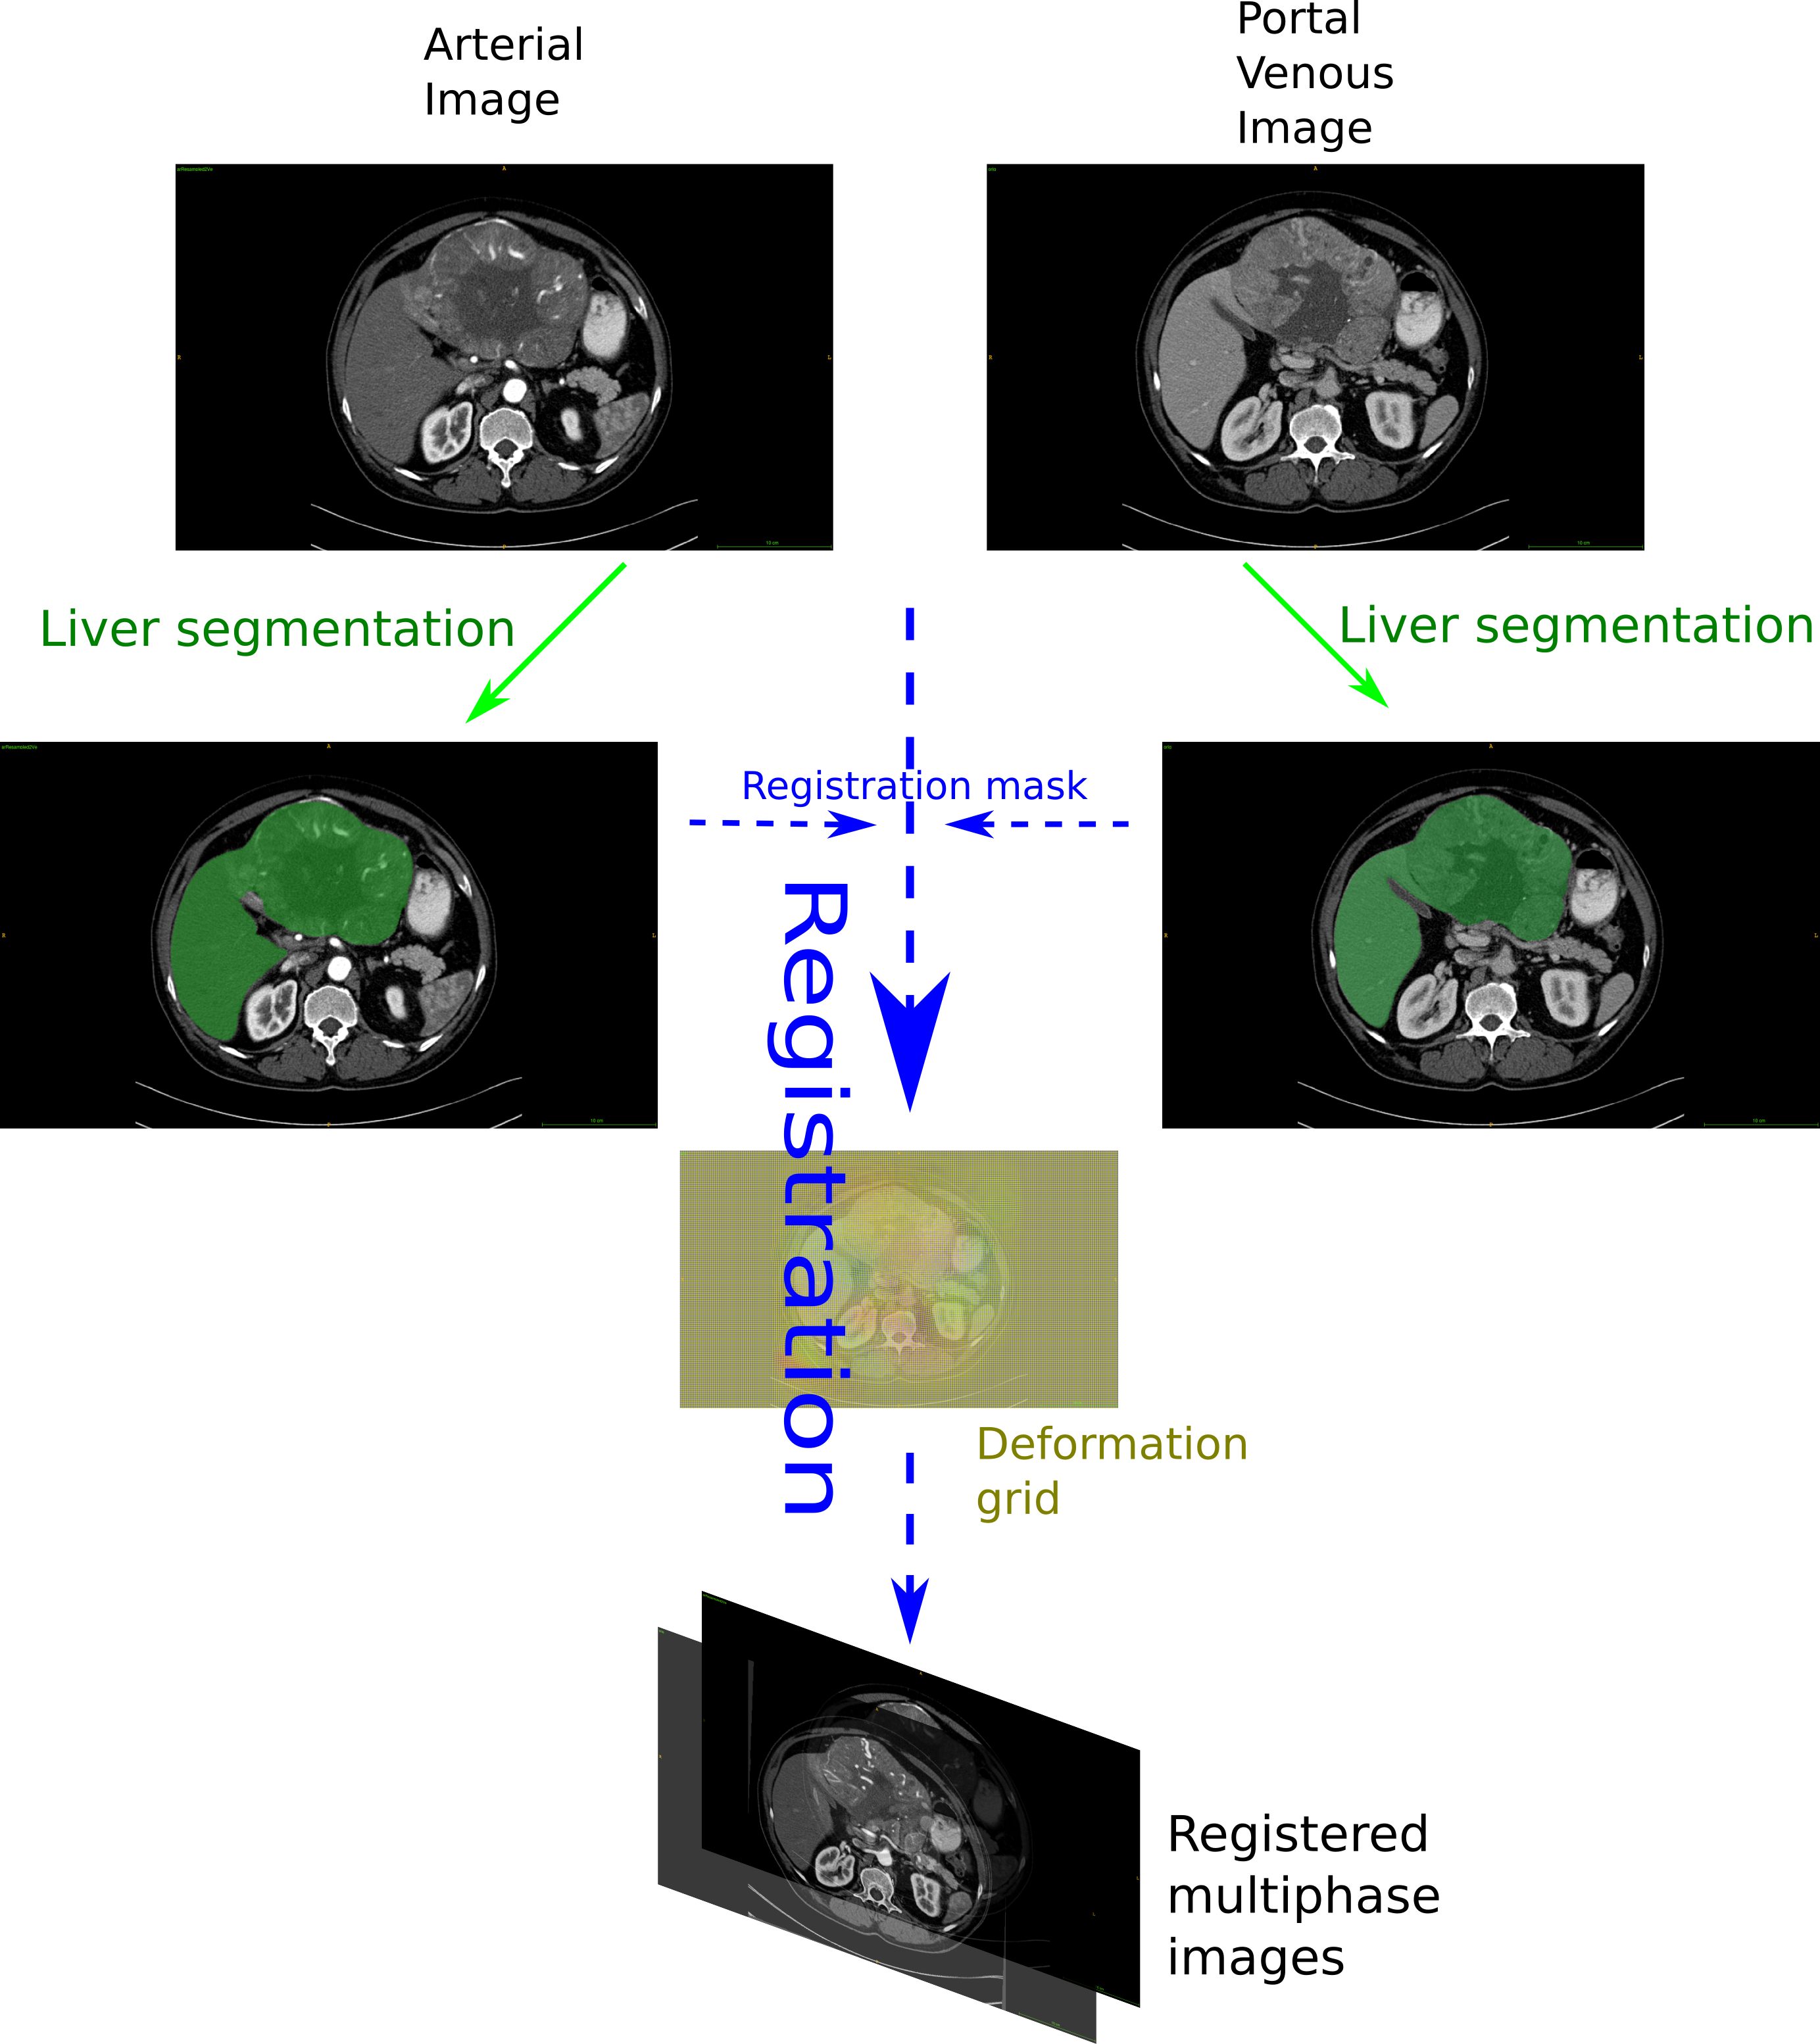
\includegraphics[width=0.7\linewidth]{../HistologicalGradePrediction/images/ResizeRegistrationTCIA_pipeline_vertical3}
\caption{Illustration of the registration pipeline applied to the images of \textbf{\lmttfont{TCIA-dB}}. The first green arrows correspond to the liver segmentation using a network trained on the \textbf{\lmttfont{LITS-dB}}. Dashed blue arrows correspond to the ANTs registration pipeline, where a dilated version of the predicted liver annotations maps are used as registration masks. The ANTs algorithm implements 3 transformations: a rigid, an affine, and a diffeomorphic Syn transformation that computes a deformation grid \cite{Avants2008}. The 3 steps of the ANTs algorithm allows us to obtain registered multiphase images.}
\label{fig:RegistrationTCIA_pipeline_vertical2}
\end{figure}

Once the volumes of both the training (\textbf{\lmttfont{G-dB}}) and the testing (\textbf{\lmttfont{TCIA-dB}}) datasets were registered, we trained our liver tumor segmentation network using the 79 volumes of the \textbf{\lmttfont{G-dB}} dataset by comparing both a \pplfont{MPF-Tumor} and a \pplfont{DMP-Tumor} (details regarding the architectures of the \pplfont{MPF-Tumor} and the \pplfont{DMP-Tumor} networks are given in the section \todo{add ref}).


\subsection{Histological grade prediction}\label{subsect_hist_grad_pred}

To perform the automatic histological grade prediction, we compare a traditional \ac{hcr}-based algorithm where features were extracted from either the automatically predicted or the expert-defined tumor ROI, and our \ac{dlr}-based algorithm where features were extracted from the second network of the cascaded tumor segmentation architecture before being processed by another neural network.\\
The \textbf{\lmttfont{TCIA-dB}} dataset with its associated annotations (liver and liver tumor segmentations) obtained thanks to the previous section (see section \ref{subsect_auto_liver_tumor_seg}) will be used to compared both the HCR and the DLR-based histological grade prediction pipelines.


\subsubsection{HCR-based histological grade prediction pipeline}\label{hcr-based_method}

We first performed the prediction of the histological grade using the \ac{hcr} features by extracting single-phase features (from either the AR or the PV volume).
In order to investigate the value brought by the dynamic information, we have decided either to perform the analysis on stacked single-phase features or to extract the features from a so-called \textit{perfusion} volume, where each voxel intensity corresponds to the difference between the \ac{pv} and the registered AR volume. An illustration of the process to obtain the \textit{perfusion} volume is given in the figure \ref{fig:perfusion}.

\begin{figure}
	\centering
	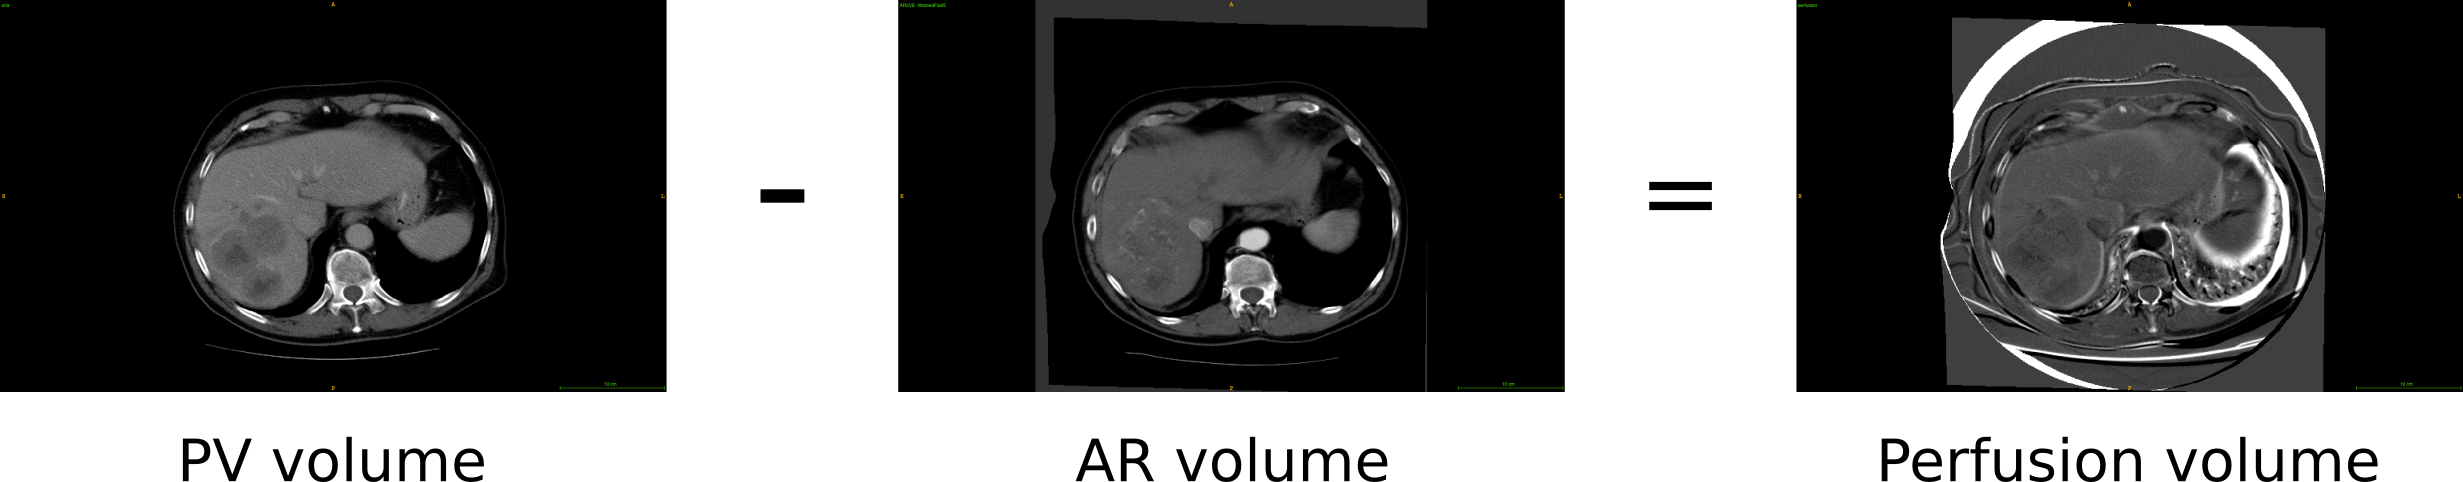
\includegraphics[width=0.9\linewidth]{../Contributions/images/perfusion}
	\caption{Left: Portal venous image, middle: registered AR image, right: perfusion image where each pixel's intensity is obtained by computing the difference between its PV and its AR intensity.}
	\label{fig:perfusion}
\end{figure}

The features extraction step was performed using the \textit{PyRadiomics} python module\footnote{\url{https://pyradiomics.readthedocs.io/en/latest/}}. This package allows the extraction of features on various representations of the raw image. In our case, we decided to extract features from both the original image and those obtained after application of LoG \footnote{Laplacian Of Gaussian with various $\sigma$ filter sizes} or Wavelet filtering methods. When using the original images, a total of 107 features are extracted, while only 93 features are extracted from the LoG filtered images (since shape-based features are removed). The wavelet filtering method produced 8 different images, hence a total of 744 features to extract (93 for each version). When combining all produced features for a single image, we reach a total of 944 features (when considering only one filter size for the LoG filtering step).
Once the features were extracted, a logistical model was built using the least absolute shrinkage and selection operator algorithm (LASSO). The objective is to minimize the negative log-likelihood contribution $L$ for each observation $ i $ of our training dataset, as described in the equation \ref{lassoLog}.
\begin{equation} \label{lassoLog}
L = -\sum_{i=1}^{N} \left[ y_{i} \left( {\beta}_{0} + {\beta}_{1} x_{i} \right) -\ln \left( 1+e^{({\beta}_{0} + {\beta}_{1} x_{i})} \right) \right] + \lambda \sum_{j=1}^{p} \left| {\beta}_{j} \right|
\end{equation}
Features are first normalized before the optimal $ \lambda  $ regularization parameter was selected. Features with non-zero coefficients $ \beta $ are retained for the construction of the predictive model.

The model was trained in a CV-manner and the histological grade was predicted patient-wise. The hyperparameters such as the $ \lambda $ regularization term were optimized at each fold and the accuracy of the model was computed by counting the number of correctly classified patients in the testing set throughout the entire cross-validation evaluation.

\subsubsection{DLR-based histological grade prediction architecture}\label{dlr-based_method}

The main drawbacks when implementing the \ac{hcr}-based pipeline were the method for the extraction of the dynamic features, the ROI to consider when extracting these features and finally the choice of features to extract from the images, that are often hand-crafted and may not encode the entire relevant information contained in the images.
To overcome these limitations, we created an automatic \ac{dlr}-based architecture for the prediction of the histological grade. The architecture was trained and tested on the 18 volumes of the \textbf{\lmttfont{TCIA-dB}} dataset.
The first step consisted on the automatic segmentation of the tumor on multiphase images, as described in the section \ref{subsect_auto_liver_tumor_seg}.
To predict the histological grade we decided to focus on what we called the
relevant imaging semantic features.

Before applying the extraction of the features, we normalized
the dimension of the different volumes of the dataset, so that each
voxel measures $ 0.68\times0.68 $mm in the axial plane (because it corresponds to
the resolution of the images used to train our semantic segmentation
network), and that the volumes have a 2.5mm z-spacing (corresponding to the
spacing of the majority of the \ac{pv} volumes in \textbf{\lmttfont{TCIA-dB}}).
When predicting the histological grade, we focused only on the centrally located tumor slices, since the histological grade corresponds to a measurement of the evolution of the
disease, which tends to have more physiological effects at the center of
the tumor. Centrally located slices will therefore exhibit the highest
grade for a given patient which in this case
corresponds to the observed patient-wise grade (ES1954 histological grading system \cite{EdmondsonHA1954}). It is worth noting that a slice-wise architecture was built, first because the features were computed in a slice-wise manner and second because the
histological grade tends to be heterogeneous in the lesion, meaning that
a slice-wise approach allows us to give a finer prediction to find
potential areas with a more advanced disease.

The network responsible for the multiphase segmentation of liver tumors is composed of 2 classical U-Net networks (as illustrated in the figure \todo{Add ref}), where each
one takes either the \ac{ar} or the \ac{pv} image as input. We believe
that the compressed information present in the bottleneck part of the
networks can be sufficient to encode the useful information present in the
image (the U-Net will work as an auto-encoder for the semantic information). Therefore, we extracted for each patient of the \textbf{\lmttfont{TCIA-dB}}, this
encoded information in a slice-wise manner, represented by two $ 32\times32\times512 $
features cubes (one per phase in the \pplfont{MPF-Tumor} architecture) per slice
as depicted in the figure \ref{fig:MPF_Features_Selection}.


\begin{figure}[!ht]
	\centering
	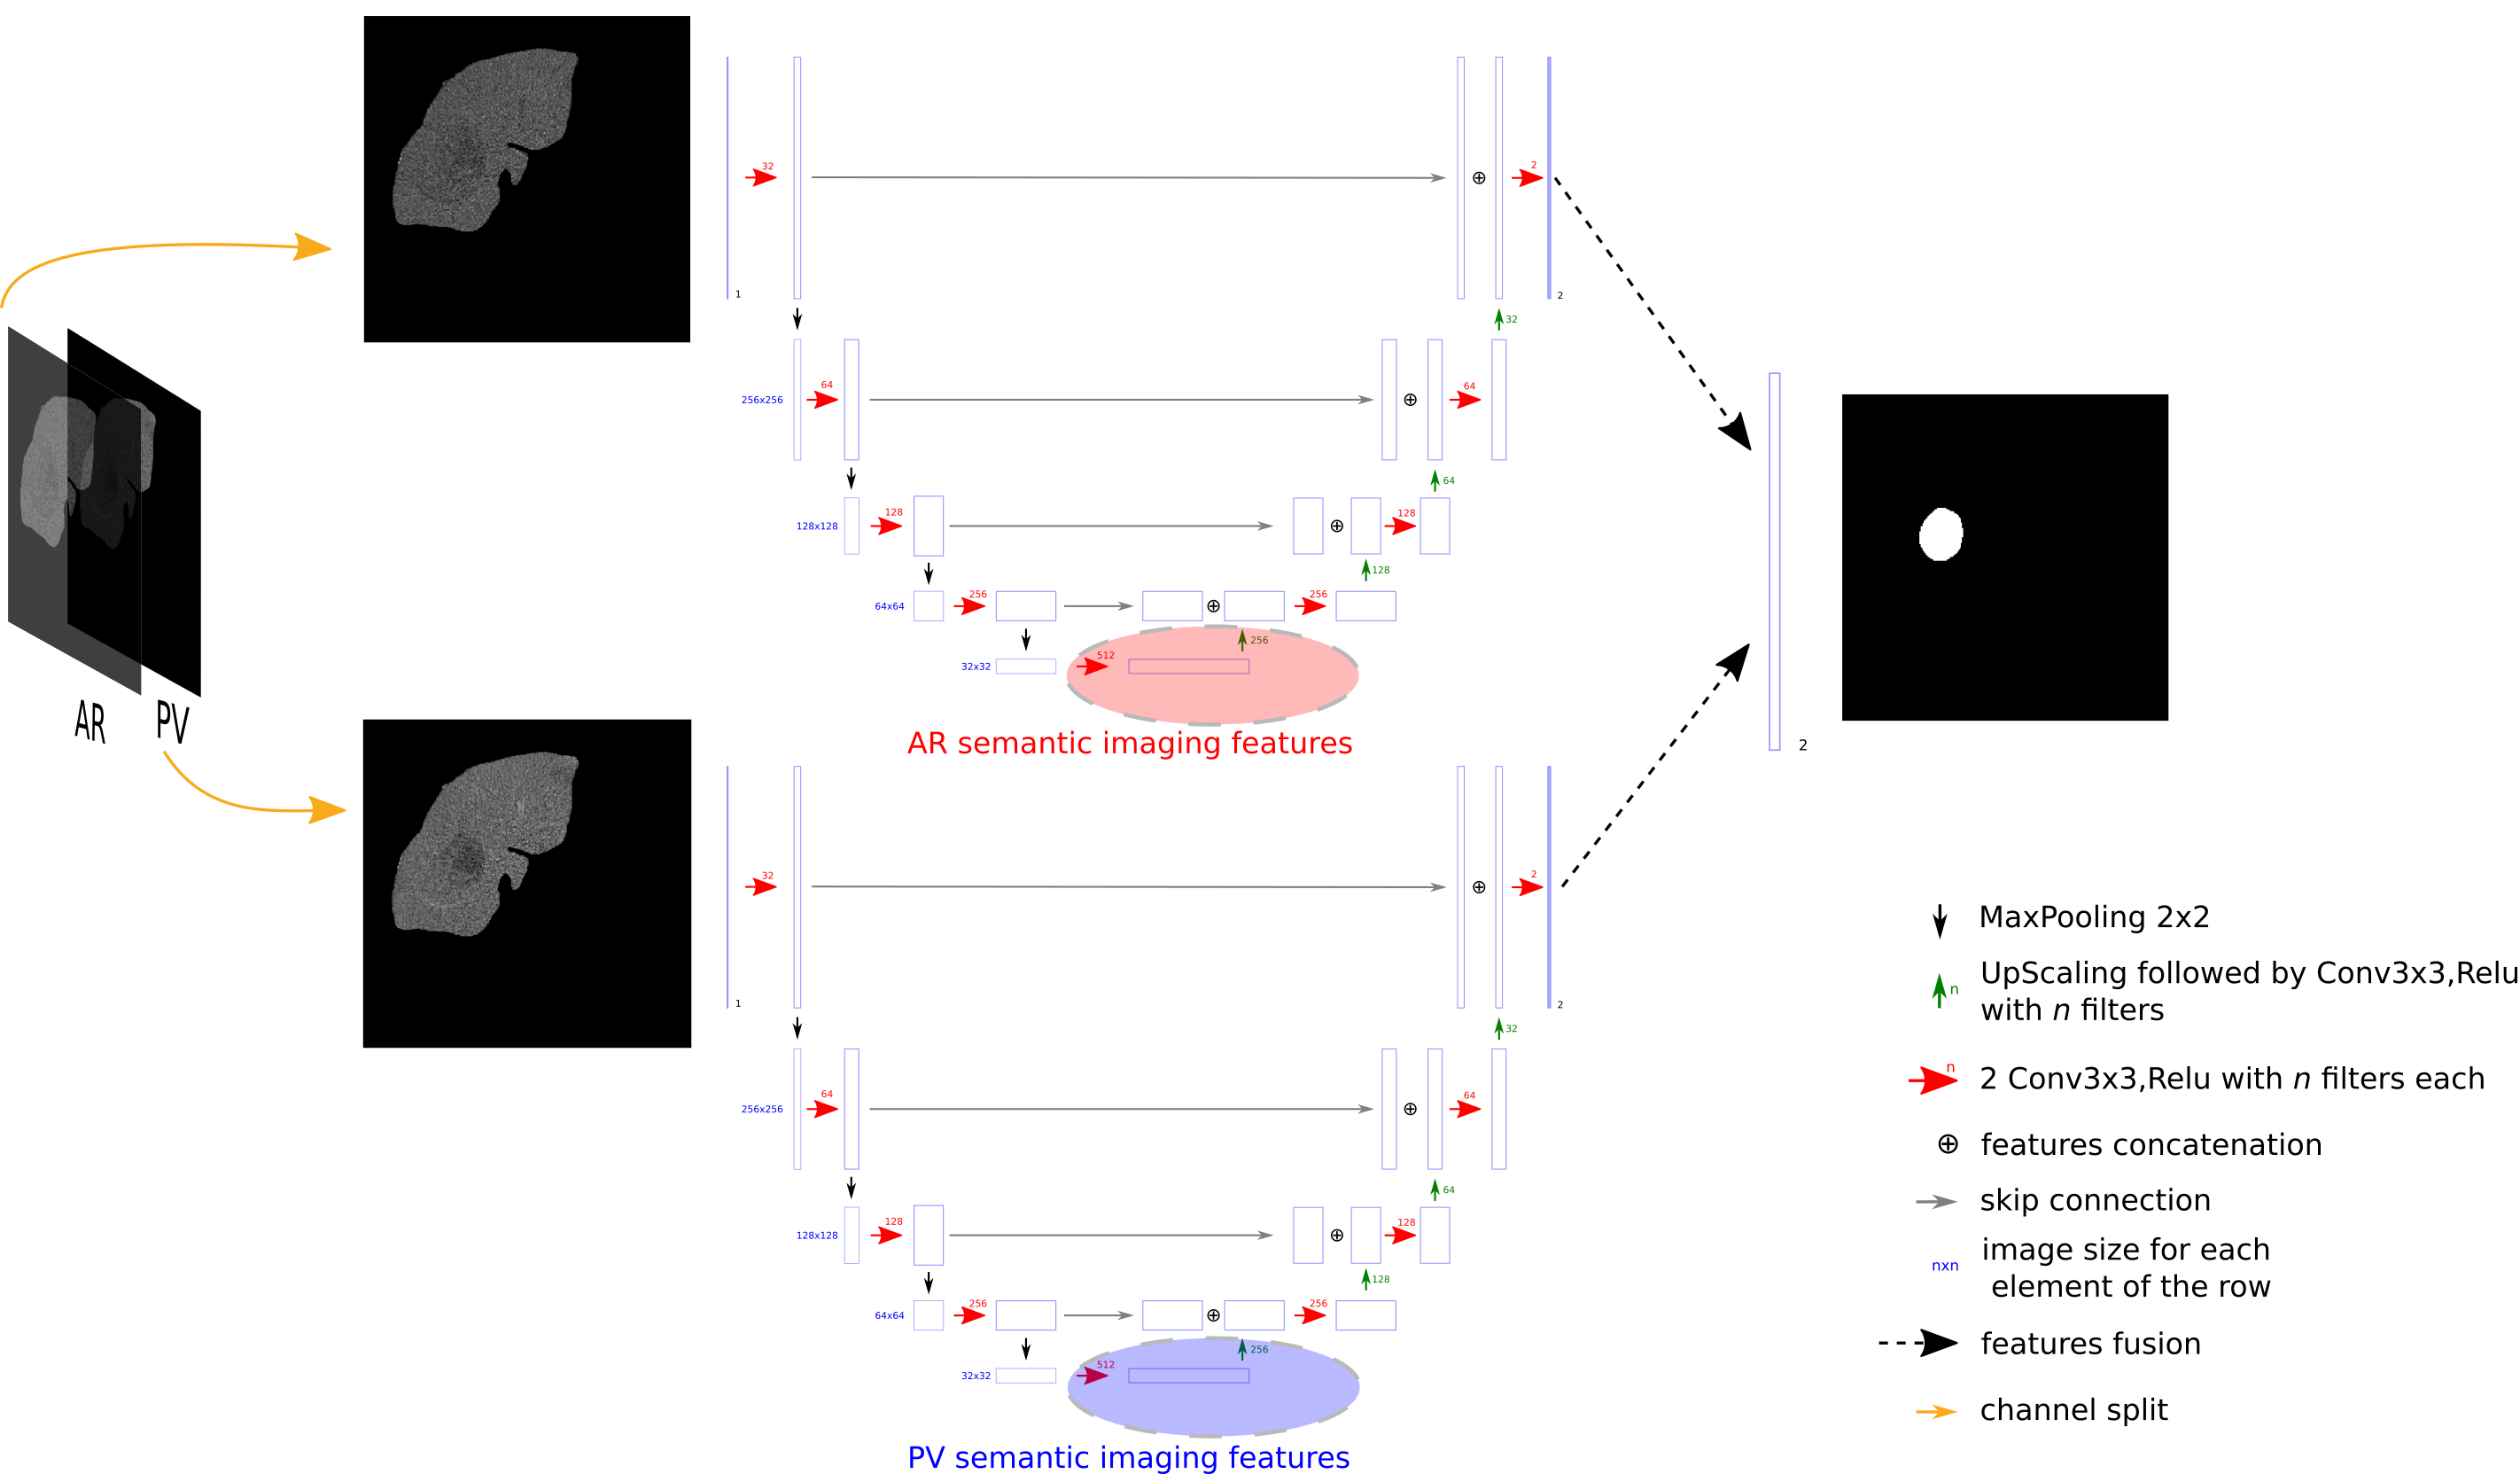
\includegraphics[width=0.95\linewidth]{../HistologicalGradePrediction/images/MPF_Features_Selection2}
	\caption{Red and blue areas correspond to the bottleneck part of the U-Net
	network where the features extraction is performed. Each image is then
	represented as a $ 32\times32\times512 $ features cube.}
	\label{fig:MPF_Features_Selection}
\end{figure}




\begin{figure}[!ht]
	\centering
	\includegraphics[width=0.9\linewidth]{../HistologicalGradePrediction/images/gradpredictionArchitecture}
	\caption{Slice-wise histological grade prediction using both \ac{ar} and \ac{pv} retained semantic imaging features}
	\label{fig:gradpredictionArchitecture}
\end{figure}

The architecture depicted in the figure \ref{fig:gradpredictionArchitecture} works as a dimensionality
reduction algorithm, where the first 1D convolutional layers are dedicated to
reduce the number of features initially present ($ 32\times32\times512 $). The
dimensionality reduction step is performed for each phase separately,
before the remaining features are combined (simple addition in the
features space).
A final dense layer takes the remaining features as input and computes
the probability of belonging to each class thanks to a softmax activation
function (LG vs HG).

Knowing the composition of \textbf{\lmttfont{TCIA-dB}} (9 high grade patients vs 9 low
grade ones), we performed a 9-fold CV training, so that each patient is
at least present once in the testing set, and so that the training and
the test sets contains both the same number of patients per
class (7 patients from each class in the training set and 1 patient from
each class in the testing set).

\section{Experiments \& Results}


\subsection{Liver tumor segmentation}
% Semantic segmentation results 

To obtain a quantitative evaluation of the prediction accuracy of our newly created
\pplfont{\ac{cect}-Liver} network, we tested it on the \textbf{\lmttfont{TheraHCC-dB}}. We
obtained a mean slice-wise \ac{dsc} of $ 90.4 \pm 17.5 $ on the \ac{pv} images and
$ 86.9 \pm 19.1 $ on the \ac{ar} images. These results, close to those obtained
in our previous work using a CV approach \cite{Ouhmich2019}, proved that \pplfont{\ac{cect}-Liver} can perform liver segmentation on both \ac{ar} and \ac{pv} unseen images.
The \pplfont{CECT-Liver} network was also able to segment unseen volumes of the
\textbf{\lmttfont{TCIA-dB}} in both \ac{ar} and \ac{pv} phases even when the liver presents a big lesion, as we can see in the figure \ref{fig:LiverPredTciaDb}.
Even though the overall visual predictions seemed very accurate, some mis-segmentation cases have been noticed. Liver segmentation errors often appear on top/bottom axial slices and are often due to our 2D approach, where the 3D context is lost, and where it is often very difficult to see the extremity of the liver in a single slice, as depicted in the figure \ref{fig:LITS_networkMisSeg_extremSlices}. As exposed previously, the main drawback of our approach corresponds to cases where the missed liver segment is occupied by a liver tumor (see \ref{fig:LITS_networkMisSeg_extremSlices} and \ref{fig:LITS_networkMisSeg_tumor}).
As explained earlier, an other problem often occurring is the mis-segmentation of other abdominal organs, that are sometimes considered as being part of the liver. However, our post-processing steps usually correct these mistakes by removing the undesired tissues from the final segmentation map (as illustrated in the figure \ref{fig:LITS_networkMisSeg_otherOrgans}).


\begin{figure}[ht!]
	\centering
	\begin{minipage}{0.45\linewidth}
		\includegraphics[width=0.9\linewidth]{../HistologicalGradePrediction/images/ResizeTCIA_CECTLiver_prediction_TCGA-DD-A11A_slice42_AR_raw}
	\end{minipage}
	\hspace{0.3cm}
	\begin{minipage}{0.45\linewidth}
		\includegraphics[width=0.9\linewidth]{../HistologicalGradePrediction/images/ResizeTCIA_CECTLiver_prediction_TCGA-DD-A11A_slice42_AR_green_liver}
	\end{minipage}
	\vspace{0.8cm}
	\begin{minipage}{0.45\linewidth}
		\includegraphics[width=0.9\linewidth]{../HistologicalGradePrediction/images/ResizeTCIA_CECTLiver_prediction_TCGA-DD-A11A_slice42_raw}
	\end{minipage}
	\hspace{0.3cm}
	\begin{minipage}{0.45\linewidth}
		\includegraphics[width=0.9\linewidth]{../HistologicalGradePrediction/images/ResizeTCIA_CECTLiver_prediction_TCGA-DD-A11A_slice42_greenLiver}
	\end{minipage}
	\caption{Example of liver segmentation using the \pplfont{\ac{cect}-Liver} network on \textbf{\lmttfont{TCIA-dB}}
	patients (Top row \ac{ar} images, bottom row: \ac{pv} images, left:
	Raw images, right : liver segmentation as overlay).}
	\label{fig:LiverPredTciaDb}
\end{figure}

\begin{figure}[ht!]
	\centering
	\begin{minipage}{0.45\linewidth}
		\includegraphics[width=\linewidth]{../Contributions/images/MisSegmentations/ResizeTCGA-DD-A3A1_slice80_raw}
	\end{minipage} \hspace{-0.1cm}
	\begin{minipage}{0.45\linewidth}
		\includegraphics[width=\linewidth]{../Contributions/images/MisSegmentations/ResizeTCGA-DD-A3A1_slice80_liverPrediction_Cmap}
	\end{minipage} \\
	\begin{minipage}{0.45\linewidth}
		\includegraphics[width=\linewidth]{../Contributions/images/MisSegmentations/ResizeTCGA-DD-A4NK_slice32_raw}
	\end{minipage} \hspace{-0.1cm}
	\begin{minipage}{0.45\linewidth}
		\includegraphics[width=\linewidth]{../Contributions/images/MisSegmentations/ResizeTCGA-DD-A4NK_slice32_liverPrediction_Cmap}
	\end{minipage} \\
	\begin{minipage}{0.45\linewidth}
		\includegraphics[width=\linewidth]{../Contributions/images/MisSegmentations/ResizeTCGA-DD-A1EB_slice9_raw}
	\end{minipage} \hspace{-0.1cm}
	\begin{minipage}{0.45\linewidth}
		\includegraphics[width=\linewidth]{../Contributions/images/MisSegmentations/ResizeTCGA-DD-A1EB_slice9_liverPrediction_Cmap_Arrow}
	\end{minipage}
	\caption{Examples of liver mis-segmentation cases with left being the raw images and right being the liver segmentation prediction obtained by our \pplfont{\ac{cect}-Liver} network (green area corresponds to the retained liver segmentation, whereas the purple area corresponds to voxels removed by the post-processing steps). Top row depicts an axial top liver slice, where nearly half of the liver has been missed. Second row depicts a bottom liver slice where a big portion of the liver occupied by a tumor has been missed by the liver segmentation. Bottom row also depicts a bottom liver slices where a small portion is missed by the network, but the hepatic lesion is missed as well (green arrow).}
	\label{fig:LITS_networkMisSeg_extremSlices}
\end{figure}

\begin{figure}[ht!]
	\centering
	\begin{minipage}{0.45\linewidth}
		\includegraphics[width=\linewidth]{../Contributions/images/MisSegmentations/ResizeTCGA-DD-A1EB_slice16_raw}
	\end{minipage} \hspace{-0.1cm}
	\begin{minipage}{0.45\linewidth}
		\includegraphics[width=\linewidth]{../Contributions/images/MisSegmentations/ResizeTCGA-DD-A1EB_slice16_liverPrediction_Cmap}
	\end{minipage}
	\caption{Example of liver mis-segmentation where a big portion of the lesion has been missed by our liver segmentation network. In this specific case, the portion of the tumor that has been missed corresponded to the necrotic area which was remarkably darker than usual (less than 10HU).}
	\label{fig:LITS_networkMisSeg_tumor}
\end{figure}

\begin{figure}[ht!]
	\centering
	\begin{minipage}{0.45\linewidth}
		\includegraphics[width=\linewidth]{../Contributions/images/MisSegmentations/ResizeTCGA-BC-A3KF_slice61_raw}
	\end{minipage} \hspace{-0.1cm}
	\begin{minipage}{0.45\linewidth}
		\includegraphics[width=\linewidth]{../Contributions/images/MisSegmentations/ResizeTCGA-BC-A3KF_slice61_liverPrediction_Cmap}
	\end{minipage} \\
	\begin{minipage}{0.45\linewidth}
		\includegraphics[width=\linewidth]{../Contributions/images/MisSegmentations/ResizeTCGA-BC-A10Z_slice30_raw}
	\end{minipage} \hspace{-0.1cm}
	\begin{minipage}{0.45\linewidth}
		\includegraphics[width=\linewidth]{../Contributions/images/MisSegmentations/ResizeTCGA-BC-A10Z_slice30_liverPrediction_Cmap}
	\end{minipage} \\
	\begin{minipage}{0.45\linewidth}
		\includegraphics[width=\linewidth]{../Contributions/images/MisSegmentations/ResizeTCGA-DD-A1EA_slice30_raw}
	\end{minipage} \hspace{-0.1cm}
	\begin{minipage}{0.45\linewidth}
		\includegraphics[width=\linewidth]{../Contributions/images/MisSegmentations/ResizeTCGA-DD-A1EA_slice30_liverPrediction_Cmap}
	\end{minipage}
	\caption{Examples of liver mis-segmentation cases with left being the raw images and right being the liver segmentation prediction obtained by our \pplfont{\ac{cect}-Liver} network (green area corresponds to the retained liver segmentation, whereas the purple area corresponds to voxels removed by the post-processing steps). In the given examples we have the stomach (top row), the spleen (second row) and the colon (bottom row) that have been mis-interpreted by the network as being part of the liver, however in each case the post-processing steps allowed us to remove the unwanted tissue from the remaining segmentation map.}
	\label{fig:LITS_networkMisSeg_otherOrgans}
\end{figure}

Regarding the liver tumor segmentation, we evaluated both \pplfont{DMP} and \pplfont{MPF}
architectures since no statistical differences were available when
comparing results obtained for the tumor segmentation in our previous
work on \textbf{\lmttfont{TheraHCC-dB}} \cite{Ouhmich2019}.

After training both architectures with the same parameters, we obtained a mean patient-wise \ac{dsc} of $ 73.2 \pm 20.6 $ with \pplfont{MPF}
architecture versus $ 64.9 \pm 27.2 $ when using the \pplfont{DMP} when evaluating the
models on the \textbf{\lmttfont{TCIA-dB}} patients. An example of prediction on the \textbf{\lmttfont{TCIA-dB}} is
depicted in figure \ref{fig:TCIAMultiphaseTumorPred}. 

\begin{figure}[ht!]
	\begin{minipage}{0.3\linewidth}
		\includegraphics[width=\linewidth]{../HistologicalGradePrediction/images/Resizeimage13.png}
	\end{minipage} \hspace{0.1cm}
	\begin{minipage}{0.3\linewidth}
		\includegraphics[width=\linewidth]{../HistologicalGradePrediction/images/Resizeimage10.png}
	\end{minipage} \hspace{0.1cm}
	\begin{minipage}{0.3\linewidth}
		\includegraphics[width=\linewidth]{../HistologicalGradePrediction/images/Resizeimage7.png}
	\end{minipage}
	\caption{Example of an image from the \textbf{\lmttfont{TCIA-dB}}, with the obtained predicted tumor segmentation using the \pplfont{MPF-Tumor} segmentation network (left: raw, middle: expert annotation, right: obtained segmentation)}
	\label{fig:TCIAMultiphaseTumorPred}
\end{figure}

These results obtained on an external dataset tend to demonstrate a satisfactory precision
of the tumor segmentation when training our cascaded architecture with a
sufficient number of cases.
For the second stage of the cascade, we retained the \pplfont{MPF-Tumor} segmentation network since it performed
significantly better than the \pplfont{DMP} one ($ p = 0.02 $ using a Wilcoxon signed
paired rank test on the patient-wise \ac{dsc}).
We confirmed the benefit of the cascaded architecture since these results
were obtained using an architecture where the first network was trained
on \textbf{\lmttfont{LITS-dB}} and the second on \textbf{\lmttfont{G-dB}}. Such an architecture allows consequently to obtain good results even though the number of training cases tends to be small, and the different available datasets homogeneous in the type of annotated areas. The cascaded architecture also permits to use a single-phase network for the first stage and a multiphasic network for the second.

\subsection{Histological grade prediction}

% histological grade prediction results HCR vs DLR
When evaluating the \ac{hcr}-based histological grade prediction model, we presented the accuracy of the model in terms of how many patients in the testing set were correctly classified throughout the 9-fold cross-validation training. Results are given in the table \ref{tab:hcrGrade}.
\renewcommand{\arraystretch}{2}
\begin{table}[!htp]
	\centering
	\caption{Accuracy of our HCR-based histological grade prediction model given the experimental settings. Results are given in terms of how many patients are correctly classified in the testing set during the CV process (over the 18 patients of the dataset).}\label{tab:hcrGrade}
	\scriptsize
	\begin{tabular}{lccccc}\toprule
		\multicolumn{2}{c}{Settings} &\multicolumn{4}{c}{Number of correctly classified patients (over 18)} \\\cmidrule{1-6}
		Image type &Tumor Segmentation & input = AR &input = PV &input = Perfusion & input = AR \& PV \\\midrule
		Original & Expert GT & 12  & 10  & 7 & 11 \\
		Original + LoG & Expert GT & 13  & 10  & 13 & 13 \\
		Original + LoG + Wavelet & Expert GT & 12  & 11  & 11 & 11 \\
		Original & predicted & 11  & 11  & 12 & 12 \\
		Original + LoG & predicted & \textbf{14}  & 12  & 13 & \textbf{14} \\
		Original + LoG + Wavelet & predicted & 9  & 10  & 10 & 11 \\
		\bottomrule
	\end{tabular}
\end{table}
\renewcommand{\arraystretch}{5}


The results highlighted that radiomics features extracted from the automatically predicted tumor ROI seemed to be as relevant as the ones extracted from the experts' defined tumor ROI. This indicates that our semantic segmentation network tends to retain relevant features (at least the features necessary for the wanted task).
The incorporation of LoG-based features seems to improve the predictive capacities of the model, and we also noticed that the accuracy was higher when filtering images with small filters (in our case 1mm filter gave the best results). This suggests that small details can be more important than larger ones for the determination of the histological grade, hence the necessity to create a model that aims for local prediction of histological grade to consider the heterogeneity within the tumor. We also realized that areas with low intensity within the tumor had their importance in the determination of the histological grade, especially the presence of necrotic areas, since most relevant features were glm-based features sensitive to small and large areas with low gray level intensity (SALGLE, SDLGLE and LRLGLE features) and intensity-based features sensitive to objects with low gray level intensity (first order $10^{th}$ percentile). 
When comparing the type of input, we realized that the best results were obtained when extracting features from the AR volumes, potentially meaning that the information relative to the histological grade is encoded through the difference between hypervascular structures of the tumor (more expressed in the AR-phase volumes) and the necrotic areas.


We finally compared the \ac{hcr}-based model with our \ac{dlr}-based newly created architecture.
After testing several combinations for the hyperparameters, we
fixed the number of retained features to 8 as depicted in the
figure \ref{fig:gradpredictionArchitecture} (meaning that after the features dimensionality reduction,
we obtained a $ 32\times32\times8 $ cube per phase), and we considered a 2cm volume
(corresponding to 8 centrally located slices with a 2.5mm spacing) when
training/testing our architecture.

With our CV-training, we were able to correctly predict the patient-wise
histological grade of \textbf{15 patients over the 18} of the dataset, as detailed in the table \ref{tab:confusion_matrix} (a patient is considered as being correctly predicted
when at least half of the retained slices were annotated with the
correct \ac{gt} class).
When considering a slice-wise prediction, we were able to correctly
predict \textbf{\textasciitilde{}74\%} of the slices.\\
It has been observed that the classification confidence was often correlated with the distance to the center of the tumor, where central tumor slices were correctly classified with a higher probability than distant slices, which were either classified with a lower confidence, or even misclassified, as we can see in the figure \ref{fig:Slice_hist_grad_prediction_2}. The quality of the semantic segmentation also often guided the accuracy of the prediction, as depicted in the figure \ref{fig:Slice_hist_grad_prediction_details}.

\begin{figure}[th!]
	\centering
	\includegraphics[width=0.9\linewidth]{../HistologicalGradePrediction/images/Slice_hist_grad_prediction_v3}
	\caption{Example of slice-wise histological grade prediction of one patient from the \lmttfont{TCIA-dB}. Here we observed that the confidence was correlated with the relative position to the center. Even though the semantic segmentation of the tumor was correctly performed, distant slices tend to be either misclassified or classified with a lower confidence than central slices. Details of tumor semantic segmentation are given for 3 slices (raw image where pixels outside the predicted liver are masked in the left side and where the tumor GT delineation is given in red, and tumor segmentation heatmap in the right side)}
	\label{fig:Slice_hist_grad_prediction_2}
\end{figure}


\begin{figure}[th!]
	\centering
	\includegraphics[width=0.9\linewidth]{../HistologicalGradePrediction/images/Slice_hist_grad_prediction_details_v2}
	\caption{Example of slice-wise histological grade prediction of one patient from the \lmttfont{TCIA-dB}. Here we observed that the confidence regarding the grade prediction was correlated with the quality of the semantic segmentation. An accurate semantic segmentation is therefore a prerequisite to extract relevant features. Details of tumor semantic segmentation are given for 3 slices (raw image where pixels outside the predicted liver are masked in the left side and where the tumor GT delineation is given in red, and tumor segmentation heatmap in the right side), two are correctly segmented and their histological grade was correctly predicted whereas one of them contained mis-segmented areas leading to a mis-classification of the histological grade.}
	\label{fig:Slice_hist_grad_prediction_details}
\end{figure}

\renewcommand{\arraystretch}{2}
\begin{table}[!ht]
	\centering
	\caption{Confusion matrix regarding the \ac{dlr}-based patient-wise histological grade prediction}\label{tab:confusion_matrix}
	\begin{tabular}{l|l|c|c|c}
		\multicolumn{2}{c}{}&\multicolumn{2}{c}{\textbf{True grade}}&\\
		\cline{3-4}
		\multicolumn{2}{c|}{}&LG&HG&\multicolumn{1}{c}{\textit{Total}}\\
		\cline{2-4}
		\multirow{2}{*}{\textbf{Predicted grade}}& LG & \textbf{7} & 1 & 8\\
		\cline{2-4}
		& HG & 2 & \textbf{8} & 10 \\
		\cline{2-4}
		\multicolumn{1}{c}{} & \multicolumn{1}{c}{\textit{Total}} & \multicolumn{1}{c}{\textbf{9}} & \multicolumn{1}{c}{9} & \multicolumn{1}{c}{18}\\
	\end{tabular}
\end{table}
\renewcommand{\arraystretch}{5}

These results provided a more detailed prediction than the one
consisting of a single patient-wise classification. Being able to
compute the histological grade locally (here in a slice-wise fashion)
allows us to visually focus on the heterogeneous regions that are
crucial when needing to establish a diagnosis. Our pipeline can also
provide a map of the best biopsy sites that will further be necessary in
the clinical practice to either evaluate the progression of the disease
or its prognosis.\\


\section{Conclusion}


We successfully confirmed that multiphase images incorporated in a cascaded architecture corresponds to the best combination when performing semantic segmentation of liver and its tumors. Moreover, our preliminary results proved that imaging features extracted from our cascaded multiphase segmentation architecture were relevant enough to be incorporated in a deep radiomics pipeline for the histological grade prediction. 
Compared to the \ac{hcr} features-based pipeline, our \ac{dlr} pipeline allows us to propose a way to predict the histological grade in a fully automatic fashion and at both a patient-wise and a slice-wise scale. 
It would have also been possible to compute the \ac{hcr} features in a slice-wise fashion but some of them would have lost their interpretability such as the shape-based features. The current DLR features-based pipeline allows us to perform the prediction in a fully automatic fashion with a better patient-wise accuracy as the one obtained with our HCR-based pipeline (15/18 patients correctly classified using the DLR-based pipeline vs 14/18 at best for the HCR-based pipeline).
Even though our results need to be validate by external studies, they tend to show that features extracted in an automatic fashion from the raw images can be more relevant than classical hand-crafted features.
Our histological grade prediction results were on par with the ones reported by the only study performing histological grade prediction but using a different dataset composed of MR images and using manually drawn regions of interest.\\
In the following section we present the different axes of improvement to improve the present work.


\newpage
%\bibliographystyle{unsrt}
\printbibliography[heading=bibintoc]

\end{document}